\documentclass[12pt]{tufte-book}
\usepackage{amsthm,amssymb,amsmath,thmtools,datetime,tikz}
\setcounter{secnumdepth}{3}

\declaretheorem[numberwithin=chapter,shaded={bgcolor=Lavender}]{definition}

\declaretheorem[numberwithin=chapter,shaded={bgcolor=Thistle}]{lemma}
\declaretheorem[numberwithin=chapter,shaded={bgcolor=Thistle}]{claim}

\declaretheorem[numberwithin=chapter,shaded={bgcolor=Apricot}]{theorem}

\declaretheorem[numberwithin=chapter,shaded={bgcolor=yellow}]{remark}
\declaretheorem[numberwithin=chapter]{exercise}
\declaretheorem[numberwithin=chapter,shaded={bgcolor=pink}]{construction}
\usepackage[
    type={CC},
    modifier={by-nc-nd},
    version={4.0},
]{doclicense}

\usepackage{graphicx,xcolor,mdframed}
%\usepackage[version=0.96]{pgf}
\usepackage{enumitem}


\def\chpcolor{blue!45}
\def\chpcolortxt{blue!60}

\iffalse
\titleformat{\chapter}%
  {\huge\rmfamily\itshape\color{red}}% format applied to label+text
  {\llap{\colorbox{red}{\parbox{1.5cm}{\hfill\itshape\huge\color{white}\thechapter}}}}% label
  {2pt}% horizontal separation between label and title body
  {}% before the title body
  []% after the title body
\fi

\hypersetup{colorlinks}% uncomment this line if you prefer colored hyperlinks (e.g., for onscreen viewing)

%%
% Book metadata
\title{A Course in Theory of Cryptography}
\author[Sanjam Garg]{Sanjam Garg}
%\publisher{Publisher of This Book}

%%
% If they're installed, use Bergamo and Chantilly from www.fontsite.com.
% They're clones of Bembo and Gill Sans, respectively.
%\IfFileExists{bergamo.sty}{\usepackage[osf]{bergamo}}{}% Bembo
%\IfFileExists{chantill.sty}{\usepackage{chantill}}{}% Gill Sans

%\usepackage{microtype}

%%
% Just some sample text
\usepackage{lipsum}
\newcommand{\ma}{\mathcal{A}}
\newcommand{\cA}{\mathcal{A}}
\newcommand{\mb}{\mathcal{B}}
\newcommand{\cB}{\mathcal{B}}

\newcommand{\getsr}{\xleftarrow{\$}}
\newcommand{\bit}{\{0,1\}}

\newcommand{\Gen}{\mathsf{Gen}}
\newcommand{\gen}{\mathsf{Gen}}
\newcommand{\Enc}{\mathsf{Enc}}
% \newcommand{\enc}{\mathsf{Enc}}
\newcommand{\Dec}{\mathsf{Dec}}
% \newcommand{\dec}{\mathsf{Dec}}
% \newcommand{\pk}{\mathsf{pk}}
% \newcommand{\sk}{\mathsf{sk}}
\newcommand{\ek}{\mathsf{ek}}

% \newcommand{\concat}[0]{\; || \;}

% \newcommand{\bin}{\{0,1\}}
% \newcommand{\adv}{\mathcal{A}}
% \newcommand{\advb}{\mathcal{B}}
% \newcommand{\advc}{\mathcal{C}}
% \newcommand{\fake}{\mathsf{FAKE}}

\newcommand{\Sign}{\mathsf{Sign}}
\newcommand{\Verify}{\mathsf{Verify}}
%\newcommand{\negl}{\mathsf{negl}}
\newcommand{\abort}{\mathsf{abort}}
\newcommand{\Sampler}{\mathsf{Sampler}}
\newcommand{\Eval}{\mathsf{Eval}}
\renewcommand{\tag}{\mathsf{tag}}
\newcommand{\PRF}{\mathsf{PRF}}
\newcommand{\LWE}{\mathsf{LWE}}
%%
% For nicely typeset tabular material
\usepackage{booktabs}

\usepackage[n,advantage,operators,sets,adversary,landau,probability,notions,logic,ff,mm,primitives,events,complexity,oracles,asymptotics,keys]{cryptocode} 
%%
% For graphics / images
\usepackage{graphicx,algpseudocode}
\setkeys{Gin}{width=\linewidth,totalheight=\textheight,keepaspectratio}
\graphicspath{{graphics/}}

% The fancyvrb package lets us customize the formatting of verbatim
% environments.  We use a slightly smaller font.
\usepackage{fancyvrb}
\fvset{fontsize=\normalsize}

%%
% Prints argument within hanging parentheses (i.e., parentheses that take
% up no horizontal space).  Useful in tabular environments.
\newcommand{\hangp}[1]{\makebox[0pt][r]{(}#1\makebox[0pt][l]{)}}

%%
% Prints an asterisk that takes up no horizontal space.
% Useful in tabular environments.
\newcommand{\hangstar}{\makebox[0pt][l]{*}}

%%
% Prints a trailing space in a smart way.
\usepackage{xspace}

%%
% Some shortcuts for Tufte's book titles.  The lowercase commands will
% produce the initials of the book title in italics.  The all-caps commands
% will print out the full title of the book in italics.
\newcommand{\vdqi}{\textit{VDQI}\xspace}
\newcommand{\ei}{\textit{EI}\xspace}
\newcommand{\ve}{\textit{VE}\xspace}
\newcommand{\be}{\textit{BE}\xspace}
\newcommand{\VDQI}{\textit{The Visual Display of Quantitative Information}\xspace}
\newcommand{\EI}{\textit{Envisioning Information}\xspace}
\newcommand{\VE}{\textit{Visual Explanations}\xspace}
\newcommand{\BE}{\textit{Beautiful Evidence}\xspace}

\newcommand{\TL}{Tufte-\LaTeX\xspace}

% Prints the month name (e.g., January) and the year (e.g., 2008)
\newcommand{\monthyear}{%
  \ifcase\month\or January\or February\or March\or April\or May\or June\or
  July\or August\or September\or October\or November\or
  December\fi\space\number\year
}


% Prints an epigraph and speaker in sans serif, all-caps type.
\newcommand{\openepigraph}[2]{%
  %\sffamily\fontsize{14}{16}\selectfont
  \begin{fullwidth}
  \sffamily\large
  \begin{doublespace}
  \noindent\allcaps{#1}\\% epigraph
  \noindent\allcaps{#2}% author
  \end{doublespace}
  \end{fullwidth}
}

% Inserts a blank page
\newcommand{\blankpage}{\newpage\hbox{}\thispagestyle{empty}\newpage}

\usepackage{units}

% Typesets the font size, leading, and measure in the form of 10/12x26 pc.
\newcommand{\measure}[3]{#1/#2$\times$\unit[#3]{pc}}

% Macros for typesetting the documentation
\newcommand{\hlred}[1]{\textcolor{Maroon}{#1}}% prints in red
\newcommand{\hangleft}[1]{\makebox[0pt][r]{#1}}
\newcommand{\hairsp}{\hspace{1pt}}% hair space
\newcommand{\hquad}{\hskip0.5em\relax}% half quad space
\newcommand{\TODO}{\textcolor{red}{\bf TODO!}\xspace}
\newcommand{\ie}{\textit{i.\hairsp{}e.}\xspace}
\newcommand{\eg}{\textit{e.\hairsp{}g.}\xspace}
\newcommand{\na}{\quad--}% used in tables for N/A cells
\providecommand{\XeLaTeX}{X\lower.5ex\hbox{\kern-0.15em\reflectbox{E}}\kern-0.1em\LaTeX}
\newcommand{\tXeLaTeX}{\XeLaTeX\index{XeLaTeX@\protect\XeLaTeX}}
% \index{\texttt{\textbackslash xyz}@\hangleft{\texttt{\textbackslash}}\texttt{xyz}}
\newcommand{\tuftebs}{\symbol{'134}}% a backslash in tt type in OT1/T1
\newcommand{\doccmdnoindex}[2][]{\texttt{\tuftebs#2}}% command name -- adds backslash automatically (and doesn't add cmd to the index)
\newcommand{\doccmddef}[2][]{%
  \hlred{\texttt{\tuftebs#2}}\label{cmd:#2}%
  \ifthenelse{\isempty{#1}}%
    {% add the command to the index
      \index{#2 command@\protect\hangleft{\texttt{\tuftebs}}\texttt{#2}}% command name
    }%
    {% add the command and package to the index
      \index{#2 command@\protect\hangleft{\texttt{\tuftebs}}\texttt{#2} (\texttt{#1} package)}% command name
      \index{#1 package@\texttt{#1} package}\index{packages!#1@\texttt{#1}}% package name
    }%
}% command name -- adds backslash automatically
\newcommand{\doccmd}[2][]{%
  \texttt{\tuftebs#2}%
  \ifthenelse{\isempty{#1}}%
    {% add the command to the index
      \index{#2 command@\protect\hangleft{\texttt{\tuftebs}}\texttt{#2}}% command name
    }%
    {% add the command and package to the index
      \index{#2 command@\protect\hangleft{\texttt{\tuftebs}}\texttt{#2} (\texttt{#1} package)}% command name
      \index{#1 package@\texttt{#1} package}\index{packages!#1@\texttt{#1}}% package name
    }%
}% command name -- adds backslash automatically
\newcommand{\docopt}[1]{\ensuremath{\langle}\textrm{\textit{#1}}\ensuremath{\rangle}}% optional command argument
\newcommand{\docarg}[1]{\textrm{\textit{#1}}}% (required) command argument
\newenvironment{docspec}{\begin{quotation}\ttfamily\parskip0pt\parindent0pt\ignorespaces}{\end{quotation}}% command specification environment
\newcommand{\docenv}[1]{\texttt{#1}\index{#1 environment@\texttt{#1} environment}\index{environments!#1@\texttt{#1}}}% environment name
\newcommand{\docenvdef}[1]{\hlred{\texttt{#1}}\label{env:#1}\index{#1 environment@\texttt{#1} environment}\index{environments!#1@\texttt{#1}}}% environment name
\newcommand{\docpkg}[1]{\texttt{#1}\index{#1 package@\texttt{#1} package}\index{packages!#1@\texttt{#1}}}% package name
\newcommand{\doccls}[1]{\texttt{#1}}% document class name
\newcommand{\docclsopt}[1]{\texttt{#1}\index{#1 class option@\texttt{#1} class option}\index{class options!#1@\texttt{#1}}}% document class option name
\newcommand{\docclsoptdef}[1]{\hlred{\texttt{#1}}\label{clsopt:#1}\index{#1 class option@\texttt{#1} class option}\index{class options!#1@\texttt{#1}}}% document class option name defined
\newcommand{\docmsg}[2]{\bigskip\begin{fullwidth}\noindent\ttfamily#1\end{fullwidth}\medskip\par\noindent#2}
\newcommand{\docfilehook}[2]{\texttt{#1}\index{file hooks!#2}\index{#1@\texttt{#1}}}
\newcommand{\doccounter}[1]{\texttt{#1}\index{#1 counter@\texttt{#1} counter}}

% Generates the index
\usepackage{makeidx}
\makeindex

\begin{document}
\iffalse
% Front matter
\frontmatter

% r.1 blank page
\blankpage


% v.2 epigraphs
\newpage\thispagestyle{empty}
\openepigraph{%
The public is more familiar with bad design than good design.
It is, in effect, conditioned to prefer bad design, 
because that is what it lives with. 
The new becomes threatening, the old reassuring.
}{Paul Rand%, {\itshape Design, Form, and Chaos}
}
\vfill
\openepigraph{%
A designer knows that he has achieved perfection 
not when there is nothing left to add, 
but when there is nothing left to take away.
}{Antoine de Saint-Exup\'{e}ry}
\vfill
\openepigraph{%
\ldots the designer of a new system must not only be the implementor and the first 
large-scale user; the designer should also write the first user manual\ldots 
If I had not participated fully in all these activities, 
literally hundreds of improvements would never have been made, 
because I would never have thought of them or perceived 
why they were important.
}{Donald E. Knuth}
\fi

% r.3 full title page
\maketitle


% v.4 copyright page
%\newpage
\begin{fullwidth}
~\vfill
\thispagestyle{empty}
\setlength{\parindent}{0pt}
\setlength{\parskip}{\baselineskip}
Copyright \copyright\ \the\year\ \thanklessauthor

%\par\smallcaps{Published by \thanklesspublisher}

\par\smallcaps{This document is continually being updated. Please send us your feedback.}


\par \doclicenseThis
 \index{license}

\par\textit{This draft was compiled on \today.}
\end{fullwidth}

% r.5 contents
\tableofcontents

%\listoffigures

%\listoftables

% r.7 dedication
\iffalse
\cleardoublepage
~\vfill

\begin{doublespace}
\noindent\fontsize{18}{22}\selectfont\itshape
\nohyphenation
Dedicated to those who appreciate \LaTeX{} 
and the work of \mbox{Edward R.~Tufte} 
and \mbox{Donald E.~Knuth}.
\end{doublespace}
\vfill
\vfill

% r.9 introduction
\cleardoublepage
\fi
\chapter*{Preface}
Cryptography enables many paradoxical objects, such as public key encryption, verifiable electronic signatures, zero-knowledge protocols, and fully homomorphic encryption.  The two main steps in developing such seemingly impossible primitives are (i) defining the desired security properties formally and (ii) obtaining a construction satisfying the security property provably. In modern cryptography, the second step typically assumes (unproven) computational assumptions, which are conjectured to be computationally intractable. In this course, we will define several cryptographic primitives and argue their security based on well-studied computational hardness assumptions. However, we will largely ignore the mathematics underlying the assumed computational intractability assumptions.

\section*{Acknowledgements}
These lecture notes are based on scribe notes taken by students in CS 276 over the years. Also, thanks to Peihan Miao, Akshayaram Srinivasan, and Bhaskar Roberts for helping to improve these notes.
%%
% Start the main matter (normal chapters)
\newcommand{\sanjam}[1]{{\color{red} Sanjam: #1}}

\newcommand{\bhaskar}[1]{{\color{ForestGreen} Bhaskar: #1}}

\mainmatter
\chapter{Mathematical Background}
\label{sec:mb}

In modern cryptography, (1) we typically assume that our attackers cannot run in unreasonably large amounts of time, and (2) we allow security to be broken with a \emph{very small}, but non-zero, probability.

Without these assumptions, we must work in the realm of information-theoretic cryptography, which is often unachievable or impractical for many applications. For example, the one-time pad --- an information-theoretically secure cipher --- is not very useful because it requires very large keys.

In this chapter, we define items (1) and (2) more formally. We require our adversaries to run in polynomial time, which captures the idea that their runtime is not unreasonably large (sections~\ref{ssec:ppt}). We also allow security to be broken with negligible -- very small -- probability (section ~\ref{ssec:nnf}). 


\section{Probabilistic Polynomial Time}
\label{ssec:ppt}
A probabilistic Turing Machine is a generic computer that is allowed to make random choices during its execution. A probabilistic \textit{polynomial time} Turing Machine is one which halts in time polynomial in its input length. More formally:

\begin{definition}[Probabilistic Polynomial Time]
A probabilistic Turing Machine $M$ is said to be PPT (a Probabilistic Polynomial Time Turing Machine) if $\exists c \in \mathbb{Z}^+$ such that $\forall x \in\{0,1\}^*$, $M(x)$ halts in $|x|^c$ steps.
\end{definition}

A {\em non-uniform} PPT Turing Machine is a collection of machines one for each input length, as opposed to a single machine that must work for all input lengths.

\begin{definition}[Non-uniform PPT]
A non-uniform PPT machine is a sequence of Turing Machines $\{ M_1, M_2, \cdots \}$ such that $\exists c \in \mathbb{Z}^+$ such that $\forall x \in\{0,1\}^*$, $M_{|x|}(x)$ halts in $|x|^c$ steps.
\end{definition}



\section{Noticeable and Negligible Functions}
\label{ssec:nnf}
Noticeable and negligible functions are used to characterize the ``largeness'' or ``smallness'' of a function describing the probability of some event.  Intuitively, a noticeable function is required to be larger than some inverse-polynomially function in the input parameter. On the other hand, a negligible function must be smaller than any inverse-polynomial function of the input parameter. More formally:


\begin{definition}[Noticeable Function]
A function $\mu(\cdot): \mathbb{Z}^+ \rightarrow [0,1]$ is noticeable iff $\exists c \in \mathbb{Z}^+, n_0 \in \mathbb{Z}^+$ such that $\forall n \geq n_0 , \; \mu(n) \geq n^{-c}$.
\end{definition}

\paragraph{Example.} Observe that $\mu(n) = n^{-3}$ is a noticeable function.  (Notice that the above definition is satisfied for $c = 3$ and $n_0 = 1$.)

\begin{definition}[Negligible Function]
A function $\mu(\cdot): \mathbb{Z}^+ \rightarrow [0,1]$ is negligible iff $\forall c \in \mathbb{Z}^+ \; \exists n_0 \in \mathbb{Z}^+$ such that $\forall n \geq n_0 , \; \mu(n) < n^{-c}$.
\end{definition}

\paragraph{Example.} $\mu(n) = 2^{-n}$ is an example of a negligible function. This can be observed as follows.
Consider an arbitrary $c \in \mathbb{Z}^+$ and set $n_0 = c^2$. Now, observe that for all $n \geq n_0$, we have that $\frac{n}{\log_2 n} \geq \frac{n_0}{\log_2 n_0} \geq \frac{n_0}{\sqrt{n_0}} = \sqrt{n_0} = c$. This allows us to conclude that $$\mu(n) = 2^{-n} = n^{-\frac{n}{\log_2 n}} \leq n^{-c}.$$

Thus, we have proved that for any $c \in \mathbb{Z}^+$, there exists $n_0 \in \mathbb{Z}^+$ such that for any $n \geq n_0$, $\mu(n) \leq n^{-c}$.

\paragraph{Gap between Noticeable and Negligible Functions.}
At first thought it might seem that a function that is {not} negligible (or, a non-negligible function) must be a noticeable. This is not true!\cite{JC:Bellare02} Negating the definition of a negligible function, we obtain that a non-negligible function $\mu(\cdot)$ is such that $\exists c \in \mathbb{Z}^+$ such that $\forall n_0 \in \mathbb{Z}^+$, $\exists n \geq n_0$ such that $\mu(n) \geq n^{-c}$.
Note that this requirement is satisfied as long as $\mu(n) \geq n^{-c}$ for infinitely many choices of $n \in \mathbb{Z}^+$. However, a noticeable function requires this condition to be true for every $n \geq n_0$.

Below we give example of a function $\mu(\cdot)$ that is neither negligible nor noticeable.
$$\mu(n) = \Big\{
\begin{array}{ll}
  2^{-n} & : x \mod 2 = 0\\
  n^{-3} & : x \mod 2 \neq 0
\end{array}
$$
This function is obtained by interleaving negligible and  noticeable functions. It cannot be negligible (resp., noticeable) because it is greater (resp., less) than an inverse-polynomially function for infinitely many input choices.

\paragraph{Properties of Negligible Functions.} Sum and product of two negligible functions is still a negligible function. We argue this for the sum function below and defer the problem for products to Exercise~\ref{ex:product}.

\begin{exercise}
If $\mu(n)$ and $\nu(n)$ are negligible functions from domain $\mathbb{Z}^+$ to range $[0,1]$ then prove that the following functions are also negligible:
\begin{enumerate}
    \item $\psi_1(n) = \frac{1}{2} \cdot \left(\mu(n) + \nu(n)\right)$
    \item $\psi_2(n) = \mu(n)\cdot \nu(n)$
    \item $\psi_3(n) = \mathsf{poly}(\mu(n))$, where $\mathsf{poly}(\cdot)$ is an unspecified polynomial function.
\end{enumerate}function.
\end{exercise}
\proof 
$ $
\begin{enumerate}
    \item We need to show that for any $c \in \mathbb{Z}^+$, we can find $n_0$ such that $\forall n \geq n_0$, $\psi_1(n) \leq n^{-c}$. Our argument proceeds as follows. Given the fact that $\mu$ and $\nu$ are negligible we can conclude that there exist $n_1$ and $n_2$ such that $\forall n \geq n_1$, $\mu(n) \leq n^{-c}$ and $\forall n \geq n_2$, $g(n) \leq n^{-c}$. Combining the above two facts and setting $n_0 = \max(n_1, n_2)$ we have that for every $n \geq n_0$,
    \begin{align*}
        \psi_1(n) &= \frac{1}{2} \cdot (\mu(n) + \nu(n)) \leq \frac{1}{2} \cdot (n^{-c} + n^{-c}) = n^{-c}
    \end{align*}
    Thus, $\psi_1(n) \leq n^{-c}$ and hence is negligible.
\end{enumerate}
\qed

%\begin{corollary}
%If $f(n)$ is non-negligible and $g(n)$ is negligible, then $h(n) = f(n) - g(n)$ is non-negligible.
%\end{corollary}
%
%\proof If $h(n)$ was negligible, then $f(n) = g(n) + h(n)$ would be the sum of two negligible functions, but would be non-negligible, which is a contradiction.  \qed


\newcommand{\binset}[1]{\{0,1\}^{#1}}
\newcommand{\binfunc}[2]{\binset{#1}\rightarrow\binset{#2}}
\newcommand{\bin}{\{0,1\}}
\newcommand{\adv}{\mathcal{A}}
\newcommand{\advb}{\mathcal{B}}
\newcommand{\advc}{\mathcal{C}}

\chapter{One-Way Functions}
\label{sec:owf}

\label{ssec:owf}
Cryptographers often attempt to base cryptographic results on conjectured computational assumptions to leverage reduced adversarial capabilities. Furthermore, the security of these constructions is no better than the assumptions they are based on. 
\begin{quote}
\emph{Cryptographers seldom sleep well.}\footnote{Quote by Silvio Micali in personal communication with Joe Kilian.}
\end{quote}
Thus, basing cryptographic tasks on the \emph{minimal} necessary assumptions is a key tenet in cryptography. Towards this goal, rather can making assumptions about specific computational problem in number theory, cryptographers often consider \emph{abstract primitives}. The existence of these abstract primitives can then be based on one or more computational problems in number theory.

The weakest abstract primitive cryptographers consider is one-way functions. Virtually, every cryptographic goal of interest is known to imply the existence of one-way functions. In other words, most cryptographic tasks would be impossible if the existence of one-way functions was ruled out. On the flip side, the realizing cryptographic tasks from just one-way functions would be ideal. 

\section{Definition}
A one-way function $f: \{0,1\}^n \rightarrow \{0,1\}^m$ is a function that is easy to compute but hard to invert. This intuitive notion is trickier to formalize than it might appear on first thought.

\begin{definition}[One-Way Functions]
A function $f : \binset{*} \rightarrow \binset{*}$ is said to be one-way function if:
\begin{itemize}
\item[-] \textbf{Easy to Compute:} $\exists$ a (deterministic) polynomial time machine $M$ such that $\forall x \in \binset{*}$ we have that \[M(x) = f(x)\]

\item[-] \textbf{Hard to Invert:} $\forall$ non-uniform PPT adversary $\mathcal{A}$ we have that
    \begin{equation}\label{eq:owf}
    \mu_{\mathcal{A},f}(n) = \Pr_{x \stackrel{\$}{\leftarrow} \binset{n}}[ \mathcal{A}(1^n, f(x)) \in f^{-1}(f(x))]
     \end{equation}
     is a negligible function,  $x \overset{\$}{\leftarrow} \binset{n}$ denotes that $x$ is drawn uniformly at random from the set $\binset{n}$, $f^{-1}(f(x)) = \{x' \mid f(x) = f(x')\}$, and the probability is over the random choices of $x$ and the random coins of $\mathcal{A}$\footnotemark.
\end{itemize}
\end{definition}

\begin{marginfigure}[-10cm]
\begin{tikzpicture}
    % ellipse
    \draw[black,fill=yellow!50] (0,0) ellipse (1cm and 2cm)
    node at (0,0) {$\{0,1\}^n$};
    \draw[black,fill=orange!50] (3,0) ellipse (1cm and 2cm) 
    node at (3,0) {$\{0,1\}^m$};
    % lines connecting ellipses
    \draw[green!40!black!100, thick, ->] (0.5,0.75) -- (2.5,0.75) node[midway, above] {Easy to Compute};
    \draw[red!40!black!100, thick, dashed, ->] (2.5,-0.75) -- (0.5,-0.75) node[midway, below] {Hard to Invert};
\end{tikzpicture}
\caption{Visulizing One-way Funcations}
\label{fig:owf}
\end{marginfigure}


\footnotetext{Typically, the probability is only taken over the random choices of $x$, since we can fix the random coins of the adversary $\mathcal{A}$ that maximize its advantage.}

We note that the function is not necessarily one-to-one. In other words, it is possible that $f(x) = f(x')$ for $x \neq x'$ -- and the adversary is allowed to output any such $x'$.

The above definition is rather delicate. We next describe problems in the slight variants of this definition that are insecure.

\begin{enumerate}
\item What if we require that
    $\Pr_{x \stackrel{\$}{\leftarrow} \binset{n}}[ \mathcal{A}(1^n, f(x)) \in f^{-1}(f(x))] = 0$ instead of being negligible?

This condition is false for every function $f$. An adversary $\mathcal{A}$ that outputs an arbitrarily fixed value $x_0$ succeeds with probability at least $1/2^{n}$, as $x_0 = x$ with at least the same probability.

\item  What if we drop the input $1^n$ to $\mathcal{A}$ in Equation~\ref{eq:owf}?

Consider the function $f(x) = |x|$.  In this case, we have that $m = \log_2 n$, or $n = 2^m$.  Intuitively, $f$ should not be considered a one-way function, because it is easy to invert $f$. Namely, given a value $y$ any $x$ such that $|x| = y$ is such that $x \in f^{-1}(y)$.  However, according to this definition the adversary gets an $m$ bit string as input, and hence is restricted to running in time polynomial in $m$. Since each possible $x$ is of size $n = 2^m$, the adversary doesn't even have enough time to write down the answer!  Thus, according to the flawed definition above, $f$ would be a one-way function.

Providing the attacker with $1^n$ ($n$ repetitions of the $1$ bit) as additional input avoids this issue.  In particular, it allows the attacker to run in time polynomial in $m$ and $n$.
\end{enumerate}

\paragraph{Candidate One-way Functions.}
It is not known whether one-way functions exist. In fact, the existence of one-way functions would imply that $P \neq NP$ (see Exercise~\ref{ex:PNP}). 

However, there are candidates of functions that could be one-way functions, based on the difficulty of certain computational problems. One example is based on the hardness of factoring. Multiplication can be done easily in $O(n^2)$ time, but so far no polynomial time algorithm is known for factoring.
Explicitly, we can define the function $f_1 : P_n \times P_n \rightarrow \mathbb{Z}$ where $P_n$ is the set of all $n$-bit primes as $f_1(p, q) = p \cdot q$.

% One candidate might be to say that given an input $x$, split $x$ into its left and right halves $x_1$ and $x_2$, and then output $x_1 \times x_2$.  However, this is not a one-way function, because with probability $\frac{3}{4}$, $2$ will be a factor of $x_1 \times x_2$, and in general the factors are small often enough that a non-negligible number of the outputs could be factored in polynomial time.

% To improve this, we again split $x$ into $x_1$ and $x_2$, and use $x_1$ and $x_2$ as seeds in order to generate large primes $p$ and $q$, and then output $pq$.  Since $p$ and $q$ are primes, it is hard to factor $pq$, and so it is hard to retrieve $x_1$ and $x_2$.  This function is believed to be one-way.

Another candidate is based on the hardness of the discrete logarithm problem. Given a group $\mathbb{G}$ of prime order $q$ and a generator $g$, the discrete logarithm problem is to find $x$ such that $g^x = y$ for a given $y$. The function $f_2 : \mathbb{Z}_q \rightarrow \mathbb{G}$ defined as $f_2(x) = g^x$ is also believed to be one-way assuming the hardness of the discrete logarithm problem.


\section{Robustness and Brittleness of One-way Functions}
What operations can we perform on one-way functions and still have a one-way function? In this section, we explore the robustness and brittleness of one-way functions and some operations that are safe or unsafe to perform on them.

\subsection{Robustness}
Consider having a one-way function $f$.  Can we use this function $f$ in order to make a more structured one-way function $g$ such that $g(x_0) = y_0$ for some constants $x_0, y_0$, or would this make the function no longer be one-way? 

Intuitively, the answer is yes - we can specifically set $g(x_0) = y_0$, and otherwise have $g(x) = f(x)$.  In this case, the adversary gains the knowledge of how to invert $y_0$, but that will only happen with negligible probability, and so the function is still one-way.

% \begin{theorem}
% Given a one-way function $f : \binset{n} \rightarrow \binset{m}$ and constants $x_0 \in \binset{n}$, $y_0 \in \binset{m}$, $\exists g : \binset{n} \rightarrow \binset{m}$ such that $g(x_0) = y_0$ where $g$ is a one-way function.
% \end{theorem}

In fact, this can be done for an exponential number of $x_0, y_0$ pairs. To illustrate that, consider the following function:
\[
  g(x_1\|x_2) = \left\{ \begin{array}{ll} x_1\|x_2 & : x_1 = 0^{n/2} \\ f(x_1\|x_2) & : \text{otherwise} \end{array} \right.
\]

However, this raises an apparent contradiction - according to this theorem, given a one-way function $f$, we could keep fixing each of its values to $0$, and it would continue to be a one-way function.  If we kept doing this, we would eventually end up with a function which outputs 0 for {\em all} of the possible values of $x$.  How could this still be one-way?\\

The resolution of this apparent paradox is by noticing that a one-way function is only required to be one-way in the limit where $n$ grows very large.  So, no matter how many times we fix the values of $f$ to be 0, we are still only setting a finite number of $x$ values to 0.  However, this will still satisfy the definition of a one-way function - it is just that we will have to use larger and larger values of $n_0$ in order to prove that the probability of breaking the one-way function is negligible.

\subsection{Brittleness}
\paragraph{Example: OWFs do not always compose securely.}
Given a one-way function $f : \binfunc{n}{n}$, is the function $f^2(x) = f(f(x))$ also a one-way function?  Intuitively, it seems that if it is hard to invert $f(x)$, then it would be just as hard to invert $f(f(x))$. 
% \sanjam{Explain the intuitive reduction that doesn't work.}  
However, this intuition is incorrect and highlights the delicacy when working with cryptographic assumptions and primitives. In particular, assuming one-way functions exists we describe a one-way function $f: \{0,1\}^{n}\times \{0,1\}^{n} \rightarrow \{0,1\}^{2n}$ such that $f^2$ can be efficiently inverted.
Let $g: \{0,1\}^n \rightarrow \{0,1\}^n$ be a one-way function then we set $f$ as follows:
$$f(x_1,x_2) = 0^{n}\|g(x_1)$$
Two observations follow:
\begin{enumerate} 
  \item $f^2$ is not one-way. This follows from the fact that for all inputs $x_1, x_2$ we have that $f^2(x_1,x_2) = 0^{2n}$. This function is clearly not one-way!
  \item $f$ is one-way. This can be argued as follows. Assume that there exists an adversary $\mathcal{A}$ such that $\mu_{\mathcal{A},f}(n) = \Pr_{x \stackrel{\$}{\leftarrow} \binset{n}}[ \mathcal{A}(1^{2n}, f(x)) \in f^{-1}(f(x))]$ is non-negligible. Using such an $\mathcal{A}$ we will describe a construction of adversary $\mathcal{B}$ such that $\allowbreak\mu_{\mathcal{B},g}(n) = \Pr_{x \stackrel{\$}{\leftarrow} \binset{n}}[ \mathcal{B}(1^n, g(x)) \in g^{-1}(g(x))]$ is also non-negligible. This would be a contradiction thus proving our claim.

      \textbf{Description of $\mathcal{B}$}: $\mathcal{B}$ on input $y \in\{0,1\}^n$ outputs the $n$ lower-order bits of  $\mathcal{A}(1^{2n}, 0^{n}\|y)$.

      Observe that if $\mathcal{A}$ successfully inverts $f$ then we have that $\mathcal{B}$ successfully inverts $g$. More formally, we have that:
      $$\mu_{\mathcal{B},g}(n) = \Pr_{x \stackrel{\$}{\leftarrow} \binset{n}}\left[ \mathcal{A}(1^{2n}, 0^n || g(x)) \in \{0,1\}^n || g^{-1}(g(x))\right].$$
      But
      \begin{align*}
      \mu_{\mathcal{A},f}(2n) =& \Pr_{x_1, x_2 \stackrel{\$}{\leftarrow} \binset{2n}}[ \mathcal{A}(1^{2n}, f(x_1, x_2)) \in f^{-1}(f(\tilde x))]\\
      = & \Pr_{x_1 \stackrel{\$}{\leftarrow} \binset{n}}[ \mathcal{A}(1^{2n}, 0^n || g(x_2)) \in \{0,1\}^n || g^{-1}(g(x_2))] \\
      = & \mu_{\mathcal{B},g}(n).
      \end{align*}
      Hence, we have that $\mu_{\mathcal{B},g}(n) = \mu_{\mathcal{A},f}(2n)$ which is non-negligible as long as $\mu_{\mathcal{A},f}(2n)$  is non-negligible.
\end{enumerate}


%\begin{lemma}
%If $f : \binfunc{n}{n}$ is a one-way function, then $g : \binfunc{2n}{2n}$ defined as $g(x) = 0^n \concat f(x_{[1:n]})$ is also one-way.\\
%\end{lemma}
%\proof
%Assume towards contradiction that $g$ is not one-way, and so there is an adversary $A_g$ that inverts $g$ with probability $\mu(2n)$ that is non-negligible.\\
%
%Note that $\mu(2n)$ is also non-negligible with respect to inputs of size $n$.\\

%Then we can define an adversary $A_f$ such that $A_f(y) = (A_g(0^n \concat y))_{[1:n]}$.  Note that $A_g$ breaks $g$ on input $0^n \concat y$ $\implies$ $A_f$ breaks $f$ on input $y$, and so $A_f$ breaks $f$ with at least non-negligible probability $\mu(2n)$.  Contradiction.\\
%
%Thus, $g$ is also one-way.  \qed\\
%
%Now, given a function $f : \binfunc{n}{n}$, we can construct a new one-way function $g : \binfunc{2n}{2n}$.  From $g$, we can construct another one-way function $h : \binfunc{2n}{2n}$ defined by:
%
%$h(x) = \left\{
%\begin{array}{lr}
%  0^{2n} & : x_{[1:n]} = 0^n \\
%  g(x) & : otherwise
%\end{array}
%\right.$

%A generalization of the previous theorem (fixing values in a one-way function) shows that $h$ is also a one-way function.  (In short, we are only fixing the values of $\frac{2^n}{2^{2n}} = \frac{1}{2^n}$ of all of the possible values of $x$.  Since we are only fixing a negligible fraction of the possible values of $x$, the same proof with slight modifications still applies.)\\
%
%So, $h$ is a one-way function.  However, $h^2(x) = h(h(x)) = 0^{2n}$, and so $h^2$ is clearly not a one-way function.  Thus, composing one-way functions is not guaranteed to give another one-way function. \qed

%\usepackage[utf8]{inputenc}
%\usepackage{amsmath,amssymb,fullpage}


% The goal of this section is to illustrate the general strategy for the problems of the form,
% \begin{center}
% \textit{``If $f$ is one-way function, then show that $f'$ (derived from $f$) is not a one-way function"}
% \end{center}
% Some of the examples include:
% \begin{itemize}
% \item If $f$ is a one-way function, prove that $f'$ defined as $f(f(\cdot))$ is not one-way.
% \item If $f$ is a one-way function, prove that $f'$ defined by dropping the first bit the output of $f$ is not one-way.
% \end{itemize}

% In order to give such a proof, we need to give an example of an one-way function $f$ and show that $f'$ (derived from $f$) is not one-way. The general strategy for these types of problems is the following:
% \begin{enumerate}
% \item Come up with a contrived function $g$ and show that $g$ is one-way. 
% \item Construct the new function $g'$ that is derived from $g$.
% \item Show that $g'$ can be inverted with non-negligible probability and thus show that $g'$ is not one-way.
% \end{enumerate}
% The reason why we need to come-up with a contrived function is that for specific one-way function $f$, $f'$ (derived from $f$) could be one-way. To see why this is the case, consider a one-way function $f: \bin^n \rightarrow \bin^n$ that is additionally injective. Then, one can show that $f^2(\cdot)$ is in fact a one-way function.\footnote{Try to prove this!} On the other hand, in the previous section, we showed that there exists a (contrived) function $g$ such that $g$ is one-way but $g^2$ is not one-way.
% Hence, we might not always be able to start from any one-way function $f$ and show that $f'$ (derived from $f$) is not one-way. The first step where we come up a suitable $g$ requires some ingenuity. Once that is done, the second and the third steps would generally be not so hard.

% To illustrate these three steps, let us consider a concrete example. 

\paragraph{Example: Dropping a bit is not always secure.}
Below is another example of a transformation that does not work. Given any one-way function $g$, let $g'(x)$ be $g(x)$ with the first bit omitted.

\begin{claim}
$g'$ is not necessarily one-way. In other words, there exists a OWF function $g$ for which $g'$ is not one-way.
\end{claim}
\begin{proof}
We must (1) construct a function $g$, (2) show that $g$ is one-way, and (3) show that $g'$ is not one-way.


\noindent\textbf{Step 1: Construct a OWF $g$.} 
To do this, we first want to come up with a (contrived) function $g$ and prove that it is one-way.
Let us assume that there exists a one-way function $h : \bin^n \rightarrow \bin^n$. We define the function $g : \bin^{2n} \rightarrow \bin^{2n}$ as follows:
$$
g(x\|y) = \begin{cases}
 0^{n}\|y &\text{    if } x = 0^n\\
1\|0^{n-1}\|g(y) &\text{    otherwise }
\end{cases}
$$

\noindent\textbf{Step 2: Prove that $g$ is one-way.}

\begin{claim}
If $h$ is a one-way function, then so is $g$.
\end{claim}
\begin{proof}
Assume for the sake of contradiction that $g$ is not one-way. Then there exists a polynomial time adversary $\adv$ and a non-negligible function $\mu(\cdot)$ such that:
$$
\Pr_{x,y}[\adv(1^n,g(x\|y)) \in g^{-1}(g(x\|y))] = \mu(n)
$$
We will use such an adversary $\adv$ to invert $h$ with some non-negligible probability. This contradicts the one-wayness of $h$ and thus our assumption that $g$ is not one-way function is false.

Let us now construct an $\advb$ that uses $\adv$ and inverts $h$. $\advb$ is given $1^n,h(y)$ for a randomly chosen $y$ and its goal is to output $y' \in h^{-1}(h(y))$ with some non-negligible probability. $\advb$ works as follows:
\begin{enumerate}
\item It samples $x \gets \bin^n$ randomly.
\item If $x = 0^n$, it samples a random $y' \gets \bin^n$ and outputs it.
\item Otherwise, it runs $\adv(10^{n-1}\|h(y))$ and obtains $x' \| y'$. It outputs $y'$.
\end{enumerate}

Let us first analyze the running time of $\advb$. The first two steps are clearly polynomial (in $n$) time. In the third step, $\advb$ runs $\adv$ and uses its output. Note that the running time of since $\adv$ runs in polynomial (in $n$) time, this step also takes polynomial (in $n$) time. Thus, the overall running time of $\advb$ is polynomial (in $n$).

Let us now calculate the probability that $\advb$ outputs the correct inverse. If $x = 0^n$, the probability that $y'$ is the correct inverse is at least $\frac{1}{2^n}$ (because it guesses $y'$ randomly and probability that a random $y'$ is the correct inverse is $\geq 1/2^n$). On the other hand, if $x \neq 0^n$, then the probability that $\advb$ outputs the correct inverse is $\mu(n)$. Thus,
\begin{eqnarray*}
\Pr[\advb(1^n,h(y)) \in h^{-1}(h(y))] & \geq & \Pr[x = 0^n](\frac{1}{2^n}) + \Pr[x \neq 0^n]\mu(n)\\
& = & \frac{1}{2^{2n}} + (1 - \frac{1}{2^n}) \mu(n) \\
& \geq & \mu(n) - (\frac{1}{2^{n}} - \frac{1}{2^{2n}})
\end{eqnarray*}

Since $\mu(n)$ is a non-negligible function and $(\frac{1}{2^{n}} - \frac{1}{2^{2n}})$ is a negligible function, their difference is non-negligible.\footnote{Exercise: Prove that if $\alpha(\cdot)$ is a non-negligible function and $\beta(\cdot)$ is a negligible function, then $(\alpha - \beta)(\cdot)$ is a non-negligible function.} This contradicts the one-wayness of $h$.

\end{proof} 


\noindent\textbf{Step 3: Prove that $g'$ is not one-way.} 
We construct the new function $g': \bin^{2n} \rightarrow \bin^{2n-1}$ by dropping the first bit of $g$. That is,
$$
g'(x\|y) = \begin{cases}
 0^{n-1}\|y &\text{    if } x = 0^n\\
0^{n-1}\|g(y) &\text{    otherwise }
\end{cases}
$$

We now want to prove that $g'$ is not one-way. That is, we want to design an adversary $\advc$ such that given $1^{2n}$ and $g'(x \| y)$ for a randomly chosen $x,y$, it outputs an element in the set $g^{-1}(g(x \| y)$. The description of $\advc$ is as follows:

\begin{itemize}
\item On input $1^{2n}$ and $g'(x \| y)$, the adversary $\advc$ parses $g'(x \| y)$ as $0^{n-1} \| \overline{y}$.
\item It outputs $0^{n} \| \overline{y}$ as the inverse.
\end{itemize}
Notice that $g'(0^{n} \| \overline{y}) = 0^{n-1} \| \overline{y}$. Thus, $\advc$ succeeds with probability $1$ and this breaks the one-wayness of $g'$.

\end{proof}


%%%%%%%%%%%%%%%%%%%%%%%%%%%%%%%%%%%%%%%%%%%%%%%%%%%%%
\section{Hardness Amplification}
\label{sec:owf:amplify}
In this section, we show that even a very \emph{weak} form of one-way functions suffices from constructing one-way functions as defined previously. For this section, we refer to this previously defined notion as strong one-way functions.
\begin{definition}[Weak One-Way Functions]
A function $f : \binset{n} \rightarrow \binset{m}$ is said to be a weak one-way function if:
\begin{itemize}
\item[-] $f$ is computable by a polynomial time machine, and
\item[-] There exists a noticeable function $\alpha_f(\cdot)$ such that $\forall$ non-uniform PPT adversaries $\mathcal{A}$ we have that
    $$
    \mu_{\mathcal{A},f}(n) =
    \Pr_{x \stackrel{\$}{\leftarrow} \binset{n}}[ \mathcal{A}(1^n, f(x)) \in f^{-1}(f(x))] \leq 1 - \alpha_{f}(n).
    $$
\end{itemize}
\end{definition}

\begin{theorem}\label{theorem:weakstrongOWF}
If there exists a weak one-way function, then there exists a (strong) one-way function.
\end{theorem}

\proof We prove the above theorem constructively. Suppose $f : \binset{n} \rightarrow \binset{m}$ is a weak one-way function, then we prove that the function $g: \binset{nq} \rightarrow \binset{mq}$ for $q = \lceil \frac{2n}{\alpha_{f}(n)} \rceil$ where 
$$g(x_1, x_2, \cdots, x_q) = f(x_1) || f(x_2) || \cdots || f(x_q),$$
 is a strong one-way function. Let us discuss the intuition. A weak one-way function is "strong" in a small part of its domain. For this construction to result in a strong one-way function, we need just one of the $q$ instantiations to be in the part of the domain where our weak one-way function is strong. If we pick a large enough $q$, this is guaranteed to happen.

Assume for the sake of contradiction that there exists an adversary $\mathcal{B}$ such that $\mu_{\mathcal{B},g}(nq) = \Pr_{x \stackrel{\$}{\leftarrow} \binset{nq}}[ \mathcal{B}(1^{nq}, g(x)) \in g^{-1}(g(x))]$ is non-negligible.
%Suppose $\mu_{\mathcal{A},g}(nq) \geq \tilde \mu_{\mathcal{A},g}(nq)$ for arbitrarily large $n$, where $\tilde  \mu_{\mathcal{A},g}$ is a noticeable function.\peihan{to ensure that $T$ is poly}
Then we use $\mathcal{B}$ to construct $\mathcal{A}$ (see Figure~\ref{fig:adv:weak}) that breaks $f$, namely $\mu_{\mathcal{A},f}(n) = \Pr_{x \stackrel{\$}{\leftarrow} \binset{n}}[ \mathcal{A}(1^n, f(x)) \in f^{-1}(f(x))] > 1 - \alpha_f(n)$ for sufficiently large $n$.
\begin{marginfigure}[-5cm]
%\Loop { $T=\frac{4n^2}{\alpha_f(n) \mu_{\mathcal{B}, g}(nq)}$ times}
\begin{enumerate}
    \item $i \stackrel{\$}{\leftarrow} [q]$.
    \item $x_1, \cdots, x_{i-1}, x_i, \cdots, x_q \stackrel{\$}{\leftarrow} \binset{n}$.
    \item Set $y_j = f(x_j)$ for each $j \in [q]\backslash \{i\}$ and $y_i = y$.
    \item $(x'_1, x'_2, \cdots, x'_q) := \mathcal{B} (f(x_1), f(x_2), \cdots, f(x_q))$.
    \item {$f(x'_i) = y$} then output $x'_i$ else $\bot$.
\end{enumerate}
\caption{Construction of $\mathcal{A}(1^n, y)$}
\label{fig:adv:weak}
\end{marginfigure}

Note that: (1) $\mathcal{A}(1^n, y)$ iterates at most $T = \frac{4n^2}{\alpha_f(n)\mu_{\mathcal{B},g}(nq)}$ times each call is polynomial time. (2) $\mu_{\mathcal{B},g}(nq)$ is a non-negligible function. This implies that for infinite choices of $n$ this value is greater than some noticeable function. Together these two facts imply that for infinite choices of $n$ the running time of $\mathcal{A}$ is bounded by a polynomial function in $n$.

It remains to show that $\Pr_{x \stackrel{\$}{\leftarrow} \binset{n}}[ \mathcal{A}(1^n, f(x)) = \bot] < \alpha_f(n)$ for arbitrarily large $n$. A natural way to argue this is by showing that at least one execution of $\mathcal{B}$ should suffice for inverting $f(x)$. However, the technical challenge in proving this formally is that these calls to $\mathcal{B}$ aren't independent. Below we formalize this argument even when these calls aren't independent.\marginnote[-5cm]{\begin{lemma}
Let $A$ be any an efficient algorithm such that $\Pr_{x,r}[A(x,r) =1] \geq \epsilon$. Additionally, let $G = \{x\mid \geq \Pr_{r}[A(x,r) =1] \geq \frac\epsilon2\}$. Then, we have $\Pr_x[x \in G] \geq \frac\epsilon2$.
\end{lemma}
\begin{proof}
The proof of this lemma follows by a very simple counting argument. Let's start by assuming that $\Pr_x[x \in G] < \frac\epsilon2$. Next, observe that
\begin{align*}
\Pr_{x,r}&[A(x,r) =1]& \\&= \Pr_x[x \in G]\cdot\Pr_{x,r}[A(x,r) =1\mid x \in G] \\&+ \Pr_x[x \not\in G]\cdot\Pr_{x,r}[A(x,r) =1\mid x \not\in G]
\\&< \frac\epsilon2\cdot 1 + 1\cdot\frac\epsilon2
\\&< \epsilon,
\end{align*}
which is a contradiction.
\end{proof}
}

Define the set $S$ of ``bad'' $x$'s, which are hard to invert:
$$S := \left\{x \left| \Pr_\mathcal{B}\left[\mathcal{A} \text{ inverts $f(x)$ in a single iteration} \right] \leq \frac{\alpha_f(n) \mu_{\mathcal{B},g}(nq)}{4n} \right. \right\}.$$
We start by proving that the size of $S$ is small. More formally,
$$\Pr_{x \stackrel{\$}{\leftarrow} \binset{n}} [x \in S] \leq \frac{\alpha_f(n)}{2}.$$
Assume, for the sake of contradiction,\marginnote{\begin{lemma}
Let $A$ be any an efficient algorithm such that $\Pr_{x,r}[A(x_1,\ldots x_n,r) =1] \geq \epsilon$. Additionally, let $G = \{x\mid \geq \Pr_{x_1,\ldots x_n,r}[A(x,r) =1\mid \exists i, x = x_i] \geq \frac\epsilon2\}$. Then, we have $\Pr_x[x \in G] \geq \frac\epsilon2$.
\end{lemma}
\begin{proof}
The proof of this lemma follows by a very simple counting argument. Let's start by assuming that $\Pr_x[x \in G] < \frac\epsilon2$. Next, observe that
\begin{align*}
\Pr_{x,r}&[A(x,r) =1]& \\&= \Pr_x[x \in G]\cdot\Pr_{x,r}[A(x,r) =1\mid x \in G] \\&+ \Pr_x[x \not\in G]\cdot\Pr_{x,r}[A(x,r) =1\mid x \not\in G]
\\&< \frac\epsilon2\cdot 1 + 1\cdot\frac\epsilon2
\\&< \epsilon,
\end{align*}
which is a contradiction.
\end{proof}
}
that $\Pr_{x \stackrel{\$}{\leftarrow} \binset{n}} [x \in S]  > \frac{\alpha_f(n)}{2}$. Then we have that:
\begin{align*}
\mu_{\mathcal{B},g}(nq) =& \Pr_{(x_1, \cdots, x_q) \stackrel{\$}{\leftarrow} \binset{nq}}[ \mathcal{B}(1^{nq}, g(x_1, \cdots, x_q)) \in g^{-1}(g(x_1, \cdots, x_q))]\\
=&  \Pr_{x_1, \cdots, x_q}[ \mathcal{B}(1^{nq}, g(x_1, \cdots, x_q)) \in g^{-1}(g(x_1, \cdots, x_q)) \wedge \forall i: x_i \notin S]\\
& + \Pr_{x_1, \cdots, x_q}[ \mathcal{B}(1^{nq}, g(x_1, \cdots, x_q)) \in g^{-1}(g(x_1, \cdots, x_q)) \wedge \exists i: x_i \in S]\\
\leq& \Pr_{x_1, \cdots, x_q}[ \forall i: x_i \notin S]
+ \sum_{i=1}^q \Pr_{x_1, \cdots, x_q}[ \mathcal{B}(1^{nq}, g(x_1, \cdots, x_q)) \in g^{-1}(g(x_1, \cdots, x_q)) \wedge  x_i \in S]\\
\leq& \left( 1-\frac{\alpha_f(n)}{2}\right)^q
+ q \cdot \Pr_{x_1, \cdots, x_q,i}[ \mathcal{B}(1^{nq}, g(x_1, \cdots, x_q)) \in g^{-1}(g(x_1, \cdots, x_q)) \wedge x_i \in S] \\
=& \left( 1-\frac{\alpha_f(n)}{2}\right)^{\frac{2n}{\alpha_f(n)}}
+  q\cdot \Pr_{x \stackrel{\$}{\leftarrow} \binset{n}, \mathcal{B}}[\mathcal{A} \text{ inverts $f(x)$ in a single iteration}  \wedge x \in S]\\
\leq& e^{-n} + q\cdot  \Pr_{x}[x \in S] \cdot \Pr[\mathcal{A} \text{ inverts $f(x)$ in a single iteration} ~|~ x \in S]\\
\leq& e^{-n} + \frac{2n}{\alpha_f(n)} \cdot  1 \cdot \frac{\mu_{\mathcal{B},g}(nq) \cdot \alpha_f(n)}{4n}\\
\leq& e^{-n} + \frac{\mu_{\mathcal{B},g}(nq)}{2}.
\end{align*}
Hence $\mu_{\mathcal{B},g}(nq) \leq 2 e^{-n}$, contradicting with the fact that $\mu_{\mathcal{B},g}$ is non-negligible.
Then we have
\begin{align*}
\Pr_{x \stackrel{\$}{\leftarrow} \binset{n}}&[ \mathcal{A}(1^n, f(x)) = \bot]\\
=& \Pr_x[x \in S] + \Pr_x [x \notin S]\cdot\Pr[\mathcal{B} \text{ fails to invert $f(x)$ in every iteration} | x \notin S]\\
\leq& \frac{\alpha_f(n)}{2}+ \left(\Pr[ \mathcal{B} \text{ fails to invert $f(x)$ a single iteration} | x \notin S] \right)^T\\
\leq & \frac{\alpha_f(n)}{2}+ \left( 1-\frac{\mu_{\mathcal{A},g}(nq) \cdot \alpha_f(n)}{4n}\right)^T\\
\leq& \frac{\alpha_f(n)}{2} + e^{-n} \leq \alpha_f(n)
\end{align*}
for sufficiently large $n$. This concludes the proof.
\qed

\newcommand{\ma}{\mathcal{A}}

\section{Hardness Concentrate Bit}
We start by asking the following question: Is it possible to concentrate the strength of a one-way function into one bit? In particular, given a one-way function $f$, does there exist one bit that can be computed efficiently from the input $x$, but is hard to compute given $f(x)$?
\begin{definition}[Hard Concentrate Bit]
Let $f:\binset{n} \rightarrow \binset{n}$ be a one-way function.
$B:\{0,1\}^n \rightarrow \{0,1\}$ is a hard concentrate bit of $f$ if:
\begin{itemize}
\item[-] $B$ is computable by a polynomial time machine, and
\item[-] $\forall$ non-uniform PPT adversaries $\mathcal{A}$ we have that
	$$\Pr_{x\stackrel{\$}{\leftarrow} \binset{n}}[\mathcal{A}(1^n, f(x)) = B(x)] \leq \frac{1}{2} + \mathsf{negl}(n).$$
\end{itemize}
\end{definition}

\noindent\textbf{A simple example.}
Let $f$ be a one-way function. Consider the one-way function $g(b, x) = 0 || f(x)$ and a hard concentrate bit $B(b, x) = b$.
Intuitively, the value $g(b, x)$ does not reveal any information about the first bit $b$, thus no information about the value $B(b, x)$ can be ascertained. Hence $\mathcal{A}$ cannot predict the first bit with a non-negligible advantage than a random guess. However, we are more interested in the case where the hard concentrate bit is hidden because of computational hardness and not information theoretic hardness.
\begin{remark}
Given a one-way function $f$, we can construct another one-way function $g$ with a hard concentrate bit. However, we may not be able to find a hard concentrate bit for $f$. In fact, it is an open question whether a hard concentrate bit exists for every one-way function.
\end{remark}


\bigskip
Intuitively, if a function $f$ is one-way, there should be a particular bit in the input $x$ that is hard to compute given $f(x)$. But this is not true:
\begin{claim}
If $f:\binset{n}\rightarrow \binset{n}$ is a one-way function, then there exists a one-way function $g:\binset{n+\log n}\rightarrow\binset{n+\log n}$ such that $\forall 1 \leq i \leq n+\log n$, $B_i(x) = x_i$ is not a hard concentrate bit, where $x_i$ is the $i^\text{th}$ bit of $x$.
\end{claim}
\proof
Define $g:\{0,1\}^{n+\log(n)} \rightarrow \{0,1\}^{n+\log(n)}$ as follows.
$$g(x,y) = f(x_{\bar y}) || x_y || y,$$
where $|x| = n, |y| = \log n$, $x_{\bar y}$ is all bits of $x$ except the $y^\text{th}$ bit, $x_y$ is the $y^\text{th}$ bit of $x$.

First, one can show that $g$ is still a one-way function. (We leave this as an exercise!)
We next show that $B_i$ is not a hard concentrate bit for $\forall 1 \leq i \leq n$ (clearly $B_i$ is not a hard concentrate bit for $n+1 \leq i \leq n+\log n$).
Construct an adversary $\mathcal{A}_i(1^{n+\log n}, f(x_{\bar y}) || x_y || y)$ that ``breaks'' $B_i$:
\begin{itemize}
\item[-] If $y \not= i$ then output a random bit;
\item[-] Otherwise output $x_y$.
\end{itemize}
\begin{align*}
& \Pr_{x, y}[\mathcal{A}(1^{n+\log n}, g(x,y)) = B_i(x)]\\
=& \Pr_{x, y}[\mathcal{A}(1^{n+\log n}, f(x_{\bar y}) || x_y || y) = x_i]\\
=& \frac{n-1}{n} \cdot \frac{1}{2} + \frac{1}{n} \cdot 1 = \frac{1}{2} + \frac{1}{2n}.
\end{align*}
Hence $\mathcal{A}_i$ can guess the output of $B_i$ with greater than $\frac{1}{2} + \mathsf{negl}(n)$ probability.
\qed



\paragraph{Application: Coin tossing over the phone.} We next describe an application of hard concentrate bits to coin tossing.
Consider two parties trying to perform a coin tossing over the phone. In this setting the first party needs to declare its choice as the second one flips the coin. However, how can the first party trust the win/loss response from the second party?  In particular, if the first party calls out ``head'' and then the second party can just lie that it was ``tails.'' We can use hard concentrate bit of a (one-to-one) one-way function to  enable this applications.

Let $f$ be a (one-to-one) one-way function and $B$ be a hard concentrate bit for $f$. Consider the following protocol:
\begin{itemize}
\item[-] Party $P_1$ samples $x$ from $\{0,1\}^n$ uniformly at random and sends $y$, where $y = f(x)$, to party $P_2$.
\item[-] $P_2$ sends back a random bit $b$ sampled from $\{0,1\}$.
\item[-] $P_1$ sends back $(x, B(x))$ to $P_2$. $P_2$ aborts if $f(x) \neq y$.
\item[-]  Both parties output $B(x)\oplus b$.
\end{itemize}
Note that $P_2$ cannot guess $B(x)$ with a non-negligible advantage than $1/2$ as he sends back his $b$.
On the other hand, $P_1$ cannot flip the value $B(x)$ once it has sent $f(x)$ to $P_2$ because $f$ is one-to-one.


\subsection{Hard Concentrate Bit of any One-Way Permutation}
We now show that a slight modification of every one-way function has a hard concentrate bit. More formally,
\begin{theorem}\label{thm:hard-concentrate-bit}
Let  $f:\binset{n} \rightarrow \binset{n}$ be a one-way function.
Define a function $g:\binset{2n} \rightarrow \binset{2n}$ as follows:
$$g(x,r) = f(x) || r,$$
where $|x| = |r| =n$. Then we have that $g$ is one-way and that it has a hard concentrate bit, namely $B(x, r) = \sum_{i=1}^n x_i r_i\mod 2$.
\end{theorem}
\begin{remark}
If $f$ is a (one-to-one) one-way function, then $g$ is also a (one-to-one) one-way function with hard concentrate bit $B(\cdot)$.
\end{remark}
\proof
We leave it as an exercise to show that $g$ is a one-way function and below we will prove that the function $B(\cdot)$ describe a hard concentrate bit of $g$. More specifically, we need to show that if there exists a non-uniform PPT  $\ma$ s.t. $\Pr_{x,r}[\ma(1^{2n},g(x,r)) = B(x,r)] \ge \frac{1}{2} + \epsilon(n)$, where $\epsilon$ is non-negligible, then there exists a non-uniform PPT $\mathcal{B}$ such that $\Pr_{x,r}[\mathcal{B}(1^{2n}, g(x,r)) \in g^{-1}(g(x,r))]$ is non-negligible. Below we use $E$ to denote the event that $\ma(1^{2n},g(x,r)) = B(x,r)$. We will provide our proof in a sequence of three steps of complexity: (1) the super simple case where we restrict to $\ma$ such that $\Pr_{x,r}[E] = 1$, (2) the simple case where we restrict to $\ma$ such that $\Pr_{x,r}[E] \geq \frac34 + \epsilon(n)$, and finally (3) the general case with $\Pr_{x,r}[E] \geq \frac12 + \epsilon(n)$.

\medskip
\noindent\textbf{\underline{Super simple case.}}
Suppose that $\ma$ breaks the $B$ with perfect accuracy:
$$\Pr_{x,r}[E] =1.$$
We  now construct $\mathcal{B}$ that inverts $g$ with perfect accuracy.
Let $e^i$ be an $n$-bit string $0\cdots 0 1 0 \cdots0$, where only the $i$-th bit is $1$, the rest are all $0$.
On input $f(x)||R$, $\mathcal{B}$ does the following:

\medskip
\begin{algorithmic}
\For {$i=1$ \textbf{to} $n$}
    \State $x'_i \gets \ma(1^{2n}, f(x)||e^i)$
\EndFor
\State \Return $x'_1\cdots x'_n || R$
\end{algorithmic}
Observe that $B(x,e^i) = \sum_{j=1}^n x_je^i_j = x_i$. Therefore, the probability that $\mathcal{B}$ inverts a single bit successfully is,
$$\Pr_{x}\left[\ma(1^{2n}, f(x)||e^i)=x_i\right] =  \Pr_{x}\left[\ma(1^{2n}, f(x)||e^i)=B(x,e^i)\right] = 1.$$
Hence $\Pr_{x,r}[\mathcal{B}(1^{2n}, g(x,r)) = (x,r)] = 1$.


\bigskip
\noindent\textbf{\underline{Simple case.}}
Next moving on to the following more demanding case.
$$\Pr_{x,r}[E] \geq \frac{3}{4} + \epsilon(n),$$
 where $\epsilon$ is non-negligible.
Just like the super simple case, we describe our algorithm of $\mathcal{B}$ for inverting $g$.
On input $f(x)||R$, $\mathcal{B}$ proceeds as follows:

\medskip
\begin{algorithmic}
\For {$i = 1$ \textbf{to} $n$}
	\For {$t = 1$ \textbf{to} $T = \frac{n}{2\epsilon(n)^2}$}
		\State $r \stackrel{\$}{\leftarrow} \binset{n}$
    	\State $x_i^t \leftarrow \ma(f(x)|| r) \oplus \ma(f(x) || r+e^i)$
	\EndFor
	\State $x'_i \gets $ the majority of $\{x_i^1, \cdots, x_i^T\}$
\EndFor
\State \Return $x'_1\cdots x'_n||R$
\end{algorithmic}
Correctness of $\mathcal{B}$ given that $\ma$ calls output the correct answer follows by observing that $B(x,r) \oplus B(x, r\oplus e^i) = x_i$:
\begin{align*}
&B(x,r) \oplus B(x, r\oplus e^i)\\
=& \sum_j x_j r_j + \sum_j x_j (r_j \oplus e^i_j) \mod 2\\
=& \sum_{j \not= i} (x_j r_j + x_j r_j) + x_i r_i + x_i (r_i+1) \mod 2\\
=& x_i.
\end{align*}
The key technical challenge in proving that $\mathcal{B}$ inverts $g$ with non-negligible probability arises from the fact that the calls to $\ma$ made during one execution of $\mathcal{B}$ are not independent. In particular, all calls to $\ma$ share the same $x$ and the class $\ma(f(x)|| r)$ and $\ma(f(x) || r+e^i)$ use correlated randomness as well. We solve the first issue by showing that exists a large choices of values of $x$ for which $\ma$ still works with large probability. The later issue of lack of independent of $\ma(f(x)|| r)$ and $\ma(f(x) || r+e^i)$ will be solved using a union bound.

\noindent Formally, define the set $G$ of ``good'' $x$'s, which are easy for $\ma$  to predict:
$$G := \left\{x \left| \Pr_r \left[ E \right]\geq \frac{3}{4} + \frac{\epsilon(n)}{2} \right. \right\}.$$
We start by proving that the size of $G$ is not small. More formally we claim that,
$$\Pr_{x \stackrel{\$}{\leftarrow} \binset{n}}[x \in G] \geq \frac{\epsilon(n)}{2}.$$
Assume, that $\Pr_{x \stackrel{\$}{\leftarrow} \binset{n}}[x \in G] < \frac{\epsilon(n)}{2}$. Then we have the following contradiction:
\begin{align*}
\frac{3}{4} + \epsilon(n) \leq& \Pr_{x,r}[E]\\
=& \Pr_x [x \in G] \Pr_{r}[E| x\in G] + \Pr_x [x \notin G] \Pr_{r}[E | x\notin G]\\
< & \frac{\epsilon(n)}{2} \cdot 1 + 1\cdot \left(\frac{3}{4}+\frac{\epsilon(n)}{2}\right)  = \frac{3}{4} + \epsilon(n).
\end{align*}
For and fixed $x \in G$:
\begin{align*}
&\Pr_{r} \left[ \ma(f(x), r) \oplus \ma(f(x), r+e^i) = x_i \right]\\
=& \Pr_{r} \left[ \text{Both $\ma$'s are correct} \right] + \Pr_{r} \left[ \text{Both $\ma$'s are wrong} \right]\\
\geq& \Pr_{r} \left[ \text{Both $\ma$'s are correct} \right]\\
\geq& 1-2 \cdot \Pr_{r} \left[ \text{Either $\ma$ is correct} \right]\\
\geq& 1-2\left(\frac{1}{4} - \frac{\epsilon(n)}{2} \right)
= \frac{1}{2} + \epsilon(n).
\end{align*}
Let $Y_i^t$ be the indicator random variable that $x_i^t = x_i$ (namely, $Y_i^t=1$ with probability  $\Pr[x_i^t = x_i]$ and $Y_i^t=0$ otherwise).
Note that $Y_i^1, \cdots, Y_i^T$ are independent and identical random variables, and for all $t \in \{1,\ldots, T\}$ we have that $\Pr[Y_i^t=1] = \Pr[x_i^t = x_i] \geq \frac{1}{2} + \epsilon(n)$. Next we argue that majority of $x_i^1, \ldots x_i^T$ coincides with $x_i$ with high probability.
\begin{align*}
\Pr[x'_i \neq x_i]
=& \Pr\left[\sum_{t=1}^T Y_i^t \leq \frac{T}{2} \right]\\
=& \Pr\left[\sum_{t=1}^T  Y_i^t- \left(\frac{1}{2} + \epsilon(n) \right)T \leq \frac{T}{2} - \left(\frac{1}{2} + \epsilon(n) \right)T \right]\\
\leq& \Pr\left[ \left| \sum_{t=1}^T  Y_i^t- \left(\frac{1}{2} + \epsilon(n) \right)T \right| \geq \epsilon(n)T \right]\\
& \text{Let $X_1,\cdots,X_m$ be i.i.d. random variables taking values 0 or 1. Let $\Pr[X_i=1] = p$.}\\
& \text{By Chebyshev's Inequality, $\Pr\left[ \left| \sum X_i - pm \right| \geq \delta m \right] \leq \frac{1}{4\delta^2 m}$.}\\
\leq& \frac{1}{4\epsilon(n)^2T} = \frac{1}{2n}.
\end{align*}
Then, completing the argument,  we have
\begin{align*}
&\Pr_{x,r}[\mathcal{B}(1^{2n}, g(x,r)) = (x,r)]\\
\geq& \Pr_x [x \in G] \Pr[x'_1 = x_1, \cdots x'_n = x_n | x \in G]\\
\geq& \frac{\epsilon(n)}{2} \cdot \left(1- \sum_{i=1}^n\Pr[x'_i \neq x_i | x \in G]\right)\\
\geq& \frac{\epsilon(n)}{2} \cdot \left(1- n \cdot\frac{1}{2n} \right) =  \frac{\epsilon(n)}{4}.
\end{align*}



\bigskip
\noindent\textbf{\underline{Real Case.}} Now, we describe the final case where $\Pr_{x,r}[E] \geq \frac{1}{2} + \epsilon(n),$
 where $\epsilon(\cdot)$ is a non-negligible function. The key technical challenge in this case is that we cannot make two related calls to $\ma$ as was done in the simple case above. However, just using one call to $\ma$ seems insufficient. The key idea is to just guess one of those values. Very surprisingly this idea along with careful analysis magically works out.
Just like the previous two case we start by describing the algorithm $\mathcal{B}$. On input $f(x)||R$, $\mathcal{B}$ proceeds as follows:

\medskip
\begin{algorithmic}
\State $T = \frac{2n}{\epsilon(n)^2}$
	\For {$\ell = 1$ \textbf{to} $\log T$}
		\State $s_\ell \stackrel{\$}{\leftarrow} \binset{n}$
		\State $b_\ell \stackrel{\$}{\leftarrow} \{0,1\}$
	\EndFor
\For {$i = 1$ \textbf{to} $n$}
	\ForAll {$L \subseteq \{1,2,\cdots, \log T\}$}
		\State $S_L :=\bigoplus_{j \in L} s_j$
		\State $B_L := \bigoplus_{j \in L} b_j$
		\State $x_i^L \leftarrow B_L \oplus \ma(f(x) || S_L+e^i)$
	\EndFor
	\State $x'_i \gets $ the majority of $\{x_i^\emptyset, \cdots, x_i^{[\log T]}\}$
\EndFor
\State \Return $x'_1\cdots x'_n||R$
\end{algorithmic}

\medskip
The idea is the following. Let $b_\ell$ guess the value of $B(x,s_\ell)$, and with probability $\frac{1}{T}$ all the $b_{\ell}$'s are correct. In that case, it is easy to see that $B_L = B(x, S_L)$ for every $L$. If we follow the same argument as above, then it remains to bound the probability that $\ma(f(x) || S_L+e^i)=B(x, S_L + e^i)$. However there is a subtle issue. Now the events $Y_i^\emptyset, \cdots, Y_i^{[\log T]}$ are not independent any more. But we can still show that they are pairwise independent, and the Chebyshev's Inequality still holds. Now we give the formal proof. \\
Just as in the simple case, we define the set $G$ as
$$G := \left\{x \left| \Pr_r \left[ E \right]\geq \frac{1}{2} + \frac{\epsilon(n)}{2} \right. \right\},$$
and with an identical argument we obtain that
$$\Pr_{x \stackrel{\$}{\leftarrow} \binset{n}}[x \in G] \geq \frac{\epsilon(n)}{2}.$$\\
Correctness of $\mathcal{B}$ follows from the fact in case $b_\ell = B(x,s_\ell)$ for every $\ell \in [\log T]$ then $\forall L \subseteq [\log T]$, it holds that (we use the notation $(s)_k$ to denote the $k^{th}$ bit of $s$)
$$B(x,S_L) = \sum_{k=1}^n x_k \left(\bigoplus_{j \in L} s_j\right)_k =  \sum_{k=1}^n x_k \sum_{j \in L} \left(s_j\right)_k = \sum_{j \in L} \sum_{k=1}^n x_k \left(s_j\right)_k = \sum_{j \in L}B(x,s_j) = \sum_{j\in L} b_j  = B_L.$$
Next given that $b_\ell = B(x,s_\ell), \forall \ell \in [\log T]$ and $x\in G$ we bound the probability,
\begin{align*}
\Pr_{r} \left[  B_L \oplus \ma(f(x) || S_L+e^i) = x_i \right]
=& \Pr_{r} \left[ B(x,S_L) \oplus \ma(f(x) || S_L+e^i) = x_i \right]\\
=& \Pr_{r} \left[ \ma(f(x) || S_L+e^i) =  B(x,S_L +e^i) \right]\\
\geq& \frac{1}{2} + \frac{\epsilon(n)}{2}.
\end{align*}
For $b_\ell = B(x,s_\ell), \forall \ell \in [\log T]$ and $x\in G$, let $Y_i^L$ be the indicator random variable that $x_i^L = x_i$.
Notice that $Y_i^\emptyset, \cdots, Y_i^{[\log T]}$ are pairwise independent and $\Pr[Y_i^L=1] = \Pr[x_i^L = x_i] \geq \frac{1}{2} + \frac{\epsilon(n)}{2}$.
\begin{align*}
\Pr[x'_i \neq x_i] =& \Pr\left[\sum_{L \subseteq [\log T]} Y_i^L \leq \frac{T}{2} \right]\\
=& \Pr\left[\sum_{L \subseteq [\log T]} Y_i^L - \left(\frac{1}{2} +  \frac{\epsilon(n)}{2} \right)T \leq \frac{T}{2} - \left(\frac{1}{2} +  \frac{\epsilon(n)}{2} \right)T \right]\\
\leq& \Pr\left[ \left| \sum_{L \subseteq [\log T]} Y_i^L - \left(\frac{1}{2} +  \frac{\epsilon(n)}{2} \right)T \right| \geq \frac{\epsilon(n)}{2} T \right]\\
& \text{(By Theorem~\ref{thm:Chebyshev})}\\
\leq& \frac{1}{4\left( \frac{\epsilon(n)}{2}\right)^2T} = \frac{1}{2n}.
\end{align*}
Then, completing the proof, we have that
\begin{align*}
\Pr_{x,r}[&\mathcal{B}(1^{2n}, g(x,r)) = (x,r)]\\
\geq&  \Pr\left[\forall \ell \in [\log T], b_\ell = B(x,s_\ell)\right] \\& \cdot  \Pr_x [x \in G] \Pr[x'_1 = x_1, \cdots x'_n = x_n | \forall \ell \in [\log T], b_\ell = B(x,s_\ell), x \in G]\\
\geq& \frac{1}{T} \cdot \frac{\epsilon(n)}{2} \cdot \left(1- \sum_{i=1}^n\Pr[x'_i \neq x_i | \forall \ell \in [\log T], b_\ell = B(x,s_\ell), x \in G]\right)\\
\geq& \frac{\epsilon(n)^2}{2n} \cdot \frac{\epsilon(n)}{2} \cdot \left(1- n \cdot\frac{1}{2n} \right) =  \frac{\epsilon(n)^3}{8n}.
\end{align*}
\qed

\marginnote[-12cm]{
\noindent\textbf{Pairwise Independence and Chebyshev's Inequality.} Here, for the sake of completeness, we prove the Chebyshev's Inequality.
\begin{definition}[Pairwise Independence]
A collection of random variables $\{X_1,\cdots,X_m\}$ is said to be \emph{pairwise independent} if for every pair of random variables $(X_i, X_j), i \neq j$  and every pair of values $(v_i,v_j)$, it holds that
$$\Pr[X_i = v_i, X_j = v_j] = \Pr[X_i = v_i]\Pr[X_j = v_j].$$
\end{definition}

\begin{theorem}[Chebyshev's Inequality]\label{thm:Chebyshev}
Let $X_1,\hdots,X_m$ be pairwise independent and identically distributed binary random variables. In particular, for every $i \in [m]$, $\Pr[X_i = 1] = p$ for some $p\in [0,1]$ and $\Pr[X_i=0]=1-p$. Then it holds that
$$\Pr\left[\left|\sum_{i=1}^m X_i - pm\right| \geq \delta m\right] \leq \frac{1}{4\delta^2m}.$$
\end{theorem}

\proof
Let $Y = \sum_i X_i$. Then
\begin{align*}
\Pr\left[\left|\sum_{i=1}^m X_i - pm\right| > \delta m\right] &=
\Pr\left[\left(\sum_{i=1}^m X_i - pm\right)^2> \delta^2 m^2\right]\\
&\leq \frac{\mathbb{E}\left[\left|Y - pm\right|^2\right]}{\delta^2m^2}\\
&= \frac{\text{Var}(Y)}{\delta^2m^2}\\
\end{align*}
Observe that
\begin{align*}
\text{Var}(Y) &= \mathbb{E}\left[Y^2\right] - \left(\mathbb{E}[Y]\right)^2\\
&= \sum_{i=1}^m \sum_{j=1}^m \left( \mathbb{E}\left[X_iX_j\right] - \mathbb{E}\left[X_i\right] \mathbb{E}\left[X_j\right]\right)\\
& \text{By pairwise independence, for $i \neq j$,  
$\mathbb{E}\left[X_iX_j\right] = \mathbb{E}\left[X_i\right] \mathbb{E}\left[X_j\right]$.}\\
&= \sum_{i=1}^m \mathbb{E}\left[X_i^2\right] - \mathbb{E}\left[X_i\right]^2\\
&= mp(1-p).
\end{align*}
Hence
$$\Pr\left[\left|\sum_{i=1}^m X_i - pm\right| \geq\delta m\right] \leq \frac{mp(1-p)}{\delta^2m^2} \leq \frac{1}{\delta^2m}.$$
\qed
}


\newpage
\section*{Exercises}
\begin{exercise}
\label{ex:product} If $\mu(\cdot)$ and $\nu(\cdot)$ are negligible functions then show that $\mu(\cdot) \cdot \nu(\cdot)$ is a negligible function.
\end{exercise}

\begin{exercise}
\label{ex:product} If $\mu(\cdot)$ is a negligible function and $f(\cdot)$ is a function polynomial in its input then show that $\mu(f(\cdot))$\footnote{Assume that $\mu$ and $f$ are such that $\mu(f(\cdot))$ takes inputs from $\mathbb{Z}^+$ and outputs values in $[0,1]$.} are negligible functions.
\end{exercise}

\begin{exercise}\label{ex:PNP} Prove that the existence of one-way functions implies $P \neq NP$.
\end{exercise}

\begin{exercise}
Prove that there is no one-way function $f:\{0,1\}^n\to \{0,1\}^{\lfloor \log_2 n\rfloor}$.
\end{exercise}


\begin{exercise} Let $f:\{0,1\}^n\to \{0,1\}^{n}$ be any one-way function then is $f'(x) \stackrel{def}{=} f(x)\oplus x$ necessarily one-way?
\end{exercise}

\begin{exercise}
Prove or disprove: If $f: \{0,1\}^n\rightarrow \{0,1\}^n$ is a one-way function, then $g: \{0,1\}^n\rightarrow \{0,1\}^{n-\log n}$ is a one-way function, where $g(x)$ outputs the $n-\log n$ higher order bits of $f(x)$.
\end{exercise}

\begin{exercise}
Explain why the proof of Theorem~\ref{theorem:weakstrongOWF} fails if the attacker $\mathcal{A}$ in Figure~\ref{fig:adv:weak} sets $i = 1$ and not $i \stackrel{\$}{\leftarrow} \{1, 2, \cdots, q\}$.
\end{exercise}

\begin{exercise}
Given a (strong) one-way function construct a weak one-way function that is not a (strong) one-way function.
\end{exercise}

\begin{exercise}
 Let $f:\{0,1\}^n\to \{0,1\}^{n}$ be a weak one-way permutation (a weak one way function that is a bijection). More formally, $f$ is a PPT computable one-to-one function such that $\exists$ a constant $c >0$ such that $\forall$ non-uniform PPT machine $A$ and $\forall$ sufficiently large $n$ we have that:
    \[\Pr_{x,A}[A(f(x)) \not\in f^{-1}(f(x))] > \frac{1}{n^c}\]

     Show that $g(x) = f^T(x)$ is not a strong one way permutation. Here $f^T$ denotes the $T$ times self composition of $f$ and $T$ is a polynomial in $n$.

     Interesting follow up reading if interested: With some tweaks the function above can be made a strong one-way permutation using explicit constructions of expander graphs. See Section 2.6 in \url{http://www.wisdom.weizmann.ac.il/~oded/PSBookFrag/part2N.ps}
\end{exercise}




%\subsection{Proof: Fixing a Value in a One-way Function}
%
%\begin{theorem}
%Given a one-way function $f : \binset{n} \rightarrow \binset{m}$ and constants $x_0 \in \binset{n}$, $y_0 \in \binset{m}$, $\exists g : \binset{n} \rightarrow \binset{m}$ such that $g(x_0) = y_0$ where $g$ is a one-way function.\\
%\end{theorem}
%
%Main Idea:  Set $g$ to be $f$, except at $x_0$, where $g(x_0) = y_0$.  If there exists an adversary that can break $g$, then that adversary will also break $f$, because the adversary can only know negligibly more information about $g$ than $f$.\\
%
%\proof  Define the function $g$ as follows:
%
%$g(x) = \left\{
%\begin{array}{lr}
%  y_0 & : x = x_0 \\
%  f(x) & : x \neq x_0
%\end{array}
%\right.$
%
%Suppose there is an adversary $A$ that can break $g$ with non-negligible probability $\mu(n)$.\\
%
%So, we have $\mu(n) = \underset{x \overset{\$}{\leftarrow} \binset{n}}{Pr} [ A(g(x)) \in g^{-1}(g(x)) ] = \sum\limits_{x \in \binset{n}} Pr(X = x) Pr [ A(g(x)) \in g^{-1}(g(x)) ]$\\
%
%Since $x$ is uniformly distributed, $Pr[X = x] = \frac{1}{2^n}$.  We can split it into the cases $x : g(x) = y_0$ and $x : g(x) \neq y_0$:\\
%
%$\mu(n) = \big[ \frac{1}{2^n} \sum\limits_{x \in \binset{n}, g(x) = y_0} Pr [ A(y_0) \in g^{-1}(y_0)) ] \big] + \big[ \frac{1}{2^n} \sum\limits_{x \in \binset{n}, g(x) \neq y_0} Pr [ A(g(x)) \in g^{-1}(g(x)) ] \big]$.\\
%
%Let $p = | \{ x : g(x) = y_0 \} |$.  Consider the adversary $M$ where $M(y) = x_1$ for any $y$, where $x_1$ is a value of $x$ where $f(x_1) = y_0$.  Thus, $M$ breaks $f$ for any input where $f(x) = y_0$, of which there are $p - 1$ or $p$ (depending on whether $f(x_0) = y_0$).  So, the probability with which $M$ breaks $f$ is $\frac{p-1}{2^n}$ or $\frac{p}{2^n}$.  Either way, since $f$ is a one-way function, this implies that $\frac{p}{2^n}$ is a negligible function.\\
%
%Now, since $Pr [ A(y_0) \in g^{-1}(g(x_0)) ] \leq 1$, we have:\\
%
%$\mu(n) \leq \frac{p}{2^n} + \sum\limits_{x \in \binset{n}, g(x) \neq y_0} Pr [ A(g(x)) \in g^{-1}(g(x)) ]$\\
%
%Notice that for any $x$ such that $g(x) \neq y_0$, we have $f(x) = g(x)$ and $f^{-1}(f(x)) = g^{-1}(g(x))$.\\
%
%So $\mu(n) \leq \frac{p}{2^n} + \frac{1}{2^n}\sum\limits_{x \in \binset{n}, g(x) \neq y_0} Pr [ A(f(x)) \in f^{-1}(f(x)) ]$\\
%
%Thus, if we consider $A$ as an adversary for $f$, then we get:\\
%
%$\underset{x \overset{\$}{\leftarrow} \binset{n}}{Pr} [ A(f(x)) \in f^{-1}(f(x)) ] \; \geq \; \frac{1}{2^n}\sum\limits_{x \in \binset{n}, g(x) \neq y_0} Pr [ A(f(x)) \in f^{-1}(f(x)) ] \; \geq \; \mu(n) - \frac{p}{2^n}$\\
%
%$\mu(n)$ is non-negligible and $\frac{p}{2^n}$ is negligible, and so, $\mu(n) - \frac{p}{2^n}$ is non-negligible.  Thus $A$ is an adversary that breaks $f$ with non-negligible probability.  \qed
%

\chapter{Pseudorandomness}
In this chapter, our objective is to transform a small amount of entropy into a distribution that closely resembles randomness.
The idea is to start with a small amount of entropy, known as the ``seed", and use a deterministic process to generate a new distribution that appears ``indistinguishable" from random. 
However, before we dive into the specifics of how to achieve this, we need to clarify what we mean by ``indistinguishable."

\section{Statistical Indistinguishability}
The first definition of indistinguishability we will focus on is that of statistical indistinguishability.
It turns out that defining what it means for two distributions to be indistinguishable by an adversary is tricky.
In particular, it is tricky to define indistinguishability for a single pair of distributions because the length of the output of a random variable is a constant.
Therefore, in order for our definition to make sense, we will work with collections of distributions, called \emph{ensembles}
\begin{definition}[Ensemble of Probability Distributions]
An \emph{ensemble} of probability distributions is a sequence of random variables $\{X_n\}_{n\in \mathbb{N}}$. 
\end{definition}
In this definition, $n$ is a parameter.
Sometimes, we write $\{X_n\}_n$ or even simply $X_n$, when it is clear from context that we are talking about an ensemble.

\begin{definition}[Statistical Indistinguishability]
    Two ensembles of probability distributions $\{X_n\}_n$ and $\{Y_n\}_n$ are said to be \emph{statistically indistinguishable} if for all adversaries $\ma$, the quantities
    $$p(n) := \Pr[\ma(X_n) = 1] = \sum_x \Pr[X_n = x]\Pr[\ma(1^n,x) = 1]$$
    and
    $$q(n) := \Pr[\ma(Y_n) = 1] = \sum_y \Pr[Y_n = y]\Pr[\ma(1^n,y) = 1]$$
    differ by a negligible amount.
    In particular, the ensembles are said to be statistically indistinguishable if
    $$\Delta_\ma(n) = |p(n) - q(n)| = |\Pr[\ma(X_n) = 1] - \Pr[\ma(Y_n) = 1]|$$
    is negligible in $n$.
This equivalence is denoted by
$$\{X_n\}_n \approx_S \{Y_n\}_n$$
\end{definition}
Note that our attacker in this scenario is not computationally bounded, as is usual\footnote{Statistical indistinguishability is a very strong requirement, and it makes use of a very powerful adversary, so it will serve mostly as an illustrative example.}.
We also do not require the ensemble to be efficiently samplable.

This definition is closely related to the concept of the \textit{statistical distance} between two probability distributions.
\begin{definition}[Statistical Distance]
The \emph{statistical distance} between two distributions $X$ and $Y$ is defined as
$$SD(X, Y) = \frac{1}{2}\sum\limits_{v \in S}|\Pr[X_n = v] - \Pr[Y_n = v]|$$
where $S = Support(X_n) \cup Support(Y_n)$.
\end{definition}
In fact, we can show that $\Delta_{\ma}(n) \le SD(X_n, Y_n)$.
\begin{lemma}[Relationship between $SD$ and $\Delta_\ma$]
    For any adversary $\ma$,
    $$\Delta_{\ma}(n) \le SD(X_n, Y_n)$$
\end{lemma}

\proof
Let $\Omega$ be the sample space for $X_n$ and $Y_n$.

Let $T = \{v \in \Omega | \Pr[v \leftarrow X_n] > \Pr[v \leftarrow Y_n]\}$.

First, we will prove that $SD(X_n, Y_n) = \sum\limits_{v \in \Omega} |\Pr[v \leftarrow X_n] - \Pr[v \leftarrow Y_n]|$.

\begin{align*}
    \sum\limits_{v \in \Omega} \Pr[v \leftarrow X_n] &= \sum\limits_{v \in \Omega} \Pr[v \leftarrow Y_n] = 1 \\
    \sum\limits_{v \in T}\Pr[v \leftarrow X_n] + \sum\limits_{v \in \Omega\setminus T}\Pr[v \leftarrow X_n] &= \sum\limits_{v \in T}\Pr[v \leftarrow Y_n] + \sum\limits_{v \in \Omega\setminus T}\Pr[v \leftarrow Y_n]\\
    \sum\limits_{v \in T}(\Pr[v \leftarrow X_n] - \Pr[v \leftarrow Y_n]) &= \sum\limits_{v \in \Omega \setminus T}(\Pr[v \leftarrow Y_n] - \Pr[v \leftarrow X_n])\\
    \sum\limits_{v \in T}|\Pr[v \leftarrow X_n] - \Pr[v \leftarrow Y_n]| &= \sum\limits_{v \in \Omega \setminus T}|\Pr[v \leftarrow Y_n] - \Pr[v \leftarrow X_n]|\\
    \sum\limits_{v \in T}|\Pr[v \leftarrow X_n] - \Pr[v \leftarrow Y_n]| &= \sum\limits_{v \in \Omega \setminus T}|\Pr[v \leftarrow X_n] - \Pr[v \leftarrow Y_n]|\\
    \sum\limits_{v \in \Omega}|\Pr[v \leftarrow X_n] - \Pr[v \leftarrow Y_n]| &= \sum\limits_{v \in T}|\Pr[v \leftarrow X_n] - \Pr[v \leftarrow Y_n]|\\
    &\;\;\;\; + \sum\limits_{v \in \Omega \setminus T}|\Pr[v \leftarrow X_n] - \Pr[v \leftarrow Y_n]|\\
    2SD(X_n, Y_n) &= 2 \cdot \sum\limits_{v \in T}|\Pr[v \leftarrow X_n] - \Pr[v \leftarrow Y_n]|\\
    SD(X_n, Y_n) &= \sum\limits_{v \in T}|\Pr[v \leftarrow X_n] - \Pr[v \leftarrow Y_n]|
\end{align*}

Now we will show the main result of the lemma.
\begin{align*}
    \Delta_\ma(n) &= |\Pr[\ma(X_n) = 1] - \Pr[\ma(Y_n) = 1]| \\
    &= |\sum\limits_{v \in \Omega} (\Pr[\ma(v) = 1] \cdot \Pr[v \leftarrow X_n]) - (\Pr[\ma(v) = 1] \cdot \Pr[v \leftarrow Y_n])|\\
    &= |\sum\limits_{v \in \Omega} \Pr[\ma(v) = 1] \cdot ( \Pr[v \leftarrow X_n]) - \Pr[v \leftarrow Y_n])| \\
    &= |\sum\limits_{v \in T} \Pr[\ma(v) = 1] \cdot ( \Pr[v \leftarrow X_n]) - \Pr[v \leftarrow Y_n]) \\
    &\;\;\;\; + \sum\limits_{v \in \Omega \setminus T} \Pr[\ma(v) = 1] \cdot ( \Pr[v \leftarrow X_n]) - \Pr[v \leftarrow Y_n])| \\
    &= \sum\limits_{v \in T} \Pr[\ma(v) = 1] \cdot ( \Pr[v \leftarrow X_n]) - \Pr[v \leftarrow Y_n]) \\
    &\;\;\;\; + \sum\limits_{v \in \Omega \setminus T} \Pr[\ma(v) = 1] \cdot ( \Pr[v \leftarrow X_n]) - \Pr[v \leftarrow Y_n]) \\
    &= \sum\limits_{v \in T} \Pr[\ma(v) = 1] \cdot |\Pr[v \leftarrow X_n]) - \Pr[v \leftarrow Y_n]| \\
    &\;\;\;\; + \sum\limits_{v \in \Omega \setminus T} \Pr[\ma(v) = 1] \cdot |\Pr[v \leftarrow X_n]) - \Pr[v \leftarrow Y_n]| \\
    &\le \sum\limits_{v \in T} |\Pr[v \leftarrow X_n] - \Pr[v \leftarrow Y_n]|\\
    &= SD(X_n, Y_n)
\end{align*}
\qed

\section{Computational Indistinguishability}
We now turn to a more reasonable definition of indistinguishability.
In particular, this definition imposes the usual computational limits on the adversary $\ma$. 
It also requires that the ensembles of distributions in question be efficiently samplable.
Besides those changes, however, the definition of \emph{computational indistinguishability} is quite similar to that of \emph{statistical indistinguishability}.

\begin{definition}[Computational Indistinguishability]
Two ensembles of probability distributions $\{X_n\}_n$ and $\{Y_n\}_n$ (which are \emph{samplable} in time polynomial in $n$) are said to be \emph{computationally indistinguishable} if for all (non-uniform) PPT adversaries $\ma$, the quantities
$$p(n) := \Pr[\ma(1^n, X_n) = 1] = \sum_x \Pr[X_n = x]\Pr[\ma(1^n,x) = 1]$$
and
$$q(n) := \Pr[\ma(1^n,Y_n) = 1] = \sum_y \Pr[Y_n = y]\Pr[\ma(1^n,y) = 1]$$
differ by a negligible amount; i.e. $|p(n) - q(n)|$ is negligible in $n$.    
This equivalence is denoted by
$$\{X_n\}_n\approx_C \{Y_n\}_n$$
However, since this is the main form of indistinguishability that we are concerned with, we will simply write
$$\{X_n\}_n\approx \{Y_n\}_n$$
\end{definition}
We now prove some properties of computationally indistinguishable ensembles that will be useful later on.

\begin{lemma}[Sunglass Lemma]
If $\{X_n\}_n\approx\{Y_n\}_n$ and $P$ is a PPT machine, then

$$\{P(X_n)\}_n\approx \{P(Y_n)\}_n$$
\end{lemma}

\proof
Consider an adversary $\ma$ that can distinguish $\{P(X_n)\}_n$ from $\{P(Y_n)\}_n$ with non-negligible probability. Then the adversary $\ma\circ P$ can distinguish $\{X_n\}_n$ from $\{Y_n\}_n$ with the same non-negligible probability. Since $P$ and $\ma$ are both PPT machines, the composition is also a PPT machine. This proves the contrapositive of the lemma.
\qed

The name of the lemma comes from the idea that if two objects are indistinguishable without putting on sunglasses, then they should remain indistinguishable after putting on sunglasses.

\begin{lemma}[Multicopy Lemma]
For a polynomial $t:\mathbb{Z}^+\rightarrow\mathbb{Z}^+$ let the $t$-product of $\{Z_n\}_n$ be

$$\{Z_n^{(1)}, Z_n^{(2)},\hdots, Z_n^{(t(n))}\}_n$$
where the $Z_n^{(i)}$s are independent copies of $Z_n$. If
$$\{X_n\}_n\approx\{Y_n\}_n$$
then
$$\{X_n^{(1)},\hdots,X_n^{(t)}\}_n\approx\{Y_n^{(1)},\hdots,Y_n^{(t)}\}_n$$
as well.
\end{lemma}
Intuitively, if you can't tell apart a red ball and a blue ball, then you can't tell apart multiple copies of the red and blue balls.

\begin{proof}
We proceed by what is known as a hybrid argument.
Consider the set of tuple random variables
$$H^{(i,t)}_n = (Y_n^{(1)},\hdots,Y_n^{(i)},X_n^{(i+1)},X_n^{(i+2)},\hdots,X_n^{(t)})$$
for integers $0\le i\le t$. 
For instance, when $i=0$:
$$H^{(0,t)}_n = (X_n^{(1)},X_n^{(2)},\hdots,X_n^{(t)}) = \overline{X}_n$$
Similarly, when $i=t$:
$$H^{(t,t)}_n = (Y_n^{(1)},Y_n^{(2)},\hdots,Y_n^{(t)}) = \overline{Y}_n$$

Assume, for the sake of contradiction, that there is a PPT adversary $\ma$ that can distinguish between $\{H^{(0,t)}_n\}_n$ and $\{H^{(t,t)}_n\}_n$ with non-negligible probability difference $\varepsilon(n)$. Suppose that $\ma$ returns 1 with probability $P_i$ when it runs on samples from $H^{(i,t)}_n$. 
That is, $P_i = \Pr[\ma(H^{(i,t)}_n = 1)]$
By definition, $|P_0 - P_t|\ge \varepsilon(n)$. 

Using the common add-one-subtract-one trick, we can find that
\begin{align*}
|P_0 - P_t| &= |P_0 - P_{1} + P_{1} - P_{2} + ... + P_{t-1} - P_{t}| \\
&= |(P_0 - P_{1}) + (P_{1} - P_{2}) + ... + (P_{t-1} - P_{t})| \\
&\leq  |P_0 - P_{1}| + |P_{1} - P_{2}| + ... + |P_{t-1} - P_{t}|
\end{align*}
Since $|P_0 - P_t| \ge \varepsilon(n)$, it follows that $|P_0 - P_{1}| + |P_{1} - P_{2}| + ... + |P_{t-1} - P_{t}| \ge \varepsilon(n)$.
By the Pigeonhole Principle, there must exist some index $k$ for which
\begin{align*}
|P_k - P_{k+1}| &\ge \frac{|P_0 - P_{1}| + |P_{1} - P_{2}| + ... + |P_{t-1} - P_{t}|}{t} \\
&\geq \frac{\varepsilon(n)}{t}
\end{align*}
This implies that $\{H^{(k,t)}_n\}_n$ and $\{H^{(k+1,t)}_n\}_n$ are distinguishable.

Using this information, we can construct an adversary $\mb$ that can distinguish $X_n$ from $Y_n$.
Given an input $Z_n$, which is either $X_n$ or $Y_n$, $\mb$ works as follows:
$$\mb(Z_n) = \ma(X_1, ..., X_{k-1}, Z, Y_{k+1}, ..., Y_t)$$
By the argument above, for some value\footnote{$\mb$ is non-uniform, so it can ``know" which value of $k$ it should use.} of $k$, this computation gives $|\Pr[\mb(X_n)=1] - \Pr[\mb(Y_n) = 1]| \ge \frac{\varepsilon(n)}{t}$.


%However, using the Sunglass Lemma, note that the computational indistinguishability of $X_n$ and $Y_n$ implies that $\{H^{(k,t)}_n\}_n$ and $\{H^{(k+1,t)}_n\}_n$ are computationally indistinguishable. 
This is a contradiction. 
\qed

Intuitively, the idea behind proofs by hybrid argument is to create a chain of polynomially many hybrids such that the hybrids are pairwise indistinguishable at each step.
Visually:
$$H^{(0,t)}_n \approx H^{(1,t)}_n \approx H^{(2,t)}_n \approx ... \approx H^{(t-1,t)}_n \approx H^{(t,t)}_n$$
This implies that 
$$H^{(0,t)}_n \approx H^{(t,t)}_n$$
which is the same thing as saying that
$$\overline{X}_n \approx \overline{Y}_n$$


%This is equivalent to trying to distinguish the ensembles $\{(X_n,T_n)\}_n$ from $\{(Y_n,T_n)\}_n$, where $T_n$ is independent of $X_n$ and $Y_n$ ($T_n$ is the random variable representing all coordinates but the $k$-th coordinate). Note that
%
%\begin{align*}
%r(n)/t&\le |Pr[A(Y_n,T_n) = 1] - Pr[A(X_n,T_n) = 1]|\\
%&= |\sum_{x,t} (Pr[Y_n = x,T_n = t] - Pr[X_n = x,T_n = t])Pr[A(x,t) = 1]|\\
%&= |\sum_t Pr[T_n = t]\sum_x (Pr[Y_n = x] - Pr[X_n = x])Pr[A(x,t) = 1]|\\
%&\le \sum_t Pr[T_n = t]\sum_x |Pr[Y_n = x] - Pr[X_n = x]|Pr[A(x,t) = 1]\\
%\end{align*}
%
%so by the probabilistic method there is a $t_0$ for which $r(n)/t\le \sum_x |Pr[Y_n = x] - Pr[X_n = x]|Pr[A(x,t_0) = 1]$. This means that $X_n$ can be distinguished from $Y_n$ with probability difference $r(n)/t$, which is non-negligible (a contradiction).
\end{proof}


\iffalse
\section{Hard Concentrate Bit}
We start by asking the following question: Is it possible to concentrate the strength of a one-way function into one bit? In particular, given a one-way function $f$, does there exist one bit that can be computed efficiently from the input $x$, but is hard to compute given $f(x)$?
\begin{definition}[Hard Concentrate Bit]
Let $f:\binset{n} \rightarrow \binset{n}$ be a one-way function.
$B:\{0,1\}^n \rightarrow \{0,1\}$ is a hard concentrate bit of $f$ if:
\begin{itemize}
\item[-] $B$ is computable by a PPT machine, and
\item[-] $\forall$ non-uniform PPT adversaries $\mathcal{A}$ we have that
	$$\Pr_{x\stackrel{\$}{\leftarrow} \binset{n}}[\mathcal{A}(1^n, f(x)) = B(x)] \leq \frac{1}{2} + \mathsf{negl}(n).$$
\end{itemize}
\end{definition}

\noindent\textbf{A simple example.}
Let $f$ be a one-way function. Consider the one-way function $g(b, x) = 0 || f(x)$ and a hard concentrate bit $B(b, x) = b$.
Intuitively, the value $g(b, x)$ does not reveal any information about the first bit $b$, thus no information about the value $B(b, x)$ can be ascertained. Hence $\mathcal{A}$ cannot predict the first bit with a non-negligible advantage than a random guess.
\begin{remark}
Given a one-way function $f$, we can construct another one-way function $g$ with a hard concentrate bit. However, we may not be able to find a hard concentrate bit for $f$. In fact, it is an open question whether a hard concentrate bit exists for every one-way function.
\end{remark}


\bigskip
Intuitively, if a function $f$ is one-way, there should be a particular bit in the input $x$ that is hard to compute given $f(x)$. But this is not true:
\begin{claim}
If $f:\binset{n}\rightarrow \binset{n}$ is a one-way function, then there exists a one-way function $g:\binset{n+\log n}\rightarrow\binset{n+\log n}$ such that $\forall 1 \leq i \leq n+\log n$, $B_i(x) = x_i$ is not a hard concentrate bit, where $x_i$ is the $i^\text{th}$ bit of $x$.
\end{claim}
\proof
Define $g:\{0,1\}^{n+\log(n)} \rightarrow \{0,1\}^{n+\log(n)}$ as follows.
$$g(x,y) = f(x_{\bar y}) || x_y || y,$$
where $|x| = n, |y| = \log n$, $x_{\bar y}$ is all bits of $x$ except the $y^\text{th}$ bit, $x_y$ is the $y^\text{th}$ bit of $x$.

First, one can show that $g$ is still a one-way function. \peihan{leave this as an exercise?}
We next show that $B_i$ is not a hard concentrate bit for $\forall 1 \leq i \leq n$ (clearly $B_i$ is not a hard concentrate bit for $n+1 \leq i \leq n+\log n$).
Construct an adversary $\mathcal{A}_i(1^{n+\log n}, f(x_{\bar y}) || x_y || y)$ that ``breaks'' $B_i$:
\begin{itemize}
\item[-] If $y \not= i$ then output a random bit;
\item[-] Otherwise output $x_y$.
\end{itemize}
\begin{align*}
& \Pr_{x, y}[\mathcal{A}(1^{n+\log n}, g(x,y)) = B_i(x)]\\
=& \Pr_{x, y}[\mathcal{A}(1^{n+\log n}, f(x_{\bar y}) || x_y || y) = x_i]\\
=& \frac{n-1}{n} \cdot \frac{1}{2} + \frac{1}{n} \cdot 1 = \frac{1}{2} + \frac{1}{2n}.
\end{align*}
Hence $\mathcal{A}_i$ can guess the output of $B_i$ with greater than $\frac{1}{2} + \mathsf{negl}(n)$ accuracy.
\qed

\bigskip
\noindent\textbf{Application: Coin tossing over the phone.}
Consider two parties trying to perform a coin tossing over the phone.  How can one party trust the win/loss response from the other party?  In particular, if one party calls out ``head'' and the other responds with ``tail'', the second party could be telling a lie.
A hard concentrate bit of a one-way permutation can resolve this issue.

Let $f$ be a one-way permutation and $B$ be a hard concentrate bit for $f$. Consider the following protocol:
\begin{itemize}
\item[-] Party $P_1$ samples $x$ from $\{0,1\}^n$ uniformly at random and sends $f(x)$ to party $P_2$;
\item[-] $P_2$ sends back the choice for the coin, namely a single bit $b$;
\item[-] $P_1$ sends back $(x, B(x))$.  $B(x)$ serves as the outcome of the flipping.
\end{itemize}
On the one hand, $P_2$ cannot guess $B(x)$ with a non-negligible advantage than $1/2$.
On the other hand, $P_1$ cannot flip the value $B(b,x)$  because of the one-way fashion of $f$. \peihan{$f$ has to be OWP, otherwise doesn't work}

\section{One-Way Permutations with Hard Concentrate Bits}
We call a one-to-one (bijective) one-way function a one-way permutation (OWP for short).
Before delving into important characteristics of hard concentrate bits for one-way permutations, we consider an interesting application of hard concentrate bits and one-way permutations.





\bigskip
Given a one-way permutation, we can construct a one-way permutation with a hard concentrate bit:
\begin{theorem}
Let  $f:\binset{n} \rightarrow \binset{n}$ be a one-way permutation.
Define a one-way permutation $f':\binset{2n} \rightarrow \binset{2n}$ as follows:
$$f'(x,r) = f(x) || r,$$
where $|x| = |r| =n$. It has the hard concentrate bit $B(x, r) = \sum_{i=1}^n x_i r_i\mod 2$.
\end{theorem}
\proof
\peihan{TODO...}
If $\exists$ non-uniform PPT adversary $\ma$ s.t. $\Pr_{x,r,A}[A(f'(x,r)) = B(x,r)] \ge \frac{1}{2} + \epsilon(n)$, where $\epsilon$ is non-$neg$, then $\exists$ an adversary $R$ that inverts $f$

	First, note that $f'$ is a OWF function (as per last lecture).  Let $e^i$ be the value/binary string $0\ldots1\ldots0$, where the $1$ is in the $i$th position.\\

\textbf{Super simple case:}\\
	Assume that $A$ breaks the $B$ with perfect probability/accuracy: $\Pr[A(f'(x,r)) = B(x,r)] = 1$\\
	We will now construct an adversary $R(f(x))$ which yields $x$\\
	To invert $f$, $R$:
	\begin{enumerate}
		\item For each $i$, $R$ executes $A(f(x) \circ e^i)$
		\item Then $R$ XOR's (sums, modulo 2) the values from step $1$.  $A(f(x) \circ e^i) \rightarrow B(x, e^i) = \sum_{j=1}^n x_j e_j^i \mod 2  = x_i$
		\item $R$ concatenates each $x_i$ and returns the value as $x$
	\end{enumerate}
	Since $A$ predicts $B(f'(x,r))$ with probability 1, the output of $R$ is produced with probability $1$.\\

To begin with a more complicated case let us consider a set that gives us better probability than that in the theorem - a set that gives $\Pr[E] \ge \frac{1}{2} + \epsilon(n)$ (where $E$ is $A(f'(x,r)) = B(x,r)$ from the theorem statement).
Let us define this set as $G$ (standing for $Good$):\\
$\forall_{x \in G} \Pr_{r,A}[A(f'(x,r)) = B(x,r)] \ge \frac{1}{2} + \frac{\epsilon(n)}{2}$ with $\Pr[x \in G] \ge \frac{\epsilon(n)}{2}$ \\
\\
Assuming $\Pr[x \in G] \le \frac{\epsilon(n)}{2}$ implies a contradiction, so it is safe to conclude $\Pr[x \in G] \ge \frac{\epsilon(n)}{2}$\\
\begin{proof}
Assume that $\Pr[x \in G] \le \epsilon(n)/2$\\
$\frac{1}{2}+\epsilon(n) \le \Pr_{x,r,A}[E] = \Pr[E(x) | x \in G] \times \Pr[x \in G] + \Pr[E(x) | x \notin G] \times \Pr[x \notin G]$\\
$< 1 \times \frac{\epsilon(n)}{2} + (\frac{1}{2}+\frac{\epsilon(n)}{2}) \times 1 \le \frac{\epsilon(n)}{2} + \frac{1}{2}+\frac{\epsilon(n)}{2} = \frac{1}{2}+ \epsilon(n) \not> \frac{1}{2}+ \epsilon(n) contradiction$\\
$\implies \Pr[x \in G] \ge \frac{\epsilon(n)}{2}$\\
\end{proof}
\\
	Observe that $B(x,r) \oplus B(x, r\oplus e^i) = x_i$\\
	$= (\sum_j x_j r_j + \sum_j x_j r_j \oplus e^i_j) \mod 2$\\
	$= (\sum_j^{j \not= i} (x_j r_j + x_j r_j)$  $+ x_i r_i + x_i (1-r_i)) \mod 2$\\
	$= x_i r_i + x_i - x_i r_i = x_i$\\\\

Let us work with the probability: $\Pr_{r}[A(f(x), r) \oplus A(f(x), r \oplus e^i) = x_i]$\\
		Note that if both A's guess correctly, we get the right/intended answer.
		The probability of this happening $=$ both A's are right $=$ 1- either one is wrong $\ge  1-\frac{\text{either one is wrong}}{2 (\frac{1}{2}-\epsilon(n))} = 1 - \frac{\text{either one is wrong}}{2 \epsilon(n)}$\\\\
\textbf{The Simple Case:}\\
	$\Pr[E(x)] \ge \frac{3}{4}+\frac{\epsilon(n)}{2}$\\
	This probability, is bounded by $1-2(\frac{1}{4} - \frac{\epsilon(n)}{2}) = \frac{1}{2} + \epsilon(n)$ from the observation before (as $\text{one is wrong} = 1- (\frac{3}{4}+\frac{\epsilon(n)}{2}) = \frac{1}{4} - \frac{\epsilon(n)}{2}$)\\
	$R$ then runs the two A's polynomial times and uses majority vote.\\
	We use Chebyshev's inequality to justify the use of majority vote.
	%read chernov and chebyshev bounds

\subsection{Chebyshev's inequality} %TODO: should this be a subsection or should it be smaller?
	Let $x_1,\ldots,x_m$ be independent and identical random variables assuming values 0 or 1.  Also, let $\Pr[x_i=1] = p$.\\
		Then $\Pr[ \lvert \sum x_i - pm \rvert > \delta m] < 1/(4\delta^2 m)$\\

	Let $b_1,\ldots,b_T$ be random bits.\\
	Let $X_1$ be 1 when $A(r_1) \rightarrow b_1$,\\
	$X_2$ be 1 when $A(r_2) \rightarrow b_2$,\\
	$\ldots$\\
	and let $X_T=1$ when $A(r_T) \rightarrow b_T$.\\
	Let $T=\frac{2n}{\epsilon(n)^2}$\\\\

The problematic case is:\\
	$\Pr[ \sum_{i=1}^T X_i \le T/2]$\\
	$= \Pr[ \sum_{i=1}^T X_i - (\frac{1}{2} + \epsilon(n)) T \le T/2 - (\frac{1}{2}+\epsilon(n))\times T]$\\
	$< \Pr[ \lvert \sum_{i=1}^T X_i - (\frac{1}{2}+\epsilon(n) T)\rvert > \epsilon(n) \frac{T}{2} ]$\\
	$< \frac{1}{4 (\epsilon(n)/2)^2 T} = \frac{1}{\epsilon(n)^2 T} = \frac{1}{2n}$ which is sufficient for the theorem\\\\

In order to show that we can use Chebyshev's inequality, we need to show that the samples we are voting over are pairwise independent:\\
For any two samples, - x,y - they are pair-wise independent if $\forall_{a,b \in {0,1}} \Pr[x=a \text{and} y=b] = \Pr[x=a] \times \Pr[y=b]$\\

	Imagine we have $(r_1, B(x, r_1)), \ldots, (r_T, B(x,r_T))$\\
	Let $k = \log(T)$, $S_1, \ldots, S_k \in \{0,1\}^n$ be sampled uniformly, and $b_1 = B(x, S_1), b_2 = B(x, S_2), \ldots, b_k = B(x, S_k)$
	$\forall_{Y \subseteq [k]}$, $R$ generates $(f(x, \bigoplus_{i \in Y} S_i), \bigoplus_{i \in Y} b_i)$\\
	(note: $[k]$ is the set $\{1,\ldots, k\}$)\\
	\\
	This proof is finished in the next lecture, with some slight changes.

\qed


%\subsection{Proof: Fixing a Value in a One-way Function}
%
%\begin{theorem}
%Given a one-way function $f : \binset{n} \rightarrow \binset{m}$ and constants $x_0 \in \binset{n}$, $y_0 \in \binset{m}$, $\exists g : \binset{n} \rightarrow \binset{m}$ such that $g(x_0) = y_0$ where $g$ is a one-way function.\\
%\end{theorem}
%
%Main Idea:  Set $g$ to be $f$, except at $x_0$, where $g(x_0) = y_0$.  If there exists an adversary that can break $g$, then that adversary will also break $f$, because the adversary can only know negligibly more information about $g$ than $f$.\\
%
%\proof  Define the function $g$ as follows:
%
%$g(x) = \left\{
%\begin{array}{lr}
%  y_0 & : x = x_0 \\
%  f(x) & : x \neq x_0
%\end{array}
%\right.$
%
%Suppose there is an adversary $A$ that can break $g$ with non-negligible probability $\mu(n)$.\\
%
%So, we have $\mu(n) = \underset{x \overset{\$}{\leftarrow} \binset{n}}{Pr} [ A(g(x)) \in g^{-1}(g(x)) ] = \sum\limits_{x \in \binset{n}} Pr(X = x) Pr [ A(g(x)) \in g^{-1}(g(x)) ]$\\
%
%Since $x$ is uniformly distributed, $Pr[X = x] = \frac{1}{2^n}$.  We can split it into the cases $x : g(x) = y_0$ and $x : g(x) \neq y_0$:\\
%
%$\mu(n) = \big[ \frac{1}{2^n} \sum\limits_{x \in \binset{n}, g(x) = y_0} Pr [ A(y_0) \in g^{-1}(y_0)) ] \big] + \big[ \frac{1}{2^n} \sum\limits_{x \in \binset{n}, g(x) \neq y_0} Pr [ A(g(x)) \in g^{-1}(g(x)) ] \big]$.\\
%
%Let $p = | \{ x : g(x) = y_0 \} |$.  Consider the adversary $M$ where $M(y) = x_1$ for any $y$, where $x_1$ is a value of $x$ where $f(x_1) = y_0$.  Thus, $M$ breaks $f$ for any input where $f(x) = y_0$, of which there are $p - 1$ or $p$ (depending on whether $f(x_0) = y_0$).  So, the probability with which $M$ breaks $f$ is $\frac{p-1}{2^n}$ or $\frac{p}{2^n}$.  Either way, since $f$ is a one-way function, this implies that $\frac{p}{2^n}$ is a negligible function.\\
%
%Now, since $Pr [ A(y_0) \in g^{-1}(g(x_0)) ] \leq 1$, we have:\\
%
%$\mu(n) \leq \frac{p}{2^n} + \sum\limits_{x \in \binset{n}, g(x) \neq y_0} Pr [ A(g(x)) \in g^{-1}(g(x)) ]$\\
%
%Notice that for any $x$ such that $g(x) \neq y_0$, we have $f(x) = g(x)$ and $f^{-1}(f(x)) = g^{-1}(g(x))$.\\
%
%So $\mu(n) \leq \frac{p}{2^n} + \frac{1}{2^n}\sum\limits_{x \in \binset{n}, g(x) \neq y_0} Pr [ A(f(x)) \in f^{-1}(f(x)) ]$\\
%
%Thus, if we consider $A$ as an adversary for $f$, then we get:\\
%
%$\underset{x \overset{\$}{\leftarrow} \binset{n}}{Pr} [ A(f(x)) \in f^{-1}(f(x)) ] \; \geq \; \frac{1}{2^n}\sum\limits_{x \in \binset{n}, g(x) \neq y_0} Pr [ A(f(x)) \in f^{-1}(f(x)) ] \; \geq \; \mu(n) - \frac{p}{2^n}$\\
%
%$\mu(n)$ is non-negligible and $\frac{p}{2^n}$ is negligible, and so, $\mu(n) - \frac{p}{2^n}$ is non-negligible.  Thus $A$ is an adversary that breaks $f$ with non-negligible probability.  \qed
%
\fi

\section{Pseudorandom Generators}
Now, we can define pseudorandom generators, which intuitively generates a polynomial number of bits that are computationally indistinguishable from being uniformly random:
\begin{definition}
A function $G:\{0,1\}^n\rightarrow \{0,1\}^{n+m}$ with $m = poly(n)$ is called a \emph{pseudorandom generator} if
\begin{itemize}
\item $G$ is computable in polynomial time.
\item $U_{n+m}\approx G(U_n)$, where $U_k$ denotes the uniform distribution on $\{0,1\}^k$.
\end{itemize}
\end{definition}


\subsection{PRG Extension}
In this section we show that any pseudorandom generator that produces one bit of randomness can be extended to create a polynomial number of bits of randomness.

\begin{construction}
Given a PRG $G: \{0, 1\}^n \rightarrow \{0, 1\} ^ {n+1}$,
we construct a new PRG $F: \{0, 1\}^n \rightarrow \{0, 1\} ^{n+l}$ as follows ($l$ is polynomial in $n$).
\begin{enumerate}[label=(\alph*)]
    \item Input: $S_0 \xleftarrow{\$} \{0, 1\}^n$.
    \item $\forall i \in [l] = \{1, 2, \cdots, l\}$, $(\sigma_i, S_i) := G(S_{i-1})$, where $\sigma_i \in \{0, 1\}, S_i \in \{0, 1\}^n$ .
    \item Output: $\sigma_1 \sigma_2 \cdots \sigma_l S_l$.
\end{enumerate}
\end{construction}

\begin{theorem}
The function $F$ constructed above is a PRG.
\end{theorem}

\proof
We prove this by hybrid argument. Define the hybrid $H_i$ as follows.
\begin{enumerate}[label=(\alph*)]
	\item Input: $S_0 \xleftarrow{\$} \{0, 1\}^n$.
    \item $\sigma_1, \sigma_2, \cdots, \sigma_i \xleftarrow{\$} \{0, 1\}$, $S_i \gets S_0$.\\
     $\forall j \in \{i+1, i+2, \cdots, l\}$, $(\sigma_j, S_j) := G(S_{j-1})$, where $\sigma_j \in \{0, 1\}, S_j \in \{0, 1\}^n$ .
    \item Output: $\sigma_1 \sigma_2 \cdots \sigma_l S_l$.
\end{enumerate}
Note that $H_0 \equiv F$, and $H_l \equiv U_{n+l}$.

Assume for the sake of contradiction that there exits a non-uniform PPT adversary $\ma$ that can distinguish $H_0$ form $H_l$.
Define $\epsilon_i := \Pr[\ma(1^n, H_i)=1]$ for $i = 0, 1, \cdots, l$.
Then there exists a non-negligible function $v(n)$ such that $|\epsilon_0 - \epsilon_l| \geq v(n)$.
Since
\[
|\epsilon_0 - \epsilon_1| +
|\epsilon_1 - \epsilon_2| +
\cdots +
|\epsilon_{l-1} - \epsilon_l| \geq
|\epsilon_0 - \epsilon_l|
\geq v(n),
\]
there exists $k \in \{0, 1, \cdots, l-1\}$ such that
\[
|\epsilon_{k} - \epsilon_{k+1}| \geq \frac{v(n)}{l}.
\]
$l$ is polynomial in $n$, hence $\frac{v(n)}{l}$ is also a non-negligible function.
That is to say, $\ma$ can distinguish $H_{k}$ from $H_{k+1}$.
Then we use $\ma$ to construct an adversary $\mathcal{B}$ that can distinguish $U_{n+1}$ from $G(U_n)$ (which leads to a contradiction):
On input $T \in \{0, 1\}^{n+1}$ ($T$ could be either from $U_{n+1}$ or $G(U_n)$), $\mathcal{B}$ proceeds as follows:
\begin{itemize}
\item $\sigma_1, \sigma_2, \cdots, \sigma_k \xleftarrow{\$} \{0, 1\}$, $(\sigma_{k+1}, S_{k+1}) \gets T$.
\item $\forall j \in \{k+2, k+3, \cdots, l\}$, $(\sigma_j, S_j) := G(S_{j-1})$, where $\sigma_j \in \{0, 1\}, S_j \in \{0, 1\}^n$ .
\item Output: $\ma(1^n, \sigma_1 \sigma_2 \cdots \sigma_l S_l)$.
\end{itemize}

First, since $\ma$ and $G$ are both PPT computable, $\mathcal{B}$ is also PPT computable.

Second, if $T\gets G(U_n)$, then $\sigma_1 \sigma_2 \cdots \sigma_l S_l$ is the output of  $H_{k}$; if $T \stackrel{\$}\leftarrow U_{n+1}$, then $\sigma_1 \sigma_2 \cdots \sigma_l S_l$ is the output of $H_{k+1}$.
Hence
\begin{align*}
&\big|\Pr[\mathcal{B}(1^n, G(U_n)) = 1] - \Pr[\mathcal{B}(1^n, U_{n+1}) = 1]\big|\\
=& \big|\Pr[\ma(1^n,H_k) = 1] - \Pr[\ma(1^n,H_{k+1}) = 1]\big|\\
=&
|\epsilon_{k} - \epsilon_{k+1}| \geq \frac{v(n)}{l}.
\end{align*}
\qed

\subsection{PRG from OWP (One-Way Permutations)}
In this section we show how to construct pseudorandom generators under the assumption that one-way permutations exist.

\begin{construction}
Let $f: \{0, 1\}^n \rightarrow \{0, 1\}^n$ be a OWP. We construct $G: \{0, 1\}^{2n} \rightarrow \{0, 1\}^{2n+1}$ as
\[
G(x, r) = f(x) || r || B(x, r),
\]
where $x, r \in \{0, 1\}^n$, and $B(x, r)$ is a hard concentrate bit for the function $g(x,r) = f(x) || r$.
\end{construction}

\begin{remark}
The hard concentrate bit $B(x,r)$ always exists. Recall Theorem~\ref{thm:hard-concentrate-bit},
\[B(x,r) = \left(\sum_{i=1}^n x_i r_i\right)\mod 2\]
is a hard concentrate bit.
\end{remark}

\begin{theorem}
The $G$ constructed above is a PRG.
\end{theorem}

\proof
Assume for the sake of contradiction that $G$ is not PRG.
We construct three ensembles of probability distributions:
\[H_0 := G(U_{2n}) = f(x) || r || B(x, r), \text{ where } x, r \xleftarrow{\$} \{0, 1\}^n;\]
\[H_1 := f(x) || r || \sigma, \text{ where } x, r \xleftarrow{\$} \{0, 1\}^n, \sigma \xleftarrow{\$} \{0, 1\};\]
\[H_2 := U_{2n+1}.\]

Since $G$ is not PRG, there exists a non-uniform PPT adversary $\ma$ that can distinguish $H_0$ from $H_2$.
Since $f$ is a permutation, $H_1$ is uniformly distributed in $\{0, 1\}^{2n+1}$, i.e., $H_1 \equiv H_2$.
Therefore, $\ma$ can distinguish $H_0$ from $H_1$,
that is, there exists a non-negligible function $v(n)$ satisfying
\[
\big| \Pr[\ma(H_0)=1] - \Pr[\ma(H_1)=1] \big| \geq v(n).
\]

Next we will construct an adversary $\mathcal{B}$ that ``breaks'' the hard concentrate bit (which leads to a contradiction).
Define a new ensemble of probability distribution
\[
H_1' = f(x) || r || (1-B(x, r)) , \text{ where } x, r \xleftarrow{\$} \{0, 1\}^n.
\]
Then we have
\begin{align*}
\Pr[\ma(H_1) = 1]
=& \Pr[\sigma = B(x, r)] \Pr[A(H_0) = 1] + \Pr[\sigma = 1 - B(x, r)] \Pr[A(H_1') = 1]\\
=& \frac{1}{2} \Pr[A(H_0) = 1] + \frac{1}{2}\Pr[A(H_1') = 1].
\end{align*}
Hence
\begin{align*}
&\Pr[A(H_1) = 1] - \Pr[A(H_0) = 1]
=  \frac{1}{2}\Pr[A(H_1') = 1] - \frac{1}{2} \Pr[A(H_0) = 1],
\\
&\frac{1}{2} \left|\Pr[A(H_0) = 1] - \Pr[A(H_1') = 1] \right|
= \left| \Pr[A(H_1) = 1] - \Pr[A(H_0) = 1] \right|
\geq v(n),
\\
&\left|\Pr[A(H_0) = 1] - \Pr[A(H_1') = 1] \right|
\geq 2v(n).
\end{align*}

Without loss of generality, we assume that
\[
\Pr[A(H_0) = 1] - \Pr[A(H_1') = 1]
\geq 2v(n).
\]
Then we construct $\mathcal{B}$ as follows:
\[
\mathcal{B}(f(x)|| r) :=
\begin{cases}
\sigma, & \text{if } \ma(f(x)|| r||\sigma) = 1\\
1 - \sigma, & \text{if } \ma(f(x)||r|| \sigma) = 0
\end{cases},
\]
where $\sigma \xleftarrow{\$} \{0, 1\}$.
Then we have
\begin{align*}
& \Pr[\mathcal{B}(f(x)|| r) = B(x, r)]\\
=& \Pr[\sigma = B(x, r)] \Pr[ \ma(f(x)|| r||\sigma)=1 | \sigma = B(x, r)] + \\
& \Pr[\sigma = 1 - B(x, r)] \Pr[ \ma(f(x)|| r||\sigma) = 0 | \sigma = 1- B(x, r)] + \\
=& \frac{1}{2} \big( \Pr[\ma(f(x)||r||B(x, r)) = 1] + 1 - \Pr[\ma(f(x)|| r|| 1- B(x, r)) = 1] \big)\\
=& \frac{1}{2} + \frac{1}{2} \big( \Pr[A(H_0) = 1] - \Pr[A(H_1') = 1] \big)\\
\geq & \frac{1}{2} + v(n).
\end{align*}
This contradicts the fact that $B$ must be a hardness concentrate bit.
\qed


\section{Pseudorandom Functions}
In this section, we first define pseudorandom functions, and then show how to  construct a pseudorandom function from a pseudorandom generator.

Considering the set of all functions $f: \{0, 1\}^n \rightarrow \{0, 1\}^n$, there are $(2^n)^{2^n}$ of them.
To describe a random function in this set we need $n \cdot 2^n$ bits.
Intuitively, a pseudorandom function is one that cannot be distinguished from a random one,
but needs much fewer bits (e.g., polynomial in $n$) to be described.
Note that we restrict the distinguisher to only being allowed to ask the function poly($n$) times and decide whether it is random or pseudorandom.

\subsection{Definitions}

\begin{definition}[Function Ensemble]
A \emph{function ensemble} is a sequence of random variables $F_1, F_2, \cdots, F_n, \cdots$ denoted as $\{F_n\}_{n \in \mathbb{N}}$ such that
$F_n$ assumes values in the set of functions mapping $n$-bit input to $n$-bit output.
\end{definition}

\begin{definition}[Random Function Ensemble]
We denote a random function ensemble by $\{R_n\}_{n \in \mathbb{N}}$.
\end{definition}

\begin{definition}[Efficiently Computable Function Ensemble]
A function ensemble is called \emph{efficiently computable} if
\begin{enumerate}[label=(\alph*)]
    \item \textbf{Succinct}:
        $\exists$ a PPT algorithm $I$ and a mapping $\phi$ from strings to functions such that
        $\phi(I(1^n))$ and $F_n$ are identically distributed.
        Note that we can view $I$ as the description of the function.
    \item \textbf{Efficient}:
        $\exists$ a poly-time machine $V$ such that
        $V(i, x) = f_i(x)$ for every $x \in \{0, 1\}^n$, where $i$ is in the range of $I(1^n)$, and $f_i = \phi(i)$.
\end{enumerate}
\end{definition}

\begin{definition}[Pseudorandom Function Ensemble]
A function ensemble $F = \{F_n\}_{n \in \mathbb{N}}$ is \emph{pseudorandom} if
for every non-uniform PPT oracle adversary $\ma$, there exists a negligible function $\epsilon(n)$ such that
\[
\big| \Pr[\ma^{F_n} (1^n) = 1] - \Pr[\ma^{R_n} (1^n) = 1]  \big| \leq \epsilon(n).
\]
Here by saying ``oracle'' it means that $\ma$ has ``oracle access'' to a function (in our definition, the function is $F_n$ or $R_n$), and each call to that function costs 1 unit of time.
\end{definition}

Note that we will only consider efficiently computable pseudorandom ensembles in the following.

\subsection{Construction of PRF from PRG}

\begin{construction}
Given a PRG $G: \{0, 1\}^n \rightarrow \{0, 1\}^{2n}$,
let $G_0(x)$ be the first $n$ bits of $G(x)$, $G_1(x)$ be the last $n$ bits of $G(x)$.
We construct $F^{(K)}: \{0, 1\}^n \rightarrow \{0, 1\}^n$ as follows.
\[
F^{(K)}_n(x_1 x_2 \cdots x_n) := G_{x_n}(G_{x_{n-1}} (\cdots(G_{x_1}(K)) \cdots  )),
\]
where $K \in \{0,1\}^n$ is the key to the pseudorandom function. Here $i$ is an $n$-bit string, which is the seed of the pseudorandom function.
\end{construction}
The construction can be viewed as a binary tree of depth $n$, as shown in Figure \ref{fig:binary-tree}.

\begin{marginfigure}
    \centering
    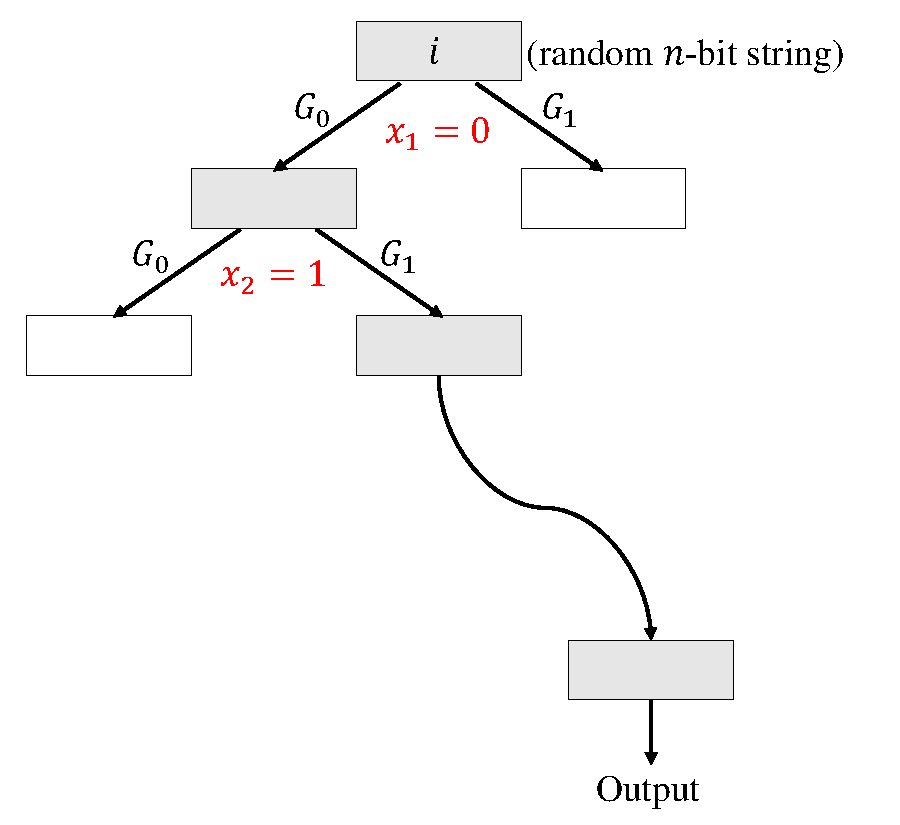
\includegraphics[width=\textwidth]{Old Scribe Notes/binary-tree.pdf}
    \caption{View the construction as a binary tree}
    \label{fig:binary-tree}
\end{marginfigure}

\begin{theorem}\label{theorem:ggm}
The function ensemble $\{F_n\}_{n \in \mathbb{N}}$ constructed above is pseudorandom.
\end{theorem}

\proof
Assume for the sake of contradiction that $\{F_n\}_{n \in \mathbb{N}}$ is not PRG.
Then there exists a non-uniform PPT oracle adversary $\ma$ that can distinguish $\{F_n\}_{n \in \mathbb{N}}$ from $\{R_n\}_{n \in \mathbb{N}}$. Below, via a hybrid argument, we prove that this contradicts the fact that $G$ is a PRG.

Consider the sequence of hybrids $H_i$ for $i \in \{ 0, 1, \cdots, n\}$ where the hybrid $i$ is defined as follows:
\[H_{n,i}^{(K)} (x_1x_2\ldots x_n ):= G_{x_n}(G_{x_{n-1}} (\cdots(G_{x_{i+1}}(K(x_ix_{i-1}\ldots x_1))) \cdots  )), \]
where $K$ is a random function from $\{0,1\}^{i}$ to $\{0,1\}^n$. Intuitively, hybrid $H_i$ corresponds to a binary tree of depth $n$ where the nodes of levels $0$ to $i$ correspond to random values and the nodes at levels $i+1$ to $n$ correspond to pseudorandom values. By inspection, observe that hybrids $H_0$ and $H_n$ are identical to a pseudorandom function and a random function, respectively. There it suffices to prove that hybrids $H_i$ and $H_{i+1}$ are computationally indistinguishable for each $i \in \{ 0, 1, \cdots, n\}$.

We show that $H_{i}$ and $H_{i+1}$ are indistinguishable by considering a sequence of sub-hybrids $H_{i,j}$ for $j \in \{0,\ldots q_{i+1}\}$, where $q_{i+1}$ is the number of the distinct $i-bit$ prefixes of the queries of $\mathcal{A}$.\footnote{Observe that $q_{i+1}$ for each appropriate choice of $i$ is bounded by the running time of $\mathcal{A}$. Hence, this value is bounded by a polynomial in the security parameter.}

We define hybrid $H_{i,j}$ for $j =0$ to be same as hybrid $H_{i}$. Additionally, for $j >0$ hybrid $H_{i,j}$ is defined to be exactly the same as hybrid $H_{i,j-1}$ except the response provided to the attacker for the $j^{th}$ distinct $i-bit$ prefix query of $\mathcal{A}$. Let this prefix be $x^*_n x^*_{n-1} \ldots x^*_{i}$. Note that in hybrid $H_{i,j-1}$ the children of the node $x^*_n x^*_{n-1} \ldots x^*_{i}$ correspond to two pseudorandom values. In hybrid $H_{i,j}$ we replace these two children with random values. By careful inspection, it follows that hybrid $H_{i,q_{i+1}}$ is actually $H_{i+1}$. All we are left to prove is that hybrid $H_{i,j}$ and $H_{i,j+1}$ are indistinguishable for the appropriate choices of $j$ and we prove this below.


Now we are ready to construct an adversary $\mathcal{B}$ that  distinguishes $U_{2n}$ from $G(U_n)$: On input $T \in\{0, 1\}^{2n}$ ($T$ could be either from $U_{2n}$ or $G(U_n)$),
construct a full binary tree of depth $n$ that is exactly the same as $H_{i,j}$ except replacing the children of  $x^*_n x^*_{n-1} \ldots x^*_{i}$ by the value $T$.
Observe that the only difference between $H_{i,j}$ and $H_{i,j+1}$ is that values corresponding to nodes $x_n^*\ldots x_i^* 0$ and $x_n^*\ldots x_i^* 1$ are pseudorandom or random respectively. $\mathcal{B}$ uses the value $T$ to generate these two nodes. Hence success in  distinguishing hybrids $H_{i,j}$ and $H_{i,j+1}$ provides a successful attack for $\mathcal{B}$ in violating security of the pseudorandom generator.
\qed







\section{PRFs from DDH: Naor-Reingold PRF}
We will now describe a PRF function family $F_n: \mathcal{K} \times \{0,1\}^n \rightarrow \mathbb{G}_n$ where DDH is assumed to be hard for  $\{\mathbb{G}_n\}$ and $\mathcal{K}$ is the key space.
The seed for the PRF $F_n$ will be $K =  (h, u_1, \ldots u_n)$, where $u,u_0\ldots u_n$ are sampled uniformly from $|\mathbb{G}_n|$, $g$ is the generator of $\mathbb{G}_n$ and $h = g^u$. 

\[F_n(K,x) = h^{\prod_{i} u_i^{x_i}}\]

Next, we will prove that the function $F_n$ is a pseudo-random function or that $\{F_n\}$ is a pseudo-random function ensemble.\footnote{Here, we require that adversary distinguish the function $F_n$ from a random function from $\{0,1\}^n$ to $\mathbb{G}_n$. Note that the output range of the function is $\mathbb{G}_n$. Note that the distribution of random group elements in $\mathbb{G}_n$ might actually be far from uniformly random strings.}
\begin{lemma}
Assuming the DDH Assumption (see Definition~\ref{def:ddh}) for $\{\mathbb{G}_n\}$ is hard, we have that $\{F_n\}$ is a pseudorandom function ensemble.
\end{lemma}
\begin{proof}
The proof of this lemma is similar to the proof of Theorem~\ref{theorem:ggm}.

Let $R_n^j$ be random function from $\{0,1\}^j \rightarrow \mathbb{G}_n$. Then we want to prove that for all non-uniform PPT adversaries $\mathcal{A}$ we have that:
\[\mu(n) = \left|\Pr[\mathcal{A}^{F_n}(1^n) =1] -  \Pr[\mathcal{A}^{R_n^n}(1^n) =1]\right|\]
is a negligible function. 

For the sake of contradiction, we assume that the function $F_n$ is not pseudorandom. Next, towards a contradiction, we consider a sequence of hybrid functions $F_n^0 \ldots F_n^n$. 
For any $j \in \{0,\ldots n\}$, let $F^j_n((h,u_{j}\ldots u_n),x) = (R_n^j(x_1\ldots x_j))^{\prod_{i=j+1}^n u_i^{x_i}}$, where $R_n^0(\epsilon)$ is the constant function with output $h$. Observe that $F_n^0$ is the same as the function $F_n$ and $F_n^n$ is the same as the function $R_n^n$. Thus, by a hybrid argument, we conclude that there exists $k \in \{0,\ldots n-1\}$, such that 
\[\left|\Pr[\mathcal{A}^{F_n^k}(1^n) =1] -  \Pr[\mathcal{A}^{F_n^{k+1}}(1^n) =1]\right|\]
is a non-negligible function. Now all we are left to show is that this implies an attacker that refutes the DDH assumption. The proof of this claim follows by a sequence of $T$ sub-hybrids, where $T$ is the running time of $\mathcal{A}$. Without loss of generality we assume that $\mathcal{A}$ never makes the same query twice. 

More specifically, we consider a sequence of functions $F_n^{k,t}$ where $t \in \{0,T\}$, $F_n^{k,0}$ is same as $F_n^{k}$ and $F_n^{k,T}$ is same as $F_n^{k+1}$. In particular, we explain how $F_n^{k,t}$ answers queries by $\mathcal{A}$.\footnote{As assumed earlier, keep in mind that $\mathcal{A}$ never makes the same query twice.} Let $x^1, \ldots x^t$ be the first $t$ queries made by $\mathcal{A}$. For any query, $x$ made by $\mathcal{A}$ such that the first $k$ bits of $x$ match the first $k$ bits of one of $x_1, \ldots x_y$ answer as $F_n^{k+1}$ else answer as $F_n^{k}$. Now we can conclude that there exists a $t$ such that $F_n^{k,t}$ and $F_n^{k,t+1}$ are distinguishable with non-negligible probability. 

Finally, we will show that using an adversary that can distinguish between $F_n^{k,t}$ and $F_n^{k,t+1}$ we need to construct an adversary $\mathcal{B}$ that refutes the DDH assumption. We leave construction of this adversary as an exercise.
\end{proof}


\newpage
\section*{Exercises}
\begin{exercise}
\newcommand{\bit}{\{0,1\}}

Prove or disprove: If $f$ is a one-way function, then the following function $B:\bit^*\to\bit$ is a hardconcentrate predicate for $f$. The function $B(x)$ outputs the inner product modulo 2 of the first $\lfloor |x|/2\rfloor$ bits of $x$ and the last $\lfloor |x|/2\rfloor$ bits of $x$.
\end{exercise}

\begin{exercise}
Let $\phi(n)$ denote the first $n$ digits of $\pi = 3.141592653589\ldots$ after the decimal in binary ($\pi$ in its binary notation looks like $11.00100100001111110110101010001000100001\ldots$).

   Prove the following: if one-way functions exist, then there exists a one-way function $f$ such that the function $B:\{0,1\}^* \rightarrow \{0,1\}$ is not a hard concentrate bit of $f$. The function $B(x)$ outputs $\langle x, \phi(|x|)\rangle$, where
    \[\langle a, b\rangle := \sum_{i=1}^n a_i b_i \mod 2\]
    for the bit-representation of $a = {a_1a_2\cdots a_n}$ and $b= {b_1b_2\cdots b_n}$.
\end{exercise}

\begin{exercise}
 If $f: \{0,1\}^{n}\times \{0,1\}^n\rightarrow \{0,1\}^n$  is PRF, then in which of the following cases is $g: \{0,1\}^{n}\times \{0,1\}^n\rightarrow \{0,1\}^n$ also a PRF? \begin{enumerate} \item $g(K,x) = f(K,f(K,x))$ \item $g(K,x) = f(x,f(K,x))$ \item $g(K,x) = f(K,f(x,K))$
    \end{enumerate}
\end{exercise}

\begin{exercise}[Puncturable PRFs.] Puncturable PRFs are PRFs for which a key can be given out such that, it allows evaluation of the PRF on all inputs, except for one designated input.

%\newcommand{\negl}{\mathsf{negl}}
\newcommand{\A}{\mathcal{A}}
\newcommand{\F}{F}
\newcommand{\KeyF}{\mathsf{Key}_{\F}}
\newcommand{\PunctureF}{\mathsf{Puncture}_{\F}}
\newcommand{\EvalF}{\mathsf{Eval}_{\F}}


A puncturable pseudo-random function $\F$ is given by a triple of efficient algorithms ($\KeyF$,$\PunctureF$, and $\EvalF$), satisfying the following conditions:
\begin{itemize}
\item[-] \textbf{Functionality preserved under puncturing}: For every $x^*, x \in \{0,1\}^{n}$ such that $x^* \neq x$, we have that:
    $$\Pr[\EvalF(K,x) = \EvalF(K_{x^*},x) : K \gets \KeyF(1^n), K_{x^*} = \PunctureF(K,x^*)] = 1$$
\item[-] \textbf{Pseudorandom at the punctured point}: For every $x^*\in \{0,1\}^n$ we have that for every polysize adversary $\A$ we have that:
    $$|\Pr[\A(K_{x^*}, \EvalF(K,x^*)) = 1] - \Pr[\A(K_{x^*}, \EvalF(K,U_n)) = 1]|= \negl(n)$$
    where $K \gets \KeyF(1^n)$ and $K_S = \PunctureF(K,x^*)$. $U_n$ denotes the uniform distribution over $n$ bits.
\end{itemize}

Prove that: If one-way functions exist, then there exists a puncturable PRF family that maps $n$ bits to $n$ bits. \\ 
\textbf{Hint:} The GGM tree-based construction of PRFs from a length doubling pseudorandom generator (discussed in class) can be adapted to construct a puncturable PRF. Also note that $K$ and $K_{x^*}$ need not be the same length.
\end{exercise}
%
%\subsection{Application}
%Consider an interesting game: Alice and Bob are talking on the phone.
%Alice flips a coin, and Bob guesses whether it's head or tail.
%But the problem is how can Alice convince Bob that the coin is indeed head or tail?
%If we have pseudorandom functions, the problem could be easily solved.
%
%Assume we have a PRF $F_n: \{0, 1\}^n \rightarrow \{0, 1\}^n$.
%Alice and Bob have a shared key $i \in \{0, 1\}^n$, then $f_i(\cdot)$ is shared information.
%Now Alice has a message $m \in \{0, 1\}^n$ and wants to let Bob guess it,
%the procedure consists of three steps.
%\begin{enumerate}[(a)]
%    \item Alice chooses a string $r \in \{0, 1\}^n$, and sends to Bob  $m' = f_i(r) \oplus m$ ;
%    \item Bob guesses $m$;
%    \item Alice sends $r$ to Bob.
%\end{enumerate}
%In step (a), since $F_n$ is PRF, all the information that Bob gets is a random $n$-bit string, so it will not influence his behavior in step (b).
%Then in step (c), Bob receives $r$ and will be convinced that the true value of $m$ is $f_i(r) \oplus m'$.
%

\chapter{Private-Key Cryptography}
%\newcommand{\key}{\mathsf{k}}
\newcommand{\gen}{\mathsf{Gen}}

\begin{definition}[$\pcnotionstyle{Pri\pcmathhyphen{}}\indcpa$] A private-key encryption scheme $\Pi = (\gen,\enc,\dec)$ is $\pcnotionstyle{Pri\pcmathhyphen{}}\indcpa$-secure if 
$$ \advantage{\indcpa}{\Pi,\adv} = \Large\mid \Pr[\pcnotionstyle{Pri\pcmathhyphen{}}\indcpa_\Pi^\adv(\secpar) =1] -\frac12\Large\mid$$
is a negligible function. 
\end{definition}

\marginnote[-1.5in]{
\procedureblock[linenumbering]{$ \pcnotionstyle{Pri\pcmathhyphen{}}\indcpa_{\Pi}^{\adv}(\secpar)$}{
 b \sample \bin \\
  \key  \sample \gen ( \secparam ) \\
 ( \state ,m_0 ,m_1) \sample \adv^{\enc ( \key ,\cdot )} ( \secparam) \\
 c \sample \enc ( \key ,m_b ) \\
 b' \sample \adv^{\enc ( \key ,\cdot )} ( \state , c ) \\
 \pcreturn b = b' }
 }
\newcommand{\nonnegl}{\mathsf{nonnegl}}


\section{Fixed-length MACs}

Previously, we defined what a MAC is, and specified correctness and security definitions for MACs. In this section, we'll define a fixed-length MAC for length $\ell(n)$.

\begin{theorem}
    If $F : \{0, 1\}^n \to \{0, 1\}^n$ is a PRF, then $\Pi = (\mathsf{Gen}, \mathsf{Mac}, \mathsf{Verify})$ (constructed below) is a MAC, as defined with EF-CMA security.

    \begin{algorithmic}[1]
        \Function{Gen}{$1^n$}
            \State \Return $k \in \{0, 1\}^n$
        \EndFunction
        \Statex
        \Function{Mac}{$k$, $m$}
            \State \Return $F_k(m)$
        \EndFunction
        \Statex
        \Function{Verify}{$k$, $m$, $t$}
            \State \Return $t \overset{?}{=} F_k(m)$
        \EndFunction
    \end{algorithmic}

    That is, we just compute the PRF on our message as the MAC.
\end{theorem}

\begin{proof}
    To prove security, suppose for contradiction that there exists an adversary $A$ that breaks the security for $\Pi$. We'd like to construct an adversary $B$ that breaks the security of the PRF.

    Here, the adversary $A$ expects queries for tags, given messages as input. $B$ can simply forward these requests on to $F$, and return the response back to $A$. Further, $A$ outputs a pair $(m^*, t^*)$, which $B$ can send $m^*$ to $F$, and output whether $t = t^*$.

    \begin{center}
        \begin{tikzpicture}
            \draw (3, 0) rectangle (8, 5.5);
            \draw (5, 0.5) rectangle (7.5, 5);
            \node at (3.25, 5.25) {$B$};
            \node at (5.25, 4.75) {$A$};

            \draw (5.5, 4) edge[->] node[right, pos=0] {$m$} (2.5, 4)
                (2.5, 3.5) edge[->] node[right, pos=1] {$t$} (5.5, 3.5);
            \node[left] at (2.5, 3.75) {$F_k$};
            \node at (5.5, 3.1) {$\vdots$};
            \node at (4.5, 3.1) {$\vdots$};
            \draw (5.5, 2.5) edge[->] node[right, pos=0] {$(m^*, t^*)$} (4.5, 2.5);

            \draw (3.5, 2.5) edge[->] node[right, pos=0] {$m^*$} (2.5, 2.5);
            \node[left] at (2.5, 2.25) {$F_k$};
            \draw (2.5, 2) edge[->] node[right, pos=1] {$t$} (3.5, 2);
            \draw (3.5, 1) edge[->] node[right, pos=0] {$t \overset{?}{=} t^*$} (2.5, 1);
        \end{tikzpicture}
    \end{center}

    Analyzing the probability for $B$, we have
    \[
        \abs{\Pr(B^{F_k(\cdot)}(1^n) = 1) - \Pr(B^{R_n(\cdot)}(1^n) = 1)}
        = \abs{\varepsilon_A(n) - \frac{1}{2^n}}
        = \nonnegl(n)
    .\]
    Here, the first term is because the correctness follows immediately from the correctness of $A$, and the second term is due to the fact that the output of $R_n$ is random.
\end{proof}

\section{Variable-length MACs}

Now, let us look at messages with lengths that are a multiple of $n$. In particular, we have a few blocks $m_1, \ldots, m_{\ell}$, each of size $n$. There are a few ways to do this, but we'll look at a method similar to the counter mode we looked at last time.

\begin{center}
    \begin{tikzpicture}
        \node (m1) at (0, 2) {$m_1$};
        \node (m2) at (1, 2) {$m_2$};
        \node (m3) at (2, 2) {$m_3$};
        \node (mdots) at (3, 2) {$\cdots$};
        \node (ml) at (4, 2) {$m_{\ell}$};

        \node[draw] (fk1) at (0, 0) {$F_k$};
        \node[draw] (fk2) at (1, 0) {$F_k$};
        \node[draw] (fk3) at (2, 0) {$F_k$};
        \node at (3, 0) {$\ldots$};
        \node[draw] (fkl) at (4, 0) {$F_k$};

        \node[outer sep=0pt, inner sep=0pt, draw, circle] (fk1+m2) at (1, 1) {$+$};
        \node[outer sep=0pt, inner sep=0pt, draw, circle] (fk2+m3) at (2, 1) {$+$};
        \node[outer sep=0pt, inner sep=1pt] (xor-dots) at (3, 1) {$\ldots$};
        \node[outer sep=0pt, inner sep=0pt, draw, circle] (dots+ml) at (4, 1) {$+$};

        \draw (m1) edge[->] (fk1)
            (m2) edge[->] (fk1+m2)
            (m3) edge[->] (fk2+m3)
            (ml) edge[->] (dots+ml);

        \draw[->] (fk1) -- ++(0.5, 0) |- (fk1+m2);
        \draw[->] (fk2) -- ++(0.5, 0) |- (fk2+m3);
        \draw[->] (fk3) -- ++(0.5, 0) |- (xor-dots);

        \draw[->] (xor-dots) -- (dots+ml);
        \draw (fk1+m2) edge[->] (fk2)
            (fk2+m3) edge[->] (fk3)
            (dots+ml) edge[->] (fkl);
        \draw (fkl) edge[->] ++(1, 0);
    \end{tikzpicture}
\end{center}

This construction avoids having to store a tag equal in length to the message, but this is not secure, due to length extension attacks. In particular, suppose we query for the tag $t$ associated with $0^n$. We can then query another tag $t'$ for $0^n \oplus t$. Observe here that $t'$ is also the tag for $0^{2n}$.

A solution is to use different keys for each PRF, but this isn't too efficient, since we're still calling the PRF once per block of length $n$. We'll instead improve this to use only one block cipher call---we do some preprocessing and only call $F_k$ once on the output of the preprocessing.

In particular, we'll claim that applying a universal hash function to the input and then applying the block cipher is a secure MAC.

\begin{definition}[Universal Hash Function]
    A function $h : \mathcal{F} \times \mathcal{F}^* \to \mathcal{F}$ (where $\mathcal{F}$ is a field of size $2^m$) is a universal hash function if for all $m, m' \in \mathcal{F}^{\le \ell}$ (i.e. $m$ and $m'$ have length at most $\ell$),
    \[
        \Pr_s(h(s, m) = h(s, m')) \le \frac{\ell}{\abs{F}}
    .\]
    That is, the probability of collision is small.
\end{definition}

Crucially here, we fix $m$ and $m'$, and we sample $s$. (If we fix an $s$, we can almost surely find an $m$ and $m'$ that collide.)

Today, we'll look at the following function:
\[
    h(s, m_0, \ldots, m_{\ell - 1}) = m_0 + m_1 s + m_2 s^2 + \cdots + m_{\ell - 1} s^{\ell - 1} + s^{\ell}
.\]

\begin{claim}
    The function defined by
    \[
        h(s, m_0, \ldots, m_{\ell - 1}) = m_0 + m_1 s + m_2 s^2 + \cdots + m_{\ell - 1} s^{\ell - 1} + s^{\ell}
    \]
    is a universal hash function.
\end{claim}

\begin{proof}
    We'd like to argue that for a fixed $m$ and $m'$, and a random $s$, the probability that there is a collision is at most $\frac{\ell}{\abs{\mathcal{F}}}$.

    We'll look at
    \[
        h(x, m_0, \ldots, m_t) - h(x, m_0', \ldots, m_t') = (m_0 - m_0') + \cdots + (m_{t - 1} - m_{t-1}') x^{\ell - 1}
    .\]
    If there is a collision, this difference is 0. The probability that this polynomial of degree at most $\ell$ has a zero at $x$ is at most $\frac{\ell}{\abs{\mathcal{F}}}$, since it has at most $\ell$ zeroes. This means that $h$ is indeed a universal hash function.
\end{proof}

\begin{claim}
    The MAC given by $F_k(h(s, m_1, \ldots, m_{\ell}))$, for the universal hash function $h$ given prior, is secure. (This is a slight variation on the Carter--Wegman MAC.)
\end{claim}

\begin{proof}
    Suppose for contradiction that there exists a nu-PPT $A$ that breaks the security of this scheme.

    Here, for appropriately generated $k$ and $s$, $A$ makes queries $m \mapsto F_k(h_s(m))$, and outputs $(m^*, t^*)$.

    We'd like to create an adversary $B$ that either breaks the security of the PRF, or breaks the security of the universal hash function.

    $B$ will start by sampling $s \in \mathcal{F}$. When given the query for $m_1$, it computes $h_s(m_1)$ and queries for $F_k(h_s(m_1))$, which it sends back to $A$. If $F_k$ was actually pseudorandom, then $A$ is given a pseudorandom input, and if $F_k$ was random $R_n$, then $A$ is given a random input.

    $A$ must still be able to generate pairs $(m^*, t^*)$ even when given a random input, due to the security of the PRF.

    \begin{center}
        \begin{tikzpicture}
            \draw (2, 0) rectangle (8, 5.5);
            \draw (5, 0.5) rectangle (7.5, 5);
            \node at (2.25, 5.25) {$B$};
            \node at (5.25, 4.75) {$A$};

            \node at (3.5, 4.5) {sample $s \in \mathcal{F}$};

            \node (hsm) at (3.5, 4) {$h_s(m)$};
            \draw (5.5, 4) edge[->] node[right, pos=0] {$m$} (hsm)
                (hsm) edge[->] (1.5, 4)
                (1.5, 3.5) edge[->] node[right, pos=1] {$t$} (5.5, 3.5);
            \node[left] at (1.5, 3.75) {$F_k$};
            \node at (5.5, 3.1) {$\vdots$};
            \node at (4.5, 3.1) {$\vdots$};

            \node (hash-m-star) at (3.5, 2.5) {$h_s(m^*)$};
            \draw (5.5, 2.5) edge[->] node[right, pos=0] {$(m^*, t^*)$} (hash-m-star)
                (hash-m-star) edge[->] (1.5, 2.5);
            \node[left] at (1.5, 2.25) {$F_k$};
            \draw (1.5, 2) edge[->] node[right, pos=1] {$t$} (3.5, 2);
            \draw (3.5, 1) edge[->] node[right, pos=0] {$t \overset{?}{=} t^*$} (1.5, 1);
        \end{tikzpicture}
    \end{center}

    Let $E$ be the event that there exists an $m, m' \in L \cup \{m^*\}$, such that $h_s(m) = h(m')$. If $E$ does not happen, then the hash function never collides. This means that the attacker only sees random values depending on distinct inputs, so this reduces to the case from earlier (when the MAC is just $F_k$).

    As such, we'd like to show that collisions in $h_s(\cdot)$ occur with negligible probability.

    To show this, suppose for contradiction that collisions actually do occur with non-negligible probability. We then want to construct an adversary $B$ utilizing $A$ that just outputs $m$ and $m'$ such that when $s$ is sampled, $h_s(m) = h_s(m')$ with high probability.

    $B$ will pick a random $i, j \in \{1, \ldots, q+1\}$ (here suppose $i < j$), where $q$ is the number of MAC queries. We then run $A$ until the $j$th query. Taking the $i$th and $j$th query, we then output $m_i$ and $m_j$ as our pair of messages. We still need to entertain the queries made by $A$, so we can just return random values for tags (giving the same value if it requests it for the same message).

    \begin{center}
        \begin{tikzpicture}
            \draw (2, 0) rectangle (8, 6);
            \draw (5, 0.5) rectangle (7.5, 5.5);
            \node at (2.25, 5.75) {$B$};
            \node at (5.25, 5.25) {$A$};

            \node[align=center] at (3.5, 5) {\small $i, j \xleftarrow{\$} \{1, \ldots, q+1\}$};

            \draw (5.5, 4) edge[->] node[right, pos=0] {$m_1$} (4.5, 4)
                (4.5, 3.5) edge[->] node[left, pos=0] {sample $t_1$} node[right, pos=1] {$t_1$} (5.5, 3.5);
            \node at (5.5, 3.1) {$\vdots$};
            \node at (4.5, 3.1) {$\vdots$};

            \draw (5.5, 2.5) edge[->] node[right, pos=0] {$m_i$} (4.5, 2.5)
                (4.5, 2) edge[->] node[left, pos=0] {sample $t_i$} node[right, pos=1] {$t_i$} (5.5, 2);
            \node at (5.5, 1.6) {$\vdots$};
            \node at (4.5, 1.6) {$\vdots$};

            \draw (5.5, 1) edge[->] node[right, pos=0] {$m_j$} (4.5, 1);

            \draw (3, 0.5) edge[->] node[right, pos=0] {$(m_i, m_j)$} (1.5, 0.5);
        \end{tikzpicture}
    \end{center}

    By assumption, we know that $E$ occurs with non-negligible probability. That is, among the queries made by $A$, there is a non-negligible probability that $h_s(m_i) = h_s(m_j)$. Since here the implementation of $B$ just picks out a pair of random queries from those made by $A$, the pair $(m_i, m_j)$ output by $B$ also has a collision with non-negligible probability. (In particular, with probability $\Pr(E) / q^2$.

    This breaks the definition of a universal hash function, which is a contradiction.
\end{proof}

So far, we know how to generate tags of fixed length, and of lengths that are a multiple of $n$. If we have a message that is not a multiple of $n$, we could potentially just pad the input with 0's, but this causes an issue, as $m$ and $m \concat 0$ have the same tag.

Instead, one solution is to put the size of the message in the first block, and we can still put the padding at the end. This way, if the messages differ by length, the first block will be different, and if the messages do not differ by length, then we're essentially just ignoring the padding. This gives us a MAC for arbitrary-length messages.

\section{Authenticated Encryption Schemes}

We've talked about confidentiality and integrity separately, but generally we want both properties---when Alice sends a message to Bob, we'd like for any eavesdropper to be unable to recover the message, \emph{and} we'd like Bob to be able to verify that the message actually came from Alice.

A scheme that achieves both of these conditions is called an \emph{authenticated encryption scheme}.

\begin{definition}[Authenticated Encryption Scheme]
    A scheme $\Pi$ is an \emph{authenticated encryption scheme} if it is CPA-secure, and it has ciphertext integrity (CI).
\end{definition}

\begin{definition}[Ciphertext Integrity (CI)]
    Consider the following game for the scheme $\Pi = (\mathsf{Gen}, \mathsf{Enc}, \mathsf{Dec})$.

    \begin{algorithmic}[1]
        \Function{CI${}_{\Pi}^A$}{$n$}
            \State $k \gets \mathsf{Gen}(1^n)$
            \State $c^* \gets A^{\mathsf{Enc}(k, \cdot)}(1^n)$
            \State $L \gets$ the list of queries made by $A$
            \State \Return $(\mathsf{Dec}(k, c^*) \ne \bot) \land (c^* \notin L)$
        \EndFunction
    \end{algorithmic}

    A scheme has ciphertext integrity if for all nu-PPT $A$, $\Pr(\mathrm{CI}_{\Pi}^A)$ is negligible.
\end{definition}

Observe that an authenticated encryption scheme is also CCA-secure, since the CI property says that the adversary can never generate a valid ciphertext. This means that whenever an adversary requests the decryption of a ciphertext, we can always return $\bot$ (unless they previously requested a ciphertext for a message, and wants to decode that ciphertext). This means that the decryption oracle is essentially useless, and this reduces to the CPA case.

Next, we'll construct an authenticated encryption scheme, called ``Encrypt-then-MAC'', utilizing a CPA-secure encryption scheme and an EF-CMA MAC scheme.

\begin{claim}
    Let $\Pi_e = (\mathsf{Gen}_e, \mathsf{Enc}_e, \mathsf{Dec}_e)$ be a CPA-secure encryption scheme, and let $\Pi_m = (\mathsf{Gen}_m, \mathsf{Mac}_m, \mathsf{Verify}_m)$ be an EF-CMA-secure MAC scheme.

    The following scheme $\Pi = (\mathsf{Gen}, \mathsf{Enc}, \mathsf{Dec})$ is an authenticated encryption scheme.

    \begin{algorithmic}[1]
        \Function{Gen}{$1^n$}
            \State $k_e \gets \mathsf{Gen}_e(1^n)$
            \State $k_m \gets \mathsf{Gen}_m(1^n)$
            \State \Return $(k_e, k_m)$
        \EndFunction
        \Statex
        \Function{Enc}{$(k_e, k_m), m$}
            \State $c \gets \mathsf{Enc}_e(k_e, m)$
            \State $t \gets \mathsf{Mac}_m(k_m, c)$
            \State \Return $(c, t)$
        \EndFunction
        \Statex
        \Function{Dec}{$(k_e, k_m), (c, t), m$}
            \If {$\mathsf{Verify}_m(k_m, c, t)$}
                \State \Return $\mathsf{Dec}_e(k_e, c)$
            \Else
                \State \Return $\bot$
            \EndIf 
        \EndFunction
    \end{algorithmic}
\end{claim}

\begin{proof}
    Suppose for contradiction that we have an adversary $A$ that breaks the CPA security of $\Pi$. The CPA game allows for queries of the ciphertext for messages $m$, produces a pair $m_0, m_1$, and then gets $c^* = \mathsf{Enc}(k, m_B)$, and $A$ eventually outputs $b'$ to identify which message was encrypted.

    We'd like to construct another adversary $B$, which breaks the CPA-security of $\Pi_e$. The only difference here is the MACs, so $B$ can sample a $k_m \gets \mathsf{Gen}_m(1^n)$, and perform all of the MACs itself.

    In particular, when $A$ asks for the ciphertext of $M$, we pass it to the oracle for $\Pi_e$, and attach $t \gets \mathsf{Mac}_m(k_m, c)$. If $A$ is able to distinguish between ciphertexts of $M_0$ and $M_1$, then we can use the same bit to distinguish between ciphertexts for $\Pi_e$.
    \begin{center}
        \begin{tikzpicture}
            \draw (1.5, -1) rectangle (8, 6);
            \draw (5, -0.5) rectangle (7.5, 5.5);
            \node at (1.75, 5.75) {$B$};
            \node at (5.25, 5.25) {$A$};

            \node at (3.25, 5) {$k_m \gets \textsc{Gen}_m(1^n)$};

            \node (enc) at (3.25, 3.5) {$C = \textsc{Enc}_e(k_e, m)$};
            \node (mac) at (3.25, 3) {$(C, \textsc{Mac}_m(k_m, C))$};

            \draw (5.5, 4) edge[->] node[right, pos=0] {$m$} (1, 4)
                (1, 3.5) edge[->] (enc)
                (mac) edge[->] node[right, pos=1] {$c$} (5.5, 3);
            \node[left] at (1, 3.75) {$\textsc{Enc}_e(k_e, \cdot)$};
            \node at (5.5, 2.6) {$\vdots$};
            \node at (4.5, 2.6) {$\vdots$};

            \draw (5.5, 2) edge[->] node[right, pos=0] {$m_1, m_2$} node[left, pos=1] {$m_1, m_2$} (1, 2);
            \node (enc-mb) at (3.25, 1.5) {$C^*$};
            \node (mac-mb) at (3.25, 1) {$(C^*, \textsc{Mac}_m(k_m, C^*))$};
            \draw (1, 1.5) edge[->] node[left, pos=0] {$\textsc{Enc}_e(k_e, m_b)$} (enc-mb);
            \draw (mac-mb) edge[->] node[right, pos=1] {$c^*$} (5.5, 1);

            \node at (5.5, 0.5) {$\vdots$};
            \node at (4.5, 0.5) {$\vdots$};

            \draw (5.5, 0) edge[->] node[right, pos=0] {$b'$} (1, 0);
        \end{tikzpicture}
    \end{center}

    To prove ciphertext integrity, suppose we have an adversary $A$ that breaks the ciphertext integrity of $\Pi$. Here, $A$ asks for ciphertext queries, and eventually returns a new ciphertext that is valid.

    We'd like to construct an adversary $B$ that is able to generate a new message and a tag, given oracle access to the MAC scheme. The construction will follow similarly to the prior proof on CPA security.

    Here, our adversary $B$ can sample $k_e \gets \mathsf{Gen}_e(1^n)$. When $A$ asks for the encryption of $M$, $B$ can send $m = \mathsf{Enc}_e(k_e, M)$ to the MAC oracle, and it returns $c = (m, t)$ to $A$.

    When $A$ returns $C^* = (c^*, t^*)$, $B$ can also just return the same, since the tag $t^*$ is being computed on $c^*$.

    \begin{center}
        \begin{tikzpicture}
            \draw (1.5, 1) rectangle (8, 6);
            \draw (5, 1.5) rectangle (7.5, 5.5);
            \node at (1.75, 5.75) {$B$};
            \node at (5.25, 5.25) {$A$};

            \node at (3.25, 5) {$k_e \gets \textsc{Gen}_e(1^n)$};

            \node (enc) at (3.25, 4) {$C = \textsc{Enc}_e(k_e, m)$};
            \node (mac) at (3.25, 3.5) {$T = \textsc{Mac}_m(k_m, C)$};
            \node (enc-mac) at (3.25, 3) {$(C, T)$};

            \draw (5.5, 4) edge[->] node[right, pos=0] {$m$} (enc)
                (enc) edge[->] (1, 4)
                (1, 3.5) edge[->] (mac)
                (enc-mac) edge[->] node[right, pos=1] {$c$} (5.5, 3);
            \node[left] at (1, 3.75) {$\textsc{Mac}_m(k_m, \cdot)$};
            \node at (5.5, 2.6) {$\vdots$};
            \node at (4.5, 2.6) {$\vdots$};

            \node (gen-ciphertext) at (3.25, 2) {$(C^*, T^*)$};
            \draw (5.5, 2) edge[->] node[right, pos=0] {$c^*$} (gen-ciphertext)
                (gen-ciphertext) edge[->] (1, 2);
        \end{tikzpicture}
    \end{center}
\end{proof}

As an example, AES-GCM is the most popular authenticated encryption scheme that is used, and also has the ability to authenticate additional data. (AES-GCM basically just appends the associated data to the ciphertext, so that the encryption is only on the message, but the MAC is on both the ciphertext and the associated data.) This scheme uses a counter-mode encryption scheme, and the MAC that we saw, but makes this more efficient.


% !TEX root = collection.tex

\chapter{Digital Signatures}

In this chapter, we will introduce the notion of a digital signature. At an intuitive level, a digital signature scheme helps providing authenticity of messages and ensuring non-repudiation. We will first define this primitive and then construct what is called as one-time secure digital signature scheme. An one-time digital signature satisfies a weaker security property when compared to digital signatures. We then introduce the concept of collision-resistant hash functions and then use this along with a one-time secure digital signature to give a construction of digital signature scheme.

\section{Definition}

A digital signature scheme is a tuple of three algorithms $(\Gen,\Sign,\Verify)$ with the following syntax:
\begin{enumerate}
\item $\Gen(1^n)\to (vk,sk)$: On input the message length (in unary) $1^n$, $\Gen$ outputs a secret signing key $sk$ and a public verification key $vk$.
\item $\Sign(sk, m) \to \sigma$: On input a secret key $sk$ and a message $m$ of length $n$, the $\Sign$ algorithm outputs a signature $\sigma$.
\item $\Verify(vk, m, \sigma) \to \{0,1\}$: On input the verification key $vk$, a message $m$ and a signature $\sigma$, the $\Verify$ algorithm outputs either $0$ or $1$.
\end{enumerate}

We require that the digital signature to satisfy the following correctness and security properties.\\
\medskip
\noindent\textbf{Correctness.} For the correctness of the scheme, we have that
$\forall m \in \bin^n$,
\[\Pr \left[ (vk,sk) \gets \Gen(1^n), \sigma \leftarrow \Sign(sk,m) : \Verify(vk, m, \sigma) = 1 \right] = 1.\]

\medskip
\noindent\textbf{Security.} Consider the following game between an adversary and a challenger
.

\begin{enumerate}
    \item The challenger first samples $(vk,sk) \gets \Gen(1^n)$. The challenger gives $vk$ to the adversary.
    \item \textbf{Signing Oracle.} The adversary is now given access to a signing oracle. When the adversary gives a query $m$ to the oracle, it gets back $\sigma \gets \Sign(sk,m)$.
    \item \textbf{Forgery.} The adversary outputs a message, signature pair $(m^*,\sigma^*)$ where $m^*$ is different from the queries that adversary has made to the signing oracle.
    \item The adversary wins the game if $\Verify(vk,m^*,\sigma^*) = 1$.
\end{enumerate}
We say that the digital signature scheme is secure if the probability that the adversary wins the game is $\negl(n)$.

\section{One-time Digital Signature}
\label{lampart}
An one-time digital signature has the same syntax and correctness requirement as that of a digital signature scheme except that in the security game the adversary is allowed to call the signing oracle only once (hence the name one-time). We will now give a construction of one-time signature scheme from the assumption that one-way functions exists.

Let $f: \bin^n \rightarrow \bin^n$ be a one-way function.
\begin{itemize}
\item $\Gen(1^n)$: On input the message length (in unary) $1^n$, $\Gen$ does the following:
\begin{enumerate}
    \item Chooses $x_{i,b} \gets \bin^n$ for each $i \in [n]$ and $b \in \bin$.
    \item Output $vk = \left[ \begin{array}{ccc}
f(x_{1,0}) & \ldots & f(x_{n,0}) \\
f(x_{1,1}) & \ldots & f(x_{n,1}) \\
\end{array} \right]$ and $sk = \left[ \begin{array}{ccc}
x_{1,0} & \ldots & x_{n,0} \\
x_{1,1} & \ldots & x_{n,1} \\
\end{array} \right]$
\end{enumerate}
\item $\Sign(sk, m)$: On input a secret key $sk$ and a message $m \in \bin^n$, the $\Sign$ algorithm outputs a signature $\sigma = x_{1,m_1}\|x_{2,m_2}\| \ldots \| x_{n,m_n}$.
\item $\Verify(vk, m, \sigma)$: On input the verification key $vk$, a message $m$ and a signature $\sigma$, the $\Verify$ algorithm does the following:
\begin{enumerate}
    \item Parse $\sigma = x_{1,m_1}\|x_{2,m_2}\| \ldots \| x_{n,m_n}$.
    \item Compute $vk'_{i,m_i} = f(x_{i,m_i})$ for each $i \in [n]$.
    \item Check if for each $i \in [n]$, $vk'_{i,m_i} = vk_{i,m_i}$. If all the checks pass, output 1. Else, output 0.
\end{enumerate}
\end{itemize}

Before we prove any security property, we first observe that this scheme is completely broken if we allow the adversary to ask for two signatures. This is because the adversary can query for the signatures on $0^n$ and $1^n$ respectively and the adversary gets the entire secret key. The adversary can then use this secret key to sign on any message and break the security. 

We will now argue the one-time security of this construction. Let $\adv$ be an adversary who breaks the security of our one-time digital signature scheme with non-negligible probability $\mu(n)$. We will now construct an adversary $\advb$ that breaks the one-wayness of $f$. $\advb$ receives a one-way function challenge $y$ and does the following:
\begin{enumerate}
    \item $\advb$ chooses $i^*$ uniformly at random from $[n]$ and $b^*$ uniformly at random from $\bin$.
    \item It sets $vk_{i^*,b^*} = y$
    \item For all $i \in [n]$ and $b \in \bin$ such that $(i,b) \neq (i^*,b^*)$, $\advb$ samples $x_{i,b} \gets \bin^n$. It computes $vk_{i,b} = f(x_{i,b})$.
    \item It sets $vk = \left[ \begin{array}{ccc}
vk_{1,0} & \ldots& vk_{n,0} \\
vk_{1,1} & \ldots& vk_{n,1} \\
\end{array} \right]$ and sends $vk$ to $\adv$.
\item $\adv$ now asks for a signing query on a message $m$. If $m_{i^*} = b^*$ then $\advb$ aborts and outputs a special symbol $\abort_1$. Otherwise, it uses it knowledge of $x_{i,b}$ for $(i,b) \neq (i^*,b^*)$ to output a signature on $m$.
\item $\adv$ outputs a valid forgery $(m^*,\sigma^*)$. If $m^*_{i^*} = m_{i^*}$ then $\advb$ aborts and outputs a special symbol $\abort_2$. If it does not abort, then it parses $\sigma^*$ as ${1,m_1}\|x_{2,m_2}\| \ldots \| x_{n,m_n}$ and outputs $x_{i^*,b^*}$ as the inverse of $y$.
\end{enumerate}
We first note that conditioned on $\advb$ not outputting $\abort_1$ or $\abort_2$, the probability that $\advb$ outputs a valid preimage of $y$ is $\mu(n)$. Now, probability $\advb$ does not output $\abort_1$ or $\abort_2$ is $1/2n$ (this is because $\abort_1$ is not output with probability $1/2$ and conditioned on not outputting $\abort_1$, $\abort_2$ is not output with probability $1/n$). Thus, $\advb$ outputs a valid preimage with probability $\mu(n)/2n$. This completes the proof of security.

We now try to extend this one-time signature scheme to digital signatures. For this purpose, we will rely on a primitive called as collision-resistant hash functions.

\section{Universal One-way Hash Function -- UOWHF}
We now introduce a class of hash function called universal one-way hash function. 
This form of hash function is stronger than the universal hash function in 4.10 in the sense that the attacker is allowed to select the input by itself but must do so before being presented with the functions description. 

\subsection{Definition}
We now give a formal definition of universal one-way hash function(UOWHF, also called "WOOF"). 
\begin{definition}[Universal One-way Hash Function(UOWHF)]
    Let $\ell$: $\mathbb{N}\rightarrow\mathbb{N}$. A \textit{collection of functions} 
    $\{h_s: \bit^*\rightarrow\bit^{\ell(|s|)}\}_{s\in\bit^{*}}$ is called universal one-way hash functions given $\exists$ PPT machine $I$ such that: 
    \begin{enumerate}
        \item (Easy to compute): $\exists$ a deterministic machine $M$ such that $M(s,x)=h_s(x)$.
        \item (Hard to form designated collisions): Given a PPT attacker $\mathcal{A}$, the probability of $\mathcal{A}$ to win WOOF game is negligible. 
        \[
            \Pr[WOOF^{I,h}_{\mathcal{A}}(n)=1]=\negl
        \]
    \end{enumerate}
\end{definition}
Where $WOOF^{I,h}_{\mathcal{A}}$ is defined in the following:
\begin{enumerate}
    \item $(state, x)\leftarrow\mathcal{A}(1^n)$.
    \item $s\leftarrow I(1^n)$.
    \item $y\leftarrow\mathcal{A}(state, s)$
    \item Output $h_s(x)=h_s(y)$
\end{enumerate}


\subsection{Construction}
We construct UOWHF collections in several steps, starting with a related but
restricted notion and relaxing the restriction gradually until we reach the unrestricted notion of UOWHF collections. 

\begin{definition}[$(d,r)$-UOWHFs]
Let $d,r$: $\mathbb{N}\rightarrow\mathbb{N}$. A \textit{collection of functions} 
    $\{h_s: \bit^{(d(|s|))}\rightarrow\bit^{r(|s|)}\}_{s\in\bit^{*}}$ is called  $(d,r)$-UOWHFs given $\exists$ PPT machine $I$ such that: 
    \begin{enumerate}
        \item $\exists$ a deterministic machine $M$ such that given $s$ and $x\in\bit^{(d(|s|))}$, $M(s,x)=h_s(x)$.
        \item (Hard to form designated collisions): Given a PPT attacker $\mathcal{A}$, the probability of $\mathcal{A}$ to win WOOF game is negligible. 
        \[
            \Pr[WOOF^{I,h}_{\mathcal{A}}(n)=1]=\negl
        \]
    \end{enumerate}
\end{definition}
And $d,r$ satisfying $d(n)>r(n)$. The other case is trivial to discuss. 

Now we discuss the construction of $4$ types of UOWHFs. We start from the simple cases and eventually lead to the full-fledged UOWHFs.

\noindent\textbf{Step I: $(d, d-1)$-UOWHFs}.
We construct UOWHFs that given arbitrary length, truncate its input length by 1. 
\begin{construction}
    Let $f$: $\bit^{*}\rightarrow\bit^{*}$ be a one-way permutation, and $a,b\in GF(2^n)$. We construct $h_s: \bit^{n}\rightarrow\bit^{n-1}$: 
    \[
        h_{s=(a,b)}(x)=chop(a\cdot f(x)+b)
    \]
    where $chop(\cdot)$ is the function that chops the first bit of a given bit string. 
\end{construction}
We then argue that $h_s$ is a $(d,d-1)$-UOWHF. 

\begin{proof}
    We prove this by contradiction. If an adversary $\mathcal{A}$ can break the security of UOWHF, we can construct an adversary $\mathcal{B}$ that breaks the OWF $f$. 

    The algorithm of $\mathcal{B}$ is as follows upon receive an input $y$:
    \begin{enumerate}
        \item $\mathcal{A}$ first emits the preimage $x_0$ of its chosen.
        \item Attacker $\mathcal{B}$ compute $s=(a,b)$ such that $h_s(y)=h_s(x_0)$.
        \item Input $s=(a,b)$ to the oracle $\mathcal{A}$ and output what $\mathcal{A}$ outputs. 
    \end{enumerate}
    
    Since $h_s$ works by chopping the first bit of $af(x)+b$, there are two elements in the preimage of $h_s(x)$, namely $x$ and $x'=f^{-1}(y)$. 
    Because it is easy to compute $a$ and $b$ that $af(x)+b=ay+b$, the hardness relies on finding $x'$ given $y$, which is inverting the one-way permutation. 
    This creates a contradiction of one-way permutation. 
\end{proof}

\noindent\textbf{Step II: $(2n, n)$-UOWHFs}.
Now we construct length-restricted UOWHFs that shrink their input by a factor of 2.

\begin{construction}
    Let $\{h_s: \bit^{*}\rightarrow\bit^{*-1}\}_{s\in\bit^{*}}$. We construct $H_{s_1\cdots s_n}:\bit^{2n}\rightarrow\bit^{n}$:
    \[
        H_{s_1\cdots s_n}=h_{s_1}^{n+1,n}(h_{s_2}^{n+2,n+1}(\cdots h_{s_n}^{2n,2n-1}(x))\cdots)
    \]
\end{construction}
We now prove that $H$ is a $(2n, n)$-UOWHF given $h$ is a $(d,d-1)$-UOWHF.
That is, if we have an attacker $\mathcal{A}$ that can break $(2n, n)$-UOWHF, we can construct an attacker $\mathcal{B}$ that can break the $(d,d-1)$-UOWHF. 
Our intuition is that the attacker $\mathcal{B}$ can randomly inject the challenge $s_i$ into a random location of $S$ to $\mathcal{A}$ and $\mathcal{A}$ will have a non-negligible probability to create a collision. 

\begin{proof}
    Formally we define the procedure of $\mathcal{B}$:
    \begin{enumerate}
        \item Select $i\in [n]$.
        \item $\forall i'\neq i$, sample $s_{i'}$.
        \item Receive $x_0$ from $\mathcal{A}$.
        \item Compute $x_i^0 = H_{partial}(x_0)=h_{s_{n-i+1}}^{2n-i+1,2n-i}(\dots(h_{s_n}^{2n,2n-1}(x))\dots)$, which is the input of i-th hash round select by $\mathcal{B}$
        \item Output $x_0$ to the challenger.
        \item Receive $S_{i}$ from the challenger. And send $\{S_0,\dots,S_n\}$ to $\mathcal{A}$.
        \item $\mathcal{A}$ output $x_1$.
        \item $\mathcal{B}$ compute $H_{partial}(x_1)$ and output.
    \end{enumerate}

The core idea is that if $\mathcal{A}$ can output a collision with different $x$, the output will be the same at some point in the hash chain of applying $h$. 
Therefore $\mathcal{B}$ can randomly insert the challenge into $\mathcal{A}$.
And with $\mu(\mathcal{A})/n$ probability $\mathcal{B}$ will succeed.  $\mu(\mathcal{A})$ is the probability that $\mathcal{A}$ succeed. 
\end{proof}

\noindent\textbf{Step III: UOWHFs that shrinks any input by a factor of two}.

\begin{construction}[(a $(2n^{*}, n^{*})$-UOWHF for any length of $n^{*}$)]
    Let $\{h_s:\bit^{2n}\rightarrow\bit^{n}\}_{s\in\bit^{*}}$. Then for every $x\in\bit^{*}$ we have
    \[
    H_s(x)=h_s(x_1)\cdots h_s(x_{t}10^{n^{*}-|x_t|-1})
    \]
    where $x=x_1\cdots x_t$, $0\leq|x_t|\leq n^{*}$ and $|x_i|=n^{*}$ for $i=1,\dots,t-1$.
\end{construction}

We now give the proof sketch here. 
We want to prove that $H$ is a $(2n^{*}, n^{*})$-UOWHF given $h$ is a $(2n, n)$-UOWHF.
Because $H_s(x)$ is just parallelize $(2n, n)$-UOWHF multiple times. 

We assume that $\mathcal{A}$ is able to create a collision $x'$ for some input $x$ of its given and $s$.
Some block $x'_i$ will be different than the block $x_i$. 
Therefore we have $h_s(x'_i)=h_s(x_i)$ which create contradiction of $h$ is a $(2n, n)$-UOWHF.

\noindent\textbf{Step IV: Full-Fledged UOWHFs}. 
The last step on our way consists of using UOWHFs as constructed in Step III above to obtain
full-fledged UOWHFs.
\begin{construction}[(a UOWHF)]
Let $\{h_s:\bit^{*}\rightarrow\bit^{*}\}_{s\in\bit^{*}}$, such that $|h_s(s)|=|x|/2$, for every $x\in\bit^{2i\cdot|s|}$ where $i\in\mathbb{N}$. Then for every $s_a,\cdots,s_n\in\bit^{n}$, every $t\in\mathbb{N}$ and $x\in\bit^{2^t\cdot n}$, we define
\[
    H_{s_1,\dots,s_n}(x)=(t,h_{s_t}(\cdots(h_{s_2}(h_{s_1}(x)))\cdots))
\]
\end{construction}
The proof is similar in Step II. 

We show how to use the arbitrary-length WOOF we constructed to boost this one-time, fixed-length digital signature scheme into a one-time, arbitrary-length digital signature scheme. 

\subsection{Removing Length-Restriction from One-Time Digital Signatures} 

Let $(\Gen_\ell, \Sign_\ell, \Verify_\ell)$ be a length-restricted one-time digital signature for messages of length $\ell(n)$. 
Let $h_s: \{0,1\}^* \to \{0,1\}^n$ be a WOOF. 
First we will review an \emph{insecure} first attempt at a construction for $\ell(n) = n$: 
\begin{itemize}
    \item $\Gen^{\text{BAD}}(1^n)$: Run $(pk_\ell, sk_\ell) \leftarrow \Gen_\ell(1^n)$, $s \leftarrow I(1^n)$. Output $((pk_\ell,s),sk_\ell)$.

    \item $\Sign^{\text{BAD}}(sk=sk_\ell, m)$: Output $\Sign_\ell(sk_\ell, h_s(m))$. 

    \item $\Verify^{\text{BAD}}(pk=(pk_\ell,s), m, \sigma)$: Output $\Verify_\ell(pk_\ell, h_s(m), \sigma)$. 
\end{itemize}
Notice that this construction does not work because the seed for the WOOF is revealed before the message is chosen, in which case WOOF security does not apply. 

To avoid this, we can use the following construction for $\ell(n) = k(n) + n$ where $k(n)$ is the length of the seed produced by $I(1^n)$: 
\begin{itemize}
    \item $\Gen(1^n)$: Run $(pk_\ell, sk_\ell) \leftarrow \Gen_\ell(1^n)$. Output $(pk_\ell,sk_\ell)$.

    \item $\Sign(sk=sk_\ell, m)$: Run $s \leftarrow I(1^n)$ and $\sigma_\ell \leftarrow \Sign_\ell(sk_\ell, s || h_s(m))$. Output $(\sigma_\ell, s)$. 

    \item $\Verify(pk=pk_\ell, m, \sigma = (\sigma_\ell, s))$: Output $\Verify_\ell(pk_\ell, s || h_s(m), \sigma_\ell)$. 
\end{itemize}
Note that now the seed is chosen after the message. 
We will give a proof sketch of the security for this construction. 
Assume for contradiction that we have a nu-PPT adversary $\adv$ which succeeds with non-negligible probability at the digital signature security game for $(\Gen, \Sign, \Verify)$. 
We will now construct a nu-PPT adversary $\advb$ who succeeds with non-negligible probability at the digital signature security game for $(\Gen_\ell, \Sign_\ell, \Verify_\ell)$, a contradiction. 
$\advb$ receives $pk_\ell$ from its challenger and passes this along to $\adv$. 
When $\adv$ queries the signing oracle with message $m$, $\advb$ runs $s \leftarrow I(1^n)$, computes $m_{\ell} = s || h_{s}(m)$, queries its signing oracle with message $m_{\ell}$ to receive $\sigma_\ell$ and returns $\sigma = (s, \sigma_{\ell})$ to $\adv$. 
Finally, when $\adv$ returns $m^*, \sigma^* = (s^*, \sigma_{\ell}^*)$, $\advb$ outputs $m^*_{\ell} = s^* || h_{s^*}(m^*), \sigma_{\ell}^*$. 

Since we have replicated the expected input distribution for $\adv$, it will succeed with non-negligible probability. 
Notice that $\advb$ will succeed when $\adv$ does as long as $m^*_{\ell} \not = m_{\ell}$. 
In analyzing the success probability of $\advb$ we have two cases to consider based on whether $s^* = s$. 
Notice that $\adv$ must have non-negligible success either when $s^* = s$ or when $s^* \not = s$ or both. 
If $\Pr[s^* \not = s \land \adv \text{ succeeds}]$ is non-negligible, then $\advb$ also succeeds with non-negligible probability since $m^*_{\ell} = s^* || h_{s^*}(m^*) \not = s || h_{s}(m) = m_{\ell}$ in this case. 
Now assume that $\Pr[s^* = s \land \adv \text{ succeeds}]$ is non-negligible. When $\adv$ succeeds in this case, it must have found $m^* \not = m$, and so $h_{s^*}(m^*) = h_{s}(m)$ with only negligible probability because otherwise WOOF security is broken. 
Thus with non-negligible probability $m^*_{\ell} \not = m_{\ell}$ and $\advb$ succeeds as well. 
Therefore either way $\advb$ succeeds in the digital signature game against $(\Gen_\ell, \Sign_\ell, \Verify_\ell)$ with non-negligible probability. 

\section{Multiple-Message Digital Signatures} 

Now we will show how to covert this one-time, no-length restriction digital signature scheme $(\Gen, \Sign, \Verify)$ into a ef-ema no-length restriction digital signature scheme by utilizing a pseudorandom function $PRF$. 
For each $\alpha \in \{\epsilon\} \cup \{0,1\}^{\leq n}$, let $pk_\alpha, sk_\alpha = \Gen(1^n; PRF_s(\alpha 10 \ldots 0))$ such that $|\alpha 10 \ldots 0| = n+1$ (i.e. $\Gen$ is run with randomness determined by the PRF on an input specified by $\alpha$). 
We will use these to make a tree of keys so that the keys used for each message will be distinct with high probability, so WOOF security will continue to apply each time the scheme is used. 
Note that whenever $\Sign$ is called, we require the WOOF to be run with a deterministic seed $s_{\alpha}^W = PRF_{s'}(\alpha 10 \ldots 0)$. 
This way paths through the tree will deterministically map to the corresponding signatures. 
The construction is as follows: 
\begin{itemize}
    \item $\mathsf{GEN}(1^n)$: Output $(pk_\epsilon, s \leftarrow \{0,1\}^n)$, namely the root public key and the seed for the PRF so the rest of the keys can be generated. 

    \item $\mathsf{SIGN}(sk, m)$: 
    \begin{enumerate}
        \item Draw a random path through the key tree $r \leftarrow \{0,1\}^n$. 

        \item Now use the secret key at each level to sign its children's public keys and continue to do this along the random path until a leaf is hit, i.e. iteratively sign the random path and its co-path. 
        Namely, for each $i = 0, 1, \ldots, n-1$, let $\alpha_i = r_1 r_2 \cdots r_i$, $m_i = pk_{\alpha_i || 0} || pk_{\alpha_i || 1}$, and $\sigma_i = \Sign(sk_{\alpha_i}, m_i)$. 

        \item Let $\sigma_n = \Sign(sk_r, m)$. 

        \item Output $\Sigma = (r, m_0, \sigma_0, \ldots, m_{n-1}, \sigma_{n-1}, \sigma_n)$. 
    \end{enumerate} 

    \item $\mathsf{VERIFY}(pk, m, \Sigma = (r, \sigma_0, \ldots, \sigma_{n-1}, \sigma_n))$: Use $r$ and the $m_i$ to determine $pk_{\alpha_i}$ and for each $i \in [n]$ run $\Verify(pk_{\alpha_i}, m_i, \sigma_i)$, accepting if all of those do. 
\end{itemize}
The idea is that because the root $pk_{\epsilon}$ is trusted and the corresponding secret keys of one level are used to validate the $pk$ of the level below, trust is maintained down the path and the ultimate $pk_r$ can be trusted to be used to check the signature on $m$ itself. 

We will now give a proof sketch for the security of this construction. 
Assume for contradiction that we have a nu-PPT adversary $\adv$ which succeeds with non-negligible probability at the digital signature security game for $(\mathsf{GEN}, \mathsf{SIGN}, \mathsf{VERIFY})$. 
Let $\adv$'s interaction with this security game be called Hybrid $H_0$. 
First we will consider the hybrid $H_1$ where the PRF is replaced by a truly random function. 
$\adv$'s success probability in $H_1$ is still some non-negligible $\epsilon(n)$ due to PRF security. 
Now we will consider the hybrid $H_2$ where if the randomness returned by any two of the signing oracle queries is equal, i.e. $r_j = r_{j'}$ for some distinct $j, j' \in [q]$, then $\adv$ aborts. 
Notice that the probability of this happening is only $q^2/2^n$, a negligible amount, so $\adv$'s success probability $\epsilon(n) - q^2/2^n$ remains non-negligible. 
Thus going forward we can assume that the randomness $r_j$ used by the oracle to sign each query $m_j$ is distinct. 

Now notice that either $\adv$ outputs a message-signature pair $(M^*, \Sigma^*)$ which uses $r^* = r_j$ for some $j \in [q]$ or $r^* \not = r_j$ for all $j \in [q]$. 
We will give some intuition for what happens in each of these cases. 
In the first case, since signatures in this scheme are deterministic, to succeed $\adv$'s signatures must be the same as $\Sigma_j$'s along the path $r^* = r_j$ until doing a forgery at the leaf, breaking the $(\Gen, \Sign, \Verify)$ scheme for $M^*$ which is distinct from all of the $m_j$ queries. 
In the second case, $\adv$ goes along a path $r^* \not = r_j$, so at the first node which diverges from all $r_j$ it must forge a signature that verifies with an honest public key from the level above, breaking the $(\Gen, \Sign, \Verify)$ scheme for the corresponding $\alpha_i^*$ which is distinct from all of the other $\alpha_i^j$ that were used to answer queries. 

This can be formalized by constructing a nu-PPT adversary $\advb$ for the one-time digital signature security game of $(\Gen, \Sign, \Verify)$ who takes the $pk$ it's been given and guesses which query $\adv$ forges for, using its $pk$ and one-time oracle to provide a signature for that query and otherwise answering honestly using self-generated keys. 
This degrades $\advb$'s probability of success by $\epsilon(n)/q$ which is still non-negligible. 

Next, after introducing collision resistant hash functions, we will see a different, though closely related, alternate construction for multiple-message digital signatures. 


\section{Collision Resistant Hash Functions}

As the name suggests, collision resistant hash function family is a set of hash functions $H$ such that for a function $h$ chosen randomly from the family, it is computationally hard to find two different inputs $x,x'$ such that $h(x) = h(x')$. We now give a formal definition.

\subsection{Definition of a family of CRHF}

A set of function ensembles
\[ \{H_n = \{h_i : D_n \to R_n \}_{i \in I_n} \}_n\]
where $|D_n| < |R_n|$ is a family of collision resistant hash function ensemble if there exists efficient algorithms $(\Sampler,\Eval)$ with the following syntax:
\begin{enumerate}
\item $\Sampler(1^n) \to i:$ On input $1^n$, $\Sampler$ outputs an index $i \in I_n$.
\item $\Eval(i,x) = h_i(x):$ On input $i$ and $x \in D_n$, $\Eval$ algorithm outputs $h_i(x)$. 
\item $\forall$ PPT $\adv$ we have
\[\Pr[i \gets \Sampler(1^n), (x,x') \gets \adv(1^n,i) : h_i(x) = h_i(x') \wedge x \neq x'] \leq \negl(n)\]
\end{enumerate}


\subsection{Collision Resistant Hash functions from Discrete Log}
We will now give a construction of collision resistant hash functions from the discrete log assumption. We first recall the discrete log assumption:
\begin{definition}[Discrete-Log Assumption]
We say that the discrete-log assumption holds for the group ensemble $\mathcal{G} =\{ \mathbb{G}_n\}_{n \in \mathbb{N}}$, if for every non-uniform PPT algorithm $\mathcal{A}$ we have that
\[\mu_\mathcal{A}(n) := \Pr_{x \leftarrow |G_n|}[\mathcal{A}(g,g^x) = x]\]
is a negligible function.
\end{definition}

We now give a construction of collision resistant hash functions.  

\begin{itemize}
\item $\Sampler(1^n):$ On input $1^n$, the sampler does the following:
\begin{enumerate}
    \item It chooses $x \gets |\mathbb{G}_n|$.
    \item It computes $h = g^x$.
    \item It outputs $(g,h)$.

\end{enumerate}
\item $\Eval((g,h),(r,s)):$ On input $(g,h)$ and two elements $(r,s) \in |\mathbb{G}_n|$, $\Eval$ outputs $g^rh^s$.
\end{itemize}

We now argue that this construction is collision resistant. Assume for the sake of contradiction that an adversary gives a collision $(r_1,s_1) \neq (r_2,s_2)$. We will now use this to compute the discrete logarithm of $h$. We first observe that:
\begin{eqnarray*}
r_1+xs_1 &=& r_2 + xs_2\\
(r_1 - r_2) &=& x(s_2 - s_1)
\end{eqnarray*}
We infer that $s_2 \neq s_1$. Otherwise, we get that $r_1 = r_2$ and hence, $(r_1,s_1) = (r_2,s_2)$. Thus, we can compute $x = \frac{r_1-r_2}{s_1 - s_2}$ and hence the discrete logarithm of $h$ is computable.


\section{CRHF-Based Multiple-Message Digital Signature}

We now explain how to combine collision-resistant hash functions and one-time signatures to get a signature scheme for multiple messages. We first construct an intermediate primitive wherein we will still have the same security property as that of one-time signature but we would be able to sign messages longer than the length of the public-key.\footnote{Note that in the one-time signature scheme that we constructed earlier, the length of message that can be signed is same as the length of the public-key.}


\subsection{One-time Signature Scheme for Long Messages}
We first observe that the CRHF family $H$ that we constructed earlier compresses $2n$ bits to $n$ bits (also called as 2-1 CRHF). We will now give an extension that compresses an arbitrary long string to $n$ bits using a 2-1 CRHF.
\paragraph{Merkle-Damgard CRHF.} The sampler for this CRHF is same as that of 2-1 CRHF. Let $h$ be the sampled hash function. To hash a string $x$, we do the following. Let $x$ be a string of length $m$ where $m$ is an arbitrary polynomial in $n$. We will assume that $m = kn$ (for some $k$) or otherwise, we can pad $x$ to this length. We will partition  the string $x$ into $k$ blocks of length $n$ each. For simplicity, we will assume that $k$ is a perfect power of $2$ or we will again pad $x$ appropriately. We will view these $k$-blocks as the leaves of a complete binary tree of depth $\ell = \log_2 k$. Each intermediate node is associated with a bit string $y$ of length at most $\ell$ and the root is associated with the empty string. We will assign a $\tag \in \bin^n$ to each node in the tree. The $i$-th leaf is assigned $\tag_i$ equal to the $i$-block of the string $x$. Each intermediate node $y$ is assigned a $\tag_y = h(\tag_{y\|0}\| \tag_{y \| 1})$. The output of the hash function is set to be the $\tag$ value of the root. Notice that if there is a collision for this CRHF then there are exists one intermediate node $y$ such that for two different values $\tag_{y\|0},\tag_{y\|1}$ and $\tag'_{y\|0},\tag'_{y\|1}$ we have, $h(\tag_{y\|0},\tag_{y\|1}) = \tag'_{y\|0},\tag'_{y\|1}$. This implies that there is a collision for $h$. 

\paragraph{Construction.} We will now use the Merkle-Damgard CRHF and the one-time signature scheme that we constructed earlier to get a one-time signature scheme for signing longer messages. The main idea is simple: we will sample a $(sk,vk)$ for signing $n$-bit messages and to sign a longer message, we will first hash it using the Merkle-Damgard hash function to $n$-bits and then sign on the hash value. The security of the construction follows directly from the security of the one-time signature scheme since the CRHF is collision-resistant. 

\subsection{Signature Scheme for Multiple Messages}
We will now describe the construction of signature scheme for multiple messages. Let $(\Gen',\Sign',\Verify')$ be a one-time signature scheme for signing longer messages. 
\begin{enumerate}
    \item $\Gen(1^n):$ Run $\Gen'(1^n)$ using to obtain $sk,vk$. Sample a PRF key $K$. The signing key is $(sk,K)$ and the verification key is $vk$.
    \item $\Sign((sk,K),m):$ To sign a message $m$, do the following:
    \begin{enumerate}
        \item Parse $m$ as $m_1m_2\ldots m_{\ell}$ where each $m_i \in \bin$.
        \item Set $sk_0 = sk$ and $m_0 = \epsilon$ (where $\epsilon$ is the empty string).
        \item For each $i \in [\ell]$ do:
        \begin{enumerate}
            \item Evaluate $\PRF(m_1\|\ldots\|m_{i-1}\|0)$ and $\PRF(m_1\|\ldots\|m_{i-1}\|1)$ to obtain $r_0$ and $r_1$ respectively. Run $\Gen'(1^n)$ using $r_0$ and $r_1$ as the randomness to obtain $(sk_{i,0},vk_{i,1})$ and $(sk_{i,1},vk_{i,1})$.
            \item Set $\sigma_i = \Sign(sk_{i-1,m_{i-1}},vk_{i,0}\|vk_{i,1})$
            \item If $i = \ell$, then set $\sigma_{\ell+1} = \Sign(sk_{i,m_i},m)$.
            
        \end{enumerate}
        \item Output $\sigma = (\sigma_1,\ldots,\sigma_{\ell+1})$ along with all the verification keys as the signature.
    \end{enumerate}
    \item $\Verify(vk,\sigma,m)$: Check if all the signatures in $\sigma$ are valid.
\end{enumerate}

To prove security, we will first use the security of the PRF to replace the outputs with random strings. We will then use the security of the one-time signature scheme to argue that the adversary cannot mount an existential forgery.

\section{Trapdoor Permutations and RSA} 

\begin{definition}[Trapdoor Permutation] 
A function family $\{f_s: D_s \to D_s\}_{s \in \{0,1\}^*}$ is a \emph{one-way trapdoor permutation} if there exists PPT $I, D, F, F^{-1}$ such that 
\begin{itemize}
    \item $(s, \tau) \leftarrow I(1^n)$ produces the seed and trapdoor, 
    
    \item $D(s)$ outputs a uniformly random element of $D_s$, 

    \item $\forall s \in I(1^n), x \in D_s$, $F(s, x) = f_s(x)$, 

    \item $\forall (s, \tau) \in I(1^n), y \in D_s$, $F^{-1}(\tau, y) = f_s^{-1}(x)$, and 

    \item $f_s$ is one-way. 
\end{itemize}
\end{definition} 

The RSA trapdoor permutation construction is as follows: 
\begin{itemize} 
    
    \item $I_{RSA}(1^n) \rightarrow (s = (N, e), \tau = (N, d)$ for $N = PQ$ for $2^{n-1} \leq P < Q \leq 2^n$ such that $d = e^{-1} \mod \phi(n)$ for $e < N$ which is coprime to $\phi(n) = (P-1)(Q-1)$. 
    Let $D_s = \{1, \ldots, N\}$. 

    \item $F_{RSA}(s, x) = x^e \mod N$. 

    \item $F_{RSA}^{-1}(\tau, x) = y^d \mod N$. 
\end{itemize}
Unfortunately, under the assumption that factoring is hard, we still don't have a security proof for the RSA trapdoor permutation in the plain model. 
However, we will see a proof in what's called the ``random oracle model'' next. 






\section{Collision Resistant Hash Functions}

As the name suggests, collision resistant hash function family is a set of hash functions $H$ such that for a function $h$ chosen randomly from the family, it is computationally hard to find two different inputs $x,x'$ such that $h(x) = h(x')$. We now give a formal definition.

\subsection{Definition of a family of CRHF}

A set of function ensembles
\[ \{H_n = \{h_i : D_n \to R_n \}_{i \in I_n} \}_n\]
where $|D_n| < |R_n|$ is a family of collision resistant hash function ensemble if there exists efficient algorithms $(\Sampler,\Eval)$ with the following syntax:
\begin{enumerate}
\item $\Sampler(1^n) \to i:$ On input $1^n$, $\Sampler$ outputs an index $i \in I_n$.
\item $\Eval(i,x) = h_i(x):$ On input $i$ and $x \in D_n$, $\Eval$ algorithm outputs $h_i(x)$. 
\item $\forall$ PPT $\adv$ we have
\[\Pr[i \gets \Sampler(1^n), (x,x') \gets \adv(1^n,i) : h_i(x) = h_i(x') \wedge x \neq x'] \leq \negl(n)\]
\end{enumerate}


\subsection{Collision Resistant Hash functions from Discrete Log}
We will now give a construction of collision resistant hash functions from the discrete log assumption. We first recall the discrete log assumption:
\begin{definition}[Discrete-Log Assumption]
We say that the discrete-log assumption holds for the group ensemble $\mathcal{G} =\{ \mathbb{G}_n\}_{n \in \mathbb{N}}$, if for every non-uniform PPT algorithm $\mathcal{A}$ we have that
\[\mu_\mathcal{A}(n) := \Pr_{x \leftarrow |G_n|}[\mathcal{A}(g,g^x) = x]\]
is a negligible function.
\end{definition}

We now give a construction of collision resistant hash functions.  

\begin{itemize}
\item $\Sampler(1^n):$ On input $1^n$, the sampler does the following:
\begin{enumerate}
    \item It chooses $x \gets |\mathbb{G}_n|$.
    \item It computes $h = g^x$.
    \item It outputs $(g,h)$.

\end{enumerate}
\item $\Eval((g,h),(r,s)):$ On input $(g,h)$ and two elements $(r,s) \in |\mathbb{G}_n|$, $\Eval$ outputs $g^rh^s$.
\end{itemize}

We now argue that this construction is collision resistant. Assume for the sake of contradiction that an adversary gives a collision $(r_1,s_1) \neq (r_2,s_2)$. We will now use this to compute the discrete logarithm of $h$. We first observe that:
\begin{eqnarray*}
r_1+xs_1 &=& r_2 + xs_2\\
(r_1 - r_2) &=& x(s_2 - s_1)
\end{eqnarray*}
We infer that $s_2 \neq s_1$. Otherwise, we get that $r_1 = r_2$ and hence, $(r_1,s_1) = (r_2,s_2)$. Thus, we can compute $x = \frac{r_1-r_2}{s_1 - s_2}$ and hence the discrete logarithm of $h$ is computable.


\section{Multiple-Message Digital Signature}

We now explain how to combine collision-resistant hash functions and one-time signatures to get a signature scheme for multiple messages. We first construct an intermediate primitive wherein we will still have the same security property as that of one-time signature but we would be able to sign messages longer than the length of the public-key.\footnote{Note that in the one-time signature scheme that we constructed earlier, the length of message that can be signed is same as the length of the public-key.}


\subsection{One-time Signature Scheme for Long Messages}
We first observe that the CRHF family $H$ that we constructed earlier compresses $2n$ bits to $n$ bits (also called as 2-1 CRHF). We will now give an extension that compresses an arbitrary long string to $n$ bits using a 2-1 CRHF.
\paragraph{Merkle-Damgard CRHF.} The sampler for this CRHF is same as that of 2-1 CRHF. Let $h$ be the sampled hash function. To hash a string $x$, we do the following. Let $x$ be a string of length $m$ where $m$ is an arbitrary polynomial in $n$. We will assume that $m = kn$ (for some $k$) or otherwise, we can pad $x$ to this length. We will partition  the string $x$ into $k$ blocks of length $n$ each. For simplicity, we will assume that $k$ is a perfect power of $2$ or we will again pad $x$ appropriately. We will view these $k$-blocks as the leaves of a complete binary tree of depth $\ell = \log_2 k$. Each intermediate node is associated with a bit string $y$ of length at most $\ell$ and the root is associated with the empty string. We will assign a $\tag \in \bin^n$ to each node in the tree. The $i$-th leaf is assigned $\tag_i$ equal to the $i$-block of the string $x$. Each intermediate node $y$ is assigned a $\tag_y = h(\tag_{y\|0}\| \tag_{y \| 1})$. The output of the hash function is set to be the $\tag$ value of the root. Notice that if there is a collision for this CRHF then there are exists one intermediate node $y$ such that for two different values $\tag_{y\|0},\tag_{y\|1}$ and $\tag'_{y\|0},\tag'_{y\|1}$ we have, $h(\tag_{y\|0},\tag_{y\|1}) = \tag'_{y\|0},\tag'_{y\|1}$. This implies that there is a collision for $h$. 

\paragraph{Construction.} We will now use the Merkle-Damgard CRHF and the one-time signature scheme that we constructed earlier to get a one-time signature scheme for signing longer messages. The main idea is simple: we will sample a $(sk,vk)$ for signing $n$-bit messages and to sign a longer message, we will first hash it using the Merkle-Damgard hash function to $n$-bits and then sign on the hash value. The security of the construction follows directly from the security of the one-time signature scheme since the CRHF is collision-resistant. 

\subsection{Signature Scheme for Multiple Messages}
We will now describe the construction of signature scheme for multiple messages. Let $(\Gen',\Sign',\Verify')$ be a one-time signature scheme for signing longer messages. 
\begin{enumerate}
    \item $\Gen(1^n):$ Run $\Gen'(1^n)$ using to obtain $sk,vk$. Sample a PRF key $K$. The signing key is $(sk,K)$ and the verification key is $vk$.
    \item $\Sign((sk,K),m):$ To sign a message $m$, do the following:
    \begin{enumerate}
        \item Parse $m$ as $m_1m_2\ldots m_{\ell}$ where each $m_i \in \bin$.
        \item Set $sk_0 = sk$ and $m_0 = \epsilon$ (where $\epsilon$ is the empty string).
        \item For each $i \in [\ell]$ do:
        \begin{enumerate}
            \item Evaluate $\PRF(m_1\|\ldots\|m_{i-1}\|0)$ and $\PRF(m_1\|\ldots\|m_{i-1}\|1)$ to obtain $r_0$ and $r_1$ respectively. Run $\Gen'(1^n)$ using $r_0$ and $r_1$ as the randomness to obtain $(sk_{i,0},vk_{i,1})$ and $(sk_{i,1},vk_{i,1})$.
            \item Set $\sigma_i = \Sign(sk_{i-1,m_{i-1}},vk_{i,0}\|vk_{i,1})$
            \item If $i = \ell$, then set $\sigma_{\ell+1} = \Sign(sk_{i,m_i},m)$.
            
        \end{enumerate}
        \item Output $\sigma = (\sigma_1,\ldots,\sigma_{\ell+1})$ along with all the verification keys as the signature.
    \end{enumerate}
    \item $\Verify(vk,\sigma,m)$: Check if all the signatures in $\sigma$ are valid.
\end{enumerate}

To prove security, we will first use the security of the PRF to replace the outputs with random strings. We will then use the security of the one-time signature scheme to argue that the adversary cannot mount an existential forgery.

\section*{Exercises}
\begin{exercise}
\textbf{Digital signature schemes can be made deterministic.} Given a digital signature scheme $(\mathsf{Gen}, \mathsf{Sign}, \mathsf{Verify})$ for which $\mathsf{Sign}$ is probabilistic, provide a construction of a digital signature scheme $(\mathsf{Gen}', \mathsf{Sign}', \mathsf{Verify}')$ where $\mathsf{Sign}'$ is deterministic.
\end{exercise}

% !TEX root = collection.tex

\section{BLS Signatures}

\paragraph{Bilinear Pairings.} Recall that we used prime order groups $\mathbb{G}$ to build the Schnorr signature scheme. Today we will introduce another mathematical object, pairing friendly groups, which support a new ``bilinear pairing'' operation defined as follows. Let $\mathbb{G}_1$, $\mathbb{G}_2$ and $\mathbb{G}_T$ be groups of prime order $p$. We define a bilinear pairing $e: G_1 \times G_2 \rightarrow \mathbb{G}_T$ to be an \emph{efficiently} computable map that satisfies the following properties:
\begin{itemize}
    \item Bilinearity: For all $a, b \in \mathbb{Z}_p$ and $g_1 \in G_1, g_2 \in G_2$, we have $e(g_1^a, g_2^b) = e(g_1, g_2)^{ab}$.
    \item Non-degenerate: $e(g_1, g_2) \neq 1_{\mathbb{G}_T}$.
\end{itemize}
Observe that in any group, by using the group operation, one can compute ``additions'' of the scalar exponents, but in pairing friendly groups one can additionally compute \emph{one} ``multiplication'' of the scalar exponents.

Note that while a pairing provides us with additional \emph{functionality}, it also means that we need to reevaluate any hardness assumptions that we have made. Consider for instance the decisional Diffie-Hellman (DDH) assumption which states that it is hard to distinguish between $(g, g^a, g^b, g^{ab})$ and $(g, g^a, g^b, g^c)$ for random $a, b, c \in \mathbb{Z}_p$. In the presence of a bilinear pairing, natural variants of the DDH assumption are no longer hard such as distinguishing between $(g_1, g_2, g_1^a, g_2^b, g_1^{ab})$ and $(g_1, g_2, g_1^a, g_2^b, g_1^{c})$. Instead, we will define new assumptions that are conjectured to be hard even given a bilinear pairing.

\paragraph{co-CDH assumption.} Let $\mathbb{G}_1$, $\mathbb{G}_2$ be groups of prime order with generators $g_1$ and $g_2$ and let $e: \mathbb{G}_1 \times \mathbb{G}_2 \rightarrow \mathbb{G}_T$ be an efficiently computable bilinear pairing. The co-CDH assumption states that for all non-uniform PPT adversaries $\adv$:
\begin{align*}
    \Pr\left[ \adv(g_1, g_2, g_1^a, g_1^b, g_2^b) \to g_1^{ab} \mid a,b \sample \mathbb{Z}_p \right] \leq \negl
\end{align*}

\paragraph{BLS Signature scheme.} We are now ready to describe the BLS signature scheme~\cite{AC:BonLynSha01}.
\begin{itemize}
    \item $\Gen(1^\lambda)$: Sample $\sk \sample \mathbb{Z}_p$ and set $\vk \gets g_2^\sk$. Output $(\vk, \sk)$.
    \item $\Sign(\sk, m)$: Given a message $m \in \{0,1\}^*$, output $\sigma \gets H(m)^{\sk}$, where $H: \{0,1\}^* \to \mathbb{G}_1$ is a hash function that maps arbitrary strings to elements in $\mathbb{G}_1$.
    \item $\Verify(\vk, m, \sigma)$: Output $e(\sigma, g_2) \stackrel{?}{=} e(H(m), \vk)$.
\end{itemize}

\paragraph{Correctness.} Correctness is easy to see by plugging in explicit expressions for the signature and verification key -- $e(\sigma=H(m)^\sk, g_2) \stackrel{?}{=} e(H(m), \vk=g_2^\sk)$.

\paragraph{Security.} If $H$ is modelled as a random oracle, we will show that if there exists an adversary $\adv$ that can forge a signature with non-negligible probability, then we can use $\adv$ to build $\advb$ that can solve the co-CDH problem with non-negligible probability.

\begin{theorem}
    The BLS signature scheme is is existentially unforgeable under chosen message attacks assuming the co-CDH problem is hard in the random oracle model.
\end{theorem}

\begin{proof}
    We will use a similar strategy as in the proof of RSA full domain hash. Let $\adv$ be a non-uniform PPT adversary that can forge a signature with non-negligible probability. We will use $\adv$ to build a non-uniform PPT adversary $\advb$ that can solve the co-CDH problem with non-negligible probability.
    $\advb$ works as follows:
    \begin{itemize}
        \item $\advb$ receives $(g_1, g_2, g_1^a, g_1^b, g_2^b)$ as input and is tasked with computing $g_1^{ab}$.
        \item $\advb$ now runs the EUF-CMA game with $\adv$ where $\adv$ makes signing queries and in the end outputs a forgery $(m^*, \sigma^*)$, where $m^*$ has not been previously queried.
        \item At the start of the protocol, $\advb$ sets $\vk = g_1^b$ and sends it to $\adv$. For all random oracle queries $H(m)$, $\adv$ samples $r \sample \mathbb{Z}_p$ and sets $H(m) = g_1^r$. When $\adv$ asks for a signature on $m_i$, $\advb$ samples $r_i \sample \mathbb{Z}_p$ and sets $H(m_i) = g_1^{r_i}$ (if the query has not been previously made). It then responds with $\sigma_i = H(m_i)^b = (g_1^b)^{r_i}$. However, for a randomly chosen index $i^*$ (out of the maximum number of queries $\adv$ can make), $\advb$ sets $H(m_{i^*}) = g_1^a$. Now, if $\adv$ asks for a signature on the chosen $m_{i^*}$, $\advb$ aborts and restarts the EUF-CMA game. In the ends, $\adv$ outputs a forgery with non-negligible probability. And since there are only a polynomial number of queries, $\adv$ outputs a forgery on $m_{i^*}$ with non-negligible probability. In which case $\advb$ outputs $\sigma_{i^*}$ as its output in the co-CDH game.
    \end{itemize}

    We now analyze the probability that $\advb$ solves the co-CDH problem.
    \begin{align*}
        \Pr[\advb \to g_1^{ab}] & = \Pr[\adv \text{ outputs forgery} \wedge m_{i^*} \text{ was not queried} \wedge \text{forgery on } m_{i^*}] \\
                                & \geq \epsilon \times \left( 1 -\frac{1}{q_h}\right)^{q_s} \times \frac{1}{q_h}
    \end{align*}
    which is non-negligible.
    Thus, by contradiction, the BLS signature scheme is existentially unforgeable under chosen message attacks assuming the co-CDH problem is hard in the random oracle model.
\end{proof}

\chapter{Public Key Encryption}
Public key encryption allows two parties
to communicate with each other with the guarantees of privacy for their messages against an eavesdropper who monitors all communication between the two parties. Recall that we were able to build Digital Signatures and Symmetric Key Encryption, from the weakest building block in cryptography -- one-way functions. However, there are lower bounds~\cite{STOC:ImpRud89} suggesting that public key encryption cannot be built from one-way functions alone. Instead, we will build public key encryption from more structured assumptions (which are a \emph{stronger} assumption in the sense that they imply one-way functions).

\section{Definitions}
\begin{definition}[Public Key Encryption]
    A public key encryption scheme is a tuple of three algorithms $(\gen$, $\enc, \dec)$ defined as follows:
    \begin{itemize}
        \item $\gen(1^\secpar) \to (\pk, \sk)$: outputs a public key and secret key $(\pk, \sk)$.

        \item $\enc(\pk, m) \to c$: Takes as input the public key and a message $m$ and outputs a ciphertext $c$.

        \item $\dec(\sk, c) \to m$: Takes as input a secret key $\sk$ and ciphertext $c$, and output a message $m$.
    \end{itemize}
\end{definition}

\begin{definition}[Perfect Correctness]
    A public key encryption scheme $(\gen$, $\enc, \dec)$ is said to be correct if for all $\secpar \in \mathbb{N}$, $(\pk, \sk) \gets \gen(1^\secpar)$, $m \in \{0,1\}^*$, it holds that
    \[\Pr[\dec(\sk, \enc(\pk, m)) = m] = 1\]
\end{definition}
The above definition can be relaxed to allow for a negligible probability of error during decryption and still remain meaningful.

We now define two different notions of security for public key encryption schemes -- IND-CPA and IND-CCA security.
\begin{definition}[IND-CPA Security]
    A public key encryption scheme $(\gen$, $\enc, \dec)$ is said to be IND-CPA-secure if for all non-uniform PPT $\adv$,
    \[\left|\Pr[\mathsf{Exp}_{\adv}^{\mathsf{CPA}(\secpar)} = 1] - \frac{1}{2}\right| \leq \negl,\]
    where $\mathsf{Exp}_{\adv}^{\mathsf{CPA}(\secpar)}$ is defined as follows:
    \begin{itemize}
        \item $(\pk, \sk) \gets \gen(1^\secpar)$.
        \item $b \sample \{0,1\}$.
        \item $\adv(\pk) \to (m_0, m_1, \mathsf{st})$.
        \item $c^* \gets \enc(\pk, m_b)$.
        \item $\adv(c^*, \mathsf{st}) \to b'$.
        \item Output $1$ if $b = b'$ and $0$ otherwise.
    \end{itemize}
\end{definition}

\begin{definition}[IND-CCA Security]
    A public key encryption scheme $(\gen$, $\enc, \dec)$ is said to be IND-CCA-secure if for all non-uniform PPT $\adv$,
    \[\left|\Pr[\mathsf{Exp}_{\adv}^{\mathsf{CCA}(\secpar)} = 1] - \frac{1}{2}\right| \leq \negl,\]
    where $\mathsf{Exp}_{\adv}^{\mathsf{CCA}(\secpar)}$ is defined as follows:
    \begin{itemize}
        \item $(\pk, \sk) \gets \gen(1^\secpar)$.
        \item $b \sample \{0,1\}$.
        \item $\adv^{\Dec(\sk)}(\pk) \to (m_0, m_1, \mathsf{st})$.
        \item $c^* \gets \enc(\pk, m_b)$.
        \item $\adv^{\Dec(\sk)}(c^*, \mathsf{st}) \to b'$, where the decryption oracle now returns $\bot$ when queried on $c^*$.
        \item Output $1$ if $b = b'$ and $0$ otherwise.
    \end{itemize}
\end{definition}

\section{Trapdoor Functions}
\begin{definition}[Trapdoor Function]
    A trapdoor function is a tuple of four algorithms $(\gen, f, f^{-1}, D)$ defined as follows:
    \begin{itemize}
        \item $\gen(1^\secpar) \to (s,t)$: outputs an index $s$ and corresponding trapdoor $t$.
        \item $D(s)$: Outputs a description of the domain of the trapdoor function.
        \item $f(s, x) \to y$: Takes as input an index $s$ and a element $x$ from the domain of the trapdoor function and outputs an element $y$.
        \item $f^{-1}(t, y) \to x$: Takes as input a trapdoor $t$ and an element $y$ from the range of the trapdoor function and outputs an element $x$.
    \end{itemize}
    We require the following properties:
    \begin{itemize}
        \item \textbf{Correctness:} For all $\secpar \in \mathbb{N}$, $(s,t) \gets \gen(1^\secpar)$, $x \in D(s)$, it holds that $\Pr[f^{-1}(t, f(s, x)) \neq x] = \negl$. Note that if we demand that $f$ is injective, then this property is automatically satisfied.
        \item \textbf{One-wayness:} For all non-uniform PPT $\adv$, we have $\Pr[\adv(s, y) \to x \mid (s,t) \gets \gen(1^\secpar), x \sample D(s), y \gets f(s, x)] = \negl$.
    \end{itemize}
\end{definition}

\section{Public Key Encryption from Trapdoor Functions}
Given a trapdoor function, we can build a public key encryption scheme as follows:
\begin{itemize}
    \item $\gen(1^\secpar)$: Run $\mathsf{TDF}.\gen(1^\secpar)$ to obtain $(s,t)$. Set $\pk = s$ and $\sk = t$.
    \item $\enc(\pk, m)$: Sample $x \sample D(s)$ and compute $y \gets f(s, x)$. Sample $r \sample \{0,1\}^{|x|}$ and output $c = (y, r, m \oplus \mathsf{HC}(x,r))$, where $\mathsf{HC}$ is the hardness concentration bit, as defined in~Section~\ref{sec:levin-owf}.
    \item $\dec(\sk, c)$: Parse $c = (y, r, z)$ and output $m = z \oplus \mathsf{HC}(f^{-1}(t, y), r)$.
\end{itemize}

\paragraph{Proof Sketch.} To show that the above scheme is CPA secure, observe that the message space $\{0,1\}$. So the only two messages the distinguisher can pick are $m_0=0$ and $m_1=1$. Now if the distinguisher can indeed distinguish between encryptions of $m_0$ and $m_1$, then the same distinguisher can be used to identify the hardness concentration bit. By using a similar strategy as in the proof of~Theorem~\ref{thm:hard-concentrate-bit}, we can recover the pre-image $x$ of the trapdoor function. Thus, violating the one-wayness of the trapdoor function.

\section{Public Key Encryption from Computational Diffie-Hellman}
Although we have a construction of public key encryption from trapdoor functions, we did not know how to build trapdoor functions from some very natural assumptions such as CDH for quite some time. It was only recently that Garg and Hajiabadi~\cite{C:GarHaj18} showed that this was indeed possible. Given the non-trivial nature of the construction, we will not cover it in this course and instead provide a \emph{direct} construction of public key encryption from the Computational Diffie-Hellman (CDH) assumption.

Let $\mathbb{G}$ be a prime order group of order $p$ with generator $g$, where the CDH problem is assumed to be hard.
\begin{itemize}
    \item $\gen(1^\secpar)$: Sample $\sk \sample \mathbb{Z}_p$ and set $\pk \gets g^\sk$. Output $(\pk, \sk)$.
    \item $\enc(\pk, m)$: Sample $\alpha \sample \mathbb{Z}_p$, and set $y \gets g^\alpha$, $k \gets \pk^\alpha$. Now sample $r \sample \{0,1\}^{|B|}$ and output $c = (y, r, m \oplus \mathsf{HC}(k, r))$.
    \item $\dec(\sk, c)$: Parse $c = (y, r, z)$ and compute $k \gets y^\sk$. Output $m = z \oplus \mathsf{HC}(k, r)$.
\end{itemize}

\paragraph{Proof Sketch.} The proof of security is similar to the proof of security for the trapdoor function based public key encryption scheme. The only difference is that we now we reduce the hardness of the CDH problem.

\section{Improving Efficiency.}
The above construction can only be used to encrypt a single bit and results in a ciphertext of size $O(\poly)$. Encrypting a message with $M$ bits, results in a ciphertext of size $O(M \cdot \poly)$. Encryption and decryption also requires $O(M)$ public-key operations (evaluating the TDF/group operations) and we would like to bring this down to $O(1)$. The idea is to extract a symmetric key instead of a single bit by replacing the hardness concentration function with a random oracle. We can then use the symmetric key to encrypt long message with constant rate.

The construction is almost identical except that we replace the hardness concentration bit with a random oracle to extract a symmetric key that can be used to encrypt a long message. Given a trapdoor function the construction works as follows:
\begin{itemize}
    \item $\gen(1^\secpar)$: Run $\mathsf{TDF}.\gen(1^\secpar)$ to obtain $(s,t)$. Set $\pk = s$ and $\sk = t$.
    \item $\enc(\pk, m)$: Sample $x \sample D(s)$ and compute $y \gets f(s, x)$. Encrypt $m$ using a symmetric encryption scheme with key $H(x)$ as $z \gets \mathsf{Sym}.\enc(H(x), m)$. Output $c = (y, z)$.
    \item $\dec(\sk, c)$: Parse $c = (y, z)$ and compute $x \gets f^{-1}(t, y)$. Decrypt $z$ using the symmetric encryption scheme with key $H(x)$ as $m \gets z \oplus \mathsf{Sym}.\dec(H(x), z)$. Output $m$.
\end{itemize}


\section{Fujisaki-Okamoto Transformation}


\section{Post-Quantum Public Key Encryption}
The public-key encryption schemes discussed so far, rely on the difficulty of problems like factorization or discrete logarithms. In 1994, Peter Shor showed that these problems can be solved efficiently on a quantum computer~\cite{FOCS:Shor94}. Even though we do not have large-scale quantum computers capable of breaking current encryption schemes, there are two reasons to begin the transition of public-key encryption to quantum-resistant schemes:
\begin{itemize}
    \item Encrypted messages captured today can be stored and decrypted in the future when a large scale quantum computer is available. This is commonly referred to as the "harvest now, decrypt later" risk.
    \item Transition to new encryption schemes is a slow process and it is important to start the transition well before large scale quantum computers are available.
\end{itemize}

The national institute of standards and technology (NIST) opened a call for post-quantum public-key encryption and signature schemes in 2016. In Nov 2019, it received 59 submissions for public-key encryption and 23 submissions for digital signatures. In July 2022, NIST announced the first batch of winners for public-key encryption and digital signatures. In Aug 2024, the final standard for these schemes was published and they are now making their way into existing infrastructure. There was one winner (CRYSTALS-Kyber) for public-key encryption (based on lattices) and three winners for digital signatures (two based on lattices and one based on hash functions).

\begin{figure}[!htbp]
    \begin{tikzpicture}[node distance=1.5cm and 2cm,
            every node/.style={align=center}, % Adjust width as needed
            >=stealth] % Nicer arrow tips
        \node[align=center](lwe) {LWE \\ \cite{STOC:Regev05}};
        \node[right=of lwe] (lweske) {LWE-SKE};
        \node[right=of lweske, align=center] (lwepke) {LWE-PKE \\ \cite{STOC:Regev05} \\ LWE + LHL };
        \node[right=of lwepke, align=center] (comlwepke) {Compact LWE-PKE \\ \cite{RSA:LinPei11} \\ LWE + LWE};
        \node[below=of lweske, align=center] (rlwe) {RLWE \\ \cite{EC:LyuPeiReg10}};
        \node[right=of rlwe, align=center] (rlwepke) {RLWE-PKE \\ \cite{EC:LyuPeiReg13} \\ RLWE + RLWE};
        \node[below=of rlwe, align=center] (mlwe) {MLWE \\ \cite{ITCS:BraGenVai12,DCC:LanSte15}};
        \node[below=of comlwepke, align=center] (kyber) {CRYSTALS-Kyber \\ MLWE + MLWE};

        \draw[->] (lwe) -- (lweske);
        \draw[->] (lweske) -- (lwepke);
        \draw[->] (lwepke) -- (comlwepke);
        \draw[->] (lwe) -- (rlwe);
        \draw[->] (lwe) -- (mlwe);
        \draw[->] (rlwe) -- (rlwepke);
        \draw[->] (comlwepke) -- (rlwepke);
        \draw[->] (mlwe) -- (kyber);
        \draw[->] (comlwepke) -- (kyber);
        \draw[->] (rlwepke) -- (kyber);
        % Bounding box
        % \draw[dashed, thick] ($(lwe.north west)+(-0.5,0.5)$) rectangle ($(kyber.south east)+(0.5,-3)$);
    \end{tikzpicture}
    \caption{A roadmap of lattice-based public-key encryption schemes ending in the standardized CRYSTALS-Kyber scheme.}
\end{figure}


\begin{definition}[Learning With Errors Assumption (Search)]
    Let $m,n,q \in \mathbb{N}$ and $\chi$ be a distribution over $\mathbb{Z}_q$. The Learning With Errors (LWE) $\LWE_{n,m,q,\chi}$ problem is defined as follows:
    \[\Pr[\adv(A,b) \to s \mid s \sample \mathbb{Z}_q^n, A \sample \mathbb{Z}_q^{m \times n}, b = A \cdot s + e ] \leq \negl\]
\end{definition}

\begin{definition}[Learning With Errors (Decision)]
    Let $m,n,q \in \mathbb{N}$ and $\chi$ be a distribution over $\mathbb{Z}_q$. The Learning With Errors (LWE) $\LWE_{n,m,q,\chi}$ problem is defined as follows:
    \begin{multline*}
        |\Pr[\adv(A,b) \to 1 \mid s \sample \mathbb{Z}_q^n, A \sample \mathbb{Z}_q^{m \times n}, b = A \cdot s + e ] \\
        - \Pr[\adv(A,b) \to 1 \mid s \sample \mathbb{Z}_q^n, A \sample \mathbb{Z}_q^{m \times n}, b \sample \mathbb{Z}_q^m ]|\leq \negl
    \end{multline*}
\end{definition}
The Learning With Errors assumption is commonly referred to as a Lattice based assumption because there is a reduction from Search/Decision LWE to a ``worst-case'' lattice problem.

The above assumptions have been stated with respect to some abstract distribution $\chi$ over $\mathbb{Z}_q$. But what do we actually choose this distribution to be? In the extreme case of $\chi = 0$, the LWE problem is trivial as one can simply use Gaussian Elimination. In the other extreme if $\chi$ is uniform over $\mathbb{Z}_q$, then the LWE problem is information theoretically hard (but not very useful for cryptography). We will be interested in the intermediate case where $\chi$ is a \emph{small} distribution over $\mathbb{Z}_q$, centered around 0. For eg: $\chi$ is a uniform distribution over $[-B, B]$ for some $B \ll q/2$. This will allow us to do build interesting cryptographic primitives like public key encryption and signature schemes. For provable reductions to lattice problems, we set $\mathsf{stddev}(\chi) = \Omega(\sqrt{n})$. However, there is a gap between the best known attacks on LWE and the best known reductions to lattice problems. As a result, much more aggressive parameters are used in practice, chosen based on the best known attacks. Typical parameters for LWE are $n = 512$, $q = 3329$, $\mathsf{supp}(\chi) = [-3,3]$, and $m = 768$. \cite{EPRINT:AlbPlaSco15} provides a lattice estimator \url{https://github.com/malb/lattice-estimator} that can be used to estimate the number of bits of security provided by a given set of LWE parameters.

\subsection{LWE $\to$ LWE-SKE}
As a first step, we will see how to build a symmetric key encryption scheme from LWE.

\begin{itemize}
    \item $\Gen$: Sample $s \sample \mathbb{Z}_q^n$ and output $\sk = s$.
    \item $\Enc(\sk,\mu)$: Sample $a \sample \mathbb{Z}_q^n$, $e \sample \chi$, and compute $b \gets \langle a, s \rangle + e$. Output $c = (c_0 = a, c_1 = b + \lfloor\frac{q}{2}\rfloor\mu)$.
    \item $\Dec(\sk,c)$: Parse $c = (c_0, c_1)$ and compute $m \gets \mathsf{Decode}(c_1 - \langle c_0, s \rangle)$, where $\mathsf{Decode}(\hat{\mu}) \to \{0,1\}$ takes a value from $\mathbb{Z}_q$ and outputs $0$ if $\hat{\mu}$ is closer to $0$ than to $\lfloor\frac{q}{2}\rfloor$ and $1$ otherwise.
\end{itemize}

\begin{theorem}
    If the decisional variant of LWE is hard, then the above scheme is a secure symmetric key encryption scheme.
\end{theorem}
\begin{proof}
    Let the ciphertext $c = (c_0, c_1)$. Then $\hat{\mu} = c_1 - \langle c_0,s\rangle = b + \lfloor\frac{q}{2} - \langle a,s\rangle = \lfloor\frac{q}{2}\rfloor\mu + e$.

\end{proof}
\section{Cramer-Shoup Construction}

\chapter{Advanced Encryption Schemes}
\section{Identity-Based Encryption}

We introduce Bilinear Maps and two of its applications: NIKE, Non-Interactive Key Exchange; and IBE, Identity Based Encryption.


\section{Diffie-Hellman Key Exchange}

\begin{figure}
\label{fig:dh}
\centering
  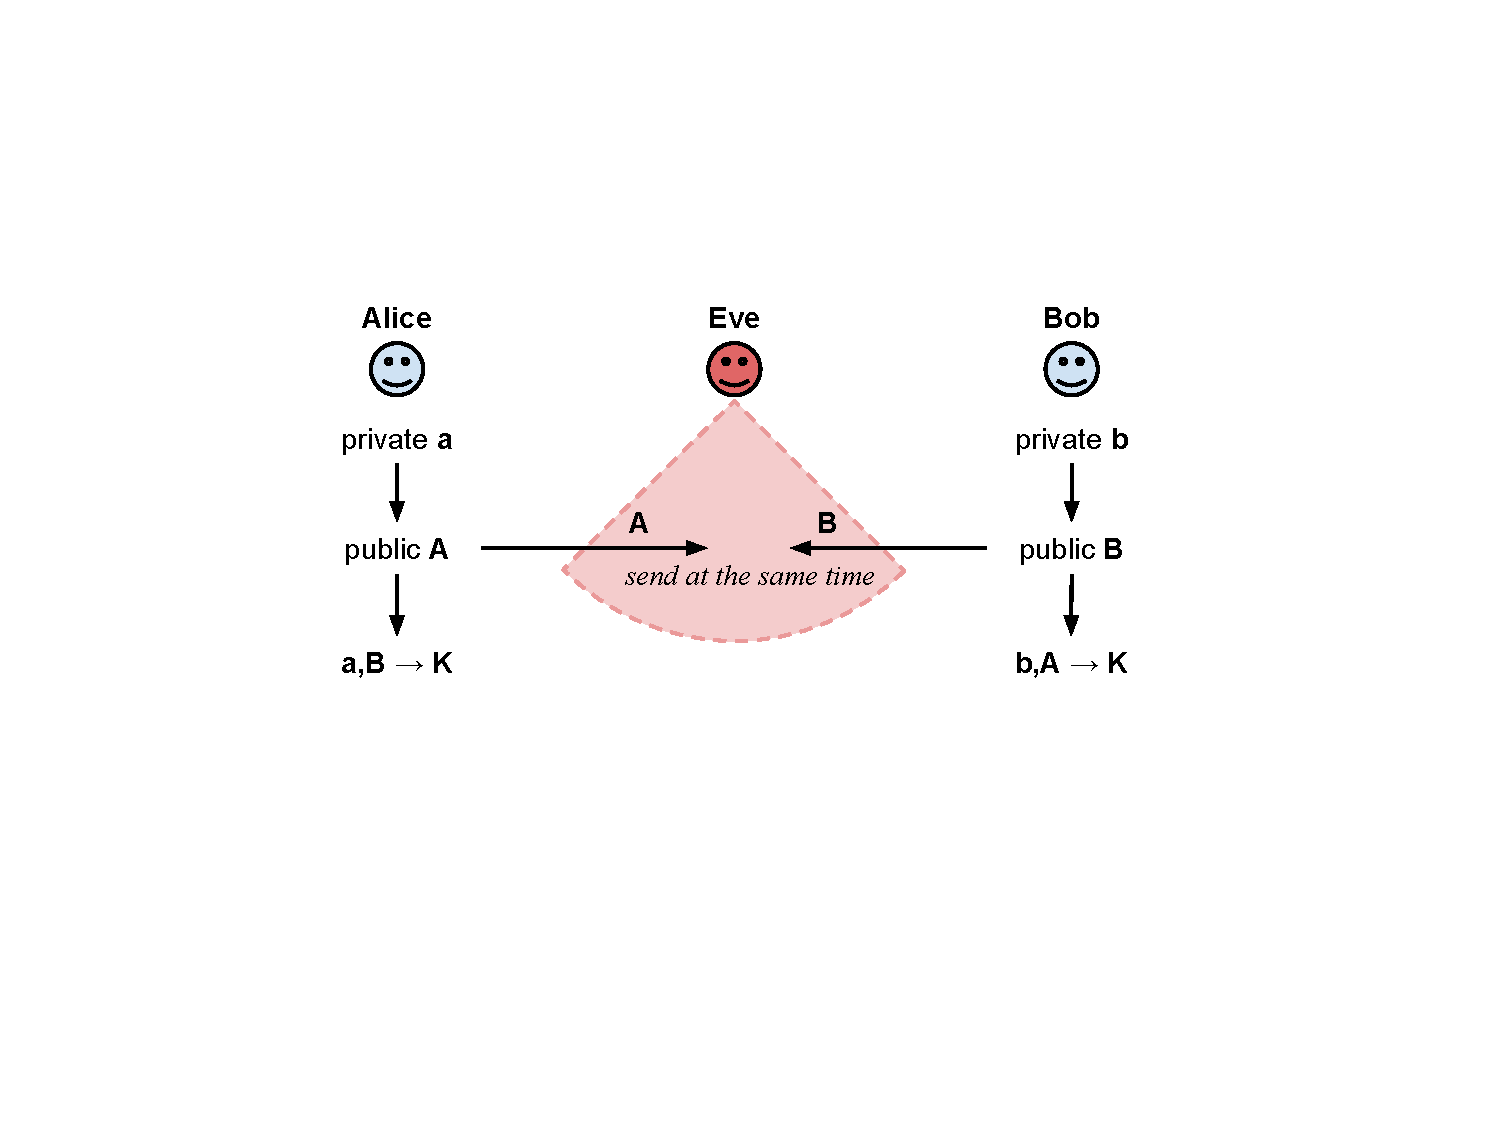
\includegraphics[width=0.7\textwidth]{Old Scribe Notes/fig1.pdf}
\caption{Diffie-Hellman Key Exchange}
\end{figure}


Fig \ref{fig:dh} illustrates Diffie-Hellman key exchange. Alice and Bob each has a private key ($a$ and $b$ respectively), and they want to build a shared key for symmetric encryption communication. They can only communicate over a insecure link, which is eavesdropped by Eve.
So Alice generates a public key $A$ and Bob generates a public key $B$, and they send their public key to each other at the same time. Then Alice generates the shared key $K$ from $a$ and $B$, and likewise, Bob generates the shared key $K$ from $b$ and $A$.
And we have $\forall$ PPT Eve, $Pr[k=Eve(A,B)]=neg(k)$, where $k$ is the length of $a$.


\subsection{Discussion 1}

Assume that $\forall (g, p)$, and $a_1,b_1 \stackrel{\$}{\gets} Z^*_p$, and $a_2,b_2,r \stackrel{\$}{\gets}Z^*_p$, we have $(g^{a_1}, g^{b_1}, g^{a_1b_1}) \stackrel{c}{\simeq} (g^{a_2}, g^{b_2}, g^r)$. How to apply this to Diffie-Hellman Key Exchange?


Make $A=g^a$, $B=g^b$, $K=A^b=g^{ab}$, and $K=B^a=g^{ab}$.


\subsection{Discussion 2}


How does Diffie-Hellman Key Exchange imply Public Key Encryption?


Alice
$pk = A$, $sk = a$, $Enc(pk, m \in \{0, 1\})$.

Bob
$b,r \gets Z^*_p$
$(g^b, mA^b+(1-m)g^r)$

Alice $Dec(sk, (c_1, c_2))$

$c_1^a \stackrel{?}{=} c_2$




\section{Bilinear Maps}

\begin{definition}{Bilinear Maps}

Bilinear Maps is $(G,P,G_T,g,e)$, where $e$ is an efficient function $G \times G \to G_T$ such that

\begin{itemize}
\item if $g$ is generator of $G$, then $e(g, g)$ is the generator of $G_T$.
\item $\forall a,b \in Z_p$, we have $e(g^a, g^b) = e(g, g)^{ab} = e(g^b, g^a)$.
\end{itemize}

\end{definition}

\subsection{Discussion 1}


How does Bilinear Maps apply to Diffie-Hellman?

Make $A=g^a$, $B=g^b$, and $T=g^{ab}$, then Diffie-Hellman has $e(A, B)=e(g, T)$.


\section{Tripartite Diffie-Hellman}

\begin{figure}
\label{fig:3dh}
\centering
  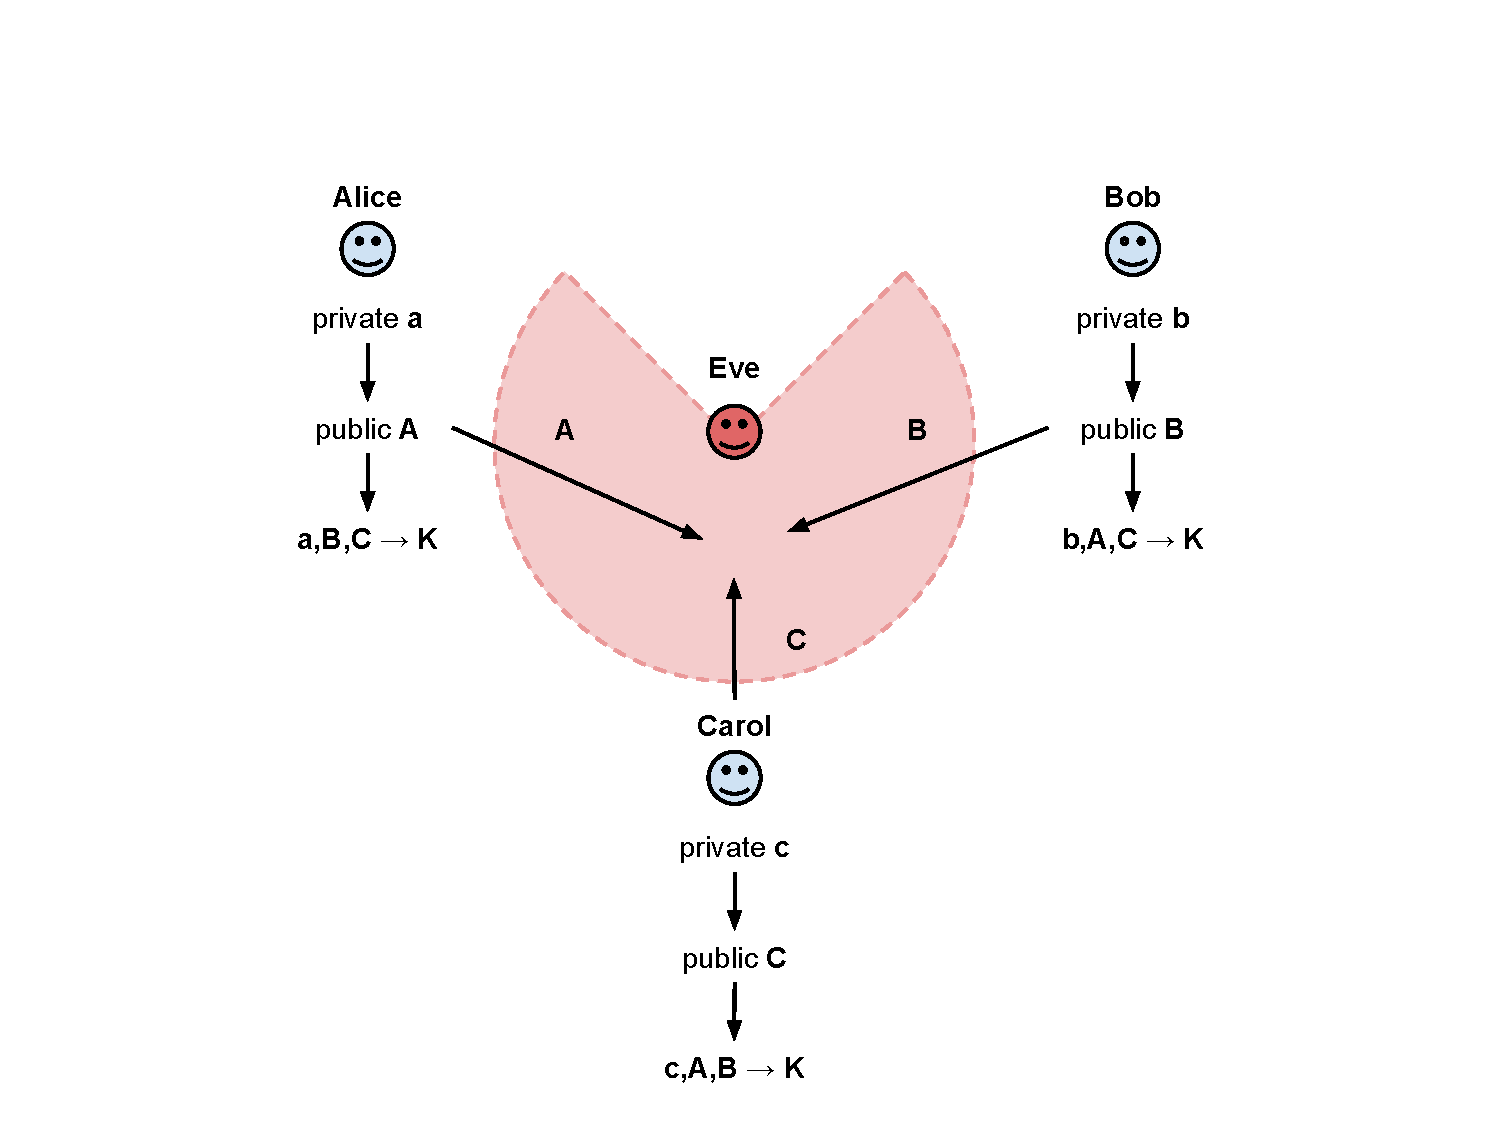
\includegraphics[width=0.7\textwidth]{Old Scribe Notes/fig2.pdf}
\caption{Tripartite Diffie-Hellman Key Exchange}
\end{figure}

Fig \ref{fig:3dh} illustrates Tripartite Diffie-Hellman key exchange. $a$, $b$, and $c$ are private key of Alice, Bob, and Carol, respectively.
They use $g^a$, $g^b$, $g^c$ as public key, and the shared key $K=e(g,g)^{abc}$.
Formally, we have
$$a,b,c \stackrel{\$}{\gets} Z^*_p, r \stackrel{\$}{\gets} Z^*_p$$
$$A=g^a, B=g^b, C=g^c$$
$$K=e(g,g)^{abc}$$



\section{IBE: Identity-Based Encryption}
IBE contains four steps: \emph{Setup}, \emph{KeyGen}, \emph{Enc}, and \emph{Dec}. We illustrate it in Figure \ref{fig:ibe}.
In first step, Key authority get a Master Public Key (MPK) and Master Signing Key (MSK) from $Setup(1^k)$. Then a user with an ID
 (in this example, ``Mike''), sends his ID to the key authority. The key authority generates the Signing Key of Mike with $KeyGen(MSK, ID)$ ans sends it back. Another use, Alice, wants to send an encrypted message to Mike. She only has MPK and Mike's ID. So she encrypts the message with $c=Enc(MPK, ID=Mike, m)$, and sends the encrypted message $c$ to Mike. Mike decodes $c$ with $m=Dec(c, SK_{Mike})$. Notice that Alice never need to know Mike's public key. She only needs to remember MPK and other people's IDs.

\begin{figure}
\label{fig:ibe}
\centering
  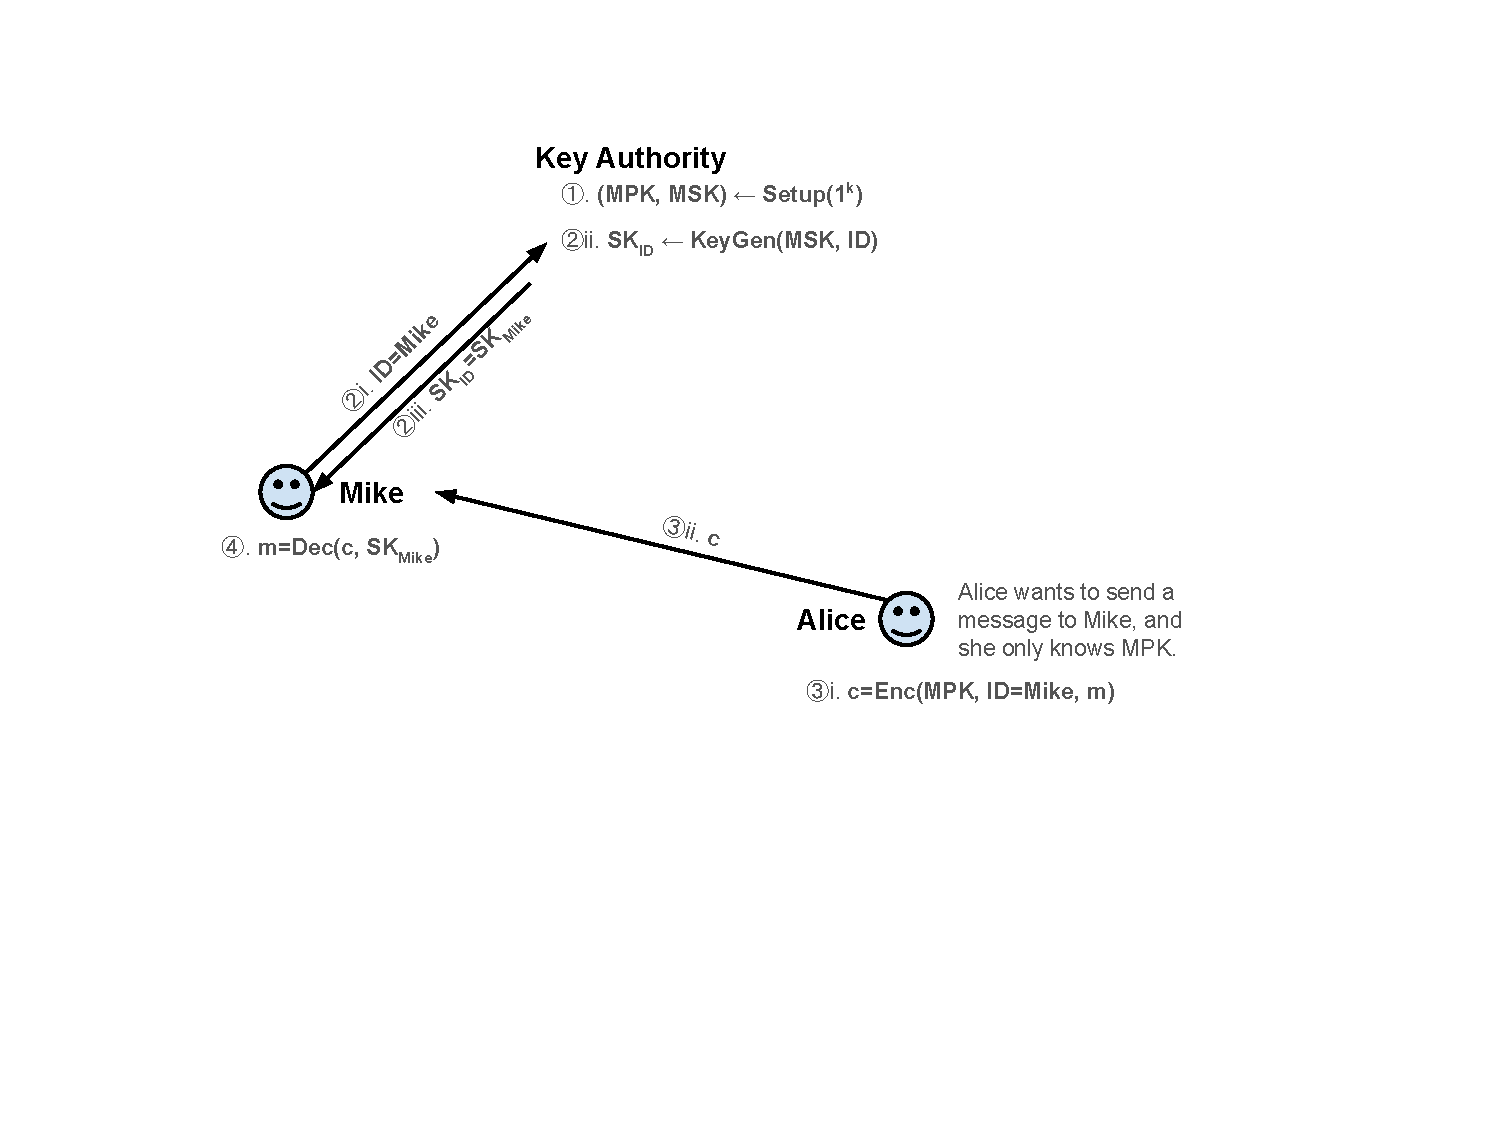
\includegraphics[width=0.7\textwidth]{Old Scribe Notes/fig3.pdf}
\caption{Identity-Based Encryption}
\end{figure}

Formally, we have

$$Pr\begin{bmatrix}
       (MPK, MSK) \gets Setup(1^k), \\[0.3em]
       SK_{ID} \gets KeyGen(MSK, ID), \\[0.3em]
       c \gets Enc(MPK, ID, m), \\[0.3em]
       m \gets Dec(SK_{ID}, c)
     \end{bmatrix}
      =1$$

\subsection{Security Descriptions}

We have different security descriptions for IBE, as discussed in this section.

\subsection{CCA1}
\begin{tabular}{ r c l }
  \textbf{Challenger} & & \textbf{Adversary} \\
  $(MPK, MSK) \gets Setup(1^k)$ & $\xrightarrow{MPK}$ &  \\
   & $\xleftarrow{ID_1}$ & \\
  $SK_{ID_1} \gets KeyGen(MSK, ID_1)$ & $\xrightarrow{SK_{ID_1}}$ & \\
  $\vdots$ & $\vdots$ & $\vdots$ \\
   & $\xleftarrow{ID_i}$ & \\
  $SK_{ID_i} \gets KeyGen(MSK, ID_i)$ & $\xrightarrow{SK_{ID_i}}$ & \\
   & $\xleftarrow{ID^*, m_0, m_1}$ & $\forall i \in [q], ID^* \neq ID_i$\\
  $b \overset{\$}{\gets} \{0, 1\}$, $c^* = Enc(MPK, ID^*, m_b)$ & $\xrightarrow{c^*}$ & \\
  Output $1$ if $b' = b$, otherwise $0$ & $\xleftarrow{b'}$ & \\
\end{tabular}

\subsection{CCA2}
In CCA2, we allow adversary to send further queries after getting $c^*$.

\begin{tabular}{ r c l }
  \textbf{Challenger} & & \textbf{Adversary} \\
  $(MPK, MSK) \gets Setup(1^k)$ & $\xrightarrow{MPK}$ &  \\
   & $\xleftarrow{ID_1}$ & \\
  $SK_{ID_1} \gets KeyGen(MSK, ID_1)$ & $\xrightarrow{SK_{ID_1}}$ & \\
   & $\vdots$ & \\
   & $\xleftarrow{ID_i}$ & \\
  $SK_{ID_q} \gets KeyGen(MSK, ID_q)$ & $\xrightarrow{SK_{ID_q}}$ & \\
   & $\xleftarrow{ID^*, m_0, m_1}$ & $\forall i \in [q'], ID^* \neq ID_i$\\
  $b \overset{\$}{\gets} \{0, 1\}$, $c^* = Enc(MPK, ID^*, m_b)$ & $\xrightarrow{c^*}$ & \\
   & $\xleftarrow{ID_{q+1}}$ & \\
  $SK_{ID_{q+1}} \gets KeyGen(MSK, ID_{q+1})$ & $\xrightarrow{SK_{ID_{q+1}}}$ & \\
  $\vdots$ & $\vdots$ & $\vdots$ \\
   & $\xleftarrow{ID_{q'}}$ & \\
  $SK_{ID_{q'}} \gets KeyGen(MSK, ID_{q'})$ & $\xrightarrow{SK_{ID_{q'}}}$ & \\
  Output $1$ if $b' = b$, otherwise $0$ & $\xleftarrow{b'}$ & \\
\end{tabular}

\subsection{Selective Security}
In selective security, the adversary sends $ID^*$ before everything.

\begin{tabular}{ r c l }
  \textbf{Challenger} & & \textbf{Adversary} \\
   & $\xleftarrow{ID^*}$ & $\forall i \in [q], ID^* \neq ID_i$\\
  $(MPK, MSK) \gets Setup(1^k)$ & $\xrightarrow{MPK}$ &  \\
   & $\xleftarrow{ID_1}$ & \\
  $SK_{ID_1} \gets KeyGen(MSK, ID_1)$ & $\xrightarrow{SK_{ID_1}}$ & \\
  $\vdots$ & $\vdots$ & $\vdots$ \\
   & $\xleftarrow{ID_q}$ & \\
  $SK_{ID_q} \gets KeyGen(MSK, ID_q)$ & $\xrightarrow{SK_{ID_q}}$ & \\
   & $\xleftarrow{m_0, m_1}$ & \\
  $b \overset{\$}{\gets} \{0, 1\}$, $c^* = Enc(MPK, ID^*, m_b)$ & $\xrightarrow{c^*}$ & \\
  Output $1$ if $b' = b$, otherwise $0$ & $\xleftarrow{b'}$ & \\
\end{tabular}


\subsection{Discussion 1}
How does Bilinear Maps apply to IBE?

Given Bilinear Maps: $(G, P, G_T, g, e)$, we have

\begin{enumerate}
\item $(G, P, G_T, g, e) \gets Setup(1^k)$
\item $s \gets Z^*_p$, and $H_1: \{0, 1\}^* \to G $, $H_2: G_T \to \{0, 1\}^n$
\item $MPK = (G, g^s, H_1, H_2)$, and $MSK = (s)$
\end{enumerate}

Let's look at how we construct each function in IBE.

\paragraph{$KeyGen(s, ID)$:}~\\
\begin{enumerate}
\item Output $SK_{ID} = (H_1(ID))^s$
\end{enumerate}

\paragraph{$Enc(MPK, ID, m)$:}~\\
\begin{enumerate}
\item $r \gets Z^*_p$
\item $c_1 = g^r$
\item $c_2 = m \oplus H_2(e(A, H_1(ID)^r))$, where $A = g^s$
\item Output $(c_1, c_2)$
\end{enumerate}

\paragraph{$Dec(SK_{ID}, (c_1, c_2))$:}~\\
\begin{enumerate}
\item Get $e(A, H_1(ID)^r) = e(H_1(ID)^s, c_1) = e(SK_{ID}, c_1)$
\item Get $m = c_2 \oplus H_2(e(A, H_1(ID))^r)$
\end{enumerate}

\proof
To prove this, we use a hybrid argument. Assume we have two oracles with exact random functions, denoted as $O_{H_1}$ and $O_{H_2}$.
One can request a random string from them with a query ID. The random strings are denoted as $H_1(ID)$ and $H_2(ID)$, respectively. These two oracles keep track of query IDs and corresponding responses. If a query ID was seen before, they return the exact same response corresponding to it. If not, they generate a random string, correspond the string to the ID, and return the string.

We first define $\mathcal{H}_0$, in which $H_1(ID)$ and $H_2(ID)$ are generated by the oracles. We use the construction described above.


\begin{tabular}{ r c l }
  \textbf{Challenger} & & \textbf{Adversary} \\
   & $\xleftarrow{\mathcal{G}, ID^*}$ & $\forall i \in [q], ID^* \neq ID_i$\\
   & $\xleftarrow{g^s}$ & \\
   & $\xleftarrow{O_{H_1}}$ & \\
   & $\xleftarrow{O_{H_2}}$ & \\
   & $\xleftarrow{ID_1}$ & \\
  $SK_{ID_1} \gets KeyGen(s, ID_1)$ & $\xrightarrow{SK_{ID_1}}$ & \\
  $\vdots$ & $\vdots$ & $\vdots$ \\
   & $\xleftarrow{ID_q}$ & \\
  $SK_{ID_q} \gets KeyGen(s, ID_q)$ & $\xrightarrow{SK_{ID_q}}$ & \\
   & $\xleftarrow{m_0, m_1}$ & \\
  $b \overset{\$}{\gets} \{0, 1\}$, $c^* = Enc(MPK, ID^*, m_b)$ & $\xrightarrow{c^*}$ & \\
  Output $1$ if $b' = b$, otherwise $0$ & $\xleftarrow{b'}$ & \\
\end{tabular}


Then we discard oracle's $H_1$, and use $H_1(ID) = g^{\alpha_{ID}}$, where $\alpha_{ID} \gets Z^*_p$. We denote this as $\mathcal{H}_1$.


Then we change $SK_{ID}$ to $SK_{ID} = (H_1(ID))^s = (g^{\alpha_{ID}})^s$. We denote this as $\mathcal{H}_2$.


We have Bilinear Decision Diffie-Hellman (DDH). If $\mathcal{H}_2$ breaks DDH, then $\mathcal{H}_0$ can as well.

In DDH, we have $(g^a, g^b, g^c, e(g, g)^{abc}) \stackrel{c}{\simeq} (g^a, g^b, g^c, e(g, g)^r)$.
We denote $A = g^a$, $B = g^b$, $C = g^c$. And in $\mathcal{H}_2$, we have $A = g^s$, $B = H_1(ID^*)$, $C = c_1 = g^r$.
And in $c_2 = m \oplus H_2(e(g^s, H_1(ID^*))^r)$, we have $T = H_2(e(g^s, H_1(ID^*))^r) = e(g, g)^{abc}$.

$\qed$



\section{Fully Homomorphic Encryption}
So far, we've seen private and public key encryption and different security properties (CPA, CCA). We've also seen some advanced encrpytion schemes like Identity-Based Encryption (IBE) that allow us to encrypt to an identity rather than a public key. 

Consider an example where Alice has a complex tax return to fill out and decides to use a tax return preparation service. The current pipeline is as follows:
\begin{enumerate}
    \item Alice sends her tax forms (W2, 1099, etc) to the service.
    \item The service prepares the tax return and sends it back to Alice.
    \item Alice sends the tax return to the IRS.
\end{enumerate}
However, in this process, the service has access to all of Alice's tax information, which is a privacy concern. 

Consider an alternate scenario where Alice encrypts her tax forms before sending them to the service. It would be ideal if the service could still prepare the tax return without decrypting the forms by performing operations on the encrypted data. In this case, the service learns nothing about Alice's tax information but is still able to prepare the tax return. This is the idea behind Fully Homomorphic Encryption (FHE). FHE was first presented in [Gentry09]~\cite{STOC:Gentry09} and has since been improved upon. We will present the construction from [GSW13]~\cite{C:GenSahWat13}.

FHE can be defined in either private or public key settings. The below construction is defined in the private key setting for message space $\mathbb{Z}_2$.

\begin{definition}[Fully Homomorphic Encryption (FHE)]
    A FHE scheme for message space $\mathbb{Z}_2$ and circuit class $\mathcal{C}$ is a tuple of algorithms $(\mathsf{Gen}, \mathsf{Enc}, \mathsf{Dec}, \mathsf{Eval})$ such that:
    \begin{itemize}
        \item $\mathsf{Gen}(1^\lambda) \rightarrow (\ek, \sk)$: The key generation algorithm takes a security parameter $\lambda$ and outputs a secret key $\sk$ and evaluation key $\ek$.
        \item $\mathsf{Enc}(\sk, m) \rightarrow c$: The encryption algorithm takes a public key $\sk$ and message $m$ and outputs a ciphertext $c$.
        \item $\mathsf{Dec}(\sk, c) \rightarrow m$: The decryption algorithm takes a secret key $\sk$ and ciphertext $c$ and outputs a message $m$.
        \item $\mathsf{Eval}(\ek, F, c_1, \ldots, c_l) \rightarrow c$: The evaluation algorithm takes an evaluation key $\ek$, a circuit $F \in \mathcal{C}$, and $l$ ciphertexts $c_1, \ldots, c_l$ and outputs a ciphertext $\tilde{c}$.
    \end{itemize}
\end{definition}

A FHE scheme satisfies the following properties:
\begin{itemize}
    \item \textbf{Correctness}: $\forall n \in \mathbb{N},\, \forall F \in \mathcal{C},\, \forall (\mu_1, \mu_2, \dots, \mu_l) \in \mathbb{Z}_2^l$,
    \begin{align*}
        \Pr[\mathsf{Dec}(\sk, \mathsf{Eval}(\ek, F, \mathsf{Enc}(\sk, \mu_1), \dots, \mathsf{Enc}(\sk, \mu_l))) &= F(\mu_1, \mu_2, \dots, \mu_l)] \\
        &= 1 - \text{negl}(\lambda)
    \end{align*}

    \item \textbf{Security}: The following two distributions are computationally indistinguishable:
    \begin{align*}
        \{(\ek, \mathsf{ct}_0): \mathsf{ct}_0 \gets \mathsf{Enc}(\sk, 0), (\ek, \sk) \gets \mathsf{Gen}(1^\lambda)\} \\
        \{(\ek, \mathsf{ct}_1): \mathsf{ct}_1 \gets \mathsf{Enc}(\sk, 1), (\ek, \sk) \gets \mathsf{Gen}(1^\lambda)\}
    \end{align*}

    \item \textbf{Compactness}: The size of the ciphertext $\mathsf{Eval}(\ek, F, c_1, \ldots, c_l)$ is equal to a fresh encryption of the output of the circuit $F$ on the plaintexts $\mu_1, \ldots, \mu_l$:
    \begin{align*}
        \forall i,\, c_i &= \mathsf{Enc}(\sk, \mu_i) \\
        \lvert \mathsf{Eval}(\ek, F, c_1, \ldots, c_l) \rvert &= \lvert \mathsf{Enc}(\sk, F(\mu_1, \ldots, \mu_l)) \rvert
    \end{align*}
\end{itemize}

The construction of FHE is based on the Learning With Errors (LWE) problem. The high-level construction is done in two steps:
\begin{enumerate}
    \item \textbf{Leveled FHE}: We first construct a leveled FHE scheme that can evaluate arbitrary circuits of bounded depth.
    \item \textbf{Bootstrapping}: We then use the leveled FHE scheme to construct a fully homomorphic encryption scheme.
\end{enumerate}

\subsection{Leveled FHE}
To present some intuition for how we get homomorphic properties, consider the following construction. Let $C \in \mathbb{Z}_q^{l \times l}$ be a matrix and $v \in \mathbb{Z}_q^l$ be an eigenvector of this matrix. The eigenvalue is chosen as the message being encrypted. \\
Given this, we can easily perform operations on ciphertexts that correspond to operations on the underlying plaintexts.
\begin{itemize}
    \item \textbf{Addition}: Given two ciphertexts $C_1$ and $C_2$, we have $(C_1 + C_2) v = C_1 v + C_2 v = (m_1 + m_2) v$.
    \item \textbf{Multiplication}: Given two ciphertexts $C_1$ and $C_2$, we have $(C_1 \cdot C_2) v = C_1 (C_2 v) = C_1 (m_2 v) = m_1 m_2 v$.
\end{itemize}
Note that this is not a secure construction as presented, since with enough samples we can solve a linear system to obtain the secret key. However, this gives us some intuition for how we can perform operations on encrypted data. To make this construction secure, we need to add noise to the ciphertexts (which is where LWE comes in). \\
However, a naive way of doing this does not work; suppose we have that $Cv = m v + e$ where $e$ is the (small) noise term. Then, even a single multiplication gives us $C_1 C_2 v = m_1 m_2 v + C_1 e_2$, where the noise term is no longer guaranteed to be small since $C$ has no such guarantees.

The construction of the leveled FHE scheme is as follows. We use the LWE problem with parameters $(n, m, q, \chi)$ where $n$ is the dimension of the secret key, $m$ is the dimension of the public key, $q$ is the modulus, and $\chi$ is the noise distribution. The scheme is defined for message space $\mathbb{Z}_2$. Additionally, set $l = (n+1) \log q$.
\begin{itemize}
    \item $\mathsf{Gen}(1^\lambda) \rightarrow (\ek, \sk)$: Sample $s' \gets \mathbb{Z}_q^{n}$ and set $s =  
    \begin{bmatrix}
        -s' \\
        1
    \end{bmatrix} \in \mathbb{Z}_q^{n+1}$. 

    \item $\mathsf{Enc}(\sk \in \mathbb{Z}_q^{n+1}, m \in \mathbb{Z}_2) \rightarrow C \in \mathbb{Z}_q^{l \times (n+1)}$: Sample $A \gets \mathbb{Z}_q^{l \times n}$ and $e \gets \chi^{l}$. Define $B = A \| As' + e$ and $C = B + m \cdot G$ for a fixed gadget~\cite{EC:MicPei12} matrix $G \in \mathbb{Z}_q^{l \times (n+1)}$.
    
    \begin{itemize}
        \item Note that by choice of $B$, we have that $Bs = A(-s') + A(s') + e = e$ is an encryption of zero (with noise). Similarly, $Cs = Bs + msG = e + msG$. 
        \item $G$ is a block matrix containing $(n+1)$ block column vectors of size $\log q$ each. Each vector is $g = (1, 2, 4, \ldots, 2^{\log q - 1})$. Concisely, we can define $G = I_{n+1} \otimes g$ where $\otimes$ is the Kronecker product.
        \item We also define a $\mathsf{Flatten}$ operation on the ciphertext that converts $C \in \mathbb{Z}_q^{l \times (n+1)}$ to $\tilde{C} \in \mathbb{Z}_q^{l \times l}$ by bit decomposing each element of $C$ and replacing the element with its bit vector. \\
        This ensures that each element of this matrix is a bit. Looking ahead, this allows us to multiply ciphertexts without too much noise growth.
    \end{itemize}
    
\end{itemize}
\input{lec17-F24}
\chapter{Proving Computation Integrity}

\section{Commitment Schemes}
\section{Zero-Knowledge Proofs}
Traditional Euclidean style proofs allow us to prove veracity of statements to others. However, such proof systems have two shortcomings: (1) the running time of the verifier needs to grow with the length of the proof, and (2) the proof itself needs to be disclosed to the verifier. In this chapter, we will provide methods enabling provers to prove veracity of statements of their choice to verifiers while avoiding the aforementioned limitations. In realizing such methods we will allow the prover and verifier to be probabilistic and also allow them to interact with each other.\footnote{Formally, they can be modeled as interactive PPT Turing Machines.}

\section{Interactive Proofs}
\begin{definition} {\normalfont\textbf{(Interactive Proof System)}} For a language L we have an \textit{interactive proof system} if $\exists$ a pair of algorithms (or better, interacting machines) $(\mathcal{P},\mathcal{V})$, where $\mathcal{V}$ is polynomial in $|x|$, and both can flip coins, such that:
		\begin{itemize}
			\item Completeness: $\forall x\in L$
		$$\Pr_{\mathcal{P},\mathcal{V}} \left[Output_{\mathcal{V}}(\mathcal{P}(x) \leftrightarrow \mathcal{V}(x))=1\right]=1,$$
			\item Soundness: $\forall x\notin L$, $\forall \mathcal{P}^*$
		$$\Pr_{\mathcal{V}} \left[Output_{\mathcal{V}}(\mathcal{P}^*(x) \leftrightarrow \mathcal{V}(x))=1\right]<neg(|x|),$$
		\end{itemize} where $Output_{\mathcal{V}}(\mathcal{P}(x) \leftrightarrow \mathcal{V}(x))$ denotes the output of $\mathcal{V}$ in the interaction between $\mathcal{P}$ and $\mathcal{V}$ where both parties get $x$ as input.
		We stress that $\mathcal{P}$ and $\mathcal{P}^*$ can be computationally unbounded. 
  \end{definition}



\paragraph{Interactive Proof for Graph Non-Isomorphism (GNI).} We say that two graphs $G_0$ and $G_1$ are isomorphic, denoted $G_0 \cong G_1$, if $\exists$ an isomorphism $f: V(G_0) \rightarrow V(G_1)$ s.t. $(u,v)\in E(G_0)$ iff $(f(u),f(v))\in E(G_1)$, where $V(G)$ and $E(G)$ are the vertex and edge sets of some graph $G$. On the other hand, $G_0$ and $G_1$ are said to be non-isomorphic, $G_0 \ncong G_1$, if $\nexists$ any such $f$, and $GNI=\lbrace(G_0,G_1)|\  G_0\ncong G_1\rbrace$ be the language that consists of pairs of graphs that are not isomorphic. 

GNI is not believed to have short proofs so an interactive proof could offer a prover a mechanism to prove to a polynomially bounded verifier that two graphs are non-isomorphic. 


The intuition behind a protocol to accomplish the above task is simple. Consider a verifier that randomly rename the vertices of one of the graphs and give it to the prover. Can the prover given the relabeled graph figure out which graph did the verifier start with?  If $G_0$ and $G_1$ were not isomorphic  then an unbounded prover can figure this out. However, in case $G_0$ and $G_1$ {are} isomorphic then the distribution resulting form random relabelings of $G_0$ and $G_1$ are actually identical. Therefore, even an unbounded prover has no way of distinguishing which graph the verifier started with. So the prover has only a $\frac12$ probability of guessing which graph the verifier started with. Note that by repeating this process we can reduce the success probability of a cheating prover to negligible. More formally:

%		If they consistently answer correctly, however, it would be hard to remain skeptical against $G_0 \ncong G_1$ as they beat the odds to almost impossible limits.  And so this interaction can ``prove" very strongly to the verifier that $(G_0,G_1)\in$ GNI.  Consider the protocol we can define from this:

		\begin{center}
			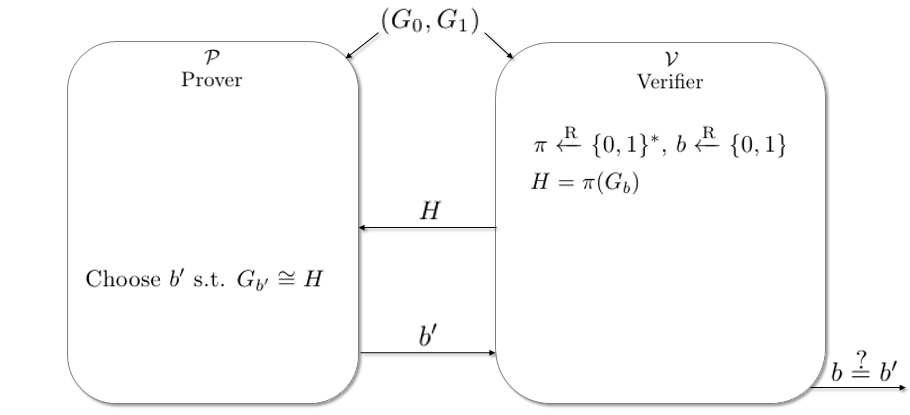
\includegraphics[scale=.51094]{Old Scribe Notes/GNI_IP_Protocol.png}
		\end{center}

		\begin{itemize}
			\item Completeness: If $(G_0,G_1)\in$ GNI, then the unbounded $\mathcal{P}$ can distinguish isomorphism of $G_0$ against those of $G_1$ and can always return the correct $b'$.  Thus, $\mathcal{V}$ will always output 1 for this case.
			\item Soundness: If $(G_0,G_1)\notin$ GNI, then it is equiprobable that $H$ is a random isomorphism of $G_0$ as it is $G_1$ and so $\mathcal{P}$'s guess for $b'$ can be correct only with a probability $\frac{1}{2}$.  Repeating this protocol $k$ times means the probability of guessing the correct $b'$ for all $k$ interactions is $\frac{1}{2^k}$.  And so the probability of $\mathcal{V}$ outputting 0 (e.g. rejecting $\mathcal{P}$'s proof at the first sign of falter) is $1-\frac{1}{2^k}$. 
		\end{itemize}

		%The interaction between prover and verifier captures the notion of a proof system for GNI, a problem previously not known to have an efficient method of proof.  By interacting, we can prove what seemed impossible to efficiently prove before!


\section{Zero Knowledge Proofs}


\begin{definition} {\normalfont\textbf{(NP-Verifier)}} A language L has an NP-verifier if $\exists$ a verifier $\mathcal{V}$ that is polynomial time in $|x|$ such that:
		\begin{itemize}
			\item Completeness: $\forall x\in L,\ \exists\ a\ proof\ \pi\ s.t.\ \mathcal{V}(x,\pi)=1$
			\item Soundness: $\forall x \notin L$ $\forall$ purported proof $\pi$ we have $\mathcal{V}(x,\pi)=0$
		\end{itemize}
  \end{definition}

		That is, the conventional idea of a proof is formalized in terms of what a computer can efficiently verify.  So a set of statements considered true (e.g. in a language $L$) is complete and sound if a proof can be written down that can be ``easily" and rigorously verified if and only if a statement is in the language.


\bigskip
\noindent\textbf{Efficient Provers.}
		Unfortunately (fortunately?), there aren't real-life instances of all-powerful provers that we know of.  And for cryptography we must make more reasonable assumptions about the provers.  In this case we will assume provers are also bounded to be \emph{efficient}.
		
		Previously, if a prover wanted to prove that two graphs, $G_0$ and $G_1$ were isomorphic, it would use its all-powerfulness to find the isomorphic mapping between the two graphs and give it to the verifier to complete the proof.  But now, being computationally bounded, the prover is in the same boat as the verifier and can find a proof no better than the verifier can.  In order for the prover to be able to prove something that the verifier cannot find out on their own, the prover must have some extra information.  If, for example, the prover simply knew the isomorphism between the graphs, this would be the sufficient extra information it needs to enact the proof.  That's a rather boring proof though.  We have interaction now!  Can't we do something fancier?
		
		What if the prover wanted to prove that two graphs were isomorphic but didn't want to fully reveal the isomorphism that they know.  If they're lying and don't know an isomorphism is their a way we can exploit them again?
		
		When $G_0$ and $G_1$ are isomorphic, the isomorphism between them would be a \textit{witness}, $w$, to that fact, that can be used in the proof.  Unfortunately, the prover is being stubborn and won't just tell us that isomorphism, $w:V(G_0)\rightarrow V(G_1)$, that they claim to have.  The prover is comfortable however giving us a ``scrambled" version, $\phi$, of $w$ as long as it doesn't leak any information about their precious $w$.  For example, the prover is willing to divulge $\phi = \pi \circ w$ where $\pi$ is a privately chosen random permutation of $|V|=|V(G_0)|=|V(G_1)|$ vertices.  Since $\pi$ renames vertices completely randomly, it scrambles what $w$ is doing entirely and $\phi$ is just a random permutation of $|V|$ elements.  At this point, we might be a little annoyed at the prover since we could have just created a random permutation on our own.  This might give us an idea on how to gain a little more information however, even though we gained none here:
		
		If we want to be convinced that $\phi$ really is of the form $\pi \circ w$, thus containing $w$ in its definition, and isn't just a completely random permuation, we can note that if it is of that form then $\phi(G_0)=\pi(w(G_0))=\pi(G_1)$ (since $w$ being an isomorphism implies that $w(G_0)=G_1$).  Note that we started with a mapping on input $G_0$ and ended with a mapping on input $G_1$.  With an isormphism, one could get from one graph to the other seamlessly; if the prover \textit{really} has the isomorphism it claims to have, then it should have no problem displaying this ability.  So, what if we force the prover to give us $H=\pi (G_1)$ just after randomly choosing its $\pi$ and then let it show us its ability to go from $G_1$ to $G_0$ with ease: give us a $\phi$ so that $\phi(G_0)=\pi(G_1)=H$.  The only way the prover can give a mapping that jumps from $G_0$ to $G_1$ in such a way is if they know an isomorphism; if the prover could find a $\phi$ efficiently but did \textit{not} know an isomorphism then they would have been able to see that $\pi^{-1}(\phi(G_0))=G_1$ and thus have $\pi^{-1}\circ\phi$ as an isomorphism from $G_0$ to $G_1$, which would contradict the assumed hardness of finding isomorphisms in the GI problem.  So by forcing the prover to give us $H$ as we've defined and to produce a $\phi$ so that $\phi(G_0)=H$, we've found a way to expose provers that don't really have an isomorphism and we can then be convinced that they really do know $w$ when they pass our test.  And the prover didn't directly tell us $w$, so they may be able to salvage some secrecy!
		
		But not everything is airtight about this interaction.  Why, for instance, would the prover be willing to provide $H=\pi(G_1)$ when they're trying to divulge as little information as possible?  The prover was comfortable giving us $\phi$ since we could have just simulated the process of getting a completely random permutation of vertices ourselves, but couldn't the additional information of $H$ reveal information about $w$?  At this point, the annoyed feeling may return as we realize that, $H=\pi(G_1)=\pi'(G_0)$, for some $\pi'$, is just a random isomorphic copy of $G_0$ \textit{and} $G_1$ as long as $G_0 \cong G_1$; we could have just chosen a random $\pi'$, set $H=\pi'(G_0)$, and let $\phi=\pi'$ and would have created our very own random isomorphic copy, $H$, of $G_1$ that satisfies our test condition $H=\phi(G_0)$ just like what we got from our interaction with the prover.  We couldn't have gained any new information from the prover because we could have run the whole test on our own!
		
		Well, something must be wrong; we couldn't have been convinced of something without gaining \textit{any} new information.  Indeed, the test has a hole in it: how can we force the prover to give us $H=\pi(G_1)$ like we asked?  If the prover is lying and it knows our test condition is to verify that $H=\phi(G_0)$, the prover might just cheat and give us $H=\pi(G_0)$ so it doesn't have to use knowledge of $w$ to switch from $G_1$ to $G_0$.  And, in fact, by doing this and sending $\phi=\pi$, the prover would fool us!
		
		To keep the prover on their toes, though, we can randomly switch whether or not we want $H$ to equal $\phi(G_0)$ or $\phi(G_1)$.  If, in our interaction, the prover must first provide their $H=\pi(G_1)$ before we let them know which we want, they then lock themselves into a commitment to either $G_0$ or $G_1$ depending on whether they're trying to cheat or not, respectively.  They only have a $50\%$ chance of committing to the same case we want on a given round and so, if they don't have $w$ to deftly switch between $G_0$ and $G_1$ to always answer correctly, they again have to be an extremely lucky guesser if they're trying to lie.
		
		Again, we've created an interactive scheme that can catch dishonest provers with probability 1-$\frac{1}{2^k}$ and where we always believe honest provers!
		
		\begin{center}
			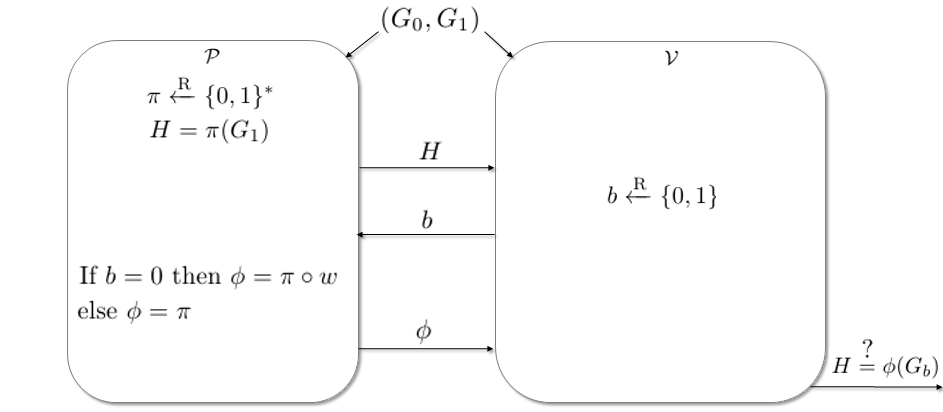
\includegraphics[scale=.51094]{Old Scribe Notes/GI_ZK_Protocol.png}
		\end{center}
		
		\begin{itemize}
			\item Completeness: If $(G_0,G_1)\in$ GI and $\mathcal{P}$ knows $w$, then whether $\mathcal{V}$ chooses $b=0$ or 1, $\mathcal{P}$ can always give the correct $\phi$ which, by definition, will always result in $H=\phi(G_b)$ and so $\mathcal{V}$ will always output 1.
			\item Soundness: If $(G_0,G_1)\notin$ GI, then $\mathcal{P}$ can only cheat, as discussed earlier, if the original $H$ it commits to ends up being $\pi(G_b)$ for the $b$ that is randomly chosen at the next step.  Since $b$ isn't even chosen yet, this can only happen by chance with probability $\frac{1}{2}$.  And so the probability $\mathcal{V}$ outputs 0 is $1-\frac{1}{2^k}$ for $k$ rounds.
		\end{itemize}
		
		And so, again, we've correctly captured the idea of a proof by having this interaction.  But there's a strange feeling that may be lingering around us...
		
		As a verifier, we've seen some things in interacting with the prover.  Surely, clever folks like ourselves must be able to glean \textit{some} information about $w$ after seeing enough to thoroughly convince us that the prover knows $w$.  We've first seen $H$, and we've also seen the random $b$ that we chose, along with $\phi$ at the end;  this is our whole view of information during the interaction.  But we're more bewildered than annoyed this time when we realize we could have always just chosen $b$ and $\phi$ randomly and set $H=\phi(G_b)$ on our own.  Again, everything checks out when $G_0 \cong G_1$ and we could have produced everything that we saw during the interaction before it even began.  That is, the distribution of the random variable triple ($H$, $b$, $\phi$) is identical whether it is what we saw from the prover during the interaction or it is yielded from the solitary process we just described.  We've just constructed a complete interactive proof system that entirely convinces us of the prover's knowledge of $w$, yet we could have simulated the whole experience on our own!  We couldn't have gain any knowledge about $w$ since we didn't see anything we couldn't have manufactured on own, yet we are entirely convinced that $(G_0,G_1)\in$ GI and that $\mathcal{P}$ knows $w$!  And so the prover has proven something to us yet has given us absolutely zero additional knowledge!
		
		This may feel very surprising or as if you've been swindled by a fast talker, and it very much should feel this way; it was certainly an amazing research discovery!  But this is true, and it can be made rigorous:
		
		We should first be sure what we want out of this new proof system.  We of course want it to be complete and sound so that we accept proofs iff they're true.  But we also want the verifier to gain zero knowledge from the interaction; that is, the verifier should have been able to simulate the whole experience on its own without the verifier.
		Finally, we would also like all witnesses to a true statement to each be sufficient to prove the veracity of that statement and so we let $R$ be the relation s.t. $x \in L$ iff $\exists$ a witness $w$ s.t. $(x,w)\in R$.  We can then gather all witness by defining $R(x)$ to be the set of all such witnesses.
		
		\begin{definition} {\normalfont\textbf{(Honest Verifier Zero Knowledge Proof [HVZK])}} For a language L we have a (perfect) \textit{HVZK proof system} w.r.t. witness relation $R$ if $\exists$ an interactive proof system, $(\mathcal{P},\mathcal{V})$ s.t. $\exists$ a PPT machine $\mathcal{S}$ (called the simulator) s.t. $\forall x \in L$, $\forall w\in R(x)$ the following distributions are identical:
		$$View_{\mathcal{V}}(\mathcal{P}(x,w) \leftrightarrow \mathcal{V}(x))$$
		$$\mathcal{S}(x)$$
		where $View_{\mathcal{V}}(\mathcal{P}(x,w) \leftrightarrow \mathcal{V}(x))$ is the random coins of $\mathcal{V}$ and all the messages $\mathcal{V}$ saw.
  \end{definition}

\begin{remark}
In the above definition, $View_{\mathcal{V}}(\mathcal{P}(x,w) \leftrightarrow \mathcal{V}(x))$ contains both the random coins of $\mathcal{V}$ and all the messages that $\mathcal{V}$ saw, because they together constitute the view of $\mathcal{V}$, and they are correlated. If the random coins of $\mathcal{V}$ are not included in the definition of $View_{\mathcal{V}}(\mathcal{P}(x,w) \leftrightarrow \mathcal{V}(x))$, then even if $\mathcal{S}$ can generate all messages that $\mathcal{V}$ saw with the same distribution as in the real execution, the verifier may still be able to distinguish the two views using its random coins.
\end{remark}
		
		There is an interesting progression of the requirements of a proof system: Completeness, Soundness, and the Zero Knowledge property.  Completeness first cares that a prover-verifier pair exist and can capture all true things as a team that works together; they both honestly obey the protocol trying prove true statements.  Soundness, however, assumes that the prover is a liar and cares about having a strong enough verifier that can stand up to any type of prover and not be misled.  Finally, Zero Knowledge assumes that the verifier is hoping to glean information from the proof to learn the prover's secrets and this requirement makes sure the prover is clever enough that it gives no information away in its proof.
		
		Unlike the soundness' requirment for a verifier to combat \textit{all} malicious provers, HVZK is only concerned with the verifier in the original prover-verifier pair that follows the set protocol.  Verifiers that stray from the protocol or cheat, however, are captured in the natural generalization to Zero Knowledge proofs.  
%		These are mostly discussed (including auxiliary inputs) in the next class, although the first definition is given below:
%		
%		{\definition {\normalfont\textbf{(Zero Knowledge Proof [ZK])}} For a language L we have a (perfect) \textit{ZK proof system} w.r.t. witness relation $R$ if $\exists$ an interactive proof system, $(\mathcal{P},\mathcal{V})$ s.t. $\exists$ a PPT machine $\mathcal{S}$ (called the simulator) s.t. $\forall x \in L$, $\forall w\in R(x)$, $\forall \mathcal{V}^*$, the following distributions are identical:
%		$$View_{\mathcal{V}^*}(\mathcal{P}(x,w) \leftarrow \mathcal{V}^*(x))$$
%		$$\mathcal{S}^{\mathcal{V}^*}(x)$$
%		where $\mathcal{S}^{\mathcal{V}^*}(x)$ is the simulator with oracle access to $\mathcal{V}^*$.}


% !TEX root = collection.tex

\begin{definition}[Efficient Prover Zero-Knowledge Proof]
We say $(P, V)$ is an efficient prover zero-knowledge proof system for a language $L$ and relation $R_L$ if \begin{enumerate}

\item The prover $P$ runs in polynomial time.

\item The protocol is \emph{complete}. That is, for every $x \in L$ there exists a witness $w \in R_L (x)$ such that $$\Pr [P(x,w) \leftrightarrow V(x) \ \emph{accepts}] = 1.$$

\item The protocol is \emph{sound} against unbounded provers. That is, for $\forall x \notin L$, we have $$\Pr [P^*(x,w) \leftrightarrow V(x) \ \emph{rejects}] \geq 1/2$$ for any prover $P^*$ of arbitrary computation power and any witness $w$.

\item There exists an expected polynomial time probabilistic machine $S$ (a simulator) such that for all PPT $V^*$, for all $x \in L, w \in R_L (x), z \in \{ 0, 1 \}^*$ we have $$\{ View_{V^*} (P(x,w) \leftrightarrow V^* (x,z)) \} \simeq_c \{ S^{V^*} (x,z) \} $$ \end{enumerate}

\end{definition}

The soundness probability can be amplified to be greater than any $1 - 1/2^k$, for arbitrary $k > 0$, by repeating the proof $k$ times. More precisely, we construct an efficient prover zero-knowledge proof system $(\tilde P, \tilde V)$ which repeats $(P,V)$ independently for $k$ times, and $\tilde V$ accepts if and only if $V$ accepts in all the executions.

It is easy to see that $\tilde P$ runs in polynomial time and that the protocol is complete.
Moreover, it has the following soundness guarantee:
for $\forall x \notin L$,
\begin{align*}
& \Pr \left[\tilde P^*(x,w) \leftrightarrow \tilde V(x) \ \text{rejects}\right]\\
= & 1- \Pr \left[\forall 1\leq i\leq k, P^*_i(x,w) \leftrightarrow V(x) \ \text{accepts}\right] \\
= & 1- \prod_{i=1}^k \Pr \left[P^*_i(x,w) \leftrightarrow V(x) \ \text{accepts}\right] \\
\geq& 1-\frac{1}{2^k}
\end{align*}
for any prover $\tilde P^*=(P^*_1, \cdots, P^*_k)$ of arbitrary computation power and any witness $w$.

Finally, it  is zero-knowledge, namely, there exists an expected PPT $\tilde S$ such that for all PPT $\tilde V^*$, and for all $x \in L, w \in R_L (x), z \in \{ 0, 1 \}^*$,
$$\left\{ View_{\tilde V^*} (\tilde P(x,w) \leftrightarrow \tilde V^* (x,z)) \right\} \simeq_c \left\{ \tilde S^{\tilde V^*} (x,z) \right\}.$$
The construction of $\tilde S$ is repeating $S$ for $k$ times. We prove by hybrid argument that the above two distributions are indistinguishable. $H_i$ is defined to be the output of repeating $S$ for the first $i$ executions with $\tilde V^*$ and repeating $P$ for the rest $k-i$ executions. Then $H_0$ is the left distribution and $H_k$ is the right one. Any attacher that can distinguish the above two distributions leads to an attacker that can distinguish $H_{i-1}$ and $H_{i}$ for some $1\leq i \leq k$, which violates the zero-knowledge property of the original proof system $(P,V)$.


\bigskip
The order of the quantifiers in item 4 matters.
If we quantify over $x$ and $w$ before quantifying over the simulator,
then we could hard-code  $x$ and $w$ into our simulator. That is, for all $x \in L, w \in R_L (x)$, there exists an expected polynomial time probabilistic machine $S_{x,w}$ such that for all PPT $V^*$ and $z \in \{ 0, 1 \}^*$,
$$\{ View_{V^*} (P(x,w) \leftrightarrow V^* (x,z)) \} \simeq_c \{ S_{x,w}^{V^*} (x,z) \} $$
Since we would like our simulator to be universal,  this is not acceptable.

If we quantify first over the verifier $V^*$ and then over simulators $S$, then this variant is considered as \emph{non-black-box zero-knowledge}. Our standard definition is considered as \emph{black-box zero-knowledge}. There  also exist variants that use statistical indistinguishability rather than computational indistinguishability.

The $z$ in item 4 is considered as \emph{auxiliary input}. The auxiliary input is crucial for the above argument of soundness amplification.

We will discuss the importance of requiring expected polynomial time in the next section.

\section{Graph Isomorphism}

Recall our protocol for graph isomorphism: the interaction is $P(x,w) \leftrightarrow V(x)$ where $x$ represents graphs $G_0 = (V, E_0)$ and $G_1 = (V, E_1)$ and $w$ represents a permutation $\pi$ on $V$ such that $\pi (G_0) = G_1$.

\begin{enumerate}
\item $P$ samples a random permutation $\sigma: V \to V$ and sends the graph $H = \sigma(G_1)$ to $V$.

\item $V$ samples a random bit $b$ and sends it to $P$.

\item If $b = 1$, then $P$ defines a permutation $\tau$ to be $\sigma$. If $b = 0$, then instead $\tau = \sigma \circ \pi$. $P$ then sends $\tau$ to $V$.

\item $V$ verifies that $\tau(G_b) = H$ and accepts if so.

\end{enumerate}

We will show that this is an efficient prover zero-knowledge proof system. It is clear that if $G_0$ and $G_1$ are isomorphic, then this protocol will succeed with probability 1.

For soundness, observe that if $G_0$ is not isomorphic to $G_1$, then the graph $H$ that $P$ sends to $V$ in step 1 of the protocol can be isomorphic to at most one of $G_0$ or $G_1$. Since $V$ samples a bit $b$ uniformly at random in step 2, then there is a probability of at most 1/2 that $P$ can produce a valid isomorphism in step 3.

For zero knowledge, consider the following simulator $S$ with input $G_0$ and $G_1$ (with vertex set $V$) and verifier $V^*$:

\begin{enumerate}
\item Guess a bit $b$ uniformly at random.

\item Sample a permutation $\pi: V \to V$ uniformly at random and send $\pi (G_b)$ to $V^*$.

\item Receive $b'$ form $V^*$.

\item If $b=b'$, then output $(\pi (G_b), b, \pi)$ and terminate. Otherwise, restart at step 1.

\end{enumerate}

Note that if $G_0 \simeq G_1$, then $\pi(G_b)$ is statistically independent of $b$ because $b$ and $\pi$ are sampled uniformly. Thus, with probability 1/2, $V^*$ will output $b$ so on average, two attempts will be needed before $S$ terminates. It follows that $S$ will terminate in \emph{expected} polynomial time.

Since $b$ is sampled uniformly at random, $\pi (G_b)$ is uniformly distributed with all graphs of the form $\sigma (G_1)$ where $\sigma$ is sampled uniformly at random from permutations on $V$. Thus, the output $\pi(G_b)$ in our simulator will be identically distributed with the output $H$ in our graph isomorphism protocol.

In step 3 of our graph isomorphism protocol, note that $\tau$ is distributed uniformly at random. This is because composing a uniformly random permutation with a fixed permutation will not change its distribution. Thus $\tau$ will be identically distributed with $\pi$ in our simulator. It follows that the transcripts outputted by our simulator will be identically distributed with the transcripts produced by the graph isomorphism protocol.

\section{Zero-Knowledge for NP}

An $n$-coloring of a graph $G = (A, E)$ is a function $c: A \to \{1, \ldots, n \}$ such that if $(i, j) \in E$, then $c(i) \neq c(j)$. So we want to paint each vertex of a graph a certain color so that the endpoints of any edge are colored differently.

In the graph 3-coloring problem (3COL), we are given a graph and asked if there exists a 3-coloring. In this section, we will provide a computational zero knowledge proof for 3COL. It is a fact that 3COL is NP-complete, so any problem in NP has a polynomial time reduction to 3COL. Thus, by giving a zero knowledge proof for 3COL, we will show that there are zero knowledge proofs for all of NP.

We will first give a high-level description of a zero-knowledge protocol for 3COL. Suppose a prover $P$ wants to convince a verifier $V$ that his graph $G$ is 3-colorable without revealing what the coloring $c$ actually is. If the three colors we use are red, green, and blue, then note that if we colored all the red vertices blue, all the green vertices red, and all the blue vertices green, we would still have a valid 3-coloring. In fact, if $\phi$ was any permutation on the color set of red, green, and blue, then $\phi \circ c$ would be a valid 3-coloring of $G$.

$P$ asks $V$ to leave the room and then samples a random permutation $\phi$ of the three colors. He colors the vertices of $G$ according to $\phi \circ c$, then covers all the vertices with cups. At this point, $P$ invites $V$ back into the room. $V$ is allowed to pick one edge and then uncover the two endpoints of the edge. If the colors on the two endpoints are the same, then $V$ rejects $P$'s claim that the graph is 3-colorable.

If the colors on the two endpoints are different, then $V$ leaves the room again, $P$ samples $\phi$ randomly, and the process repeats itself. Certainly if $G$ is actually 3-colorable, then $V$ will never reject the claim. If $G$ is not 3-colorable, then there will always be an edge with endpoints that are colored identically and $V$ will eventually uncover such an edge.

Note that $V$ does not gain any information on the coloring because it is masked by a (possibly) different random permutation every time $V$ uncovers an edge. Of course this protocol depends on $P$ not being able to quickly recolor the endpoints of an edge after removing the cups. This is why we need commitment schemes.

\subsection{Commitment Schemes}

We want to construct a protocol between a sender and a receiver where the sender sends a bit to the receiver, but the receiver will not know the value of this bit until the sender chooses to "open" the data that he sent. Of course, this protocol is no good unless the receiver can be sure that the sender was not able to change the value of his bit in between when the receiver first obtained the data and when the sender chose to open it.

\begin{definition}
A \emph{commitment scheme} is a PPT machine $C$ taking input $(b,r)$ that satisfies two properties: \begin{itemize}
\item (perfect binding) For all $r, s$, we have $C(0,r) \neq C(1,s)$.

\item (computational hiding) $\{ C(0, U_n) \} \simeq_c \{ C(1, U_n) \}$

\end{itemize}
\end{definition}

So for the sender to "open" the data, he just has to send his value of $r$ to the receiver. We say that $r$ is a \emph{decommitment} for $C(x,r)$. Why do we require perfect binding instead of just statistical binding? If there existed even a single pair $r, s$ where $C(0,r) = C(1,s)$, then the sender could cheat. If he wished to reveal a bit value of 0 then he could just offer $r$ and if he wished to reveal a bit value of 1 then he could just offer $s$.

We can use injective one-way functions to construct commitment schemes.

\begin{theorem}
If injective one-way functions exist, then so do commitment schemes.
\end{theorem}
\proof{We can let $f$ be an injective one-way function. Recall from Lecture 3 that $f' (x, r) := (f(x), r)$ will also be an injective one-way function with hard-core bit $B(x,r) := \langle x, r \rangle$. We claim that $C(b,x,r) := (f'(x,r), b \oplus B(x,r))$ is a commitment scheme.

If $(x,r)  \neq (y,s)$ then $C(0,x,r) \neq C(0,y,s)$ because $f'$ is injective. Since $C(0,x,r) = (f'(x,r), B(x,r)) \neq (f'(x,r), \overline{B(x,r)}) = C(1,x,r)$, then $C$ satisfies perfect binding.

Suppose $D$ can distinguish $C(0, U_n)$ from $C(1, U_n)$. Then we can distinguish $B(x,r)$ from $\overline{B(x,r)}$ given $f'(x,r)$ which contradicts the fact that $B(x,r)$ is a hard-core bit for $f'(x,r)$. Thus, $C$ has the computational hiding property.}
\qed

\medskip
We can extend the definition of commitment schemes to hold for messages longer than a single bit. These commitment schemes will work by taking our commitment schemes for bits and concatenating them together. For the extended definition, we require that for any two messages $m_0$ and $m_1$ of the same length, the ensembles $\{ C(m_0, U_n) \}$ and $\{ C(m_1, U_n) \}$ are computationally indistinguishable.

\subsection{3COL Protocol}

Below we describe the protocol $P(x,z) \leftrightarrow V(x)$, where $x$ describes a graph $G = (\{1, \ldots, n \}, E)$ and $z$ describes a 3-coloring $c$:

\begin{enumerate}
\item $P$ picks a random permutation $\pi : \{ 1, 2, 3 \} \to \{ 1, 2, 3 \}$ and defines the 3-coloring $\beta := \pi \circ c$ of $G$. Using a commitment scheme $C$ for the messages $\{ 1, 2, 3 \}$, $P$ defines $\alpha_i = C(\beta(i), U_n)$ for each $i \in V$. $P$ sends $\alpha_1, \alpha_2, \ldots, \alpha_n$ to $V$.

\item $V$ uniformly samples an edge $e = (i, j) \in E$ and sends it to $P$.

\item $P$ opens $\alpha_i$ and $\alpha_j$.

\item $V$ will accept only if it received valid decommitments for $\alpha_i$ and $\alpha_j$, and if $\beta(i)$ and $\beta(j)$ are distinct and valid colors.

\end{enumerate}

It is clear that this protocol is PPT. If $G$ is not 3-colorable, then there will be at least a $1/|E|$ probability that $V$ will reject $P$'s claim in step 4. Since $|E| \leq n^2$ we can repeat the protocol polynomially many times to increase the rejection probability to at least 1/2.

We will now show that this protocol is zero-knowledge. We describe a simulator $S$ below, given a verifier $V^*$: \begin{enumerate}
\item Sample an edge $e = (i, j) \in E$ uniformly at random.

\item Assign $c_i$ and $c_j$ to have distinct values from $\{ 1, 2, 3 \}$ and do so uniformly at random. Set $c_k := 1$ for all $k \neq i, j$.

\item Compute $n$ random keys $r_1, \ldots, r_n$ and set $\alpha_i = C(c_i, r_i)$ for all $i$.

\item Let $e' \in E$ be the response of $V^*$ upon receiving $\alpha_1, \ldots, \alpha_n$.

\item If $e' \neq e$, then terminate and go back to step 1. Otherwise, proceed. If $S$ returns to step 1 more than $2n |E|$ times, then output $\sf{fail}$ and halt the program.

\item Print $\alpha_1, \ldots, \alpha_n, e$, send $r_i$ and $r_j$ to $V^*$ and then print whatever $V^*$ responds with.
\end{enumerate}

By construction, $S$ will run in polynomial time. However, sometimes it may output a $\sf{fail}$ message. We will show that this occurs with negligible probability.

Suppose that for infinitely many graphs $G$, $V^*$ outputs $e' = e$ in step 4 with probability less than $1/2|E|$. If this is true, then it is possible for us to break the commitment scheme $C$ that we use in $S$. Consider a modified version of $S$ called $\tilde{S}$, where in step 2 we set $c_i = 1$ for all $i$. Note that in this case, $V^*$ cannot distinguish between any of the edges so the probability that it returns $e' = e$ is $1/|E|$.

If we gave $V^*$ a set of commitments $\alpha_k = C(1, r_k)$ for random keys $r_k$, then we would be in the setting of $\tilde{S}$. If we gave $V^*$ the commitments $\alpha_k$ but with two of the values set to $C(c, r)$ and $C(c', r')$ where $c, c'$ are distinct random values from $\{ 1, 2, 3 \}$ and $r, r'$ are random keys, then we are in the setting of $S$. This implies that it possible to distinguish between these two commitment settings with a probability of at least $1/2|E|$ which is non-negligible. It follows that $V^*$ outputs $e' = e$ with probability less than $1/2|E|$ for only finitely many graphs $G$.

Thus, the probability that $S$ outputs $\sf{fail}$ in the end is less than $(1 - 1/2|E|)^{2n|E|} < 1/e^n$ which is negligible.

Now we need to argue that the transcripts generated by $S$ are computationally indistinguishable from the transcripts generated by $P \leftrightarrow V^*$. Again, we consider a modified version of $S$, called $S'$, given a 3-coloring of its input $G$ as auxiliary input. In step 2 of the simulation, $S'$ will choose a random permutation of the colors in its valid 3-coloring for the values of $c_i$ rather than setting all but two values $c_i$ and $c_j$ equal to 1. Note that this is how our protocol between $P$ and $V$ behaves.

Observe that $P \leftrightarrow V^*$ is computationally indistinguishable from $S'$ because $S'$ outputs $\sf{fail}$ with negligible probability. Thus, it suffices to show that $S$ and $S'$ are computationally indistinguishable. Again, we will suppose otherwise and argue that as a result we can distinguish commitments.

We consider two messages $m_0$ and $m_1$ of the same length where $m_0$ consists of $n-2$ instances of the message $1$ and two committed colors $c_i$ and $c_j$ (for a random edge $(i, j) \in E$) and $m_1$ consists of a committed random 3-coloring of $G$ (with a random edge $(i, j) \in E$) chosen. Observe that by feeding the former message to $V^*$ we are in the setting of $S'$ and by feeding the latter message to $V^*$ we are in the setting of $S$. If we could distinguish those two settings, then we could distinguish the commitments for $m_0$ and $m_1$. This contradiction completes our argument that our 3-coloring protocol is zero-knowledge.
















%\newcommand{\st}{~\text{s.t.}~}
\newcommand{\rgets}{\overset{\$}{\gets}}
%\newcommand{\ind}{\overset{c}{\approx}}
\section{NIZK Proof Systems}
We now consider a different class of Zero-Knowledge proof systems, where no
interaction is required: The Prover simply sends one message to the Verifier,
and the Verifier either accepts or rejects. Clearly for this class to be
interesting, we must have some additional structure:
both the Prover and Verifier additionally have access to a common random public string
$\sigma$ (trusted to be random by both). For example, they could derive $\sigma$
by looking at sunspot patterns. 

\section{Definitions}

\begin{definition}[NIZK Proof System]
    A \emph{NIZK proof system} for input $x$ in language $L$, with witness $\omega$, is a set of
efficient (PPT) algorithms $(K, P, V)$ such that:
\begin{enumerate}
    \item Key Generation: $\sigma \gets K(1^k)$ generates the random public string.
    \item Prover: $\pi \gets P(\sigma, x, \omega)$ produces the proof.
    \item Verifier: $V(\sigma, x, \pi)$ outputs $\{0, 1\}$ to accept/reject the proof.
\end{enumerate}
Which satisfies the completeness, soundness, and zero-knowledge properties below.
\end{definition}
Note: We will assume throughout that $x$ is of polynomially-bounded length, i.e., we are
considering the language $L \cap \{0, 1\}^{P(k)}$.


\medskip
\noindent\textbf{Completeness.} $\forall x \in L, \forall \omega \in R_L(x)$:
    $$\Pr[\sigma \gets K(1^k), \pi \gets P(\sigma, x, \omega) : V(\sigma, x,
    \pi) = 1] = 1.$$

\medskip
\noindent\textbf{Non-Adaptive Soundness.} $\forall x \not\in L$:
    $$\Pr[\sigma \gets K(1^k): \exists~\pi \st V(\sigma, x, \pi)
    = 1] = \mathsf{negl}(k).$$
The above definition is ``non-adaptive", because it does not allow a cheating
prover to decide which statement to prove after seeing the randomness $\sigma$.
We may also consider the stronger notion of ``adaptive soundness", where the
prover is allowed to decide $x$ after seeing $\sigma$:

\medskip
\noindent\textbf{Adaptive Soundness.}
    $$\Pr[\sigma \gets K(1^k): \exists~ (x, \pi) \st  x \not\in L, V(\sigma, x, \pi)
    = 1] = \mathsf{negl}(k).$$
    
\medskip
\noindent\textbf{(Non-Adaptive) Zero-Knowledge.}
    The exists a PPT simulator $S$ such that $\forall x \in L, \omega \in
    R_L(x)$, the two distributions are computationally indistinguishable:

\begin{minipage}{0.5\textwidth}
    \begin{enumerate}[itemsep=-3pt]
        \item $\sigma \gets K(1^k)$
        \item $\pi \gets P(\sigma, x, \omega)$
        \item Output $(\sigma, \pi)$
    \end{enumerate}
\end{minipage}
\begin{minipage}{0.5\textwidth}
    \begin{enumerate}
        \item $(\sigma, \pi) \gets S(1^k, x)$
        \item Output $(\sigma, \pi)$
    \end{enumerate}
\end{minipage}

\medskip
That is, the simulator is allowed to generate the distribution of randomness
$\sigma$ together with $\pi$. Note that if we did not allow $S$ to produce
$\sigma$, this definition would be trivial (a verifier could convince himself by
running the simulator, instead of interacting with $P$). Allowing $S$ to
generate $\sigma$ still keeps the definition zero-knowledge (since a verifier sees both $(\sigma,
\pi)$ together), but puts $P$ and $S$ on unequal footing.

We could also consider the adaptive counterpart, where a cheating verifier can
choose $x$ after seeing $\sigma$:

\medskip
\noindent\textbf{(Adaptive) Zero-Knowledge.}
    The exists a PPT simulator split into two stages $S_1, S_2$ such that
    for all PPT attackers $\ma$,
    the two distributions are computationally indistinguishable:

\medskip
\begin{minipage}{0.5\textwidth}
    \begin{enumerate}[itemsep=0pt]
        \item $\sigma \gets K(1^k)$
        \item $(x, \omega) \gets \ma(\sigma)$, s.t. $(x, \omega) \in R_L$
        \item $\pi \gets P(\sigma, x, \omega)$
        \item Output $(\sigma, x, \pi)$
    \end{enumerate}
\end{minipage}
\begin{minipage}{0.5\textwidth}
    \begin{enumerate}[itemsep=0pt]
        \item $(\sigma, \tau) \gets S_1(1^k)$
        \item $(x, \omega) \gets \ma(\sigma)$
        \item $\pi \gets S_2(\sigma, x, \tau)$
        \item Output $(\sigma, x, \pi)$
    \end{enumerate}
\end{minipage}

\medskip
\noindent where $\tau$ should be thought of as local state stored by the simulator (passed
    between stages).

\bigskip
Now we show that adaptive soundness is not harder to achieve than non-adaptive soundness.
\begin{theorem}\label{thm:amplify-soundness}
    Given a NIZK $(K, P, V)$ that is \emph{non-adaptively sound}, we can
    construct a NIZK that is \emph{adaptively sound}.
\end{theorem}
\proof
For $x_0 \not\in L$, let us call a particular $\sigma$ ``bad for $x_0$" if 
there exists a false proof for $x_0$ using randomness $\sigma$:
$\exists~ \pi \st V(\sigma, x_0, \pi) = 1$.
By non-adaptive soundness of $(K, P, V)$, we have
$\Pr_\sigma[\sigma \text{ bad for } x_0] = \mathsf{negl}(k)$.

Now we construct a new NIZK $(K',P',V')$ by repeating $(K,P,V)$ polynomially-many times
(using fresh randomness, and $V'$ accepts if and only if $V$ accepts in each iteration).
We can ensure that $\mathsf{negl}(k) \leq 2^{-2P(k)}$.
Now by  union bound:
$$
\Pr[\sigma \gets K'(1^k): \exists~ (x, \pi) \st V'(\sigma, x, \pi) = 1] \leq
2^{P(k)}\cdot \Pr_\sigma[\sigma \text{ bad for } x_0] \leq 2^{-P(k)}.$$
So this new NIZK is adaptively-sound. \qed

\section{Trapdoor One-Way Permutation}

\begin{definition}[Trapdoor One-Way Permutation]
A trapdoor one-way permutation is a collection of one-way permutations $\{f_i : D_i \rightarrow D_i\}_{i \in I}$ where $D_i \subset \{0,1\}^{|i|}$ with
five properties.

\begin{enumerate}
\item $\exists$ PPT $G$ such that $G(1^k)$ outputs $(i,t_i)$ where $i \in I\cap \binset{k}$
\item It is easy to sample from $D_i$ given $i$ 
\item $f_i$ is easy to compute but hard to invert
\item  $f_i$ is a permutation
\item $\exists$ PPT $A$ such that $A(i, y, t_i)\in f_i^{-1}(y)$
\end{enumerate}
\end{definition}

When $f_i$ is a one-way trapdoor permutation, it is a one-way permutation with
the property that it is easy to compute $f_i^{-1}$ only if given access to trapdoor
information $t_i$. The function $G$ is PPT and computes this trapdoor information.
The function $A$ is PPT and inverts $f_i$ using this trapdoor information.

\subsection{RSA}

RSA is the only known example of a trapdoor one-way permutation.
It relies on the assumption that factoring numbers is hard,
but testing primality is easy. (It is known that testing primality can be done
deterministically in polynomial time. It is believed that factoring can not be done in
polynomial time, however this has not been proven. The best factoring algorithms
are sub-exponential though.)

\begin{definition}
RSA defines the functions $(G, F, A)$ as follows.
\begin{align*}
G(1^k) = ((N, e), d) \,\,\text{where} \,\,& N=pq, \,\, \text{for primes $p,q$},  \\
& \gcd(e,\phi(N))=1 \\
& d = e^{-1} \pmod{\phi(N)} \\
F_{N,e}(x) = x^e \pmod{N} & \\
A((N,e),y, d) = y^d \pmod{N} &
\end{align*}
\end{definition}

The function $G$ randomly selects the values of $(p, q, e)$ to satisfy the desired properties. We note that if  $e$ were not coprime to $\phi(N)$, then the function would
not be a permutation.

The function $\phi$ is Euler's Totient, and when $p,q$ are primes,
$\phi(pq) = (p-1)(q-1)$.
(That is, $\phi$ is the order of the multiplicative group $\mathbb{Z}_N$.)

The trapdoor piece of information is the multiplicative inverse of $e$ modulo the order of the
group. It is believed hard to compute this information given only the integer $N$.

It is easy to show correctness of this scheme:
\begin{align*}
A(i, F_i(x), t_i) &= (x^e)^d = x \pmod{N}
\end{align*}

We leave it as an exercise that RSA is semantically
secure with no additional assumptions.

\section{NIZK in the Hidden-Bit Model}
The hidden-bit model is a variant of the common-reference-string NIZK,
where the prover can selectively reveal only parts of the random string to the
verifier. (Imagine clouds obscuring the random string in the sky from the
verifier, and the prover can choose which clouds to clear.)

\newcommand{\setI}[1]{\{#1\}_{i \in I}}
\begin{definition}[NIZK in the Hidden-Bit Model]
    A NIZK in the hidden-bit model for statement $x$ (with witness $\omega$)
    is efficient algorithms $(K_H, P_H, V_H)$
    such that:
\begin{enumerate}
    \item $r \gets K_H(1^k)$ generates the hidden random string ($\ell$-bits).
    \item $(I, \phi) \gets P_H(r, x, \omega)$ generates the indices $I \subseteq
        [\ell]$ to reveal, and the proof $\phi$.
    \item $V_H(I, \setI{r_i}, x, \phi)$ accepts or rejects, given the indices $I$,
        the random string $r$ at indices $I$, statement $x$, and proof $\phi$.
\end{enumerate}
Which satisfies the completeness, soundness, and zero-knowledge properties as
previously defined.
\end{definition}


\begin{theorem}\label{thm:NIZK-amplify}
    Given a NIZK $(P_H, V_H)$ in the hidden-bit model, we can construct a NIZK
    $(P, V)$ in the normal model using trapdoor one-way permutations.
\end{theorem}
\begin{proof}
    Let the common-reference-string $\sigma$ in the normal model be of length $k\ell$ and  partition it
    into $\ell$ blocks of $k$-bits each: $\sigma = \sigma_1\hdots\sigma_\ell$.
    Let $\mathcal{F}$ be a family of $2^k$ trapdoor OWPs, and let $B(\cdot)$
    be the corresponding hard-core bit. We may assume the soundness error
    of $(P_H, V_H)$
    (that is, the probability of $r$ allowing a fake proof)
    is at most $2^{-2k}$, by the same repetition argument as in Theorem~\ref{thm:amplify-soundness}.
    The protocol for the normal $(P, V)$ is:

\medskip
\noindent \textbf{Prover $P(\sigma, x, \omega)$:}
\begin{enumerate}
    \item Sample trapdoor OWP: $(f, f^{-1}) \gets \mathcal{F}(1^k)$.
    \item Let $\alpha_i = f^{-1}(\sigma_i)$ for $\forall i \in [\ell]$.
    \item Compute hidden-bit $r_i = B(\alpha_i)$ for $\forall i \in [\ell]$. Let $r := r_1 \cdots r_\ell$.
    \item Run the HBM prover: $(I, \phi) \gets P_H(r, x, \omega)$.
    \item Send $(f, I, \setI{\alpha_i}, \phi)$ to verifier.
\end{enumerate}

\noindent \textbf{Verifier $V(\sigma, x, f, I, \setI{\alpha_i}, \phi)$:}
\begin{enumerate}
    \item Confirm $f \in \mathcal{F}$, and $f(\alpha_i) = \sigma_i ~\forall i \in I$.
    \item Compute the revealed bits $r_i = B(\alpha_i) ~\forall i \in I$.
    \item Output $V_H(I, \setI{r_i}, x, \phi)$.
\end{enumerate}

Intuitively, $\sigma_i$ hides $r_i$ because $\sigma_i \overset{f}{\gets} \alpha_i
\overset{B}{\to} r_i$, so by security of the hard-core bit, the verifier cannot
find $r_i = B(\alpha_i)$ from $\sigma_i = f(\alpha_i)$.

Notice that if the prover is honest, then $\alpha_i$ will be distributed
uniformly random as well (since $f^{-1}$ is a permutation), and $r_i$ will be
unbiased as well (since $B(\cdot)$ is a hard-core bit). So this reduces exactly
to the HBM distributions, and completeness of this protocol is clear (from completeness of
$(P_H, V_H)$).

For soundness: for a fixed $f = f_0$, the distribution of $r_i$ is
uniformly random, so by the soundness of $(P_H, V_H)$ we have
$$\Pr_\sigma[\text{$P^*$ can cheat using $f_0$}] \leq 2^{-2k}$$
However, a cheating $P^*$ may be able to cleverly pick $f$ to influence $r_i$,
allowing him to cheat. Since we know there are only $2^k$ possible choices of
$f$ (the verifier confirms $f$ is properly sampled), we can use the union bound
to prove soundness:
$$\Pr_\sigma[~\exists \text{ some $f \in \mathcal{F}$ s.t. $P^*$ can cheat}] \leq 2^{-k}.$$

Note that more serious problems can occur if $V$ does not confirm $f\in \mathcal{F}$. For example, if $f$ is not a permutation, then
$f^{-1}(\sigma_i)$ can be multi-valued, and the prover can choose to ``explain"
$\sigma_i$ using either $\alpha_i$ or $\alpha_i'$ -- which is a problem if
$B(\alpha_i) \neq B(\alpha_i')$.

To prove zero-knowledge, we construct a sequence of prover-hybrids.
Differences from the previous hybrid are in red:

%\newcommand{\htitle}[1]{#1\\
%\rule{0.2\textwidth}{0.4pt}}

\newcommand{\htitle}[1]{\vspace{0.3cm}$\overset{#1}{\underline{\hspace{5cm}}}$}
\newcommand{\diff}[1]{{\color{red} #1}}

\htitle{H_0 \text{ (normal model)}}
\begin{enumerate}
    \item $\sigma_1\hdots\sigma_\ell = \sigma \xleftarrow{\$} \{0,1\}^{k\ell}$
    \item $(f, f^{-1}) \gets \mathcal{F}$
    \item $\alpha_i = f^{-1}(\sigma_i) ~\forall i \in [\ell]$
    \item $r_i = B(\alpha_i) ~\forall i \in [\ell]$
    \item $(I, \phi) \gets P_H(r, x, \omega)$
    \item Output $(\sigma, f, I, \setI{\alpha_i}, \phi)$
\end{enumerate}

\htitle{H_1}
\begin{enumerate}
    \item $(f, f^{-1}) \gets \mathcal{F}$
    \item \diff{$\alpha_i \rgets \{0, 1\}^k ~\forall i \in [\ell]$}
    \item \diff{$\sigma_i = f(\alpha_i) ~\forall i \in [\ell]$}
    \item $r_i = B(\alpha_i) ~\forall i \in [\ell]$
    \item $(I, \phi) \gets P_H(r, x, \omega)$
    \item Output $(\sigma, f, I, \setI{\alpha_i}, \phi)$
\end{enumerate}
In $H_1$, we sample $\alpha_i$ uniformly at random and then generate $\sigma_i$ (instead of
sampling $\sigma_i$ and then generating $\alpha_i$). This induces an exactly identical distribution, since $f$
is a permutation.

\htitle{H_2}
\begin{enumerate}
    \item $(f, f^{-1}) \gets \mathcal{F}$
    \item \diff{$r_i \rgets \{0, 1\} ~\forall i \in [\ell]$}
    \item \diff{$\alpha_i \rgets B^{-1}(r_i) ~\forall i \in [\ell]$}
    \item $\sigma_i = f(\alpha_i) ~\forall i \in [\ell]$
    \item $(I, \phi) \gets P_H(r, x, \omega)$
    \item Output $(\sigma, f, I, \setI{\alpha_i}, \phi)$
\end{enumerate}
In $H_2$, we again switch the sampling order: first sample the (unbiased) bit
$r_i$, then sample $\alpha_i$ from the pre-image of $r_i$ (which can be done efficiently
by simply trying random $\alpha_i$'s until $B(\alpha_i) = r_i$).
This distribution is exactly identical to $H_1$.
(The sampling order can be thought of as factoring the joint distribution:
$\Pr(\alpha_i, r_i) = \Pr(r_i)\Pr(\alpha_i | r_i)$)

\htitle{H_3}
\begin{enumerate}
    \item $(f, f^{-1}) \gets \mathcal{F}$
    \item $r_i \rgets \{0, 1\} ~\forall i \in [\ell]$
    \item $\alpha_i \rgets B^{-1}(r_i) ~\forall i \in [\ell]$
    \item \diff{$\sigma_i = f(\alpha_i) ~\forall i \in I$}
    \item \diff{$\sigma_i \rgets \{0, 1\}^k ~\forall i \not\in I$}
    \item $(I, \phi) \gets P_H(r, x, \omega)$
    \item Output $(\sigma, f, I, \setI{\alpha_i}, \phi)$
\end{enumerate}
In $H_3$, we only generate $\sigma_i$ honestly for $i \in I$, and output random
$\sigma_i$ for $i \not\in I$.
To argue that this is computational
indistinguishable from $H_2$, first notice that for a fixed (known) bit $r$,
\begin{equation}
\label{eqn:bit-ind}
\{f(B^{-1}(r)\} \ind \{f(B^{-1}(\overline r)\}
\end{equation}
where the randomness is over sampling the pre-image $B^{-1}$.
Distinguishing the above distributions is by definition equivalent to guessing the
hard-core bit, so they are indistinguishable.
Given the above, we can further argue that
\begin{equation}
\label{eqn:rand-ind}
\{f(B^{-1}(r)\} \ind \mathcal{U}_k
\end{equation}
where $\mathcal{U}_k$ is uniform over $\{0, 1\}^k$. To see this, notice
that $\mathcal{U}_k$ can be equivalently generated by first sampling a random
bit $b$, then outputting $f(B^{-1}(b))$, since $f$ is a permutation.
Therefore, any distinguisher for \eqref{eqn:rand-ind} can also be used to distinguish
\eqref{eqn:bit-ind} with at least as much distinguishing-advantage (in fact,
twice as much).
Finally, \eqref{eqn:rand-ind} justifies swapping $\sigma_i = f(\alpha_i) =
f(B^{-1}(r_i))$ with random for $i \not\in I$ in hybrid $H_3$.





\htitle{H_4}
\begin{enumerate}
    \item $(f, f^{-1}) \gets \mathcal{F}$
    \item \diff{$(I, \setI{r_i}, \phi) \gets S_H(1^k, x)$}
    \item \diff{$\alpha_i \rgets B^{-1}(r_i) ~\forall i \in I$}
    \item $\sigma_i = f(\alpha_i) ~\forall i \in I$
    \item $\sigma_i \rgets \{0, 1\}^k ~\forall i \not\in I$
    \item Output $(\sigma, f, I, \setI{\alpha_i}, \phi)$
\end{enumerate}
Finally, $H_4$ simply swaps the hidden-bit prover $P_H$ for the hidden-bit simulator $S_H$,
which is indistinguishable by the zero-knowledge property of $(P_H, V_H)$.
So $(P, V)$ is a NIZK system in the normal model.
\qed

\end{proof}



\section{NIZK in the Hidden-Bit Model for  Graph Hamiltonian}

\begin{definition}
A Hamiltonian cycle in a graph is a cycle that visits each vertex exactly once. A Hamiltonian graph is a graph that contains a Hamiltonian cycle. More precisely, given a graph
$G=(V,E)$ with $|V|=n$, we say that $G$ is a Hamiltonian graph if there are
$x_1,\ldots,x_n\in V$ such that they are all distinct vertices, and $\forall i\in\{1,\ldots,n-1\} : (x_i,x_{i+1})\in E$,
$(x_n,x_1)\in E$.
\end{definition}


It is well known that the problem of determining if a graph is Hamiltonian is $NP$-complete.
Here we will construct a NIZK proof in the hidden-bit model (HBM) that is able to prove
that a graph is Hamiltonian.

First we define how graphs are represented as matrices.

\begin{definition}
A graph $G=(V,E)$ with $|V|=n$, can be represented as an $n\times n$ adjacency matrix $M_G$
of boolean values such that
$M_G[i,j]=\left\{
\begin{array}{l l}
1 & \text{if $(i,j)\in E$,} \\
0 & \text{otherwise.}
\end{array}
\right.$

A \emph{cycle matrix} is a matrix which corresponds to a graph that contains a Hamiltonian cycle and
contains no edges other than this cycle.

A \emph{permutation matrix} is a boolean matrix such that each row and each column has exactly one
entry equal to 1.
\end{definition}

\begin{figure}[ht]
	\centering
		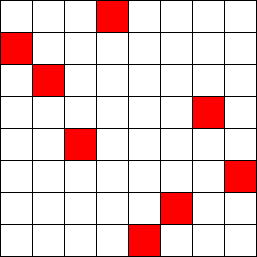
\includegraphics[height=4cm]{Old Scribe Notes/cycle.png}
	\caption{Cycle matrix.}
	\label{fig:cycle}
\end{figure}

\begin{figure}[ht]
	\centering
		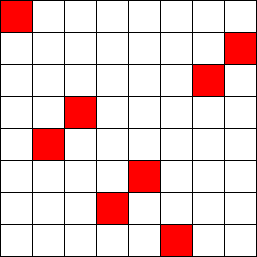
\includegraphics[height=4cm]{Old Scribe Notes/permutation.png}
	\caption{Permutation matrix.}
	\label{fig:permutation}
\end{figure}

Every cycle matrix is a permutation matrix, but the converse is not true.
For each size $n$, there are $n!$ different permutation matrices but
only $(n-1)!$ cycle matrices.

In Figure~\ref{fig:cycle}, one can see the cycle matrix as a cycle $(1,4,7,6,8,5,3,2)$
on the set $\{1,2,3,4,5,6,7,8\}$. In Figure~\ref{fig:permutation}, it is possible to
interpret the matrix as a permutation $(1)(2,8,6,5)(3,7,4)$ on the same set.

\begin{theorem}
There is a non-interactive zero-knowledge (NIZK) proof in the
hidden-bit model (HBM) for the problem of proving that a graph is Hamiltonian.
\end{theorem}
\proof
In the hidden-bit model (HBM), there is a random string $r$ with $\ell$ bits that the prover
can read. The prover should be able to produce a proof $\phi$ and choose a set
$I\subseteq\{1,2,\ldots,\ell\}$ such that the proof and the bits of the string corresponding to
the set $I$ will be revealed to the verifier.
\begin{table}[ht]
\centering
\begin{tabular}{r c l}
%\mright{P}{\phi,I,\{r_i \mid i\in I\}}{V}
\end{tabular}
\end{table}


Let the graph be $G=(V,E)$ with $|V|=n$.
The objective is to convince the verifier that the assertion is correct (the graph $G$
is Hamiltonian).

Suppose that the random string $r$ comes from a distribution
such that this string represents the entries from an $n\times n$ cycle matrix $M_c$.
Then a proof can be produced as follows.

Since the prover $P$ knows the Hamiltonian cycle $x_1,\ldots,x_n$ in $G$, he can find a
function $\phi:V\rightarrow \{1,2,\ldots,n\}$ that puts the Hamiltonian cycle exactly
over the cycle of $M_c$. More precisely, for this function we have
$M_c[\phi(x_i),\phi(x_{i+1})]=1$ for each edge $(x_i,x_{i+1})$ in the Hamiltonian cycle of G
(we view indices modulo $n$).
This means that all the edges of $M_c$ will be covered by edges of $G$. Conversely, all the
non-edges of $G$ must be taken to non-edges of $M_c$.

So the strategy for the prover is to reveal the mapping $\phi$ and also reveal entries of $M_c$ corresponding to $\phi(e)$ where $e \notin E$. More precisely, for the set
$I=\{(\phi(u),\phi(v)) \mid (u,v)\notin E\}$, $P$ reveals
$M_c[\phi(u),\phi(v)]=0$,
which proves that $(\phi(u),\phi(v))$ is a non-edge of $M_c$.

\begin{figure}[ht]
	\centering
		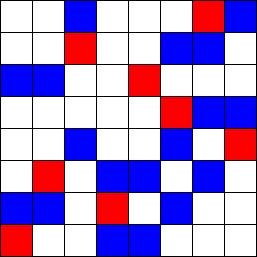
\includegraphics[height=4cm]{Old Scribe Notes/red_blue.png}
	\caption{Graph matrix that includes a Hamiltonian cycle. Edges are blue/red and the
                 cycle is red. White cells are non-edges.}
	\label{fig:red_blue}
\end{figure}

A visual example is shown in Figure~\ref{fig:red_blue}. The cycle graph $M_c$ given by the
random string corresponds to the red cells. These cells have value 1 in the matrix $M_c$ and
all other cells have value 0. The prover $P$ provides a bijection $\phi$ that
maps the edges of $G$ to this matrix in such a way that all red cells are covered and
some others may also be covered (blue cells). The important property guaranteed is that
all the non-edges of $G$ are mapped to cells that have a value 0 in the matrix (white cells).

This proof satisfies the three properties required for a zero knowledge proof.

\textit{Completeness:} if $P$ and $V$ are both honest, then $P$ will be able to convince
$V$ that the statement is true. That's because $P$ knows the Hamiltonian cycle of $G$,
hence he is always able to produce the mapping $\phi$.

\textit{Soundness:} if $P$ is lying and trying to prove a false statement, then he will
get caught with probability 1. If $P$ does not know any Hamiltonian cycle in $G$, then
any function $\phi$ he chooses will not cover all the edges in $M_c$. Hence there will
be an entry in the matrix $M_c$ which is one and will be revealed as a non-edge of $G$.

\textit{Zero Knowledge:} $V$ cannot get any information besides the fact that $P$
knows a Hamiltonian cycle in $G$. A simulator $S$ for this proof can be simply a machine
that generates a random permutation $\phi:V\rightarrow \{1,2,\ldots,n\}$ and reveals zeros
for all the non-edges of $\phi(G)$.

\vspace{5mm}

In this proof we assumed that the random string $r$ comes from a very specific distribution
that corresponds to cycle matrices.
Now we need to show that the general problem (where $r$ comes from a
random uniform distribution of $\ell$ bits) can be reduced into this previous scenario.

We proceed as follows.
Let the length of the random string be
$\ell=\left\lceil 3\cdot \log_2 n\right\rceil \cdot n^4$.
We view the random string $r$ as $n^4$ blocks of $\left\lceil 3\cdot \log_2 n\right\rceil$
bits and we generate a random string $r'$ of length $n^4$ such that each bit in $r'$
is 1 if and only if all the bits in the corresponding block of $r$ are equal to 1.
This way, the probability that the $i$-th bit of $r'$ equals 1 is $\Pr[r'_i=1]\approx\frac{1}{n^3}$ for every $i$.

Then we create an $n^2\times n^2$ matrix $M$ whose entries are given by the bits of $r'$.
Let $x$ be the number of one entries in the matrix $M$.
The expected value for $x$ is $\frac{n^4}{n^3}=n$.
And the probability that $x$ is exactly $n$ is noticeable. To prove that, we can use
Chebyshev's inequality:
$$\Pr[|x-n|\geq n]\leq\frac{\sigma^2}{n^2}=
\frac{n^4\cdot \frac{1}{n^3}\cdot\left(1-\frac{1}{n^3}\right)}{n^2}<\frac{1}{n}.$$
So we have $\Pr[1\leq x\leq 2n-1]>\frac{n-1}{n}$.
And the probability $\Pr[x=k]$ is maximal for $k=n$, so we conclude that
$\Pr[x=n]>\frac{n-1}{n(2n-1)}>\frac{1}{3n}$.

Now suppose that this event ($x=n$) occurred and we have exactly $n$ entries equal to 1
in matrix $M$. What is the probability that those $n$ entries are all in different rows
and are all in different columns?

We can think about the problem this way: after $k$ one entries have been added to the matrix,
the probability that a new entry will be in a different row and different column is given by
$\left(1-\frac{k}{n^2}\right)^2$. Multiplying all these values we get

\begin{align*}
\Pr[\text{no collision}] &\geq \left(1-\frac{1}{n^2}\right)^2 \cdot \left(1-\frac{2}{n^2}\right)^2
\cdots \left(1-\frac{n-1}{n^2}\right)^2 \\
& > 1 - 2\left(\frac{1}{n^2} + \frac{2}{n^2} +\cdots + \frac{n-1}{n^2}\right)
= 1 - \frac{n-1}{n} = \frac{1}{n}.
\end{align*}

Now assume that this event happened: the matrix $M$ has exactly $n$ entries equal to 1
and they are all in different rows and different columns.
Then we can define a new $n\times n$ matrix $M_c$ by selecting only those $n$ rows
and $n$ columns of $M$. By construction, $M_c$ is a permutation matrix.
The probability that $M_c$ is a cycle matrix is $\frac{(n-1)!}{n!}=\frac{1}{n}$.
An example is shown in Figures~\ref{fig:n2}~and~\ref{fig:n}.

\begin{figure}[ht]
	\centering
		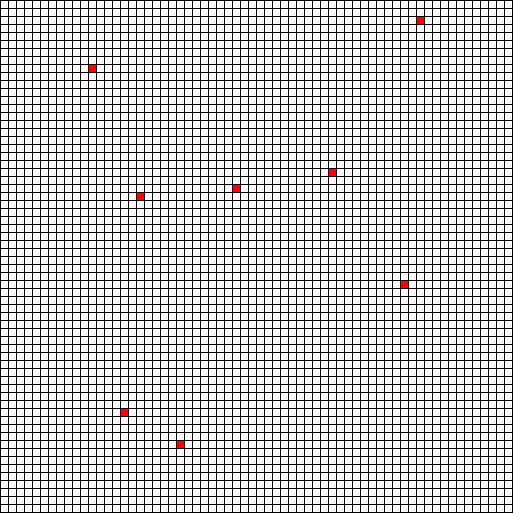
\includegraphics[height=8cm]{Old Scribe Notes/n2.png}
	\caption{Matrix $M$ which is $n^2\times n^2$ for $n=8$.}
	\label{fig:n2}
\end{figure}

\begin{figure}[ht]
	\centering
		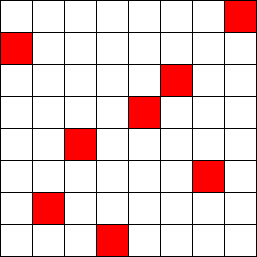
\includegraphics[height=4cm]{Old Scribe Notes/n.png}
	\caption{Matrix $M_c$ which is $n\times n$ for $n=8$. The construction worked,
	         because $M_c$ is a cycle matrix.}
	\label{fig:n}
\end{figure}


Now let's join all those probabilities. The probability that $M_c$ is a cycle matrix is at least
$$\frac{1}{3n}\cdot \frac{1}{n}\cdot \frac{1}{n} > \frac{1}{3n^3}.$$

If we repeat this process $n^4$ times, then the probability that $M_c$ is a cycle matrix in at least one iteration is at least
$$1-\left(1-\frac{1}{3n^3}\right)^{n^4}\approx 1-e^{-\frac{n}{3}} = 1-\mathsf{negl}(n).$$


\bigskip
The proof system works as follows. Given a random string $r$, the prover $P$ tries
to execute the construction above to obtain a cycle matrix.
If the construction fails, the prover simply reveals all the bits in the string $r$
to the verifier, who checks that the constructions indeed fails.
If the construction succeeds, the prover reveals all the entries in the random string $r$
that correspond to values in the matrix $M$ which are not used in matrix $M_c$.
The verifier will check that all these values for matrix $M$ are indeed 0.

Then the prover proceeds as in the previous scenario using matrix $M_c$: he
reveals the transformation $\phi$ and opens all the non-edges.

This process is repeated $n^4$ times. Or, equivalently, a big string of length
$\left\lceil 3\cdot \log_2 n\right\rceil \cdot n^4\cdot n^4$ is used and they are all
executed together. This produces a zero knowledge proof.

\textit{Completeness:} if $P$ knows the Hamiltonian cycle of $G$,
then he will be able to find a suitable transformation $\phi$ whenever a cycle graph is
generated by the construction.

\textit{Soundness:} if $P$ is lying and trying to prove a false statement, then he will
get caught with very high probability. If any of the $n^4$ iterations produces a cycle
graph, then $P$ will be caught. So the probability that he will be caught is
$1-e^{-\frac{n}{3}} = 1-\mathsf{negl}(n)$.

\textit{Zero Knowledge:} again $V$ cannot get any information if the construction succeeds.
And if the construction doesn't succeed, all $V$ gets is the random string $r$, which also
doesn't give any information.
\qed


\begin{theorem}
For any language $L$ in $NP$, there is a non-interactive zero-knowledge (NIZK) proof
in the hidden-bit model (HBM) for the language $L$.
\end{theorem}
\proof
The language $L^*$ of Hamiltonian graphs is $NP$-complete. So any problem in $L$ can
be reduced to a problem in $L^*$. More precisely, there is a polynomial-time function
$f$ such that
$$x\in L \Longleftrightarrow f(x)\in L^*.$$
So given an input $x$, the prover can simply calculate $f(x)$ and
produce a NIZK proof in the hidden-bit model for the fact that $f(x)\in L^*$.
Then the verifier just needs to calculate $f(x)$ and check if the proof for the fact
$f(x)\in L^*$ is correct.
\qed

\begin{theorem}\label{the:NIZK_NP}
For any language $L$ in $NP$, there is a non-interactive zero-knowledge (NIZK) proof
in the common reference string (CRS) model for the language $L$.
\end{theorem}
\proof
In Theorem~\ref{thm:NIZK-amplify} it was shown that any NIZK proof in the hidden-bit model can
be converted into a NIZK proof in the standard (common reference string) model by using
a trapdoor permutation.
\qed

\section{zkSNARKs}
\section*{Exercises}
\begin{exercise}[Leaky ZK proof] Formally define:
\begin{enumerate}
  \item 
What it means for an  interactive proof $(P,V)$ to be \textbf{first-bit leaky} zero-knowledge, where we require that the protocol doesn't leak anything more than the first bit of the witness.

\item What it means for an  interactive proof $(P,V)$ to be \textbf{one-bit leaky} zero-knowledge, where we require that the protocol doesn't leak anything more than one bit that is an arbitrary adversarial chosen function of the witness.
    \end{enumerate}
\end{exercise}

\begin{exercise}[Proving OR of two statements] Give a statistical zero-knowledge proof system $\Pi = (P,V)$ (with efficient prover) for the following language.
    \[ L = \left\{((G_0,G_1),(G_0',G_1'))\left| G_0 \simeq G_1 \bigvee G_0' \simeq G_1'\right.\right\}\]\\
    \textbf{Caution:} Make sure the verifier doesn't learn which of the two pairs of graphs is isomorphic.
\end{exercise}

\begin{exercise} [ZK implies WI] Let $L \in NP$ and let $(P,V)$ be an interactive proof system for $L$. We say that $(P,V)$ is \emph{witness indistinguishable (WI)} if for all PPT $V^*$, for all $x \in L$, distinct witnesses $w_1, w_2 \in R_L(x)$ and  auxiliary input $z\in \binset{*}$, the following two views are computationally indistinguishable:
\[View_{V^*} \left(P(x,w_1) \leftrightarrow V^*(x,z) \right) \simeq_c View_{V^*} \left(P(x,w_2) \leftrightarrow V^*(x,z) \right).\]
\begin{enumerate}
\item Show that if $(P,V)$ is an efficient prover zero-knowledge proof system, then it is also witness indistinguishable.

\item Assume $(P,V)$ is an efficient prover zero-knowledge proof system. We have seen in the exercise that $(P,V)$ is also witness indistinguishable. Define $(\tilde P, \tilde V)$ to repeat $(P,V)$ independently for $k$ times \emph{in parallel} ($k$ is a polynomial), and $\tilde V$ accepts if and only if $V$ accepts in all the executions. Prove that $(\tilde P, \tilde V)$ is still witness indistinguishable.
\end{enumerate}    
\end{exercise}

\begin{exercise}
\textbf{Multi-statement NIZK.} The NIZK proof system we constructed in class required a fresh common random string (CRS) for each statement proved. In various settings we would like to reuse the same random string to prove multiple theorem statements while still preserving the zero-knowledge property.
    
    A multi-statement NIZK proof system $(K,P,V)$ for a language $L$ with corresponding relation $R$ is a NIZK proof system for $L$ with a stronger zero-knowledge property, defined as follows: $\exists$ a PPT machine $\mathcal{S} = (\mathcal{S}_1,\mathcal{S}_2)$ such that $\forall$ PPT machines $A_1$ and $A_2$ we have that:
    \[\left|\Pr\left[\begin{split}\sigma \gets K(1^\kappa),\\ (\{x_i,w_i\}_{i \in [q]},\textsf{state}) \gets A_1(\sigma),\\ \text{ such that } \forall i \in [q], (x_i,w_i)\in R\\\forall i \in [q],  \pi_i \gets P(\sigma, x_i,w_i);\\
    A_2(\textsf{state}, \{\pi_i\}_{i \in [q]}) =1\end{split}\right]
    -
    \Pr\left[\begin{split}(\sigma,\tau) \gets \mathcal{S}_1(1^\kappa),\\ (\{x_i,w_i\}_{i \in [q]},\textsf{state}) \gets A_1(\sigma),\\\text{ such that } \forall i \in [q], (x_i,w_i)\in R\\\forall i \in [q],  \pi_i \gets \mathcal{S}_2(\sigma, x_i,\tau);\\ A_2(\textsf{state}, \{\pi_i\}_{i \in [q]})=1\end{split}\right]\right|
    \leq \textsf{negl}(\kappa).
    \]
    
    Assuming that a single statement NIZK proof system $(K,P,V)$ for NP exists, construct a multi-statement NIZK proof system $(K',P',V')$ for NP.\\
\textbf{Hint:} Let $g: \{0,1\}^\kappa \rightarrow \{0,1\}^{2\kappa}$ be a length doubling PRG. Let $K'$ output the output of $K$ along with $y$, a random $2\kappa$ bit string. To prove $x \in L$ the prover $P'$ proves that $\exists (w,s)$ such that either $(x,w)\in R$ or $y = g(s)$.
\end{exercise}






\newcommand{\proofsketch}{\smallskip\noindent{\bf Proof sketch. }}
\algrenewcommand\algorithmicfunction{\textbf{Machine}}
\newcommand{\bits}{\set{0,1}}
\newcommand{\Ex}{\mathbb{E}}

\renewcommand{\O}{\ensuremath{\mathcal{O}}}
\newcommand{\To}{\rightarrow}
\newcommand{\e}{\epsilon}
\newcommand{\R}{\mathbb{R}}
\newcommand{\N}{\mathbb{N}}
\newcommand{\Z}{\mathbb{Z}}
\newcommand{\logAnd}{\wedge}

\newcommand{\indis}{\mathrel{\overset{\makebox[0pt]{\mbox{\normalfont\tiny c}}}{\approx}}}
\newcommand{\allindis}{\mathrel{\overset{\makebox[0pt]{\mbox{\normalfont\tiny p/s/c}}}{\approx}}}

\newcommand{\cclass}[1]{\mathsf{#1}}
\renewcommand{\P}{\cclass{P}}
\newcommand{\NP}{\cclass{NP}}
\newcommand{\Time}{\cclass{Time}}
\newcommand{\BPP}{\cclass{BPP}}
\newcommand{\Size}{\cclass{Size}}
\newcommand{\Ppoly}{\cclass{P_{/poly}}}
\newcommand{\CSAT}{\ensuremath{\mathsf{CSAT}}}
\newcommand{\SAT}{\ensuremath{\mathsf{3SAT}}}
\newcommand{\IS}{\mathsf{INDSET}}



\newcommand{\inp}{\mathsf{in}}
\newcommand{\outp}{\mathsf{out}}

\newcommand{\Param}{\kappa}
\newcommand{\Adv}{\mathsf{Adv}}
\newcommand{\Supp}{\mathsf{Supp}}


\newcommand{\PRG}{\mathsf{G}}
\renewcommand{\Enc}{\mathsf{Enc}}
\renewcommand{\Dec}{\mathsf{Dec}}
\renewcommand{\sk}{\mathsf{sk}}
\newcommand{\sfC}{\mathsf{C}}
\newcommand{\sfR}{\mathsf{R}}

\newcommand{\eqdef}{\stackrel{\text{\tiny def}}{=}}

\newcommand{\cF}{\mathcal{F}}

\newcommand{\angles}[1]{\langle #1 \rangle}
\newcommand{\iprod}[1]{\angles{#1}}

\newcommand{\Com}{\mathsf{Com}}


% Real vs. Ideal
\newcommand{\RealAdv}{\mathcal{A}}
\newcommand{\IdealAdv}{\mathcal{S}}
\newcommand{\RealVar}{\mathsf{Real}}
\newcommand{\IdealVar}{\mathsf{Ideal}}

% Participating parties
\newcommand{\PartyA}{P_1}
\newcommand{\PartyB}{P_2}
\newcommand{\InputA}{x_1}
\newcommand{\InputB}{x_2}


% Garbling Schemes
\newcommand{\Garble}{\mathsf{Garble}}
\newcommand{\Cir}{C}
\newcommand{\GCir}{\widetilde{C}}
\newcommand{\Lab}{\mathsf{lab}}

% Proof
\newcommand{\Sim}{\mathsf{Sim}}

% GMW

% Misc
\newcommand{\out}{\mathsf{out}}
\newcommand{\Assign}{:=}

\chapter{Secure Computation}

\section{Introduction}
Secure multiparty computation considers the problem of different parties
computing a joint function of their separate, private inputs without revealing
any extra information about these inputs than that is leaked by just the result
of the computation. This setting is well motivated, and captures many different
applications. Considering some of these applications will provide intuition
about how security should be defined for secure computation:
\begin{description}
  \item[Voting:] Electronic voting can be thought of as a multi party computation
	  between $n$ players: the voters. Their input is their choice $b \in \{0,1\}$
    (we restrict ourselves to the binary choice setting without loss of generality), and the function
    they wish to compute is the majority function.

    Now consider what happens when only one user votes: their input is trivially
    revealed as the output of the computation. What does privacy of inputs mean
    in this scenario?

  \item[Searchable Encryption:] Searchable encryption schemes allow clients
    to store their data with a server, and subsequently grant servers tokens
    to conduct specific searches. However, most schemes do not consider access
    pattern leakage. This leakage tells the server potentially valuable information
    about the underlying plaintext. How do we model all the different kinds
    information that is leaked?
\end{description}

From these examples we see that defining security is tricky, with lots of
potential edge cases to consider. We want to ensure that no party can learn
anything more from the secure computation protocol than it can from just its
input and the result of the computation. To formalize this, we adopt the
\textbf{real/ideal paradigm}.



\section{Real/Ideal Paradigm}
\paragraph{Notation.} 
Suppose there are $n$ parties, and party $P_i$ has access to some data $x_i$. They are trying to compute some function of their inputs $f(x_1, \dotsc, x_n)$. The goal is to do this securely: even if some parties are corrupted, no one should learn more than is strictly necessitated by the computation.

\paragraph{Real World.} In the real world, the $n$ parties execute a protocol $\Pi$
to compute the function $f$. This protocol can involve multiple rounds of
interaction. %Each party can additionally have some randomness.
The real world adversary $\RealAdv$ can corrupt arbitrarily many (but not all) parties.


\paragraph{Ideal World.} In the ideal world, an angel helps in the
computation of $f$:
each party sends their input to the angel and receives the output of the computation $f(x_1, \dotsc, x_n)$.
Here the ideal world adversary $\IdealAdv$ can again corrupt arbitrarily many (but not all) parties.

To model malicious adversaries, we need to modify the ideal world model as follows. 
Some parties are honest, and each honest party $P_i$ simply sends $x_i$ to the angel. The other parties are corrupted and are under control of the adversary $\IdealAdv$. The adversary chooses an input $x_i'$ for each corrupted party $P_i$ (where possibly $x_i' \neq x_i$) and that party then sends $x_i'$ to the angel. The angel computes a function $f$ of the values she receives (for example, if only party 1 is honest, then the angel computes $f(x_1, x_2', x_3', \dotsc, x_n')$) in order to obtain a tuple $(y_1, \dotsc, y_n)$. 
She then sends $y_i$ of corrupted parties to the adversary, who gets to decide whether or not honest parties will receive their response from the angel. The angel obliges. Each honest party $P_i$ then outputs $y_i$ if they receive $y_i$ from the angel and $\perp$ otherwise, and corrupted parties output whatever the adversary tells them to. 

 



\paragraph{Definition of Security.} 
A protocol $\Pi$ is secure against computationally bounded adversaries if for every PPT adversary $\RealAdv$ in the real world, there exists an PPT adversary $\IdealAdv$ in the ideal world such that for all tuples of bit strings $(x_1, \dotsc, x_n)$, we have
\[ \mathrm{Real}_{\Pi, \RealAdv}(x_1, \dotsc x_n) \stackrel{c}{\simeq} \mathrm{Ideal}_{F,\IdealAdv}(x_1, \dotsc, x_n) \]
where the left-hand side denotes the output distribution induced by $\Pi$ running with $\RealAdv$, and the right-hand side denotes the output distribution induced by running the ideal protocol $F$ with $\IdealAdv$. 
The ideal protocol is either the original one described for semi-honest adversaries, or the modified one described for malicious adversaries. 





%We require that the views of the parties
%in each of the scenarios be identical, i.e.\ that a real-world execution of the
%protocol $\Pi$ should not leak any information not leaked by the ideal-world
%execution. Hence, the parties can only learn what they can infer from their
%inputs and the output $f(\InputA, \InputB)$. More formally, assuming $\RealAdv$
%corrupts one party (say $\PartyA$, wlog), we define random variables
%$\RealVar_{\Pi, \RealAdv}(\InputA, \InputB) = \RealAdv(\InputA, r_1, \text{messages
%sent in } \Pi)$ and $\IdealVar_{F, \IdealAdv}(\InputA, \InputB) = \IdealAdv(\InputA,
%f(\InputA,\InputB))$.  These random variables represent the views of the
%adversary in each of the two settings. Our definition of security thus requires
%that
%
%\begin{equation*}
%\RealVar_{\Pi, \RealAdv}(\InputA, \InputB) \indis \IdealVar_{F, \IdealAdv}(x_1, x_2).
%\end{equation*}

\paragraph{Assumptions.} We have brushed over some details of the above setting.
Below we state these assumptions explicitly:
\begin{enumerate}
  \item \textbf{Communication channel:} We assume that the communication channel
    between the involved parties is completely insecure, i.e., it does not preserve
    the privacy of the messages. However, we assume that it is reliable, which means
    that the adversary can drop messages, but if a message is delivered, then
    the receiver knows the origin.

  \item \textbf{Corruption model:} We have different models of how and when the
    adversary can corrupt parties involved in the protocol:
    \begin{itemize}
      \item
        \emph{Static:} The adversary chooses which parties to corrupt before the
        protocol execution starts, and during the protocol, the malicious parties
        remain fixed.
      \item
        \emph{Adaptive:} The adversary can corrupt parties dynamically during
        the protocol execution, but the simulator can do the same.
      \item
        \emph{Mobile:} Parties corrupted by the adversary can be ``uncorrupted''
        at any time during the protocol execution at the adversary's discretion.
    \end{itemize}

  \item \textbf{Fairness:} The protocols we consider are not ``fair'', i.e.,
    the adversary can cause corrupted parties to abort arbitrarily. This can
    mean that one party does not get its share of the output of the computation.

  \item \textbf{Bounds on corruption:} In some scenarios, we place upper bounds
    on the number of parties that the adversary can corrupt.

  \item \textbf{Power of the adversary:} We consider primarily two types of
    adversaries:
    \begin{itemize}
      \item \emph{Semi-honest adversaries:} Corrupted parties follow the protocol
        execution $\Pi$ honestly, but attempt to learn as much information as they
        can from the protocol transcript.

      \item \emph{Malicious adversaries:} Corrupted parties can deviate arbitrarily
        from the protocol $\Pi$.
    \end{itemize}

  \item \textbf{Standalone vs.\ Multiple execution:} In some settings, protocols
    can be executed in isolation; only one instance of a particular protocol
    is ever executed at any given time. In other settings, many different protocols
    can be executed concurrently. This can compromise security.
\end{enumerate}







\section{Oblivious transfer}

\emph{Rabin's oblivious transfer} sets out to accomplish the following special task of two-party secure computation. The sender has a bit $s \in \{0,1\}$. She places the bit in a box. Then the box reveals the bit to the receiver with probability 1/2, and reveals $\perp$ to the receiver with probability 1/2. The sender cannot know whether the receiver received $s$ or $\perp$, and the receiver cannot have any information about $s$ if they receive $\perp$.

\subsection{1-out-of-2 oblivious transfer}
\emph{1-out-of-2 oblivious transfer} sets out to accomplish the following related task. The sender has two bits $s_0, s_1 \in \{0,1\}$ and the receiver has a bit $c \in \{0,1\}$. The sender places the pair $(s_0, s_1)$ into a box, and the receiver places $c$ into the same box. The box then reveals $s_c$ to the receiver, and reveals $\perp$ to the sender (in order to inform the sender that the receiver has placed his bit $c$ into the box and has been shown $s_c$). The sender cannot know which of her bits the receiver received, and the receiver cannot know anything about $s_{1-c}$.

\begin{lemma}
A system implementing 1-out-of-2 oblivious transfer can be used to implement Rabin's oblivious transfer.
\end{lemma}

\proof
The sender has a bit $s$. She randomly samples a bit $b \in \{0,1\}$ and $r \in \{0,1\}$, and the receiver randomly samples a bit $c \in \{0,1\}$. If $b = 0$, the sender defines $s_0 = s$ and $s_1 = r$, and otherwise, if $b = 1$, she defines $s_0 = r$ and $s_1 = s$. She then places the pair $(s_0, s_1)$ into the 1-out-of-2 oblivious transfer box. The receiver places his bit $c$ into the same box, and then the box reveals $s_c$ to him and $\perp$ to the sender. Notice that if $b = c$, then $s_c = s$, and otherwise $s_c = r$. Once $\perp$ is revealed to the sender, she sends $b$ to the receiver. The recieiver checks whether or not $b = c$. If $b = c$, then he knows that the bit revealed to him was $s$. Otherwise, he knows that the bit revealed to him was the nonsense bit $r$ and he regards it as $\perp$. \\

It is easy to see that this procedure satisfies the security requirements of Rabin's oblivious transfer protocol. Indeed, as we saw above, $s_c = s$ if and only if $b = c$, and since the sender knows $b$, we see that knowledge of whether or not the bit $s_c$ received by the receiver is equal to $s$ is equivalent to knowledge of $c$, and the security requirements of 1-out-of-2 oblivious transfer prevent the sender from knowing $c$. Also, if the receiver receives $r$ (or, equivalently, $\perp$), then knowledge of $s$ is knowledge of the bit that was not revealed to him by the box, which is again prevented by the security requirements of 1-out-of-2 oblivious transfer.  $\qed$

\begin{lemma}
A system implementing Rabin's oblivious transfer can be used to implement 1-out-of-2 oblivious transfer.
\end{lemma}

\proofsketch
The sender has two bits $s_0, s_1 \in \{0,1\}$ and the receiver has a single bit $c$. The sender randomly samples $3n$ random bits $x_1, \dotsc, x_{3n} \in \{0,1\}$. Each bit is placed into its own a Rabin oblivious transfer box. The $i$th box then reveals either $x_i$ or else $\perp$ to the receiver. Let 
\[ S := \{i \in \{1, \dotsc, 3n\} : \text{the receiver knows } x_i\}. \]
The receiver picks two sets $I_0, I_1 \subseteq \{1, \dotsc, 3n\}$ such that $\# I_0 = \# I_1 = n$, $I_c \subseteq S$ and $I_{1-c} \subseteq \{1, \dotsc, 3n\} \setminus S$. This is possible except with probability negligible in $n$. He then sends the pair $(I_0, I_1)$ to the sender. The sender then computes $t_j= \left(\bigoplus_{i \in I_j}x_i \right) \oplus s_j$ for both $j \in \{0,1\}$ and sends $(t_0, t_1)$ to the receiver. \\

Notice that the receiver can uncover $s_c$ from $t_c$ since he knows $x_i$ for all $i \in I_c$, but cannot uncover $s_{1-c}$. One can show that the security requirement of Rabin's oblivious transfer implies that this system satisfies the security requirement necessary for 1-out-of-2 oblivious transfer. $\qed$ \\

We will see below that length-preserving one-way trapdoor permutations can be used to realize 1-out-of-2 oblivious transfer. 

\begin{theorem}
The following protocol realizes 1-out-of-2 oblivious transfer in the presence of computationally bounded and semi-honest adversaries. 
\begin{enumerate}
\item The sender, who has two bits $s_0$ and $s_1$, samples a random length-preserving one-way trapdoor permutation $(f, f^{-1})$ and sends $f$ to the receiver.  Let $b(\cdot)$ be a hard-core bit for $f$.
\item The receiver, who has a bit $c$, randomly samples an $n$-bit string $x_c \in \{0,1\}^n$ and computes $y_c = f(x_c)$. He then samples another random $n$-bit string $y_{1-c} \in \{0,1\}^n$, and then sends $(y_0, y_1)$ to the sender.
\item The sender computes $x_0 := f^{-1}(y_0)$ and $x_1 := f^{-1}(y_1)$. She computes $b_0 := b(x_0) \oplus s_0$ and $b_1 := b(x_1) \oplus s_1$, and then sends the pair $(b_0, b_1)$ to the receiver.
\item The receiver knows $c$ and $x_c$, and can therefore compute $s_c = b_c \oplus b(x_c)$. 
\end{enumerate}
\end{theorem}
\proof
Correctness is clear from the protocol.	
For security, from the sender side, since $f$ is a length-preserving permutation, $(y_0, y_1)$ is statistically indistinguishable from two random strings, hence she can't learn anything about $c$.
From the receiver side, guessing $s_{1-c}$ correctly is equivalent to guessing the hard-core bit for $y_{1-c}$.
\qed


\subsection{1-out-of-4 oblivious transfer}
  We describe how to implement a 1-out-of-4 OT using 1-out-of-2 OT:\@
  \begin{enumerate}
    \item
      The sender, $\PartyA$ samples 5 random values $S_i \gets \bits, i \in \set{1,\dotsc, 5}$.
    \item
      $\PartyA$ computes
      \begin{align*}
        \alpha_0 &= S_0 \xor S_2 \xor m_0\\
        \alpha_1 &= S_0 \xor S_3 \xor m_1\\
        \alpha_2 &= S_1 \xor S_4 \xor m_2\\
        \alpha_3 &= S_1 \xor S_5 \xor m_3
      \end{align*}
      It sends these values to $\PartyB$.
    \item
      The parties engage in 3 1-out-of-2 Oblivious Transfer protocols for the following
      messages: $(S_0, S_1)$, $(S_2, S_3)$, $(S_4, S_5)$. THe receiver's input for
      the first OT is the first choice bit, and for the second and third ones is
      the second choice bit.
    \item
      The receiver can only decrypt one ciphertext.
  \end{enumerate}

\section{Yao's Garbled Circuit}


%\input{HWsolution.tex}
%\part{Yao's Garbled Circuit}

% ===========
\section{Setup}


Yao's Garbled Circuits is presented as a solution to Yao's Millionaires' problem, 
which asks whether 
two millionaires can compete for bragging rights of which is richer
without revealing their wealth to each other. 
It started the area of secure computation. 
We will present a solution for the two party problem;
it can be extended to a polynomial number of parties,
using the techniques from last lecture.

The solution we saw previously needed an interaction for each AND gate.
Yao's solution requires only one message,
so it provides a constant size of interaction.
We present a solution only for semi honest security. 
This can be amplified to malicious security, 
but there are more efficient ways of amplifying this than what we saw last lecture.

\subsection{Secure Computation}

Recall our definition of secure computation. 
We define ideal and real worlds. 
Security is defined to hold if 
anything an attacker can achieve in the real world 
 can also be achieved by an ideal attacker in the ideal world. 
We define the ideal world to have the properties that we desire. 
For security to hold these properties must also hold in the real world.

\subsection{$(\Garble, \Eval)$}
We will provide a definition, similar to how we define encryption, that allows us avoid dealing with simulators all the time. 


Yao's Garbled Circuit is defined as two efficient algorithms $(\Garble, \Eval)$. Let the circuit $C$ have $n$ input wires.
$\Garble$ produces the garbled circuit and two labels for each input wire. The labels are for each of 0 and 1 on that wire and are like encryption keys. 

\[
(\tilde{C}, \{\ell_{i,b}\}_{i \in [n], b \in \{0,1\}}) \leftarrow \Garble(1^k, C) 
\]

To evaluate the circuit on a single input we must choose a value for each of the n input wires.
Given n of 2n input keys, $\Eval$ can evaluate the circuit on those keys and get the circuit result.
\[
C(x) \leftarrow \Eval(\tilde{C}, \{\ell_{i, x_i}\}_{i \in [n]}) 
\]

\paragraph{Correctness}
Correctness is as usual, if you garble honestly, evaluation should produce the correct result. 
\[
\forall C, x 
Pr[ C(x) = \Eval(\tilde{C}, \{l_{i, x_i}\}),  (\tilde{C}, \{\ell_{i,b}\}) = \Garble(1^k, C)] = 1 - neg(k)
\]


\paragraph{Security}
For security we require that a party receiving 
a garbled circuit and n inputs labels 
can not computationally distinguish the joint distribution of the circuits and labels
from the distribution produced by 
a simulator with access to the circuit and its evaluation on the input that the labels represent. 
The simulator does not have access to the actual inputs.
If this holds, the party receiving the garbled circuit and n labels can not determine the inputs.

\begin{align*}
&\exists \Sim : \forall C, x\\
&(\tilde{C}, \{\ell_{i,x_i}\}_{i \in [n]}) \simeq \Sim(1^k, C, C(x)) \text{ where} \\
&(\tilde{C}, \{\ell_{i,b}\}_{i \in [n], b \in \{0,1\}}) \leftarrow \Garble(1^k, C) 
\end{align*}

For simplicity we pass the circuit to the simulator.
You could also use universal circuits and pass 
in with the inputs the specific circuit that the universal circuit should realize. 



\section{Use for Semi-honest two party secure communication}
Alice, with input $x^1$, and Bob, with input $x^2$, have a circuit, C, that they want to evaluate securely. 
The size of their combined inputs is n, so $|x^1| = n_1, |x^2| = n - n_1, |x^1| + |x^2| = n$.
They can do this by Alice garbling a circuit and sending input wire labels to Bob, as in Figure \ref{fig:message}.

Alice garbles the circuit and passes it to Bob, $\tilde{C}$.
Alice passes the labels for her input directly to Bob, $\{\ell_{i, x^1_i}\}_{i \in [n] / [n_2]}$.
Alice passes all the labels for Bob's input wires into oblivious transfer, $\{\ell_{i, b_i}\}_{i \in [n] / [n_1], b \in \{0,1\}}$, 
from which Bob can retrieve the labels for his actual inputs, $\{\ell_{i, x^2_i}\}_{i \in [n] / [n_1]}$.
Bob now has the garbled circuit and one label for each input wire. 
He evaluates the garbled circuit on those garbled inputs and learns $C(x^1||x^2)$.
Bob does not learn anything besides the result as he has only the garbled circuit and n garbled inputs.
Alice does not learn anything as she uses oblivious transfer to give Bob his input labels and receives nothing in reply.

\begin{figure}[htbp]
\begin{center}
\setlength{\unitlength}{1cm}
\begin{picture}(10, 7)(-5, -4)
% \put(-.5,2){\makebox(1,1){C}}
 \put(-6,2){\makebox{Alice: $C, x^1$}}
 \put(-6,1.3){\makebox{$(\tilde{C}, \{\ell_{i,b}\}) \leftarrow \Garble$}}
 \put(4,2){\makebox{Bob: $C, x^2$}}

 \put(-1,0){\makebox(2,2){$\underrightarrow{\tilde{C}}$}}
  \put(-1,-0.8){\makebox(2,2){$\underrightarrow{ S_{out}^0 \text{ is 0 }, S_{out}^1 \text{ is 1 } }$}}


 \put(-1,-2){\makebox(2,2){$\underrightarrow{\{\ell_{i, x^1_i}\}_{i \in [n] / [n_2]}}$}}
% \put(-1,-1){\makebox(2,2){$\underrightarrow{\ell_{i,0}, \, \ell_{i,1} \forall i \in  [n]/[n_1] }$}}

 \put(-.5,-3){\framebox(1,1){OT}}
  \put(-1,-2.8){\line(1,0){.5}}
   \put(-1.6,-2.8){\makebox{$\ell_{i,1}$}}

  \put(-1,-2.2){\line(1,0){.5}}
     \put(-1.6,-2.2){\makebox{$\ell_{i,0}$}}

  \put(.5,-2.5){\line(1,0){.5}}
     \put(1.2,-2.5){\makebox{$\{\ell_{i, x^2_i}\}_{i \in [n] / [n_1]}$}}
     
  \put(-1,-4.5){\makebox(2,2){$\underrightarrow{ \forall i \in  [n]/[n_1] }$}}


\end{picture}
\caption{Messages in Yao's Garbeled Circuit}
\label{fig:message}
\end{center}
\end{figure}






%\paragraph{Malicious Bob}
%Alice semi-honest, and oblivious transfer is maliciously secure.
%Holds against malicious $Bob^*$
% What of deliberate circuit that shows first input  

\subsection{Construction of Garbled Circuits}

We would like to garble a circuit such that there are two keys for each input wire.
Correctness should be that 
given one of the two keys for each wire we can compute the output for the inputs those keys correspond to.
Security should be that 
given one key for each wire you can only learn the output, not the actual inputs.

%---

We build the circuit as a bunch of NAND gates that outputs one bit. 
If more bits are required, this can be done multiple times.
NAND gates can create any logic needed. 
We define the following sets:
\begin{align*}
W &= \text{the set of wires in the circuit}\\
G &= \text{the set of gates in the circuit.}
\end{align*}

For  each wire in the circuit, sample two keys
to label the possible inputs $0$ and $1$  to the wire
\[
\forall w \in W  \quad S_w^0, S_w^1 \,  \leftarrow{} \{0,1\}^k.
\]
We can think of these as the secret keys to an encryption scheme
(Gen, Enc, Dec).
For such a scheme we can always replace the secret key with the random bits fed into Gen.


\paragraph{Wires}
For each wire in the circuit we will have an invariant that the evaluator can only get one of the wires two encrypted values.
Consider an internal wire fed by the evaluation of a gate. The gate receives two encrypted values as inputs
and produces one encrypted output. The output will be one of the two labels for that wire and the evaluator will have no 
way of obtaining the other label for that wire. 
For example on wire $w_i$, the evaluator will only learn the value for $1$,  $S_{w_i}^1$.
We ensure this for the input wires by giving the evaluator only one of the two encrypted values for the wire.

\paragraph{Gates}
For every gate in the circuit we create four cipher texts. 
For each choice of inputs we encrypt the output key under each of the input keys. 
Let gate $g$ have inputs $w_1, w_2$ and output $w_3$,
\begin{align*}
e_g^{00} &= \Enc_{S_{w_1}^0} ( \Enc_{S_{w_2}^0}  ( S_{w_3}^1, 0^k) )\\
e_g^{01} &= \Enc_{S_{w_1}^0} ( \Enc_{S_{w_2}^1}  ( S_{w_3}^1, 0^k) )\\
e_g^{10} &= \Enc_{S_{w_1}^1} ( \Enc_{S_{w_2}^0}  ( S_{w_3}^1, 0^k) )\\
e_g^{11} &= \Enc_{S_{w_1}^1} ( \Enc_{S_{w_2}^1}  ( S_{w_3}^0, 0^k) ).
\end{align*}
We add $k$ zeros at the end.

\paragraph{Final Output}
For the final output wire, $S_{out}$, we can just give out their values,
\begin{align*}
S_{out}^0 &\text{ corresponds to 0}\\
S_{out}^1 &\text{ corresponds to 1.}
\end{align*}

\paragraph{$\bold{\tilde{C}}$}
For each gate, Alice sends Bob a random permutation of the set of four encrypted output values.
\[
\{e_g^{C_1, C_2} \} \quad \forall g \in G \quad C_1, C_2 \in \{0,1\}.
\]
For each gate, Alice sends Bob a random permutation of the set of four encrypted output values

\paragraph{Evaluation}
With an encrypted gate $g$,
input keys $S_{w_1} \, S_{w_2}$ for the input wires,
and four randomly permuted encryptions of the output keys, $e_g^{a}, e_g^{b}, e_g^{c}, e_g^{d}$,
Bob can evaluate the gate to find the corresponding key $S_{w3}$ for the output wire.
Bob can decrypt each of the encrypted output keys until he finds one that decrypts 
to a string ending in the proper number of $0$'s, which is very likely to contain the proper output key.
We can increase the probability of the correct key by increasing the number of $0$'s. 
\[
\exists  i \in \{a, b, c, d\} : \Dec_{S_{w_2}} ( \Dec_{S_{w_1}} ( e_g^{i} ))  = S_{w_3}, 0^k
\]

Given input wire labels 
$\{ \ell_{i, x_i} \}_{i \in [n]}$
the complete encrypted circuit $\tilde{C}$ is evaluated by working up from the input gates. 

%$l_{i,b} = \{S_{i,b}\}$

%as with PRF encryption scheme
%$Enc(_s(m) = (r,  m \oplus F_s(r)$


The evaluator should not be able to infer anything except what they could infer in the ideal world.
As a simple example, if the evaluator supplies one input to a circuit of just one NAND gate,
 they would be able to infer the input of the other party. However, this is true is the ideal world as well.

\section{Proof Intuition}

What intuition can we offer that the 
distribution of $\tilde{C}$ with one label per input wire 
is indistinguishable from what which a simulator could produce with access to the output?
%
For each input wire we are only given one key.
As we are doing double encryption,
for each input gate we only have the keys needed to decrypt one of the four possible outputs.
The other three are protected by semantic security.
%
So from each input gate we learn only one key compounding to its output wire.
As the output labels were randomized, we also do not know if that key corresponds to a 0 or a 1. 
%
For the next level of gates we again have only one key per input wire, and our argument continues. 
%
 So for each wire of the circuit we can only know one key corresponding to an output value for the wire. 
 Everything else is random garbage.
% 
As we control the mapping from output keys to output values, we can set this to whatever is needed to
match the expected output. 


Security only holds for evaluation of the circuit with one set of input values and 
we assume that the circuit is combinatorial and thus acyclic. 

% with two input all 0 or all 1 all broken
%  even with just 2 keys for one  input wire - broken. 


% !TEX root = collection.tex

\section{Malicious attacker intead of semi-honest attacker}

The assumption we had before consisted of a semi-honest attacker instead of a malicious attacker. A malicious attacker does not have to follow the protocol, and may instead alter the original protocol. The main idea here is that we can convert a protocol aimed at semi-honest attackers into one that will work with malicious attackers.

At the beginning of the protocol, we have each party commit to its inputs:
Given a commitment protocol $com$, Party 1 produces
\begin{center}
$c_1 = com(x_1; w_1)$ \\
$d_1 = com(r_1; \phi_1)$ \\
\end{center}
Party 2 produces
\begin{center}
$c_2 = com(x_2; w_2)$\\
$d_2 = com(r_2; \phi_2)$
\end{center}

We have the following guarantee: $\exists x_i, r_i, w_i, \phi_i$ such that $c_i = com(x_i; w_i) \wedge d_i = com(r_i; \phi_i) \wedge t = \pi(i,\text{transcript}, x_i, r_i)$, where transcript is the set of messages sent in the protocol so far.

Here we have a potential problem. Since both parties are choosing their own random coins, we have to be able to enforce that the coins are \emph{indeed} random. We can solve this by using the following protocol:

\begin{center}
  \begin{picture}(200,100)(10,20)
    \put(20, 90){$d_1 = com(s_1; \phi_1)$}
    \put(20,80){\vector(1,0){50}}
    \put(150, 90){$d_2 = com(s_2; \phi_2)$}
    \put(200, 80){\vector(-1,0){50}}

    \put(20, 60){$s_2^{'}$}
    \put(20,50){\vector(1,0){50}}
    \put(200, 60){$s_1^{'}$}
    \put(200, 50){\vector(-1,0){50}}
  \end{picture}
\end{center}

We calculate $r_1 = s_1 \oplus s_1^{'}$, and $r_2 = s_2 \oplus s_2^{'}$. As long as one party is picking the random coins honestly, both parties would have truly random coins.

Furthermore, during the first commitment phase, we want to make sure that the committing party actually knows the value that is being committed to. Thus, we also attach along with the commitment a zero-knowledge proof of knowledge (ZK-PoK) to prove that the committing party knows the value that is being committed to.

\subsection{Zero-knowledge proof of knowledge (ZK-PoK)}

\begin{definition}[ZK-PoK] Zero-knowlwedge proof of knowledge (ZK-PoK) is a zero-knowledge proof system $(P,V)$ with the property proof of knowledge with knowledge error $\kappa$:

$\exists$ a PPT $E$ (knowledge extractor) such that $\forall x \in L$ and $\forall P^{*}$ (possibly unbounded), it holds that if $\Pr[Out_V(P^{*}(x,w) \leftrightarrow V(x))]> \kappa(x)$, then 
\[ \Pr[E^{P^*}(x) \in R(x)] \geq \Pr[Out_V(P^{*} \leftrightarrow V(x))] = 1]- \kappa(x).\]
Here we have $L$ be the language, $R$ be the relation, and $R(x)$ is the set such that $\forall w \in R(x)$, $(x, w) \in R$.
\end{definition}

Given a zero-knowledge proof system, we can construct a ZK-PoK system for statement $x\in L$ with witness $w$ as follows:
\begin{center}
  \begin{picture}(300,300)(10,20)

    \put(10, 290){$P$}
    \put(290, 290){$V$}

    \put(10, 270){$r \leftarrow \{0, 1\}^{|w|}$}

    \put(100, 260){$c_1 = com(r; \omega)$}
    \put(100, 250){$c_2 = com(r \oplus w; \phi)$}
    \put(100, 240){\vector(1,0){100}}

    \put(150, 210){$b$}
    \put(200, 200){\vector(-1,0){100}}

    \put(120, 160){if $b = 0$, open $c_1$ to reveal $r$}
    \put(120, 150){else open $c_2$ to reveal $r \oplus w$}
    \put(100, 140){\vector(1,0){100}}

    \put(120, 60){\framebox(50,50)[c]{ZK Proof}}
  \end{picture}
\end{center}

The last ZK proof proves that $\exists r, w, \omega, \phi$ such that $(x, w) \in R$ and $c_1 = com(r; \omega)$, $c_2 = com(r \oplus w; \phi)$.


\section*{Exercises}
\begin{exercise}
Given a (secure against malicious adversaries) two-party secure computation protocol (and nothing else) construct a (secure against malicious adversaries) three-party secure computation protocol.
\end{exercise}

% !TEX root = collection.tex

\chapter{Obfustopia}


\section{Witness Encryption: A Story}\label{story}

Imagine that a billionaire who loves mathematics, would like to award with 1 million dollars the mathematician(s) who will prove the Riemann Hypothesis. Of course, neither does the billionaire know if the Riemann Hypothesis is true, nor if he will be still alive (if and) when a mathematician will come up with a proof. To overcome these couple of problems, the billionaire decides to:

\begin{enumerate}

\item Put 1 million dollars in gold in a big treasure chest.

\item Choose an arbitrary place of the world, dig up a hole, and hide the treasure chest.

\item Encrypt the coordinates of the treasure chest in a message so that only the mathematician(s) who can actually prove the Riemann Hypothesis can decrypt it.

\item Publish the ciphertext in every newspaper in the world.

\end{enumerate}

The goal of this lecture is to help the billionaire with step 3. To do so, we will assume for simplicity  that the proof is at most 10000 pages long. The latter assumption implies that the language
\begin{align*}
L = \{ x \text{ such that } x \text{ is an acceptable Riemann Hypothesis proof} \}
\end{align*}
 is in NP and therefore, using a reduction, we can come up with a circuit $C$ that takes as input $x$ and outputs $1$ if $x$ is a proof for the Riemann Hypothesis and $0$ otherwise.

\smallskip
Our goal now is to  design a pair of PPT machines $(\mathrm{Enc},\mathrm{Dec})$ such that:

\begin{enumerate}
\item $\mathrm{Enc}(C,m)$ takes as input the circuit $C$ and $m \in \{0,1\}$ and outputs a ciphertext $e \in \{0,1\}^{*}$.

\item $\mathrm{Dec}(C,e,w)$ takes as input the circuit $C$, the cipertext $e$ and a witness $w \in \{0,1\}^{*}$ and outputs $m$ if if $C(w) = 1$ or $\perp$ otherwise.
\end{enumerate}

and so that they satisfy the following correctness and security requirements:

\begin{itemize}

\item \textbf{Correctness:} If $\exists w$ such that $C(w) = 1$ then $\mathrm{Dec}(C,e,w)$ outputs $m$.

\item \textbf{Security:} If $\nexists w$ such that $C(w) = 1$ then $\mathrm{Enc}(C,0)   \approx^{c} \mathrm{Enc}(C,1) \!\ $ (where $ \approx^{c}$ means  ``computationally indistinguishable'').

\end{itemize}


\section{A Simple Language }

As a first example, we show how we can design such an encryption scheme for a simple language. Let $G$ be a group of prime order and  $g$ be a generator of the group. For elements $A, B, T \in G$ consider the language $L = \{(a,b): A = g^a, B = g^b, T = g^{ab} \}$. An encryption scheme for that language with the correctness and security requirements of Section~\ref{story} is the following:

\smallskip

\begin{itemize}

\item \textbf{Encryption$(g,A,B,T,G)$:}

\begin{itemize}
\item Choose elements $r_1, r_2 \in \mathbb{Z}_p^*$ uniformly and independently.

\item Let $c_1 = A^{r_1} g^{r_2} $, $c_2 =  g^m T^{r_1} B^{r_2}$, where $m \in \{0,1\}$ is the message we want to encrypt.

\item Output $c = (c_1, c_2)$

\end{itemize}

\item \textbf{Decryption($b$):}


\begin{itemize}

\item Output $\frac{c_2}{c_1^b}$

\end{itemize}

\end{itemize}


\textbf{Correctness:}
The correcntess of the above encryption scheme follows from the fact that if there exist $(a,b) \in L$ then:

\begin{eqnarray*}
\frac{c_2}{c_1^b} & = &  \frac{g^m T^{r_1} B^{r_2}  }{ \left( A^{r_1}g^{r_2}\right)^b } \\
& = & \frac{g^m \left(g^{ab}\right)^{r_1} \left( g^{b} \right)^{r_2}  }{ \left( g^{a} \right)^{r_1 b} g^{r_2 b} } \\
& = & g^{m}
\end{eqnarray*}

Since $m \in \{0,1\}$ and we know $g$, the value of $g^m$ implies the value of $m$.

\smallskip
\textbf{Security:}
As far as the security of the scheme is concerned, since $L$ is quite simple, we can actually prove that $m$ is information-theoretically hidden. To see this, assume there does not exist $(a,b) \in L$, but an adversary has the power to compute discrete logarithms. In that case, given $c_1$ and $c_2$ the adversary could get a system of the form:
\begin{eqnarray*}
ar_1 + r_2 & = & s_1 \\
m + r r_1 + b r_2 &=& s_2
\end{eqnarray*}
where $s_1$ and $s_2$ are   the discrete logarithms of $c_1$ and $c_2$ respectively (with base $g$), and $r \ne ab$ is an element of $  \mathbb{Z}_{p}^*$ such that $T = g^r$. Observe now that for each value of $m$ there exist numbers $r_1$ and $r_2$ so that the above system has a solution, and thus $m$ is indeed information-theoretically hidden (on the other hand, if we had that $ab = r$ then the equations are linearly dependent).

\newpage
\section{An  NP Complete Language }

In this section we focus on our original goal of designing an encryption for an NP complete language $L$. Specifically, we will consider the NP-complete problem \emph{exact cover}. Besides that, we introduce the $n$-Multilinear  Decisional Diffie-Hellman ($n$-MDDH) assumption  and the Decisional Multilinear No-Exact-Cover Assumption.  %(see also~\cite{Sanjam}). 
The latter will guarantee the security of our construction.

\subsection{ Exact Cover}

We are given as input $x = (n, S_1, S_2, \ldots, S_l)$, where $n$ is an integer and each $S_i, i \in [l]$ is a subset of $[n]$, and our goal is to find a subset of indices $T \subseteq [l]$ such that:

\begin{enumerate}
\item $\cup_{i \in T} S_i = [n] $ and

\item $\forall i, j \in T$ such that $i \ne j$ we have that $S_i \cap S_j = \emptyset$.
\end{enumerate}

If such a $T$ exists, we say that $T$ is an exact cover of $x$.

\subsection{Multilinear Maps}

Mutlinear maps is a generalization of bilinear maps (which we have already seen) that will be useful in our construction. Specifically, we assume the existence of a group generator $\mathcal{G}$, which takes as input a security parameter $\lambda$ and a positive integer $n$ to indicate the number of allowed operations. $\mathcal{G}(1^{\lambda},n)$ outputs a sequence of groups $\vec{\mathbb{G}}= (\mathbb{G}_1, \mathbb{G}_2, \ldots, \mathbb{G}_n)$  each of large prime order $P > 2^{\lambda}$. In addition, we let $g_i$ be a canonical generator of $\mathbb{G}_i$  (and is known from the group's description).

We also assume the existence of a set of bilinear maps $\{e_{i,j}: \mathbb{G}_i \times \mathbb{G}_j \rightarrow \mathbb{G}_{i+j} \mid i, j \ge 1; i+j \le n \}.$ The map $e_{i,j}$ satisfies the following relation:
\begin{align}
e_{i,j}\left(g_i^{a},g_j^{b}\right) = g^{ab}_{i+j}: \forall a,b \in \mathbb{Z}_p \label{vasikoni}
\end{align}
and we observe that one consequence of this is that $e_{i,j} (g_i, g_j) = g_{i+j}$ for each valid $i,j$.

\subsection{The $n$-MDDH Assumption  }

The $n$-Multilinear Decisional Diffie-Hellman ($n$-MDDH) problem states the following: A challenger runs $\mathcal{G}(1^{\lambda},n ) $ to generate groups and generators of order $p$. Then it picks random $s, c_1, \ldots, c_n  \in \mathbb{Z}_p$.  The assumption then states that given $g= g_1, g^{s}, g^{c_1}, \ldots,g^{c_n}$ it is hard to distinguish $T = g_n^{s \prod_{j \in [1,n ] } c_j}$ from a random group element in $G_n$, with better than negligible advantage (in security parameter $\lambda$).

\newpage


\subsection{Decisional Multilinear  No-Exact-Cover  Assumption}
Let $x = (n, S_1, \ldots, S_l)$ be an instance of the exact cover problem that has no solution. Let $\mathrm{param} \leftarrow \mathcal{G}(1^{1+n},n)$ be a description of a multilinear group family with order $p = p(\lambda)$. Let $a_1, a_2, \ldots, a_n,r$ be uniformly random in $\mathbb{Z}_p$. For $i \in [l]$, let $c_i  = g_{|S_i|}^{ \prod_{j \in S_i} a_j}$. Distiguish between the two distributions:
\begin{align*}
(\mathrm{params}, c_1, \ldots,c_l,g_n^{a_1a_2\ldots a_n}) \text{ and } (\mathrm{params},c_1, \ldots,c_l,g_n^r)
\end{align*}

The Decisional Multilinear No-Exact-Cover Assumption is that for all adversaries $\mathcal{A}$, there exists a fixed negligible function $\nu(\cdot)$ such that for all instances $x$ with no solution, $\mathcal{A}$'s distinguishing advantage against the Decisional Multilinear No-Exact-Cover Problem  for $x$ is at most $\nu(\lambda)$.

\subsection{The Encryption Scheme  }

We are now ready to give the description of our encryption scheme.

\begin{itemize}

\item $\mathrm{Enc}(x,m)$ takes as input $x=(n, S_1, \ldots,S_l)$ and the message $m \in \{0,1\}$ and:

\begin{itemize}

\item Samples $a_{0}, a_1, \ldots, a_{n}$ uniformly and independently from $\mathbb{Z}_p^*$.

\item $\forall i \in [l]$ let $c_i = g^{\prod_{j\in S_j} a_j}_{|S_i|}$

\item Sample uniformly an element $r \in \mathbb{Z}_p^*$

\item Let $d = d(m) $ be $  g_n^{\prod_{j \in [n]}a_j}$ if $m = 1 $ or $g_n^r$ if $m = 0$.

\item Output $c = (d, c_1, \ldots,c_l)$
\end{itemize}

\item $\mathrm{Dec}(x,T)$, where $T \subseteq[l]$ is a set of indices, computes $\prod_{i \in T}c_i$ and outputs $1$ if the latter value equals to $d$ or $0$ otherwise.

\end{itemize}


\begin{itemize}

\item \textbf{Correctness:} Assume that $T$ is an exact cover of $x$. Then, it is not hard to see that:
\begin{eqnarray*}
\prod_{i \in T} c_i & = & \prod_{i \in T} g^{\prod_{j\in S_j} a_j}_{|S_i|} \\
& = & g_n^{\prod_{j \in [n]}a_j}
\end{eqnarray*}
where we have used~\eqref{vasikoni} repeatedly and the fact that $T$ is an exact cover (to show that $\sum_{i \in T} |S_i| = n$ and that $\prod_{i \in T} \prod_{j \in S_i} a_j = \prod_{i \in [n]} a_i$).

\item \textbf{Security:} Intuitively, the construction is secure, since the only way to make $g_n^{\prod_{ j \in [n] }a_i}$ is to find an exact cover of $[n]$.  As a matter of fact, observe that if an exact cover does not exist, then for each subset of indices $T'$( such that $\cup_{i \in T'}S_j  = [n]$) we have that
\begin{align*}
\sum_{i =1 }^{n} |S_i| > n,
\end{align*}
which means that   $\prod_{i \in T} \prod_{j \in S_i} a_j$ is different than $\prod_{j \in [n]}a_j$. Formally, the security is based on the Decisional Multilinear No-Exact-Cover Assumption.

\end{itemize}


%\bibliographystyle{plain}
%\bibliography{smoser}


% !TEX root = collection.tex

%\newcommand{\norm}[1]{\left\Vert#1\right\Vert}
\newcommand{\ABS}[1]{\left\vert#1\right\vert}
\newcommand{\SET}[1]{\left\{#1\right\}}  
\newcommand{\INP}[1]{\left(#1\right)}
\newcommand{\POLY}[1]{\ensuremath{\mathop{\mathrm{poly}}\INP{#1}}}
%\newcommand{\iO}[1]{\ensuremath{\mathop{i\mathcal{O}}\INP{#1}}}
\newcommand{\ENC}[1]{\ensuremath{\mathop{\mathrm{Enc}}\INP{#1}}}
\newcommand{\DEC}[1]{\ensuremath{\mathop{\mathrm{Dec}}\INP{#1}}}
%\bibliographystyle{plain}

\section{Obfuscation}
The problem of program obfuscation asks whether one can transform a program (e.g., circuits, Turing machines) to another semantically equivalent program (i.e., having the same input/output behavior), but is otherwise intelligible.
It was originally formalized by Barak et al. who constructed a family of circuits that are non-obfuscatable under the most natural virtual black box (VBB) security.
\section{VBB Obfuscation}
As a motivation, recall that in a private-key encryption setting, we have a secret key $k$, encryption $E_k$ and decryption $D_k$.
A natural candidate for public-key encryption would be to simply release an encryption $E'_k \equiv E_k$ (i.e. $E'_k$ semantically equivalent to $E_k$, but computationally bounded adversaries would have a hard time figuring out $k$ from $E'_k$.

\begin{definition}[Obfuscator of circuits under VBB]
	$O$ is an \emph{obfuscator} of circuits if %for every circuit $c$ we have,
	\begin{enumerate}
		\item
			Correctness:
	$\forall c, O(c) \equiv c$.
	\item
		Efficiency:
		$\forall c, \ABS{O(c)} \le \POLY{\ABS{c}}$.
	\item
		VBB:
		$\forall A, A$ is PPT bounded, $\exists$ S (also PPT) s.t. $\forall c$,
		\[
			\ABS{\Pr\left[ A\left( O(c) \right) = 1\right] - \Pr\left[ S^c(1^{\ABS{c}}) = 1 \right]} \le \mathrm{negl}(\ABS{c}).
		\]
	\end{enumerate}
\end{definition}

Similarly we can define it for Turing machines.
\begin{definition}[Obfuscator of TMs under VBB]
	$O$ is an \emph{obfuscator} of Turing machines if %for every circuit $c$ we have,
	\begin{enumerate}
		\item
			Correctness:
	$\forall M, O(M) \equiv M$.
	\item
		Efficiency:
		$\exists q(\cdot) = \POLY{\cdot}, \forall M \left( M(x) \hbox{ halts in }t \hbox{ steps} \implies O(M)(x) \hbox{ halts in }q(t) \hbox{ steps}\right)$.
	\item
		VBB:
		Let $M'(t,x)$ be a TM that runs $M(x)$ for $t$ steps.
		$\forall A, A$ is PPT bounded, $\exists$ Sim (also PPT) s.t. $\forall c$,
		\[
			\ABS{\Pr\left[ A\left( O(M) \right) = 1\right] - \Pr\left[ S^{M'}(1^{\ABS{M'}}) = 1 \right]} \le \mathrm{negl}(\ABS{M'}).
		\]
	\end{enumerate}
\end{definition}

Let's show that our candidate PKE from VBB obfuscator $O$ is semantic secure, using a simple hybrid argument.

\proof
Recall the public key $PK=O(E_k)$.
Let's assume $E_k$ is a circuit.
\begin{align*}
	H_0 :& A(\SET{(PK, E_k(m_0))}) & \\
	H_1 :& S^c(\SET{E_k(m_0)}) & \hbox{ by VBB} \\
	H_2 :& S^c(\SET{E_k(m_1)}) & \hbox{ by semantic security of private key encryption} \\
	H_3 :& A(\SET{(PK, E_k(m_1))}) & \hbox{ by VBB}
\end{align*}
\qed

Unfortunately VBB obfuscator for all circuits does not exist. Now we show the impossiblity result of VBB obfuscator.
\begin{theorem}
	Let $O$ be an obfuscator.
	There exists PPT bounded $A$, and a family (ensemble) of functions $\SET{H_n}$, $\SET{Z_n}$ s.t.
	for every PPT bounded simulator $S$,
\begin{gather*}
	A\left( O(H_n) \right) = 1 \ \ \& \ \ A\left( O(Z_n) \right) = 0\\
	\ABS{\Pr\left[ S^{H_n} \left( 1^{\ABS{H_n}} \right) = 1 \right] - \Pr \left[ S^{Z_n} \left(1^{\ABS{Z_n}}\right) =1 \right]} \le\mathrm{negl}(n).
\end{gather*}
\end{theorem}

\proof
Let $\alpha, \beta \overset{\$}{\leftarrow} \SET{0,1}^n$.

We start by constructing $A',C_{\alpha,\beta}, D_{\alpha,\beta}$ s.t.
\begin{gather*}
	A'\left( O(C_{\alpha,\beta}), O(D_{\alpha,\beta}) \right) = 1 \ \ \& \ \ A'\left( O(Z_n), O(D_{\alpha,\beta}) \right) = 0\\
	\ABS{\Pr\left[ S^{C_{\alpha,\beta},D_{\alpha,\beta}} \left( \mathbf{1} \right) = 1 \right] - \Pr \left[ S^{Z_n,D_{\alpha,\beta}} \left(\mathbf{1}\right) =1 \right]} \le\mathrm{negl}(n).
\end{gather*}

\begin{gather*}
C_{\alpha,\beta}(x) =
\begin{cases}
	\beta, & \hbox{if } x = \alpha,\\
	0^n, & \hbox{o/w}
\end{cases} \\
D_{\alpha,\beta}(c)=
\begin{cases}
	1,& \hbox{if } c(\alpha) = \beta,\\
	0, & \hbox{o/w}.
\end{cases}
\end{gather*}

Clearly $A'(X,Y) = Y(X)$ works.
Now notice that input length to $D$ grows as the size of $O(C)$.

However for Turing machines which can have the same description length, one could combine the two in the following way:

$F_{\alpha,\beta}(b, x) =
\begin{cases}
	C_{\alpha,\beta}(x), & b=0\\
	D_{\alpha,\beta}(x), & b=1\\
\end{cases}.$

Let $OF= O(F_{\alpha,\beta})$, $OF_0(x) = OF(0,x)$, similarly for $OF_1$, then $A$ would be just $A(OF) = OF_1(OF_0)$.

Now assuming OWF exists, specifically we already have priavte-key encryption, we modify $D$ as follows.
\begin{gather*}
	D_k^{\alpha,\beta}(1,i) = \mathrm{Enc}_k(\alpha_i) \\
	D_k^{\alpha,\beta}(2,c,d,\odot) = \mathrm{Enc}_k(\mathrm{Dec}_k(c) \odot \mathrm{Dec}_k(d)), \hbox{where $\odot$ is a gate of AND, OR, NOT} \\
	D_k^{\alpha,\beta}(3, \gamma_1,\cdots,\gamma_n) =
	\begin{cases}
		1,& \forall i, \mathrm{Dec}_k(\gamma_i) = \beta_i,\\
		0, & \hbox{o/w}.
	\end{cases}
\end{gather*}

Now the adversary $A$ just simulate $O(C)$ gate by gate with a much smaller $O(D)$, thus we can use the combining tricks as for the Turing machines.
\qed

\section{Indistinguishability Obfuscation}

%\begin{definition}[Indistinguishability Obfuscation]
%	$\iO{\cdot}$ is an \emph{indistinguishability obfuscation} if $\forall c_1, c_2$ such that $\ABS{c_1}= \ABS{c_2}$ and $c_1\equiv c_2$, we have
%	\[
%		\iO{c_1} \overset{c}{\approx} \iO{c_2}.
%	\]
%\end{definition}


%\newcommand{\iO}{\ensuremath{i\mathcal{O}}}
\newcommand{\Ck}{\ensuremath{\mathcal{C}_\kappa}}

\begin{definition}[Indistinguishability Obfuscator]
A uniform PPT machine $\iO$ is an \emph{indistinguishability obfuscator}
for a collection of circuits $\Ck$ if the following conditions hold:
\begin{itemize}

\item \emph{Correctness.}
For every circuit $C \in \Ck$ and for all inputs $x$,
$C(x) = \iO(C(x))$.

\item \emph{Polynomial slowdown.}
For every circuit $C \in \Ck$, $|\iO(C)| \leq p(|C|)$ for some
polynomial $p$.

\item \emph{Indistinguishability.}
For all pairs of circuits $C_1, C_2 \in \Ck$, if $|C_1| = |C_2|$ and
$C_1(x) = C_2(x)$ for all inputs $x$, then
$\iO(C_1) \overset{c}{\simeq} \iO(C_2)$.
More precisely, there is a negligible function $\nu(k)$ such that for
any (possibly non-uniform) PPT $A$,
\begin{equation*}
\big| \Pr[A(\iO(C_1)) = 1] - \Pr[A(\iO(C_2)) = 1] \big| \leq \nu(k).
\end{equation*}

\end{itemize}
\end{definition}


\begin{lemma}
	Indistinguishability obfuscation implies witness encryption.
\end{lemma}
\proof
Recall the witness encryption scheme, with which one could encrypt a message $m$ to an instance $x$ of an NP language $L$, such that $\DEC{x,w,\ENC{x,m}}=
\begin{cases}
	m, \hbox{if} (x,w)\in L, \\
	\bot, \hbox{o/w}
\end{cases}$

Let $C_{x,m}(w)$ be a circuit that on input $w$, outputs $m$ if and only if $(x,w) \in L$.
Now we construct witness encryption as follows:
$\ENC{x,m}=\iO{C_{x,m}}, \DEC{x,w,c}=c(w)$.

Semantic security follows from the fact that, for $x\not\in L$, $C_{x,m}$ is just a circuit that always output $\bot$, and by indistinguishability obfuscation, we could replace it with a constant circuit (padding if necessary), and then change the message, and change the circuit back.
\qed


\begin{lemma}
	Indistinguishability obfuscation and OWFs imply public key encryption.
\end{lemma}
\proof
We'll use a length doubling PRG $F: \SET{0,1}^n \to \SET{0,1}^{2n}$, together with a witness encryption scheme $(E,D)$.
The NP language for the encryption scheme would be the image of $F$.
\begin{align*}
	&\mathrm{Gen}(1^n) = (PK = F(s), SK=s), s\overset{\$}{\leftarrow} \SET{0,1}^n\\
	&\ENC{PK,m} = E(x=PK,m)\\
	&\DEC{e,SK=s} = D(x=PK,w=s,c=e).
\end{align*}
\qed

\begin{lemma}
	Every best possible obfuscator could be equivalently achieved with an indistinguishability obfuscation (up to padding and computationally bounded).
\end{lemma}

\proof
Consider circuit $c$, the \emph{best possible obfuscated} $BPO(c)$, and $c'$ which is just padding $c$ to the same size of $BPO(c)$.
Computationally bounded adversaries cannot distinguish between $\iO{c'}$ and $\iO{BPO(c)}$.

Note that doing iO never decreases the ``entropy'' of a circuit, so $\iO{BPO(c)}$ is at least as secure as $BPO(c)$.
\qed



% !TEX root = collection.tex

%\section{Using Indistinguishability Obfuscation}



\newcommand{\cO}{\ensuremath{\mathcal{O}}}
%\newcommand{\NC}[1]{\ensuremath{\mathbf{NC}^{#1}}}

\section{$\iO$ for Polynomial-sized Circuits}


\begin{definition}[Indistinguishability Obfuscator for $NC^1$]
Let $\Ck$ be the collection of circuits of size $O(\kappa)$ and depth
$O(\log{\kappa})$ with respect to gates of bounded fan-in.
Then a uniform PPT machine $\iO_{\NC{1}}$ is an
\emph{indistinguishability obfuscator} for circuit class $\NC{1}$ if it
is an indistinguishability obfuscator for $\Ck$.
\end{definition}

Given an indistinguishability obfuscator $\iO_{\NC{1}}$ for circuit
class $\NC{1}$, we shall demonstrate how to achieve an
indistinguishability obfuscator $\iO$ for all polynomial-sized circuits.
The amplification relies on fully homomorphic encryption (FHE).

\newcommand{\GEN}{\ensuremath{\mathsf{Gen}}}
%\newcommand{\Enc}{\ensuremath{\mathsf{Enc}}}
%\newcommand{\Dec}{\ensuremath{\mathsf{Dec}}}
%\newcommand{\Eval}{\ensuremath{\mathsf{Eval}}}
%\newcommand{\pk}{\ensuremath{\mathsf{pk}}}
%\newcommand{\sk}{\ensuremath{\mathsf{sk}}}

\begin{definition}[Homomorphic Encryption]
A \emph{homomorphic encryption scheme} is a tuple of PPT algorithms
$(\GEN, \Enc, \Dec, \Eval)$ as follows:
\begin{itemize}
\item
	$(\GEN, \Enc, \Dec)$ is a semantically-secure public-key
	encryption scheme.
\item
	$\Eval(\pk, C, e)$ takes public key $\pk$, an arithmetic circuit
	$C$, and ciphertext $e = \Enc(\pk, x)$ of some circuit input
	$x$, and outputs $\Enc(\pk, C(x))$.
\end{itemize}
\end{definition}

As an example, the ElGamal encryption scheme is homomorphic over the multiplication function.
Consider a cyclic group $G$ of order $q$ and generator $g$, and let
$\sk = a$ and $\pk = g^a$.
For ciphertexts $\Enc(\pk, m_1) = (g^{r_1}, g^{a r_1} \cdot m_1)$
and $\Enc(\pk, m_2) = (g^{r_2}, g^{a r_2} \cdot m_2)$, observe that
\begin{equation*}
\Enc(\pk, m_1) \cdot \Enc(\pk, m_2) = (g^{r_1 + r_2}, g^{a (r_1 + r_2)}
\cdot m_1 \cdot m_2) = \Enc(\pk, m_1 \cdot m_2)
\end{equation*}
Note that this scheme becomes additively homomorphic by encrypting $g^m$
instead of $m$.

\begin{definition}[Fully Homomorphic Encryption]
An encryption scheme is \emph{fully homomorphic} if it is both compact
and homomorphic for the class of all arithmetic circuits.
Compactness requires that the size of the output of $\Eval(\cdot, \cdot,
\cdot)$ is at most polynomial in the security parameter $\kappa$.
\end{definition}

\subsection{Construction}

%We first present a simpler construction under the virtual black box
%model, assuming the existence of a circuit obfuscator $\cO_{\NC{1}}$ for
%$\NC{1}$.

\newcommand{\prog}[1]{\ensuremath{P_{\pk_1,\pk_2,\sk_{#1},e_1,e_2}}}

Let $(\GEN, \Enc, \Dec, \Eval)$ be a fully homomorphic encryption
scheme.
We require that $\Dec$ be realizable by a circuit in $\NC{1}$.
The obfuscation procedure accepts a security parameter $\kappa$ and
a circuit $C$ whose size is at most polynomial in $\kappa$.
\begin{enumerate}
\item
	Generate $(\pk_1, \sk_1) \gets \GEN(1^\kappa)$ and
	$(\pk_2, \sk_2) \gets \GEN(1^\kappa)$.
\item
	Encrypt $C$, encoded in canonical form, as
	$e_1 \gets \Enc(\pk_1, C)$ and $e_2 \gets \Enc(\pk_2, C)$.
\item
	Output an obfuscation
	$\sigma = (\iO_{\NC{1}}(P), \pk_1, \pk_2, e_1, e_2)$
	of program $\prog{1}$ as described below.
\end{enumerate}

The evaluation procedure accepts the obfuscation $\sigma$ and program
input $x$.
\begin{enumerate}
\item
	Let $U$ be a universal circuit that computes $C(x)$ given a
	circuit description $C$ and input $x$, and denote by $U_x$ the
	circuit $U(\cdot, x)$ where $x$ is hard-wired.
	Let $R_1$ and $R_2$ be the circuits which compute
	$f_1 \gets \Eval(U_x, e_1)$ and $f_2 \gets \Eval(U_x, e_2)$,
	respectively.

\item
	Denote by $\omega_1$ and $\omega_2$ the set of all wires in $R_1$
	and $R_2$, respectively.
	Compute $\pi_1 : \omega_1 \to \{ 0, 1 \}$ and
	$\pi_2 : \omega_2 \to \{ 0, 1 \}$, which yield the value of internal
	wire $w \in \omega_1, \omega_2$ when applying $x$ as the input
	to $R_1$ and $R_2$.

\item
	Output the result of running $\prog{1}(x, f_1, \pi_1, f_2, \pi_2)$.
\end{enumerate}

Program $\prog{1}$ has $\pk_1$, $\pk_2$, $\sk_1$, $e_1$, and $e_2$
embedded.
\begin{enumerate}
\item
	Check whether $R_1(x) = f_1 \land R_2(x) = f_2$.
	$\pi_1$ and $\pi_2$ enable this check in logarithmic depth.
\item
	If the check succeeds, output $\Dec(\sk_1, f_1)$;
	otherwise output $\bot$.
\end{enumerate}

The use of two key pairs and two encryptions of $C$, similar to
CCA1-secure schemes seen previously, eliminates the virtual black-box
requirement for concealing $\sk_1$ within $\iO_{\NC{1}}(\prog{1})$.

\subsection{Proof of Security}

We prove the indistinguishability property for this construction
through a hybrid argument.

\newcommand{\Hyb}[1]{\ensuremath{\mathsf{H_{#1}}}}
\begin{proof}
Through the sequence of hybrids, we gradually transform an obfuscation
of circuit $C_1$ into an obfuscation of circuit $C_2$, with each
successor being indistinguishable from its antecedent.
\begin{description}
\item[$\Hyb{0}$]:
	This corresponds to an honest execution of $\iO(C_1)$.
	Recall that $e_1 = \Enc(\pk_1, C_1)$, $e_2 = \Enc(\pk_2, C_1)$,
	and $\sigma = (\iO_{\NC{1}}(\prog{1}), \ldots)$.

\item[$\Hyb{1}$]:
	We instead generate $e_2 = \Enc(\pk_2, C_2)$, relying on the
	semantic security of the underlying fully homomorphic encryption
	scheme.

\item[$\Hyb{2}$]:
	We alter program $\prog{2}$ such that it instead embeds $\sk_2$
	and outputs $\Dec(\sk_2, f_2)$.
	The output of the obfuscation procedure becomes
	$\sigma = (\iO_{\NC{1}}(\prog{2}, \ldots)$;
	we rely on the properties of functional equivalence and
	indistinguishability of $\iO_{\NC{1}}$.

\item[$\Hyb{3}$]:
	We generate $e_1 = \Enc(\pk_1, C_1)$ since $\sk_1$ is now
	unused, relying again on the semantic security of the fully
	homomorphic encryption scheme.

\item[$\Hyb{4}$]:
	We revert to the original program $\prog{1}$ and arrive
	at an honest execution of $\iO(C_1)$.

\end{description}
\end{proof}


\section{Identity-Based Encryption}

Another use of indistinguishability obfuscation is to realize
identity-based encryption (IBE).

\newcommand{\SETUP}{\ensuremath{\mathsf{Setup}}}
\newcommand{\KEYGEN}{\ensuremath{\mathsf{KeyGen}}}
\newcommand{\mpk}{\ensuremath{\mathsf{mpk}}}
\newcommand{\msk}{\ensuremath{\mathsf{msk}}}
\newcommand{\id}{\ensuremath{\mathsf{id}}}

\begin{definition}[Identity-Based Encryption]
An \emph{identity-based encryption scheme} is a tuple of PPT algorithms
$(\SETUP, \KEYGEN, \Enc, \Dec)$ as follows:
\begin{itemize}
\item
	$\SETUP(1^\kappa)$ generates and outputs a master public/private
	key pair $(\mpk, \msk)$.
\item
	$\KEYGEN(\msk, \id)$ derives and outputs a secret key
	$\sk_{\id}$ for identity $\id$.
\item
	$\Enc(\mpk, \id, m)$ encrypts message $m$ under identity $\id$
	and outputs the ciphertext.
\item
	$\Dec(\sk_{\id}, c)$ decrypts ciphertext $c$ and outputs the
	corresponding message if $c$ is a valid encryption under
	identity $\id$, or $\bot$ otherwise.
\end{itemize}
\end{definition}

\newcommand{\SIGN}{\ensuremath{\mathsf{Sign}}}
\newcommand{\VERIFY}{\ensuremath{\mathsf{Verify}}}

We combine an indistinguishability obfuscator $\iO$ with a digital
signature scheme $(\GEN, \SIGN, \VERIFY)$.
\begin{itemize}
\item
	Let $\SETUP \equiv \GEN$ and $\KEYGEN \equiv \SIGN$.
\item
	$\Enc$ outputs $\iO(P_m)$, where $P_m$ is a program that
	outputs (embedded) message $m$ if input $\sk$ is a secret key for
	the given $\id$, or $\bot$ otherwise.
\item
	$\Dec$ outputs the result of $c(\sk_{\id})$.
\end{itemize}
However, this requires that we have encryption scheme where the
``signatures'' do not exist.
We therefore investigate an alternative scheme.
%
%\newcommand{\Com}{\ensuremath{\mathsf{Com}}}
%
Let $(K, P, V)$ be a non-interactive zero-knowledge (NIZK) proof system.
Denote by $\Com(\cdot ; r)$ the commitment algorithm of a non-interactive
commitment scheme with explicit random coin $r$.

\begin{itemize}
\item
	Let $\sigma$ be a common random string.
	$\SETUP(1^\kappa)$ outputs $(\mpk = (\sigma, c_1, c_2), \msk =
	r_1)$, where $c_1 = \Com(0 ; r_1)$ and
	$c_2 = \Com(0^{|\id|} ; r_2)$.

\item
	$\KEYGEN(\msk, \id)$ produces a proof
	$\pi = P(\sigma, x_{\id}, s)$ for the following language $L$:
	$x \in L$ if there exists $s$ such that
\begin{equation*}
\underbrace{c_1 = \Com(0 ; s)}_{\text{Type I witness}} \lor
\underbrace{\left( c_2 = \Com(\id^* ; s) \land \id^* \ne \id
	\right)}_{\text{Type II witness}}
\end{equation*}

\item
	Let $P_{\id,m}$ be a program which outputs $m$ if
	$V(\sigma, x_{\id}, \pi_{\id}) = 1$ or outputs $\bot$ otherwise.

	$\Enc(\mpk, \id, m)$ outputs $\iO(P_{\id,m})$.
\end{itemize}

We briefly sketch the hybrid argument:
\begin{description}
\item[$\Hyb{0}$]:
	This corresponds to an honest execution as described above.
\item[$\Hyb{1}$]:
	We let $c_2 = \Com(\id^* ; r_2)$, relying on the hiding property
	of the commitment scheme.
\item[$\Hyb{2}$]:
	We switch to the Type II witness using
	$\pi_{\id_i} \forall i \in [q]$, corresponding to the queries
	issued by the adversary during the first phase of the
	selective-identity security game.
\item[$\Hyb{3}$]:
	We let $c_1 = \Com(1 ; r_1)$.
\end{description}

%\nocite{*}
%\printbibliography



% !TEX root = collection.tex

\newcommand{\extline}{$\scriptsize$-$\normalsize$\!}
\newcommand{\lextlineend}{$\scriptsize$\lhd\!$\normalsize$}
\newcommand{\rextlineend}{$\scriptsize\rule{.1ex}{0ex}$\rhd$\normalsize$}

\newcounter{index}

\newcommand\extlines[1]{%
  \setcounter{index}{0}%
  \whiledo {\value{index}< #1}
  {\addtocounter{index}{1}\extline}
}

\newcommand\rextlinearrow[2]{$
  \setbox0\hbox{$\extlines{#2}\rextlineend$}%
  \tiny$%
  \!\!\!\!\begin{array}{c}%
  \mathrm{#1}\\%
  \usebox0%
  \end{array}%
  $\normalsize$\!\!%
}

\newcommand\lextlinearrow[2]{$
  \setbox0\hbox{$\lextlineend\extlines{#2}$}%
  \tiny%
  $%
  \!\!\!\!\begin{array}{c}%
  \mathrm{#1}\\%
  \usebox0%
  \end{array}%
  $\normalsize$\!\!%
}

\renewcommand\lextlinearrow[2]{%
}

\renewcommand\rextlinearrow[2]{%
}
\renewcommand\lextlinearrow[2]{%
%  \setbox0\hbox{$\lextlineend\extlines{#2}$}%
   $\stackrel{\mathrm{#1}}{\leftarrow}$%
}

\renewcommand\rextlinearrow[2]{%
  %\setbox0\hbox{$\extlines{#2}\rextlineend$}%
  $\stackrel{\mathrm{#1}}{\rightarrow}$%
}



%\section{Indistinguishable Obfuscation Constructions using Puncturing}
\section{Digital Signature Scheme via Indistinguishable Obfuscation}
A digital signature scheme can be constructed via indistinguishable obfuscation (iO).  A digital signature scheme is made up of $(\SETUP, \SIGN, \VERIFY)$.\\

%\newcommand{\vk}{\mathsf{vk}}

\noindent $(\vk, \sk) \leftarrow \SETUP(1^k)$:\\
\indent $\sk$ = key of puncturable function and the seed of the PRF $F_k$\\
\indent $\vk = iO(P_k)$ where $P_k$ is the program:\\
\indent \indent $P_k(m, \sigma)$:\\
\indent \indent \indent for some OWF function $f$\\
\indent \indent \indent \indent return 1 if $f(\sigma) = f(F_k(m))$\\
\indent \indent \indent \indent return 0 otherwise\\

\noindent $\sigma \leftarrow \SIGN(\sk, m)$: Output $F_k(m)$.\\

\noindent $\VERIFY(\vk, m, \sigma)$: Output $P_k(m, \sigma)$.\\

\noindent Our security requirements will be that the adversary does wins the following game negligibly:\\

\begin{tabular}{llc}
{\large Challenger} & & {\large Adversary}\\
$(\vk, \sk) = \SETUP(1^k)$ and&&\\
picks random $m$&&\\
& \rextlinearrow{P_{k},m}{46} &\\
& \lextlinearrow{\sigma, m^*}{46} &\\
& Adversary wins game if $\VERIFY(\vk, m^*, \sigma) = 1$&
\end{tabular}\\

\noindent To prove the security of this system, we use a hybrid argument.  $H_0$ is as above.

\noindent $H_1$: Adjust $\vk$ so that $\vk = iO(P_{k, m, \alpha})$ where $\alpha = F_k(m)$ and $P_{k, m, \alpha}$ is the program such that:\\
\indent $P_{k,m, \alpha}(m^*, \sigma)$:\\
\indent \indent for some OWF $f$\\
\indent \indent \indent if $m = m^*$:\\
\indent \indent \indent \indent if $f(\sigma) = f(\alpha)$ return 1\\
\indent \indent \indent \indent otherwise return 0\\
\indent \indent \indent else proceed as $P_{k}$ from before\\
\indent \indent \indent \indent if $f(\sigma) = f(F_k(m^*))$ return 1\\
\indent \indent \indent \indent otherwise return 0\\
\noindent Note that this program does not change its output for any value. This is indistinguishable from $H_0$  by indistinguishability obfuscation.\\

\noindent $H_2$: Adjust $\alpha$ so that it is a randomly sampled value. The indistinguishability of $H_2$ and $H_1$ follows from the security of PRG.  \\
\noindent $H_3$: Adjust the program such that instead of $\alpha$ it relies on some $\beta$ that is compared instead $f(\alpha)$ in the third line.\\

Any adversary that can break $H_3$ non-negligibly can break the OWF $f$ with at the value $\beta$.

\section{Public Key Encryption via Indistinguishable Obfuscation}
A public key encryption scheme can be constructed via indistinguishable obfuscation.  A public key encryption scheme is made up of $(Gen, Enc, Dec)$.  The PRG used below is a length doubling PRG.\\

\noindent $(\pk, \sk) \leftarrow Gen(1^k)$\\
\indent $\sk$ = key of puncturable function and the seed of the PRF $F_k$\\
\indent $\pk = iO(P_k)$ where $P_k$ is the program:\\
\indent \indent $P_k(m, r)$:\\
\indent \indent \indent $t = PRG(r)$\\
\indent \indent \indent Output $c = (t, F_k(t) \oplus m)$\\

\noindent $Enc(\pk, m)$: Sample $r$ and output $(\pk(m,r))$.\\

\noindent $Dec(\sk = k, c = (c_1, c_2))$: Output $F_k(\sk,c_1) \oplus c_2$.\\

\noindent Our security requirements will be that the adversary does wins the following game negligibly:\\

\begin{tabular}{llc}
{\large Challenger} & & {\large Adversary}\\
$(\pk, \sk) = Gen(1^k)$ and&&\\
Randomly sample $b$ from $\{0,1\}$ and&&\\
$c^* = Enc(\pk, b)$ and&&\\
& \rextlinearrow{P_{k},c^*}{26} &\\
& \lextlinearrow{b^*}{26} &\\
& Adversary wins game if $b=b^*$&
\end{tabular}\\

\noindent To prove the security of this system, we use a hybrid argument.  $H_0$ is as above.

\noindent $H_1$: Adjust $\pk$ so that $\pk = iO(P_{k, \alpha, t})$ where $\alpha = F_k(t)$ and $P_{k, \alpha, t}$ is the program such that:\\
\indent $P_{k, \alpha, t}(m, r)$:\\
\indent \indent $t^* = PRG(r)$\\
\indent \indent if $t^* = t$, output $(t^*, \alpha \oplus m)$\\
\indent \indent else output $(t^*, F_k(t^*) \oplus m)$\\

\noindent Note that this program does not change its output for any value. This is indistinguishable from $H_0$  by indistinguishability obfuscation.\\

\noindent $H_2$: Adjust $\alpha$ so that it is a randomly sampled value.\\
\noindent $H_3$: Adjust the program such that $t^*$ is randomly sampled and is not in the range of the PRG.\\

Any adversary that can win $H_3$ can guess a random value non-negligibly.\\

\section{Indistinguishable Obfuscation Construction from $NC^1$ $iO$}
A construction of indistinguishable obfuscation from $iO$ for circuits in $NC^1$ is as follows:\\
Let $P_{k,C}(x)$ be the circuit that outputs the garbled circuit $\widetilde{UC(C,x)}$ with randomness $F_k(x)$ which is a punctured (at $k$) PRF in $NC^1$\\
\indent Note that $UC(C,x)$ outputs $C(x)$ ($UC$ is the ``universal'' circuit)\\
$iO(C) \rightarrow $ sample $k$ randomly from $\{0,1\}^{|x|}$ and output $iO_{NC^1}(P_{k,C})$ padded to a length $l$\\

As before, we use a hybrid argument to show the security for $iO$.\\
\noindent $H_0$: $iO(C) = iO_{NC^1}(P_{k,C})$ as above.\\
\noindent $H_{final} = H_{2^n}$: $iO(\pk, c_2)$\\
\noindent $H_1 \cdots H_i$: Create a program $Q_{k, c_1, c_2, i}(x)$ and obfuscate it.\\
$Q_{k,c_1,c_2,i}(x)$:\\
\indent Sample $k$ randomly\\
\indent if $x \ge i$, return $P_{k,c_1}(x)$\\
\indent else , return $P_{k,c_2}(x)$\\
\noindent Note that $H_i$ and $H_{i+1}$ are indistinguishable for any value other than $x=i$.\\
\noindent $H_{i,1}$ (between $H_i$ and $H_{i+1}$): Create a program $Q_{k, c_1, c_2, i, \alpha}(x)$, where $\alpha = Q_{k, c_1, c_2, i}(x)$ and obfuscate it.\\
$Q_{k, c_1, c_2, i, \alpha}(x)$:\\
\indent Sample $k$ randomly\\
\indent if $x = i$, return $\alpha$\\
\indent else , return $Q_{k,c_1,c_2, i}(x)$\\

\noindent $H_{i,2}$: Replace $\alpha$ with a random $\beta$ using fresh coins\\
\noindent $H_{i,3}$: Create the $c_2(x)$ value using fresh coins\\
\noindent $H_{i,4}$: Create the $c_2(x)$ value using $F_k(x)$\\
\noindent $H_{i,5}$: Finish the migration to $Q_{k,c_1,c_2,i+1}$\\

Note that at $H_{final}$, the circuit being obfuscated is completely changed from $c_1$ to $c_2$.





%%
% The back matter contains appendices, bibliographies, indices, glossaries, etc.



\backmatter

\bibliography{cryptobib/abbrev0,cryptobib/crypto}
%\bibliographystyle{plainnat}
\bibliographystyle{plain}


%\printindex

\end{document}

